%%%%%%%%%%%% Possível solução para o problema das referências
% Hi.
% 
% I made it work with biblatex. The tufte-code does not even have to be changed, 
% just the input file needs some tweaking. I attached the patches against r173 
% sample-book.tex and same-handout.tex, but here is (in short words) what I did:
% 
% (1) use the nobib option.
% (2) quick n dirty patch for an error message, \nohyphenations is somehow 
% defined in biblatex
% \usepackage{hyphenat}
% (3) Do use normal bibtex commands (no surprise here), but the biblatex ones
% \usepackage[backend = biber, style = numeric]{biblatex}
% \addbibresource{sample-handout.bib} 
% (4) Make a new cite command. Please note, how much easier things are in 
% biblatex :) I don't know, if it covers all the cases, but it looks very 
% promising. Please note, that you have to look into the biblatex package to 
% change things.
% \renewcommand{\cite}[2][0pt]{\sidenote[][#1]{\fullcite{#2}}}
% (5) same as (3) in the end
%  \printbibliography
% 
% yay.

\documentclass[justified,a4paper]{tufte-book}

\usepackage[T1]{fontenc}
\usepackage[utf8]{inputenc}
\usepackage{amsmath}
\usepackage{tikz}
\usepackage{gnuplot-lua-tikz}
\hypersetup{colorlinks}% uncomment this line if you prefer colored hyperlinks (e.g., for onscreen viewing)
\usepackage[np]{numprint}

%%
% Book metadata
\title{Notas de estudo: Pós-doutorado 2016-2017}
\author[Clebson Graeff]{Clebson Abati Graeff}
\publisher{UFSC/UTFPR}

\usepackage{microtype}

%%
% Just some sample text
\usepackage{lipsum}

%%
% For nicely typeset tabular material
\usepackage{booktabs}

%%
% For graphics / images
\usepackage{graphicx}
\setkeys{Gin}{width=\linewidth,totalheight=\textheight,keepaspectratio}
\graphicspath{{graphics/}}

% The fancyvrb package lets us customize the formatting of verbatim
% environments.  We use a slightly smaller font.
\usepackage{fancyvrb}
\fvset{fontsize=\normalsize}

%%
% Prints argument within hanging parentheses (i.e., parentheses that take
% up no horizontal space).  Useful in tabular environments.
\newcommand{\hangp}[1]{\makebox[0pt][r]{(}#1\makebox[0pt][l]{)}}

%%
% Prints an asterisk that takes up no horizontal space.
% Useful in tabular environments.
\newcommand{\hangstar}{\makebox[0pt][l]{*}}

%%
% Prints a trailing space in a smart way.
\usepackage{xspace}

% Prints the month name (e.g., January) and the year (e.g., 2008)
\newcommand{\monthyear}{%
  \ifcase\month\or January\or February\or March\or April\or May\or June\or
  July\or August\or September\or October\or November\or
  December\fi\space\number\year
}


% Inserts a blank page
\newcommand{\blankpage}{\newpage\hbox{}\thispagestyle{empty}\newpage}

\usepackage{units}

% Typesets the font size, leading, and measure in the form of 10/12x26 pc.
\newcommand{\measure}[3]{#1/#2$\times$\unit[#3]{pc}}

% Macros for typesetting the documentation
\newcommand{\hlred}[1]{\textcolor{Maroon}{#1}}% prints in red
\newcommand{\hangleft}[1]{\makebox[0pt][r]{#1}}
\newcommand{\hairsp}{\hspace{1pt}}% hair space
\newcommand{\hquad}{\hskip0.5em\relax}% half quad space
\newcommand{\TODO}{\textcolor{red}{\bf TODO!}\xspace}
\newcommand{\na}{\quad--}% used in tables for N/A cells
\providecommand{\XeLaTeX}{X\lower.5ex\hbox{\kern-0.15em\reflectbox{E}}\kern-0.1em\LaTeX}
\newcommand{\tXeLaTeX}{\XeLaTeX\index{XeLaTeX@\protect\XeLaTeX}}
% \index{\texttt{\textbackslash xyz}@\hangleft{\texttt{\textbackslash}}\texttt{xyz}}
\newcommand{\tuftebs}{\symbol{'134}}% a backslash in tt type in OT1/T1
\newcommand{\doccmdnoindex}[2][]{\texttt{\tuftebs#2}}% command name -- adds backslash automatically (and doesn't add cmd to the index)
\newcommand{\doccmddef}[2][]{%
  \hlred{\texttt{\tuftebs#2}}\label{cmd:#2}%
  \ifthenelse{\isempty{#1}}%
    {% add the command to the index
      \index{#2 command@\protect\hangleft{\texttt{\tuftebs}}\texttt{#2}}% command name
    }%
    {% add the command and package to the index
      \index{#2 command@\protect\hangleft{\texttt{\tuftebs}}\texttt{#2} (\texttt{#1} package)}% command name
      \index{#1 package@\texttt{#1} package}\index{packages!#1@\texttt{#1}}% package name
    }%
}% command name -- adds backslash automatically
\newcommand{\doccmd}[2][]{%
  \texttt{\tuftebs#2}%
  \ifthenelse{\isempty{#1}}%
    {% add the command to the index
      \index{#2 command@\protect\hangleft{\texttt{\tuftebs}}\texttt{#2}}% command name
    }%
    {% add the command and package to the index
      \index{#2 command@\protect\hangleft{\texttt{\tuftebs}}\texttt{#2} (\texttt{#1} package)}% command name
      \index{#1 package@\texttt{#1} package}\index{packages!#1@\texttt{#1}}% package name
    }%
}% command name -- adds backslash automatically
\newcommand{\docopt}[1]{\ensuremath{\langle}\textrm{\textit{#1}}\ensuremath{\rangle}}% optional command argument
\newcommand{\docarg}[1]{\textrm{\textit{#1}}}% (required) command argument
\newenvironment{docspec}{\begin{quotation}\ttfamily\parskip0pt\parindent0pt\ignorespaces}{\end{quotation}}% command specification environment
\newcommand{\docenv}[1]{\texttt{#1}\index{#1 environment@\texttt{#1} environment}\index{environments!#1@\texttt{#1}}}% environment name
\newcommand{\docenvdef}[1]{\hlred{\texttt{#1}}\label{env:#1}\index{#1 environment@\texttt{#1} environment}\index{environments!#1@\texttt{#1}}}% environment name
\newcommand{\docpkg}[1]{\texttt{#1}\index{#1 package@\texttt{#1} package}\index{packages!#1@\texttt{#1}}}% package name
\newcommand{\doccls}[1]{\texttt{#1}}% document class name
\newcommand{\docclsopt}[1]{\texttt{#1}\index{#1 class option@\texttt{#1} class option}\index{class options!#1@\texttt{#1}}}% document class option name
\newcommand{\docclsoptdef}[1]{\hlred{\texttt{#1}}\label{clsopt:#1}\index{#1 class option@\texttt{#1} class option}\index{class options!#1@\texttt{#1}}}% document class option name defined
\newcommand{\docmsg}[2]{\bigskip\begin{fullwidth}\noindent\ttfamily#1\end{fullwidth}\medskip\par\noindent#2}
\newcommand{\docfilehook}[2]{\texttt{#1}\index{file hooks!#2}\index{#1@\texttt{#1}}}
\newcommand{\doccounter}[1]{\texttt{#1}\index{#1 counter@\texttt{#1} counter}}

% Generates the index
\usepackage{makeidx}
\makeindex

\begin{document}

% Front matter
\frontmatter

% r.3 full title page
\renewcommand{\maketitlepage}[0]{%
\cleardoublepage%
{%
\begin{fullwidth}%
\fontsize{18}{20}\selectfont\par\noindent\textcolor{darkgray}{\it{\thanklessauthor}}%
\vspace{11.5pc}%
\fontsize{36}{40}\selectfont\par\noindent\textcolor{darkgray}{\it{\thanklesstitle}}%
\vfill%
\fontsize{14}{16}\selectfont\par\noindent\allcaps{\thanklesspublisher}%
\end{fullwidth}%
}
\thispagestyle{empty}%
\clearpage%
}
\maketitlepage


% v.4 copyright page
\newpage
\begin{fullwidth}
~\vfill
\thispagestyle{empty}
\setlength{\parindent}{0pt}
\setlength{\parskip}{\baselineskip}
Copyright \copyright\ \the\year\ \thanklessauthor

\par\smallcaps{Published by \thanklesspublisher}

\par\smallcaps{cgraeff@utfpr.edu.br}

\par\textit{\monthyear}
\end{fullwidth}

% r.5 contents
\tableofcontents

\listoffigures

\listoftables

% r.9 introduction
\cleardoublepage
\chapter*{Introdução}

Notas de estudo do pós-doutoramento realizado entre 01 de fevereiro de 2016 e 31 de janeiro de 2017.



%%
% Start the main matter (normal chapters)
\mainmatter


\chapter{O diagrama de fases da QCD a partir de modelos hadrônicos e de quarks}

\section*{Descrição de interesses científicos}

Pesquisas envolvendo a matéria que interage via força forte vem sendo realizadas há bastante tempo visando o entendimento do comportamento da matéria em núcleos e colisões. Mais recentemente investigações em condições extremas, como estrelas de nêutrons e colisões de íons relativísticos tem sido realizadas com o intuito de verificar as propriedades da matéria formada por quarks, como suas diferentes fases e as condições em que a transição entre elas ocorrem. Nesse sentido, o interesse do presente projeto é o de melhorar o entendimento da física descrita por modelos relativísticos em física de hádrons a altas e baixas densidades.

De um ponto de vista pessoal/profissional o estágio de pós-doutorado visa redirecionar a linha de pesquisa que desenvolvo, procurando formar vínculos com outros pesquisadores que atuam na área. Para atingir tais objetivos, a supervisão por parte da Prof\textordfeminine. Dr\textordfeminine. Débora Perez Menezes dos trabalhos desenvolvidos constitui a situação ideal, visto sua reconhecida experiência no assunto.

\section{Introdução}

% No início da física das partículas, haviam poucas partículas conhecidas. Com o advento de grandes aceleradores, isso começou a mudar, devido a descoberta de diversas outras. Eventualmente, o número de partículas se tornou muito grande e se percebeu que havia um espectro energético (Greiner, Schramm, Stein, Quantum Chromodynamics). Além disso, dados de espalhamento léptons por hádrons eram consistentes com a existência de partículas menores que os formariam denominadas partons (Müller, The QGP).

% As interações entre tais partículas são a eletromagnética, a fraca, a forte, e a gravitacional. Dessas, a primeira e a segunda foram unificadas em uma só, a eletrofraca, sendo que ela é descrita através da Eletrodinâmica Quântica (QED - Quantum Electrodynamics), uma teoria que descreve a interação entre partículas (férmions), através da troca de outras partículas (bósons, especificamente o fóton, W+, W- e Z0). Tal interação descreve, por exemplo, a interação entre partículas carregadas e o decaimento beta. A interação forte é a responsável por manter os núcleos coesos, sendo que ela descreve a interação entre os hádrons, sendo que sua formulação foi feita em analogia à QED. A gravitacional ainda não possui uma teoria quântica.

% A grande quantidade de partículas pôde ser reduzida através da QCD, pois ela prevê que os hádrons são formados por partículas menores, os quarks, que interagem através da troca de outras partículas, os gluons. Os quarks são seis no total (u, d, s, c, b, t; tais tipos são denominados `sabores', pois existem físicos que acham que são engraçados). Cada quark pode ter uma carga denominada `carga de cor' (R, G, B, Anti-R, Anti-G, Anti-B), sendo que partículas formadas por quarks obrigatoriamente têm carga de cor nula (ou `branca').

% Os seis léptons e os seis quarks, juntamente com os mediadores (fóton, gluons, Z0, W+-) e as interações descritas acima, exceto pela gravitação pois ninguém conseguiu descrevê-la em termos de trocas de partículas (mas se conseguirem, o nome da partícula de troca é `gráviton'), formam o que denominamos como Modelo Padrão (da matéria?).

%A cromodinâmica quântica (QCD - Quantum Chromodynamics) se firmou como a teoria que descreve a interação entre os quarks e os glúons. Através dela, toda uma classe de partículas observadas experimentalmente -- os hádrons, que incluem os prótons e nêutrons -- pode ser explicada através de combinações de seis \emph{sabores} de quarks que interagem trocando glúons. O termo \emph{cromo} advém do fato de cada quark possui uma ``carga de cor'', enquanto os glúons possuem duas das possíveis cargas de cor. Os estados ligados (hádrons) sempre têm carga de cor nula\cite{Griffiths}.

Além de explicar de uma maneira relativamente simples a diversidade de partículas observadas, a QCD também é capaz de descrever satisfatoriamente eventos de espalhamento entre dois quarks/glúons e é capaz de descrever a fraca interação dos quarks a curta distância devida ao fato de que o acoplamento entre os quarks e glúons torna-se pequeno \cite{GreinerQCDBook, Gross, Klevansky}. Essa característica é denominada \emph{liberdade assintótica}, e implica em um confinamento dos quarks, formando os hádrons.

Devido à liberdade assintótica, a altas pressões e/ou temperaturas ocorre o desconfinamento dos quarks e glúons, formando um \emph{plasma de quarks e glúons} (QGP - Quark-Gluon Plasma). Acredita-se que esse estado da matéria tenha ocorrido durante um breve período após o Big Bang. No entanto, o tempo disponível para a transição de QGP para hádrons deve ter sido suficiente para que a mudança de fase tenha ocorrido adiabaticamente, excluindo a possibilidade de que traços detectáveis na evolução do universo. No entanto, se algum mecanismo atuou de maneira a impedir que isso aconteça, flutuações consideráveis na densidade podem ser sido criadas, de forma que a transição de fase pode ter importância na compreensão do universo atual \cite{Mueller}.

O QGP também ocorre em colisões de íons pesados, como as realizadas no RHIC/BNL e no LHC/CERN. Os primeiros indícios de formação do QGP foram confirmados em 2005 a partir de resultados obtidos no RHIC~\cite{QGP1}, sendo que resultados semelhantes foram obtidos no LHC em 2010~\cite{QGP2}. Inicialmente, a partir de inferências teóricas, se acreditava que o comportamento do QGP seria análogo ao de um gás, porém a partir dos dados obtidos, se observa que o comportamento se assemelha ao de um líquido cuja viscosidade está muito próxima do mínimo teórico\cite{QGP1}. A detecção experimental do QGP não pode ser feita diretamente, pois após a colisão os quarks e glúons voltam a ser confinados em hádrons, sendo que estas partículas -- além de léptons e fótons -- são então detectadas. Dessa forma, os dados obtidos podem vir de duas fontes: partículas oriundas do próprio QGP ou partículas geradas no início da colisão e que passam pelo QGP, perdendo energia. Tal processo dá origem a ``jatos'' de hádrons que são então detectados~\cite{QGP3, QGP4}.

%Just as charm and beauty quarks probe the QGP, high-energy light quarks (up, down and strange) and gluons can serve as probes of the medium.  When they have very high energy, quarks and gluons will usually end up decaying into a splash of particles, all mostly moving in the same direction, called a jet. But before the parent quark or gluon decays, it has to zip through the QGP and, depending on how strongly it interacts with the plasma’s inner structure, loses energy in a process called jet quenching. The way that the high-energy quarks and gluons decay into a jet of particles can reveal important details about the properties of the plasma. [BNL News \url{https://www.bnl.gov/newsroom/news.php?a=25973#phase}]
%In a collision producing thousands of particles, it can be a challenge to know which particles are part of a jet and which came from the exploding QGP. Generally, if there is a high-energy quark or gluon shooting off in one direction, you’d expect to find one of equally high energy shooting in the opposite direction. STAR exploits this feature and selects cases where a very high-energy particle is observed going in one direction and then studies the characteristics of the jet of particles that must be going in the other direction. The studies look at whether the particles in the jet are getting spread out and if they end up with more or less energy than would be expected for a jet not hindered by the presence of a QGP. STAR shows that the jets they measure lose less energy in the QGP than those measured at the LHC and that there are fewer particles in the jet than had been expected.
%"These tiny droplets of quark-gluon plasma were at first an intriguing surprise," said Berndt Mueller, Associate Laboratory Director for Nuclear and Particle Physics at Brookhaven. "Physicists initially thought that only the nuclei of large atoms such as gold would have enough matter and energy to set free the quark and gluon building blocks that make up protons and neutrons. But the flow patterns detected by RHIC's PHENIX collaboration in collisions of helium-3 nuclei with gold ions now confirm that these smaller particles are creating tiny samples of perfect liquid QGP." \url{https://www.bnl.gov/rhic/news2/news.asp?a=1749&t=pr}

%The discovery of the "perfect" liquid at RHIC, announced definitively in 2005, was largely based on observations of particles flowing in an elliptical pattern from the matter created in RHIC's most energetic gold-gold collisions. This flow was a clear sign that particles emerging from the collisions were behaving in a correlated, or collective, way that contrasted dramatically with the uniformly expanding gas the scientists had expected. Additional experiments confirmed that this liquid is indeed composed of visible matter's most fundamental building blocks, quarks and gluons, no longer confined within individual protons and neutrons, and that the flow occurs with minimal resistance—making it a nearly "perfect" liquid QGP. 
%BLZ! foi detectado: 

Também se espera que o QGP possa ser encontrado na região central de estrelas de nêutrons. Dependendo da massa e da velocidade angular de uma estrela compacta, a força gravitacional é capaz de comprimir a matéria remanescente de forma que ela atinja densidades até mais de dez vezes maiores que a de um núcleo comum. Isso cria um sistema submetido a uma grande pressão e no qual diversos processos podem ocorrer. Os mais notáveis são a criação de híperons, bárions em estados ressonantes, condensados bosônicos (píons, kaons), e o próprio QGP. Outras possibilidades são a de que exista uma região central composta de matéria formada por quarks em estado conhecido como ``supercondutor de cor''~\cite{Weber}, ou mesmo em um estado denominado como matéria estranha --~cuja estabilidade é em teoria maior que a dos núcleos atômicos mais estáveis, comumente considerados como o estado fundamental da matéria formada por quarks~--.
%% P/ ao falar do diagrama de fases, transição para estrelas (mas é de 2005, o que tem de lá pra cá? acho que nada):
%Of course, at present one does not know from experiment at what density
%the expected phase transition to quark matter occurs. Neither do lattice Quantum
%ChromoDynamical (QCD) simulations provide a conclusive guide yet.


Para que seja possível especular sobre a formação ou não do QGP em uma dada situação, é necessário que se conheçam as suas propriedades. Apesar de a QCD ditar os constituintes elementares do QGP e suas interações, para determinar as condições em que que tal fase da matéria se forma, é necessário se verificar as propriedades termodinâmicas da QCD e do QGP. Assim, precisamos determinar o diagrama de fases --~isto é, as linhas de transição de fase e as propriedades das próprias fases~-- para sistemas definidos como uma região infinita e ocupada pela matéria descrita pela QCD, em equilíbrio térmico e químico.

%%%%%%%%%%%%%%%%%%%%%%%%%%%%%%%%%%%%%%%%%%%%%%%%%%%%%%%%%%%%%%%%%%%%%%%%%%%%%%%%%
%\section{Diagrama de fases da QCD}

%A lagrangiana da QCD é dada pela expressão~\cite{Weber}
%\begin{equation}\label{LagQCD}
%	\mathcal{L} = \bar{\psi}_f^a(i\gamma_\mu D_{ab}^\mu - m_f)\psi_{f}^b - \frac{1}{4}F_{\mu\nu}^iF_i^{\mu\nu},
%\end{equation}
%
%onde $\psi_f^a$ são os campos para cada sabor $f$ dos quarks e $m_f$ são as massas dos quarks. No espaço de cor, os campos dos quarks são vetores coluna de três componentes com $a = 1, 2, 3$. A derivada ``color gauge-covariant''\note{Não sei como traduzir isso. Onde está a derivada?} $D_{ab}^\mu$ é dada por
%\begin{equation}
%	D_{ab}^\mu = \delta_{ab} - i\frac{g_s}{2}[\lambda_i]_{ab}G_i^\mu,
%\end{equation}
%
%onde $g_s$ é a constante de acoplamento da interação forte. Os campos dos gluons são descritos por $G_i^\mu$, com índice $i = 1, 2, \dots, 8$ e $\lambda_i$ são as matrizes $\rm{SU}(3)_{\rm{c}}$ de Gell-Mann. O tensor dos campos gluônicos $F_{\mu\nu}^i$ é dado por
%\begin{equation}
%	F_{\mu\nu}^i = \partial_\mu G_\nu^i - \partial_\nu G_\mu^i + g_s f_{ijk}G_\mu^jG_\nu^k,
%\end{equation}
%
%onde $f_{ijk}$ são as constantes de estrutura da $\rm{SU}(3)_{\rm{c}}$.

%Para regimes em que --~devido à liberdade assintótica~-- os quarks e glúons interagem fracamente, podemos resolver as equações de movimento provenientes da lagrangiana acima utilizando as técnicas desenvolvidas para solucionar a Eletrodinâmica Quântica (QED -- Quantum Electrodynamics), isto é utilizamos teoria de perturbação\note{exemplos de regimes, ref}. Para diversos casos\note{como por ex.?}, no entanto, a interação entre as partículas é intensa, o que impossibilita a solução das equações de movimento por métodos perturbativos.

%Para contornar esse problema, uma técnica de cálculo conhecida como \emph{QCD na rede} (LQCD - Lattice QCD) foi desenvolvida \note{refs (reviews), ler as refs} e consiste em tratar as interações entre pontos fixos em uma rede. Ao tomarmos o limite de um grande número de pontos, a uma distância pequena, o resultado obtido se aproxima do contínuo. Isso, no entanto, tem um grande custo computacional e se limita a um subconjunto de casos.

%Para determinar as propriedades termodinâmicas de um regime regido pela QCD\note{A exp. abaixo serve só para lattice?}, devemos determinar a Equação de Estado do sistema (EOS -- Equation of State). Para isso, devemos determinar a função de partição $\mathcal{Z}$ no \emph{ensemble} grande canônico através de \cite{Rischke}
%\begin{equation}
%	\mathcal{Z}(T, V, \mu) = \int \mathcal{D}\bar{\psi}\mathcal{D}\psi\mathcal{D}A_a^\mu \exp\left[\int_X (\mathcal{L} + \mu\mathcal{N}\right].
%\end{equation}
%
%Na equação acima, $\mu$ é o potencial químico associado à conservação do número de quarks, $\mathcal{L}$ é a lagrangiana da QCD dada pela expressão~\eqref{LagQCD} e $\mathcal{N} = \bar{\psi}\gamma_0\psi$ é o operador densidade numérica associado com o número de quarks\note{conserved (net) quark number}. Para um volume finito $V$, com temperatura $T$, a função de partição é então definida --~sem perda de generalidade~-- em um volume de espaço-tempo euclidiano $V \times 1/T$. Em geral tal volume é uma caixa com condições periódicas (ou antiperiódicas) de contorno.

Para determinar as propriedades termodinâmicas em um sistema desse tipo, devemos determinar a Equação de Estado do sistema (EOS -- Equation of State). Para isso, devemos obter a função de partição $\mathcal{Z}$ no \emph{ensemble} grande canônico utilizando a lagrangiana que define a QCD~\cite{Rischke}. Outras variáveis termodinâmicas podem ser determinadas através de derivadas da função de partição $\mathcal{Z}$. A pressão, por exemplo, é dada por $p(T, \mu) = T\;\partial \ln \mathcal{Z} / \partial V$. As transições de fase são determinadas através do estudo das derivadas da pressão com respeito a $T$ e $\mu$, obtendo a densidade de entropia $s = \partial p / \partial T|_\mu$ a densidade numérica de quarks~$n = \partial p / \mu|_T$.

Para uma transição de fase de primeira ordem, as variáveis $s$ e $n$ são descontínuas, enquanto $p$ é contínua. Para transições de fase de segunda ordem, $s$, $n$ e $p$ são contínuas, porém as derivadas segundas em relação a $T$ e $\mu$ são descontínuas. Dessa forma, transições de fase de ordem mais altas podem ser definidas, bastando tomar derivadas descontínuas de ordens mais altas. Também é possível se definir uma transição de fase do tipo \emph{crossover}: nesse caso as derivadas se mantém contínuas, porém as propriedades termodinâmicas variam rapidamente em uma pequena faixa de valores de $T$ e $\mu$. Os valores de $T$ e $\mu$ para os quais as transições de fase ocorrem em geral são contíguos, formando uma linha em um diagrama $T\times\mu$, sendo que elas geralmente iniciam em um dos eixos. Tais linhas separam regiões do diagrama que representam fases diferentes, sendo que sobre a linha ambas as fases coexistem.

A análise das fases não se restringe ao plano $T \times \mu$. Se levarmos em conta as diversas outras propriedades termodinâmicas do sistema, podemos fazer um gráfico multidimensional no qual as linhas de transição de fase passam a formar uma superfície denominada \emph{binodal} (Figura~\ref{Fig:binodal}\cite{MuellerSerot}.). Tal superfície pode ser determinada através das condições de Gibbs, isto é, para a coexistência de fases, os potenciais químicos, temperaturas e pressões de duas fases distintas devem ser iguais. As projeções da superfície binodal em um plano particular geram diagramas de fase como os mostrados na Figura~\ref{FigBuballa}\cite{Buballa}.

Como observamos a existência de hádrons e também a formação do QGP, a possibilidade mais simples de um diagrama de fases e o da Figura~\ref{FigBuballa} \emph{(a)}, onde existem somente duas fases. A transição de fase entre os dois estados pode ser calculada a $T = 0$ e se trata de uma transição de fase de primeira ordem \cite{Stephanov2004}. 

\begin{figure}
%	\centering
	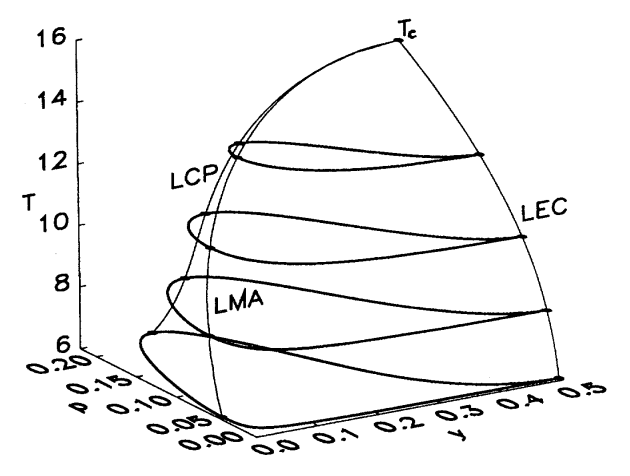
\includegraphics[width=0.5\textwidth]{binodal_mueller_serot.png}
	\caption{Exemplo de superfície binodal em um diagrama $T \times p \times y$ ($y$ indica a fração de prótons) para uma transição líquido-gás na matéria nuclear.}
	\label{Fig:binodal}
\end{figure}

\begin{figure}
	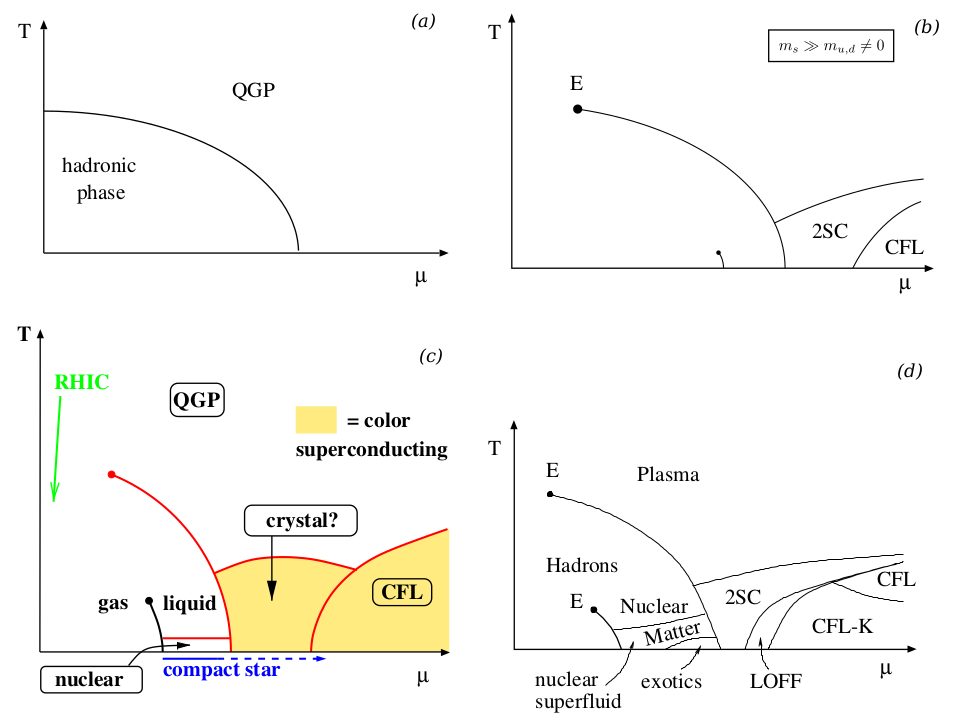
\includegraphics[width=\textwidth]{FigBuballa.png}
	\caption{Figura mostrando o diagrama $T\times \mu$ em sua forma conceitualmente mais simples \emph{(a)} e levando em conta resultados teóricos que preveem diversas outras fases da matéria de quarks e glúons, cada uma com propriedades particulares \emph{(b-d)}.}
\label{FigBuballa}
\end{figure}

%% Se for falar de Chiralidade, vai ser aqui ou em lugar próprio, antes de 'Condensados e outras fases'. Vide info que extraí do Stephanov 2004:
%\subsection{Chiralidade}
% * In QCD the two coexisting phases are hadron gas (lower T ), and quark-gluon
% plasma (higher T ). What distinguishes the two phases?
% * As in the case of water and
% vapor, the distinction is only quantitative, and more obviously so as we approach the
% critical point. Rigorously, there is no good order parameter which could distinguish
% the two phases qualitatively.
% * Deconfinement, although a useful concept to discuss the transition
% from hadron to quark-gluon plasma, strictly speaking, does not provide a good order
% parameter.
% * There is an idealization of QCD where the distinction between the hadron gas
% and quark gluon plasma is sharp. It describes the world with massless quarks
% * In this limit of QCD with 2 massless quarks (up and down) the chiral symmetry
% is exact
% * Although interactions respect this symmetry, it is sponta-
% neously broken in the QCD vacuum
% * At sufficiently high T, The chiral symmetry is restored. The two phases must be
% separated by a thermodynamic singularity – a phase transition. (T da transição é T_c)
% * In QCD, lattice calculations show that this singularity is a second order phase
% transition if T c is approached at μ B = 0
% * At other values of
% μ B the critical temperature T c is different, but the line of transitions T c (μ B ) cannot
% terminate, since any path from the vacuum T = μ B = 0 to the high T phase must
% cross a singularity. Somewhere in the midst of the phase diagram the order of the
% transition should change to first order
% * Once the quark mass m q is turned
% back on, the distinction between the
% symmetric and broken phases is blurred,
% and the second order phase transition
% is replaced by a smooth crossover

% Marcus: we concentrate on the high-$\mu$ and low-T with the aim of exploring the expected chiral phase transition which has significant impllications for the possible existencde of quark stars.

%Chiral symmetry breaking/restoring: evidências Quark Matter 2015 \url{https://www.bnl.gov/newsroom/news.php?a=25973#phase} \note{Falar do tratamento em simetria chiral.}

%Dentro do QGP se espera que haja uma restauração da simetria chiral. Pelo que entendi o problema é o seguinte: Se os quarks não tivessem massa, não haveria distinção dos quarks devido à chiralidade. Nos hádrons, eles se vestem de gluons e tem uma massa apreciável, mas dentro do QGP eles ficariam nus e com uma massa que ``tende'' a zero, restaurando a simetria chiral (não lembro onde li isso). Nesse caso dá pra mostrar que, ao se considerar simetria chiral, a região de crossover é uma transição de fase de segunda ordem, mas que ao ``religar'' a massa, a região de transição fica contínua (``blurred'' no Stephanov, arXiv: 0402115). Nesse caso o ponto é tricrítico (ver Stephanov).

%%%%%%%%%%%%%%%%%%%%%%%%%%
%\subsection{Ponto Crítico}

Ao se determinar a transição de fase a $\mu = 0$, fazendo a aproximação de que a massa dos quarks é nula, é possível mostrar que a transição de fases é de segunda ordem. Assim, em algum ponto do diagrama de fases, existe um \emph{ponto crítico} onde ocorre a mudança do tipo de transição de fase \cite{Stephanov2004}. Assim, se compararmos as fases que ocorrem em ambos os lados da linha de transição de fases, iniciando em $T = 0$, à medida que nos deslocamos em direção ao ponto crítico, percebemos que a distinção em primeira ordem entre as fases vai ficando progressivamente menor, até que após o ponto crítico a diferença entre elas deixa de existir. Esse tipo de fenômeno crítico é o mais comum em matéria condensada. Tratando o caso real de massas diferentes de zero, a região em que a transição de fases é de segunda ordem se torna uma transição do tipo \emph{crossover}~\cite{Stephanov2004}.

A determinação do ponto crítico é, a princípio, uma tarefa bem definida, bastando determinar a função de partição $\mathcal{Z}$ e a partir dela determinar o ponto onde a transição de fase deixa de ser de primeira ordem. Para $\mu = 0$, podemos determinar a equação de estado para a QCD como função de $T$ utilizando LQCD, porém para $\mu \neq 0$, ocorrem problemas de cálculo (\emph{sign problem}~\cite{Stephanov2004}).

%Ao se determinar a função de partição para $\mu = 0$, é possível restringir o cálculo a um conjunto relativamente pequeno de configurações escolhidas aleatoriamente, pois a probabilidade de cada estado é proporcional a $e^{-S}$ -- onde $S$ é uma função estritamente positiva dos valores dos campos nos pontos da rede~--. Dessa forma o número necessário de configurações escolhidas aleatoriamente para se atingir um resultado razoável é pequeno se comparado ao número total de configurações. Para $\mu \neq 0$, no entanto, $S$ é complexa, levando a dificuldades em determinar quais são as configurações mais prováveis e qual o número de configurações que devem ser levadas em conta. Para alguns casos específicos --~como, por exemplo, $\mu$ complexo, ou se $m_u = m_d$ e $\mu_u = -\mu_d$~--, $S$ assume valores positivos, eliminando essa dificuldade~\cite{Stephanov2006}.

Em todo caso, experimentalmente o ponto crítico pode ser investigado através de flutuações de observáveis entre diferentes eventos. Esse tipo de investigação é objeto de pesquisa em experimentos no RHIC/BNL, SPS/CERN, e será também investigado no GSI~\cite{Buballa,Stephanov2006}. A Figura~\ref{FigRHIC}\cite{RHIC} mostra a área do diagrama de fases abrangida pelo RHIC e a posição especulada do ponto crítico.

\begin{figure}[!htb]
	\centering
	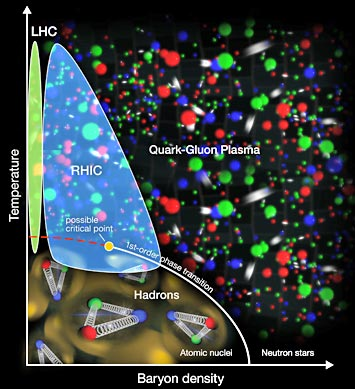
\includegraphics[width=7cm]{critical-point.jpg}
	\caption{Figura mostrando o diagrama de fases e as regiões que podem ser exploradas através dos experimentos realizados no RHIC (azul) e no LHC (verde).\label{FigRHIC}}
\end{figure}

%%%%%%%%%%%%%%%%%%%%%%%%%%%%%%%%%%%%%%%
%\subsection{Condensados e outras fases}

Além das fases hadrônica e de QGP, outras fases são esperadas para a matéria da QCD. Dependendo das condições termodinâmicas do sistema, pode ser vantajosa para a minimização da energia a formação de outras fases: para altas densidades e baixas temperaturas, a matéria nuclear deve exibir condensação de píons \cite{Glendenning,Schaefer}. Para densidades de algumas vezes a densidade de saturação da matéria nuclear, deve ocorrer a consação de kaons (quando consideramos também o quark $s$)
%\note{No arXiv:1010.5788v1 diz que devido àqueles pulsares com grande massa (ver PRC 89 055207 2014) essas possibilidades devem ser descartadas (provavelmente tem a ver com a grande massa e o fato de que a EOS fica mais ``soft'' com hyperons, o que não suportaria tal massa. Apesar de que eu acredito que um artigo da Débora dos que eu li que mostrava que dava pra ter uma equação com hyperons que suportava massas maiores.). Deve haver consequências do surgimento para a EOS, falar quais são e que são interessantes.}.

Para densidades altas e a baixas temperaturas, deve ocorrer a formação de uma fase ``supercondutora de cor'' (região sombreada da Figura~\ref{FigBuballa} \emph{(c)}). Isso se deve à formação de pares de quarks devida à intensa interação entre as partículas --~que é muito atrativa em alguns canais~\cite{Weber}~--, em uma situação análoga àquela que ocorre em supercondutores com a formação de pares de elétrons.

Como os quarks existem em sabores e cores diferentes, e possuem massas distintas, o diagrama de fases nessa região deve ser bastante complexo. Na Figura~\ref{FigBuballa}, subfiguras \emph{(b)} a \emph{(d)} temos representações esquemáticas do diagrama de fases incluindo as supercondutoras. As previsões diferentes se devem a suposições diferentes utilizadas ao se determinar as fases da matéria.


%% Outras informações
%``QCD phenomenology at finite temperature and baryon number density is one of te least explored regimes of the theory.'' (Stephanov, arXiv:hep-ph/0402115v1). 
%Apesar de tudo, poucas são as informações concretas que se tem sobre o diagrama de fases da QCD. Atualmente as fontes de informação se limitam à matéria nuclear e mesmo os cálculos teóricos utilizando a lagrangiana da QCD se limita ao eixo $\mu = 0$. Mas e as URHICs e os jatos, o jet-quenching?.\note{needs info}
%Cálculo da equação de estado e determinação do diagrama de fases, explorá-lo para procurar fases interessantes e outras coisas interessantes, como o QGP. Falar que algumas regiões podem ser exploradas através de colisões de íons pesados, outras de estrelas, muitas regiões estão dentro dos limites energéticos dos aceleradores de partículas existentes ou em construção. Falar sobre as linhas de coexistência de fases.
%Falar que outras características do sistema, como o campo magnético a que ele está submetido podem mudar a posição do ponto crítico, inclusive fazendo com que ele deixe de existir (isso quer dizer o que? que a transição de primeira ordem continua até que a linha toque o eixo da temperatura, ou simplesmente toda a linha deixa de existir se tornando um crossover?). Entra a estranheza aqui também, ou em outro lugar?
%Como se espera que haja desconfinamento no centro das estrelas, é importante estudar em quais regiões do diagrama de fases isso ocorre, pra identificar se isso pode ou não ocorrer em uma estrela. A ocorrência pode ser peça chave para explicar a massa de estrelas observadas recentemente (é isso?)

A solução das equações de movimento obtidas à partir da lagrangiana da QCD para o caso do QGP não é simples. Enquanto ao se tratar de quarks confinados podemos utilizar os métodos perturbativos desenvolvidos para a QED devido ao pequeno acoplamento entre quarks e glúons, quando no limite de matéria densa, o acoplamento entre essas partículas cresce e torna os resultados dos métodos perturbativos inadequados. Além disso, devido às dificuldades encontradas utilizando a LQCD para $\mu \neq 0$, uma alternativa para a investigação do diagrama de fases é a de utilizar modelos que tenham propriedades similares à QCD. 

A investigação do diagrama de fases é um exemplo de situação em que o emprego da LQCD não é viável, mas que pode ser explorado através de modelos. Outro resultado importante da aplicação de modelos é o cálculo da equação de estado, que pode então ser utilizada para a elaboração de modelos de propriedades estelares. Por outro lado, o poder preditivo dos modelos é certamente reduzido devido ao emprego de parâmetros e de aproximações, o que leva a uma constante necessidade de comparação com outras fontes de informação~\cite{Buballa}.

%Nesse sentido, três categorias de modelos foram desenvolvidas: modelos fenomenológicos, modelos dinâmicos e modelos autoconsistentes com base na equação de Dyson-Schwinger~\cite{Weber}. Exemplos de modelos amplamente utilizados para substituir a QCD são o \emph{MIT Bag Model} e o Modelo de Nambu--Jona-Lasinio, discutidos adiante.\note{Weber diz que o MIT é fenomenológico, o NJL é dinâmico? Que equação é essa de Dyson-Schwinger?}

%%%%%%%%%%%%%%%%%%%%%%%%%%%%%%%%%%%%%%%%%%%%%%%%%%%%%%%%%%%%%%%%%%%%%%%%%%%%%%%%%
\section{Modelos}

%%%%%%%%%%%%%%%%%%%%%%%%%%
%\subsection{MIT Bag Model}

%O modelo da ``sacola do MIT'' (MIT Bag Model) foi desenvolvido na tentativa de descrever a massa dos hádrons em termos das massas dos quarks que os constituem, sendo também utilizado para descrever a própria matéria de quarks. A premissa básica do modelo é a de assumir que os quarks ficam confinados em uma região (a ``sacola'') e que o movimento dentro de tal região é livre. O confinamento na região da sacola não é dinâmico, mas imposto pelas condições de contorno. Assim, para que exista estabilidade, uma constante $B$ correspondendo a uma contribuição positiva na energia e negativa na pressão é adicionada, sendo que ela é tratada como um parâmetro livre. O valor mais apropriado de tal constante é, para o caso da descrição das massas hadrônicas, $B^{1/4} = \np[MeV]{145}$, mas tal valor não é necessariamente adequado para a descrição da matéria de quarks.

%%%%%%%%%%%%%%%%%%%%%%%%%%%%%%%%%%%%%%%%%%
%\subsection{Modelo de Nambu--Jona-Lasinio}

O modelo de Nambu--Jona-Lasinio (NJL) é um modelo fenomenológico que originalmente tratava da interação de nucleons através de uma interação de dois corpos, em uma analogia à teoria BCS da supercondutividade~\cite{Buballa}. A lagrangiana desse modelo é dada por
\begin{equation}
	\mathcal{L} = \bar{\psi}(i\gamma^\mu\partial_\mu - m)\psi + G[(\bar{\psi}\psi)^2 + (\bar{\psi}i\gamma_5\vec{\tau}\psi)^2],
\end{equation}
%
onde $m$ é a massa do nucleon, $\vec{\tau}$ é uma matriz de Pauli atuando no espaço de isospin, $G$ é uma constante de acoplamento e $\psi$ é o campo associado ao nucleon \cite{Buballa}.

Hoje, no entanto, o modelo é reinterpretado em termos de quarks ($u$ e $d$ em SU(2), e $u$, $d$ e $s$ em SU(3)) com a mesma forma para a lagrangiana -- porém $\psi$ representa o campo associado aos quarks~--. O modelo tem deficiências tanto em suas versões de dois quanto de três quarks, devidas ao uso de uma interação efetiva de contato~\cite{Klevansky}, o que resulta em uma ausência do confinamento observado para os quarks (o que não era um problema já que o modelo foi desenvolvido antes mesmo que a QCD e o seu objetivo original era o de descrever a interação entre nucleons, cujo confinamento não existe). No entanto, em situações onde não há confinamento -- como no caso do QGP --, ou em situações onde tal propriedade não traz contribuições significativas, o modelo pode ser empregado. O ponto forte do modelo é que ele pode ser desenvolvido e forma a incorporar todas as simetrias globais da QCD, permitindo uma análise de mecanismos de quebra de simetria dinâmicos~\cite{Vogl}.

%\note{Se o NJL não descreve a saturação~\cite{japoneses}, dizer nesse §. Confinamento: não entendo essa treta direito, mas agora estou achando que é o seguinte: os quarks hadronizam, isto é, confinam. Até aí, blz, mas o modelo não consegue lidar com isso. Não tem como ele prever que os campos de três quarks vão se ligar de tal formal que se estabeleça um estado ligado. Ou tratamos os campos como sendo de quarks e descrevemos o QGP, ou tratamos os campos como sendo de nucleons. Aí ficamos com uma descrição que é uma merda, pois não consegue nem descrever a saturação da matéria nuclear. Mas, vendo pelo lado bom, é uma merda que tem simetria chiral. Então o negócio é adicionar termos até que o esquema consiga descrever a saturação da matéria nuclear. Pelo que entendo, o termo adicionado é o escalar-vetor. O vetor é adicionado por outras razões.}

O modelo NJL originalmente inclui somente interações escalar e pseudo escalar. A inclusão de um termo escalar-vetorial no modelo NJL é capaz de mudar a dependência da energia de ligação na densidade, e a dependência desta na massa, o que faz com que o modelo NJL consiga descrever a saturação da matéria nuclear adequadamente~\cite{Koch}. Assim, o modelo pode ser empregado na descrição da fase de hádrons, porém com a vantagem de apresentar simetria quiral, diferentemente de modelos que assumem uma massa não nula para os nucleons. 

Outro termo relevante na descrição da matéria formada por quarks é o vetor-isoescalar. A importância de tal interação para a descrição da matéria nuclear a densidades intermediárias é bem conhecida (sendo essencial no modelo de Walecka~\cite{Advances16}, por exemplo) e recentemente vem sendo utilizada como uma extensão do modelo NJL~\cite{Abuki, NJLv}.
%\note{Enumerar brevemente (uma linha ou duas) as razões para a inclusão dessa interação.}.

%composta somente por férmions devido à sua importância na determinação de propriedades a densidades intermediárias da matéria nuclear, e a correta reprodução de medidas de diferenças de fluxo elíptico entre nucleons e anti-nucleons, bem como entre kaons e anti-kaons em experimentos executados no RHIC. 

O efeito de ambas as interações discutidas acima no diagrama de fases da QCD é a de enfraquecer a transição de primeira ordem, sendo que um aumento da interação força o ponto crítico a se deslocar para valores menores de temperatura, bem como para valores mais altos de potencial químico~\cite{NJLv, japoneses}.

Com a inclusão das interações vetorial e escalar-vetorial, o modelo de Nambu--Jona-Lasinio passa a ser descrito em SU(3) pela lagrangiana
\begin{equation}
	\mathcal{L}_{\rm{NLJ}} = \bar{\psi}_i[i\gamma_\mu\partial^\mu - \hat{m}_f]\psi_i + \mathcal{L}_{\textrm{sym}} + \mathcal{L}_{\textrm{det}} + \mathcal{L}_{\textrm{v}} + \mathcal{L}_{\textrm{sv}},
\end{equation}
%
onde
\begin{align}
	\mathcal{L}_{\textrm{sym}} &= G_S\sum_{a=0}^8[(\bar{\psi}_i\lambda_a\psi_i)^2 + (\bar{\psi}_i i\gamma_5\lambda_a\psi_i)^2 \\
	\mathcal{L}_{\textrm{det}} &= -K\{\det[(\bar{\psi}_i(1+\gamma_5)\psi_i] + \det[\bar{\psi}_i(1-\gamma_5)\psi_i]\} \\
	\mathcal{L}_{\textrm{v}} &= -G_V \sum_{a=0}^8[(\bar{\psi}_i\gamma^\mu\lambda_a\psi_i)^2 + (\bar{\psi}_i\gamma^\mu\gamma_5\lambda_a\psi_i)^2] \\
	\mathcal{L}_{\textrm{sv}} &= - G_{sv}^i \left[(\bar{\psi}_i\psi_i)^2 + (\bar{\psi}_i i \gamma_5 \vec{\tau}\psi_i)^2\right](\bar{\psi}_i\gamma^\mu\psi_i)^2.
\end{align}
%
Nas expressões acima, o índice $i$ denota os casos de matéria nuclear ($i = N$) ou matéria de quarks ($i = q$), $\psi_i$ representa os campos fermiônicos de quarks ou nucleons, $\vec{\tau}$ representa as matrizes de Pauli no espaço de isospin, $q$ representa a carga elétrica, e $\hat{m}_f$ é a matriz de massa. Os termos $\mathcal{L}_{\textrm{sym}}$, $\mathcal{L}_{\textrm{det}}$, $\mathcal{L}_{\textrm{v}}$, e $\mathcal{L}_{\textrm{sv}}$ correspondem a uma interação de quatro pontos no espaço de sabor, à interação de t'Hooft (para três sabores equivale a uma interação de seis pontos), à interação vetorial, e à vetor-escalar. 

A lagrangiana $\mathcal{L}_{\textrm{NLJ}}$ acima descreve então tanto a fase de hádrons, quanto a de quarks, porém as constantes assumem valores diferentes, sendo que para hádrons $G_{sv}^N = 0$. Como o modelo NJL é não renormalizável, é necessário realizar a regularização, sendo que ela será feita via \emph{cutoff}, fornecendo um parâmetro $\Lambda$ adicional. Tais constantes são então ajustadas para reproduzir as massas dos mésons $\pi$, $K$ e $\eta'$, além da constante de decaimento do méson $\pi$.

%Apesar de o modelo de Nambu--Jona-Lasinio ter sido desenvolvido para tratar a interação entre nucleons, ele não é capaz de descrever adequadamente a saturação da matéria nuclear simétrica. No entanto, ao se introduzir uma interação do tipo escalar-vetor e isoescalar vetor de oito pontos\note{scalar-vector and isoscalar-vector eight-point interaction}, tal propriedade é bem reproduzida \cite{japoneses}. Dessa forma, tanto a fase de hádrons, quanto a fase de quarks podem ser descritas através da lagrangiana
%\begin{equation}
%\begin{split}
%	\mathcal{L}_i &= \bar{\psi}_i i \gamma^\mu\partial_\mu\psi_i + G_s^i\left[(\bar{\psi}_i\psi_i)^2 + (\bar{\psi}_ii\gamma_5\vec{\tau}\psi_i)^2\right] \\
%	&\phantom{=} - G_v^i(\bar{\psi}_i\gamma^\mu\psi_i)(\bar{\psi}_i\gamma_\mu\psi_i) \\
%	&\phantom{=} - G_{sv}^i\left[(\bar{\psi}_i\psi_i)^2 + (\bar{\psi}_i \gamma_5\vec{\tau}\psi_i)^2\right](\bar{\psi}_i\gamma^\mu\psi_i)(\bar{\psi}_i\gamma_\mu\psi_i),
%\end{split}
%\end{equation}
%
%onde o índice $i$ denota os casos de matéria nuclear ($i = N$) ou matéria de quarks ($i = q$), $\psi_i$ representa os campos fermiônicos de quarks ou nucleons e $\vec{\tau}$ representa as matrizes de Pauli no espaço de isospin. As constantes $G_s^i$, $G_v^i$ e $G_{sv}^i$ representam os acoplamentos dos termos ??\note{o primeiro é o que?}, vetor-vetor, e escalar-vetor e isoescalar-vetor. Os dois primeiros termos na lagrangiana acima são os que aparecem na lagrangiana original do termo de Nambu--Jona-Lasinio.\note{Ver mais observações e condensá-las aqui ou no § anterior.}

%%%%%%%%%%%%%%%%%%%%%%%%%%%%%%%%%%%%%%%%%%%%%%%%%%%%%%%%%%%%%%%%%
%\subsection{Modelo de Nambu--Jona-Lasinio com interação vetorial}

%Um modelo amplamente utilizado para a descrição da matéria nuclear é o Modelo de Walecka. Nesse modelo, os nucleons interagem através da troca de mésons. Em sua versão mais simples, são considerados os mésons $\sigma$ e $\omega$, correspondendo a uma interação escalar-isoescalar e a uma interação vetor-isoescalar. O sucesso de tal modelo em descrever várias propriedades de núcleos e da matéria nuclear é um atestado da importância de ambos os tipos de interação, mesmo que para a descrição adequada de algumas propriedades, seja necessária uma versão mais elaborada do modelo. 


%NJL: In its original form, this model was constructed as a pre-QCD theory of nucleons that interact via an effective two-body interaction. This today is reinterpreted as a theory with quark degrees of freedom. Of primary importance is the fact that the lagrande density of this model is constructed such that the symmetries of QCD that are also observed in nature are part and parcel of it. One of the most important of these is chiral symmetry, which is essential to the understanding of the lightest hadrons. [...] The NJL model int the two-flavors or the appropriate generalization to three-flavors, has shortcomings that are a consequence of the use of and effective contact interaction. Tis interactions is not confining; so it should only be applied to properties for which confining is not expected to be essential. {Como é o caso do QGP} (Klevansky, Rev. Mod. Phys. 64 649 (1992)

%``The Nambu and Jona-lasinio model dates back to the early sixties with the apearance of two pioneering papers [...]. It combines elements of Heisenber's nonlinear spinor theory with the observations of a close analogy between the properties of Dirac particles and the quasi-particle excitations which appear in the BCS theory of superconductivity.

%By that time QCD, the gauge theory of Strong Interactions of quarks and gluons, did not yet exist. When QCD arrived the NJL model was soon critizised and more or less abandoned, mainly because of its non-fundamental nature, and because its non-renormalizability was considered prohibitive by many theorists. It regained popularity when it was realized that the model shares some conceptually important features with low energy QCD. {Mas QGP é high energy pra cacete, não? comofaz?}

%The NJL model is an effective lagrangian of relativistic fermions interacting through local fermion-fermion couplings. [...] The strength of this model is that it can be designed to incorporate all global symmetries of QCD and enables one to `see' dynamical symmetry breaking mechanisms at work.''(Vogl and Weise)



%%%%%%%%%%%%%%%%%%%%%%%%%%%%%%%%%%%%%%%%%%%
\section{Proposta de trabalho e cronograma}

Dada da relevância do conhecimento das propriedades das fases e dos limites entre elas no diagrama de fases da QCD, tanto no que tange ao entendimento das propriedades da matéria constituída por quarks, quanto em suas implicações em colisões, estrelas e no entendimento dos momentos iniciais após o Big Bang, propomos a investigação da transição hádron-QGP em um modelo de duas fases. Para a descrição das fases, utilizamos as duas versões do modelo de Nambu--Jona-Lasinio descritas acima, sendo que a versão que inclui a interação vetorial será utilizada para descrever a fase de hádrons e a versão sem a interação vetorial descreverá a fase de QGP.

Na Referência~\cite{Rafael} o diagrama de fases da QCD e a transição de fase hádrons-QGP para matéria assimétrica são analisados em busca de propriedades que podem ser relevantes para a descrição de colisões de íons pesados. A análise também se dá por meio de um modelo de duas fases, porém a descrição é feita através do modelo MIT Bag Model~\cite{Buballa} --~incluindo glúons~-- para a fase de QGP, enquanto a fase de hádrons é descrita pelo Modelo de Walecka Não-Linear~\cite{Advances16}. A não-linearidade se refere a auto-interação do campo escalar, sendo que o modelo também inclui uma interação vetorial-isovetorial. Nesse modelo é fundamental a presença do canal vetorial. Os cálculos realizados pelos autores trata a possibilidade de matéria assimétrica, já que esse tipo de sistema apresenta propriedades diferentes daquelas de sistemas simétricos (Ref. [25-29,30] em~\cite{Rafael}).

Embora os autores não incluam outras fases na análise (supercondutoras, por exemplo), os efeitos da inclusão de píons, kaons e híperons na fase de hádrons é investigado. Assim, a coexistência de fases (superfície binodal) é determinada em três situações: \emph{(a)} matéria hadrônica constituída por nucleons, \emph{(b)} matéria hadrônica constituída por nucleons e píons, e \emph{(c)} matéria hadrônica constituída por nucleons, híperons, píons e kaons (com estranheza líquida nula), sempre coexistindo com matéria de quarks constituída por quarks $u$ e $d$. Além disso, a população de cada partícula como função da densidade é calculada de maneira a verificar em que condições ocorrem as condensações de píons e kaons.

Com o objetivo de comparar os resultados com os da Referência~\cite{Rafael}, também incluiremos píons e kaons na fase hadrônica, bem como consideraremos a possibilidade de matéria assimétrica a temperatura finita. Também calcularemos a superfície binodal e as populações de partícula. Através disso, seremos capazes de determinar em que condições ocorre a transição de fase hádron-QGP para os modelos empregados, bem como analisaremos a possibilidade de formação de condensados. A obtenção de tais resultados será feita através da determinação das equações de estado para a matéria na fase desejada (energia, pressão, número de partículas), que por sua vez é obtida através do potencial termodinâmico que pode ser calculado a partir da lagrangiana do sistema. Para determinar a coexistência de fases utilizaremos as condições de Gibbs.

\vspace{1cm}

%%%%%%%%%%%%%%%%%%%%%%%
\subsection{Cronograma}

Devido ao fato de que o afastamento para docentes de instituições de ensino superior federais é de no máximo 12 meses, o cronograma abaixo contempla somente tal período. O início das atividades se dará em 01/02/2016, sendo finalizadas em 31/01/2017. As etapas a serem executadas são:
\begin{itemize}
\item Reproduzir os cálculos analíticos existentes.
\item Preparar cálculos numéricos para o modelo em SU(2),
  correspondendo a uma fase hadrônica contendo nucleons e uma fase de
  quarks contendo apenas quarks $u$ e $d$.
\item Introduzir condensados bosônicos e comparar com resultados para
  binodal apresentados em \cite{Rafael}.
\item Realizar cálculos analíticos e numéricos para as versões SU(3)
  dos modelos, contendo nucleons e híperons na fase hadrônica e os 3
  quarks mais leves, $u,d$ e $s$ na fase de quarks.
\item Preparar códigos numéricos para determinar as binodais e o
  diagrama de fases da QCD. 
\end{itemize}

%%%%%%%%%%%%%%%%%%%%%%%%%%%%%%%%%%%%%%%%%%%%%%%%%%%%%%%%%%%%%%%%%%
\section{Inserção no Grupo de Física Nuclear e de Hádrons da UFSC}

O grupo de Física Nuclear e de Hádrons da UFSC, no momento, é um dos grupos
com maior número de pesquisadores dedicando-se a esse tema no Brasil,
constituindo-se de 5 professores do Campus de Florianópolis, um do Campus de
Curitibanos, 1 do Campus de Blumenau, 1 pós-doc, 12 doutorandos, 5 mestrandos e vários alunos de
iniciação científica. O grupo conta com uma ótima infra-estrutura logística e
computacional, incluindo acesso a um cluster de alto desempenho. As áreas
de interesse mais recente têm sido transições de fase líquido-gás,
e hádrons-quarks desconfinados, {\it pasta phase} e matéria de hádrons e de
quarks sujeitas a campos magnéticos fortes. Tais linhas de pesquisa têm sido
aplicadas a astrofísica nuclear e a interpretação de resultados oriundos de
colisões de íons pesados.

O presente projeto adequa-se perfeitamente aos interesses do grupo.


\chapter{Fase de Hadrons: eNJL}

\section{Simetria quiral}

Ver discussão em Ref.\cite{Vogl}
% Vogl, U., and W. Weise. - Progress in Particle and Nuclear Physics 27 (1991): 195-272 - The Nambu and Jona-Lasinio model: its implications for hadrons and nuclei
\section{Termodinâmica}

Temos que $dS$ ou $dU$ -- deve ser $dU$, pois o potencial químico é a ``quantidade de energia ganha ao se inserir mais uma partícula no sistema'' -- tem um termo $\mu dN$. Vamos trabalhar com densidade bariônica, mas essa densidade é só o número de partículas $N$ dividido pelo volume (as outras variáveis também serão trabalhadas divididas pelo volume). Logo, temos $\mu d\rho$. Por isso, temos que $\mu = d\epsilon/d\rho$, onde $\epsilon$ é a densidade de energia $\epsilon = E/V$. 

Glendenning\cite{Glendenning}:
Degenerate ideal Fermi gas: ideal pois não tem interações entre as partículas, degenerado pois todos os estados até uma certa energia -- a energia de Fermi -- estão ocupados. Nesse caso, a soma sobre todos os estados ocupados (que são autoestados de momento, pois não há interação) deve se dar sobre o momento. Isso pode ser escrito como a integral
\begin{equation}
	\int_0^{k_f} \frac{d^3k}{(2\pi^3)}.
\end{equation}
%
(pelo que lembro, é um cálculo realizado em um octante, contando quantos estados existem entre $p$ e $p+dp$ levando-se em conta que são ondas estacionárias em uma caixa de lado $L$. Nesse caso $k$ (que está associado ao momento) é um inteiro vezes o comprimento de onda dividido por dois. Tentar achar isso Ref [63] do Glendenning.

O gás pode ser considerado degenerado se $T \ll E_F = \sqrt{k_F^2 + m^2}$.

A densidade é obtida simplesmente somando os estados ocupados. A energia é calculada somando a energia de cada estado ocupado. A pressão eu não sei:
\begin{align}
	\rho &= \\
	\epsilon &= \\
	p &=
\end{align}

In thermodynamics, chemical potential, also known as partial molar free energy, is a form of potential energy that can be absorbed or released during a chemical reaction. It may also change during a phase transition. The chemical potential of a species in a mixture can be defined as the slope of the free energy of the system with respect to a change in the number of moles of just that species. Thus, it is the partial derivative of the free energy with respect to the amount of the species, all other species' concentrations in the mixture remaining constant, and at constant temperature. When pressure is constant, chemical potential is the partial molar Gibbs free energy. At chemical equilibrium or in phase equilibrium the total sum of chemical potentials is zero, as the free energy is at a minimum. \url{https://en.wikipedia.org/wiki/Chemical_potential}



%%%%%%%%%%%%%%%%%%%%%%%%%%%%%%%%%%%%%%%%%%%%
\section{Artigo: Pais, Menezes, Providência}
%%%%%%%%%%%%%%%%%%%%%%%%%%%%%%%%%%%%%%%%%%%%

Sobre o modelo\cite{Pais}:
\begin{quote}
The NJL model can be extended [...] to yield reasonable saturation properties of nuclear matter, the field $\psi$ being the nucleon field. An effective density dependent coupling constant is obtained if the following extended NJL (eNJL) Lagrangian density, which actually pushes chiral symmetry restoration to higher densities, is considered,
\begin{equation}\label{Eq:Lagrangiana_eNLJ_Pais}
\begin{split}
	\mathcal{L} &= \bar{\psi}(i\gamma^\mu\partial_\mu)\psi + G_s[(\bar{\psi}\psi)^2 + (\bar{\psi}i\gamma_5\vec{\tau}\psi)^2] - G_v(\bar{\psi}\gamma^\mu\psi)^2 \\
	&\phantom{=}- G_{sv}[(\bar{\psi}\psi)^2 + (\bar{\psi}i\gamma_5\vec{\tau}\psi)^2](\bar{\psi}\gamma^\mu\psi)^2 - G_\rho[(\bar{\psi}\gamma^\mu\vec{\tau}\psi)^2 + (\bar{\psi}\gamma_5\gamma^\mu\vec{\tau}\psi)^2] \\
	&\phantom{=}- G_{v\rho}(\bar{\psi}\gamma^\mu\psi)^2[(\bar{\psi}\gamma^\mu\vec{\tau}\psi)^2 + (\bar{\psi}\gamma_5\gamma^\mu\vec{\tau}\psi)^2].
\end{split}
\end{equation}
\end{quote}

Outras informações relevantes (ainda do artigo)\footnote{Qual é a função do termo em $G_{s\rho}$? Qual é o papel do termo em $G_v$? (Ver o que tem no Walecka).}:
\begin{itemize}
	\item Para a matéria nuclear, a degenerescência é $2 N_f$;
	\item O \emph{cutoff} $\Lambda$ é tal que a massa do nucleon no vácuo seja de 939 MeV, determinada variacionalmente;
	\item O termo proporcional $G_s$ simula uma repulsão de curto alcance entre os nucleons (chiral invariant);
	\item ``The term in $G_{sv}$ accounts for the density dependence of the scalar coupling. For the nuclear matter, the NJL model leads to binding, but the binding energy per particle does no have a minimum except at a rather high density where the nucleon mass is small or vanishing. The introduction of the $G_{sv}$ coupling term is required to correct this.''
	\item O termo proporcional a $G_\rho$ (isovetor-vetor) é incluido para descrever a matéria nuclear assimétrica (em isospin); 
\end{itemize}

A partir da lagrangiana \eqref{Eq:Lagrangiana_eNLJ_Pais}, é possível determinar\footnote{Como? Através de $\omega(T,\mu) = -\frac{T}{V} \ln \mathcal{Z}$?} o potencial termodinâmico\footnote{Potencial Grand-canônico, ou potencial de Landau.} por unidade de volume, dado por
\begin{equation}\label{Eq:potencial_termodinamico}
	\omega(\mu) = \varepsilon_{\rm{kin}} - G_s\rho_s^2 + G_v\rho^2 + G_{sv}\rho_s^2\rho^2 + G_\rho\rho_3^2 + G_{v\rho}\rho^2\rho_3^2 - \mu_p\rho_p - \mu_n\rho_n,
\end{equation}
%
onde
\begin{itemize}
	\item $\rho$ é a densidade bariônica, dada pela soma das densidades de nêutron e próton\footnote{São densidades numéricas de partículas, ou seja, representam o número de partículas por unidade de volume.}:
	\begin{equation}
		\rho = \rho_p + \rho_n.
	\end{equation}

	\item As densidades bariônicas de próton e nêutron são dadas por\footnote{De onde vem essa expressão para $\rho_i$. Explicar, explicar o momento de Fermi também.}
	\begin{equation}
		\rho_i = \int_0^{k_F^i}\frac{dp}{\pi^2}p^2; \qquad i = p,n; \quad k_F^i = \textrm{momento de Fermi},
	\end{equation}
	%
	ou, caso $\rho_i$ sejam conhecidos
	\begin{equation}\label{Eq:Mom_Fermi_a_partir_de_rho}
		p_F^i = \sqrt[3]{3\pi^2\rho_i}.
	\end{equation}
	
	\item $\mu_p$ e $\mu_n$ representam os potenciais químicos de próton e nêutron, respectivamente.
\end{itemize}

O termo cinético na expressão acima pode ser calculado através de (primeiro termo da Eq. (1) em \cite{PRC_68_035804_2003}, o resto é energia potencial)\footnote{Degenerescência: O 2 se refere às duas possibilidades de spin; Podemos ter um $N_f$ que representa o número de sabores. Acredito que o sinal não seja do termo cinético, então tem que retirar daqui. No programa em Fortran está definido sem esse sinal. Apesar de que o valor de $\varepsilon_{\rm{kin}}$ fica negativo sem esse sinal; energia cinética é estritamente positiva!.}
\begin{align}
	\varepsilon_{\rm{kin}} &= \langle\bar{\psi}(\vec{\gamma}\cdot\vec{p}\psi\rangle \\
	&= - 2 N_c\sum_i \int \frac{d^3p}{(2\pi)^3}\frac{p^2 + m_i M_i}{E_i}(n_{i-}-n_{i+})\theta(\Lambda^2 - p^2),
\end{align}
%
onde
\begin{itemize}
	\item A soma se dá sobre as espécies de partículas;
	\item $N_c$ representa o número de cores\footnote{No nosso caso, 1?};
	\item $\theta$ é a função degrau, $\Lambda$ é o \emph{cutoff};
	\item $n_{i\pm}$ são as funções de distribuição de Fermi para estados de energia positiva e negativa (respectivamente), dados por
	\begin{equation}
		n_{i\pm} = \frac{1}{1 + \exp(\pm[\beta(E_i\mp\mu_i)])}
	\end{equation}
	%
	onde $i = p, n$ (no nosso caso, no artigo é $u, d, s$) e $\beta = T^{-1}$
	\item $M_i$ é a massa constituinte do nucleon em questão (quark, no artigo).
	\item $E_i = \sqrt{p^2 + M_i^2}$
	\item $m_i$ no artigo são as massas (nuas?) dos quarks, e no nosso caso?\footnote{Ver isso.}
\end{itemize}

Se tomarmos $T \to 0$, temos que $n_{i-} \to 1$ e $n_{i+} \to 0$; Além disso, se o integrando só depende do módulo de $\vec{p}$, então (\cite{Glendenning}, p. 92)
\begin{equation}
	\int\frac{d^3p}{(2\pi)^3} \to \frac{1}{2\pi^2}\int p^2dp.
\end{equation}
%
Logo, temos
\begin{align}
	\varepsilon &= -2 N_c \frac{1}{2\pi^2}\sum_i \int p^2 dp \frac{p^2 + m_i M_i}{\sqrt{p^2 + M_i^2}} \theta(\Lambda^2 - p^2) \\
	&= -\frac{N_c}{\pi^2}\sum_i\left[\int \frac{p^4dp}{\sqrt{p^2 + M_i^2}}\theta(\Lambda^2 - p^2) + \int m_i M_i \frac{p^2 dp}{\sqrt{p^2 + M_i^2}}\theta(\Lambda^2 - p^2)\right]
\end{align}
%
Podemos utilizar as relações (\cite{Glendenning} p. 94\footnote{Na Ref. o primeiro termo da segunda expressão aparece sem o $k$ multiplicando, o que dimensionalmente está incorreto.})
\begin{align}
	\int \frac{k^4}{\sqrt{k^2 + m^2}} dk &= \frac{1}{4}\left[k^3\epsilon - \frac{3}{2} m^2k\epsilon + \frac{3}{2}m^4\ln\frac{\epsilon + k}{m} \right]\\
	\int \frac{k^2}{\sqrt{k^2 + m^2}} dk &= \frac{1}{2}\left[k\epsilon - \frac{1}{2}m^2\ln\frac{\epsilon + k}{m}\right] \label{Eq:Integ_momento_quad}
\end{align}
%
onde $\epsilon = \sqrt{k^2+m^2}$. Tomando o caso $m_i \to 0$\footnote{No prog. \texttt{eos\_enjl1-dens-assym- clean-rho-vr.f}: $\varepsilon \propto [F_2(M, k_F^i) - F_2(M, \Lambda)]$ ao invés de $\varepsilon \propto [F_2(M_i, \Lambda) - F_2(M_i, 0)]$; Isso se deve à retirada da contribuição do vácuo. Além disso, aparentemente os $M_i$ podem ser diferentes. No prog. são iguais, imagino que seja por considerarmos $m_n = m_p = m_N$.}, obtemos
\begin{equation}\label{Eq:Energia_kin}
	\varepsilon_{\rm{kin}} = -\frac{N_c}{\pi^2}\sum_i \Big[\underbrace{\frac{1}{8}\Big((2p^3 - 3M_i^2p)\sqrt{p^2 + M_i^2} + 3M_i^4\ln\frac{p + \sqrt{p^2 + M_i^2}}{M_i}\Big)}_{F_2(m,p)}\Big]_0^\Lambda
\end{equation}

A densidade escalar $\rho_s$ é dada por\footnote{De onde vem essa expressão?}
\begin{equation}\label{Eq:Dens_Escalar}
	\rho_s^i = \frac{M}{\pi^2}[F_0(M, p_F^i) - F_0(M, \Lambda)], \quad i = p, n,
\end{equation}
%
onde
\begin{equation}
	F_0(M, x) = \int_0^x \frac{dp}{\pi^2}\frac{p^2}{\sqrt{M^2 + p^2}}, \quad i = p, n.
\end{equation}
%
Utilizando a Equação~\eqref{Eq:Integ_momento_quad}, podemos reescrever a equação acima como\footnote{Esse $\pi^2$ no denominador está com cara de que não deveria estar aí. A parece um $\pi^2$ no denominador na definição de $\rho_s$ em termos de $F_0(M, x)$ e se eu deixar nos dois lugares, não há raízes para a equação do Gap. Por outro lado, mesmo que eu deixe, $\rho_s$ é menor que zero!}
\begin{equation}
	F_0(M, x) = \frac{1}{2\pi^2}\left[x\sqrt{x^2+M^2} - M^2 \ln \frac{x + \sqrt{x^2+M^2}}{M}\right].
\end{equation}

A massa\footnote{constituinte?} $M$ na equação acima é dada por\footnote{Essa equação é conhecida como \emph{Gap equation} (?).}
\begin{equation}\label{Eq:Gap}
	M = -2G_s\rho_s + 2G_{sv}\rho_s\rho^2,
\end{equation}
%
com $\rho_s = \rho_s^p + \rho_s^n$. Temos, portanto, uma interdependência entre as equações. Para que seja possível solucionar tais equações, podemos definir uma função $f(M)$ de tal forma que
\begin{equation}\label{Eq:Gap_zero}
	f(M) = M + 2G_s\rho_s - 2G_{sv}\rho_s\rho^2.
\end{equation}
%
Para solucionarmos a equação acima, basta utilizarmos uma rotina para encontrar zeros de funções, por exemplo biseção ou Newton-Raphson, encontrando o valor de $M$ para o qual $f(M) = 0$. A densidade escalar $\rho_s$ pode ser calculada através da expressão~\eqref{Eq:Dens_Escalar}\footnote{Na prática é mais fácil salvar o último valor de $\rho_s$ calculado pela rotina que tenta encontrar o zero da função $f(M)$.}.

Os potenciais químicos são dados por\footnote{Como essas expressões são calculadas?}
\begin{equation}\label{Eq:Potenciais_Quimicos}
	\mu_i = E_{p_F}^i + 2G_v\rho + 2G_{sv}\rho\rho_s^2 \pm 2G_\rho\rho_3+2G_{v\rho}\rho_3^2\rho \pm 2G_{v\rho}\rho^2\rho_3,
\end{equation}
%
onde $i = p,n$, os sinais superiores se referem ao caso de prótons, e $E_{p_F}^i = \sqrt{M^2 + (p_F^i)^2}$.

As equações de estado para pressão $P$ e densidade de energia $\varepsilon$ são dadas por\footnote{Como são calculadas?}
\begin{align}
	P &= -\omega(\mu) + \epsilon_0 \label{Eq:Pressao}\\
	\varepsilon &= -P + \mu_p\rho_p + \mu_n\rho_n. \label{Eq:Densidade_energia}
\end{align}

%%%%%%%%%%%%%%%%%%%%%%%%%%%%%
\section{Análise dimensional}
%%%%%%%%%%%%%%%%%%%%%%%%%%%%%

Devido ao fato de que $\hbar = c = 1$, adimensionais, e que não carregamos quaisquer unidades, é comum que algumas equações tenham dimensões discrepantes entre os membros esquerdo e direito, ou mesmo entre termos de um mesmo membro. Podemos acertar as dimensões multiplicando por potências de $\hbar c$. Nas unidades usuais em Física Nuclear, temos que $\hbar c = 197.326\rm{MeV}\cdot\rm{fm}$. Logo, todas as grandezas têm dimensões que envolvem MeV ou fm, ou uma combinação de ambos\sidenote{Note que de qualquer forma as unidades são atípicas, pois --~por exemplo~-- a unidade de massa é o eV, que na realidade tem dimensão de energia. Isso pode ser explicado através de $E^2 = p^2 c^2 + m^2 c^4$, onde assumimos que $c = 1$, adimensional.}:

\begin{itemize}
	\item Como $E^2 = p^2c^2 + m^2c^4$, temos $[E] = [m] = [p]$;
	\item Como $\rho = \bar{\psi}\gamma^0\psi$ é o número de partículas por unidade de volume, temos que $[\rho] = \rm{fm}^{-3}$
	\item O item acima implica que $[\psi] = \rm{fm}^{-3/2}$. Consequentemente, $[\rho_s] = [\bar{\psi}\psi] = \rm{fm}^{-3}$. 
	\item Como o potencial químico esta relacionado à variação de energia ao se adicionar ou retirar partículas do sistema, sua unidade é a de energia (MeV).
	\item O potencial termodinâmico $\omega$ é o potencial grande-canônico $\Omega$\footnote{Potencial de Landau} por unidade de volume, portanto tem dimensão de energia por unidade de volume ($\rm{MeV}\cdot\rm{fm}^{-3}$), assim como a densidade de energia $\varepsilon$ e a pressão $P$.
\end{itemize}

Dessa forma, as equações discutidas acima precisam ter suas unidades checadas e --~quando necessário~-- corrigidas, de forma a ficarem consistentes. Temos então:
\begin{fullwidth}
\begin{itemize}

\item O potencial termodinâmico (por unidade de volume) $\omega$ deve ter dimensão energia por volume (no nosso caso, $\rm{MeV}/\rm{fm}^3$):
\begin{equation}
	\underbrace{\omega}_{\frac{\rm{MeV}}{\rm{fm}^3}} = \underbrace{\varepsilon_{\rm{kin}}}_{\frac{\rm{MeV}}{\rm{fm}^3}} - \underbrace{G_s}_{\rm{fm}^2}\underbrace{\rho_s^2}_{\rm{fm}^{-6}} + \underbrace{G_v}_{\rm{fm}^2}\underbrace{\rho^2}_{\rm{fm}^{-6}} + \underbrace{G_{sv}}_{\rm{fm}^8}\underbrace{\rho_s^2\rho^2}_{\rm{fm}^{-12}} + \underbrace{G_\rho}_{\rm{fm}^2}\underbrace{\rho_3^2}_{\rm{fm}^{-6}} + \underbrace{G_{v\rho}}_{\rm{fm}^2}\underbrace{\rho^2\rho_3^2}_{\rm{fm}^{-12}} + \underbrace{\mu_p}_{\rm{MeV}}\underbrace{\rho_p}_{\rm{fm}^{-3}} + \underbrace{\mu_n}_{\rm{MeV}}\underbrace{\rho_n}_{\rm{fm}^{-3}}.
\end{equation}
%
Os termos envolvendo as constantes $G_i$ necessitam ser multiplicados por $\hbar c$, cuja dimensão é $\rm{MeV}\cdot\rm{fm}$, resultando na dimensão $\rm{MeV}/\rm{fm}^3$ para tais termos.

\item A pressão deve ter unidade de energia por unidade de volume ($\rm{MeV}/\rm{fm}^3$):
\begin{equation}
	\underbrace{P}_{\frac{\rm{MeV}}{\rm{fm}^3}} = - \underbrace{\omega}_{\frac{\rm{MeV}}{\rm{fm}^3}} + \underbrace{\varepsilon_0}_{\frac{\rm{MeV}}{\rm{fm}^3}},
\end{equation}
%
assim como a densidade de energia
\begin{equation}
	\underbrace{\varepsilon}_{\frac{\rm{MeV}}{\rm{fm}^3}} = - \underbrace{P}_{\frac{\rm{MeV}}{\rm{fm}^3}} + \underbrace{\mu_p}_{\rm{MeV}}\underbrace{\rho_p}_{\rm{fm}^{-3}} + \underbrace{\mu_n}_{\rm{MeV}}\underbrace{\rho_n}_{\rm{fm}^{-3}},
\end{equation}
%
e podemos ver que ambas estão com todas as dimensões corretas.

\item A equação para o cálculo da massa
\begin{equation}
	\underbrace{M}_{\rm{MeV}} = -2 \underbrace{G_s}_{\rm{fm}^2} \underbrace{\rho_s}_{\rm{fm}^{-3}} + 2 \underbrace{G_{sv}}_{\rm{fm}^8}\underbrace{\rho_s\rho^2}_{\rm{fm}^{-9}}
\end{equation}
%
necessita ser multiplicada por $\hbar c$ no lado direito.

\item A equação para a densidade bariônica
\begin{equation}
	\underbrace{\rho_i}_{\rm{fm}^{-3}} = \underbrace{\int_0^{p_F^i} \frac{p^2 dp}{\pi^2}}_{\rm{MeV}^3} = \underbrace{\frac{1}{3\pi^2}p^3\Big|_0^{p_F^i}}_{\rm{MeV}^3},
\end{equation}
%
assim como a equação para a densidade escalar
\begin{equation}
	\underbrace{\rho_s^i}_{\rm{fm}^{-3}} = \underbrace{\frac{M}{\pi^2}[F_0(M,p_F^i) - F_0(M, \Lambda)]}_{\rm{MeV}^3},
\end{equation}
%
onde usamos (vide Eq.~\eqref{Eq:Integ_momento_quad})
\begin{equation}
	F_0(m,p) = \underbrace{\int_0^x\frac{dp}{\pi^2} \frac{p^2}{\sqrt{p^2 + m^2}}}_{\rm{MeV}^2},
\end{equation}
%
devem ser multiplicadas por $(\hbar c)^{-3}$.

\item Para o potencial químico temos
\begin{equation}
	\underbrace{\mu_i}_{\rm{MeV}} = \underbrace{E_{p_F}^i}_{\rm{MeV}} +~2 \underbrace{G_v}_{\rm{fm}^2}\underbrace{\rho}_{\rm{fm^{-3}}} +~2 \underbrace{G_{sv}}_{\rm{fm}^8}\underbrace{\rho\rho_s^2}_{\rm{fm^{-9}}} \pm~2 \underbrace{G_\rho}_{\rm{fm}^2}\underbrace{\rho_3}_{\rm{fm^{-3}}} +~2 \underbrace{G_{v\rho}}_{\rm{fm}^8}\underbrace{\rho_3^2\rho}_{\rm{fm^{-9}}} \pm~2 \underbrace{G_{v\rho}}_{\rm{fm}^8}\underbrace{\rho^2\rho_3}_{\rm{fm^{-9}}},
\end{equation}
%
onde
\begin{equation}
	\underbrace{E_{p_F}^i}_{\rm{MeV}} = \sqrt{M^2 + p_F^2}; \quad [M] = [p_F] = \rm{MeV}.
\end{equation}
%
Portanto, verificamos que os termos proporcionais a $G_i$ devem ser multiplicados por $\hbar c$.

\item O termo cinético da energia é dado pela Equação~\eqref{Eq:Energia_kin}. O termo definido como $F_2(m, p)$ tem dimensão de $\rm{MeV}^4$, já que todos as parcelas são produto de $m$, $p$, e $\epsilon = \sqrt{p^2+m_i^2}$. Além disso, o argumento do logarítimo é adimensional. No entanto, como $\varepsilon_{\rm{kin}}$ é uma densidade de energia, a dimensão correta é $\rm{MeV} / \rm{fm}^3$. Portanto, é necessário multiplicar a expressão para $\varepsilon_{\rm{kin}}$ por $(\hbar c)^{-3}$.
\end{itemize}
\end{fullwidth}

%%%%%%%%%%%%%%%%%%%%%%%%%%%%%%%%%%%%%%%%%%%%%%%
\section{Solução da equação para $M$, $\rho_s$}
%%%%%%%%%%%%%%%%%%%%%%%%%%%%%%%%%%%%%%%%%%%%%%%

A solução da Equação~\eqref{Eq:Gap} é encontrada zerando a Equação~\eqref{Eq:Gap_zero}. No entanto, essa última depende de $\rho$ e dos momentos de Fermi para próton e nêutron (o que é uma dependência indireta de $\rho$ e da fração de prótons). Assim, a forma da função pode se alterar de acordo com os valores de tais variáveis. A Figura~\ref{Fig:Gap_zero_graph} mostra curvas de $f(M)$ para diferentes valores de $\rho$.

\begin{figure*}
	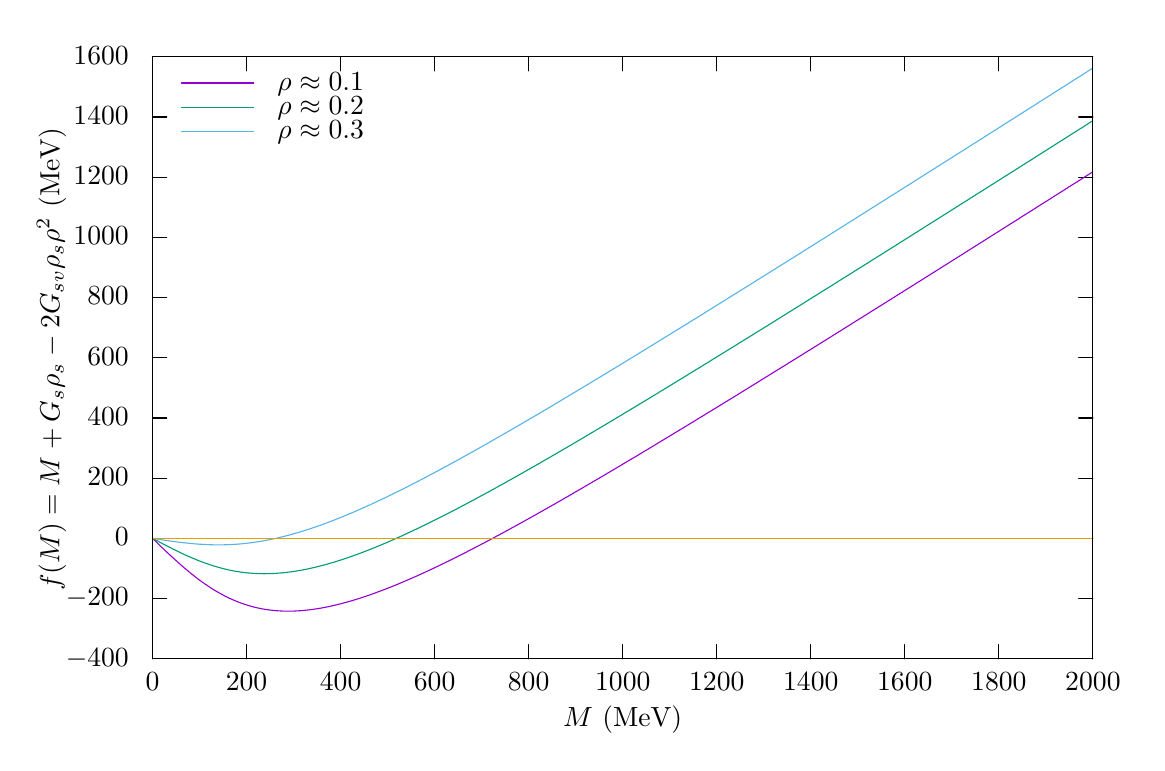
\begin{tikzpicture}[gnuplot]
%% generated with GNUPLOT 5.0p2 (Lua 5.2; terminal rev. 99, script rev. 100)
%% Thu Feb 25 17:15:55 2016
\path (0.000,0.000) rectangle (14.000,9.000);
\gpcolor{color=gp lt color border}
\gpsetlinetype{gp lt border}
\gpsetdashtype{gp dt solid}
\gpsetlinewidth{1.00}
\draw[gp path] (1.504,0.985)--(1.684,0.985);
\draw[gp path] (13.447,0.985)--(13.267,0.985);
\node[gp node right] at (1.320,0.985) {$-400$};
\draw[gp path] (1.504,1.750)--(1.684,1.750);
\draw[gp path] (13.447,1.750)--(13.267,1.750);
\node[gp node right] at (1.320,1.750) {$-200$};
\draw[gp path] (1.504,2.514)--(1.684,2.514);
\draw[gp path] (13.447,2.514)--(13.267,2.514);
\node[gp node right] at (1.320,2.514) {$0$};
\draw[gp path] (1.504,3.279)--(1.684,3.279);
\draw[gp path] (13.447,3.279)--(13.267,3.279);
\node[gp node right] at (1.320,3.279) {$200$};
\draw[gp path] (1.504,4.043)--(1.684,4.043);
\draw[gp path] (13.447,4.043)--(13.267,4.043);
\node[gp node right] at (1.320,4.043) {$400$};
\draw[gp path] (1.504,4.808)--(1.684,4.808);
\draw[gp path] (13.447,4.808)--(13.267,4.808);
\node[gp node right] at (1.320,4.808) {$600$};
\draw[gp path] (1.504,5.573)--(1.684,5.573);
\draw[gp path] (13.447,5.573)--(13.267,5.573);
\node[gp node right] at (1.320,5.573) {$800$};
\draw[gp path] (1.504,6.337)--(1.684,6.337);
\draw[gp path] (13.447,6.337)--(13.267,6.337);
\node[gp node right] at (1.320,6.337) {$1000$};
\draw[gp path] (1.504,7.102)--(1.684,7.102);
\draw[gp path] (13.447,7.102)--(13.267,7.102);
\node[gp node right] at (1.320,7.102) {$1200$};
\draw[gp path] (1.504,7.866)--(1.684,7.866);
\draw[gp path] (13.447,7.866)--(13.267,7.866);
\node[gp node right] at (1.320,7.866) {$1400$};
\draw[gp path] (1.504,8.631)--(1.684,8.631);
\draw[gp path] (13.447,8.631)--(13.267,8.631);
\node[gp node right] at (1.320,8.631) {$1600$};
\draw[gp path] (1.504,0.985)--(1.504,1.165);
\draw[gp path] (1.504,8.631)--(1.504,8.451);
\node[gp node center] at (1.504,0.677) {$0$};
\draw[gp path] (2.698,0.985)--(2.698,1.165);
\draw[gp path] (2.698,8.631)--(2.698,8.451);
\node[gp node center] at (2.698,0.677) {$200$};
\draw[gp path] (3.893,0.985)--(3.893,1.165);
\draw[gp path] (3.893,8.631)--(3.893,8.451);
\node[gp node center] at (3.893,0.677) {$400$};
\draw[gp path] (5.087,0.985)--(5.087,1.165);
\draw[gp path] (5.087,8.631)--(5.087,8.451);
\node[gp node center] at (5.087,0.677) {$600$};
\draw[gp path] (6.281,0.985)--(6.281,1.165);
\draw[gp path] (6.281,8.631)--(6.281,8.451);
\node[gp node center] at (6.281,0.677) {$800$};
\draw[gp path] (7.476,0.985)--(7.476,1.165);
\draw[gp path] (7.476,8.631)--(7.476,8.451);
\node[gp node center] at (7.476,0.677) {$1000$};
\draw[gp path] (8.670,0.985)--(8.670,1.165);
\draw[gp path] (8.670,8.631)--(8.670,8.451);
\node[gp node center] at (8.670,0.677) {$1200$};
\draw[gp path] (9.864,0.985)--(9.864,1.165);
\draw[gp path] (9.864,8.631)--(9.864,8.451);
\node[gp node center] at (9.864,0.677) {$1400$};
\draw[gp path] (11.058,0.985)--(11.058,1.165);
\draw[gp path] (11.058,8.631)--(11.058,8.451);
\node[gp node center] at (11.058,0.677) {$1600$};
\draw[gp path] (12.253,0.985)--(12.253,1.165);
\draw[gp path] (12.253,8.631)--(12.253,8.451);
\node[gp node center] at (12.253,0.677) {$1800$};
\draw[gp path] (13.447,0.985)--(13.447,1.165);
\draw[gp path] (13.447,8.631)--(13.447,8.451);
\node[gp node center] at (13.447,0.677) {$2000$};
\draw[gp path] (1.504,8.631)--(1.504,0.985)--(13.447,0.985)--(13.447,8.631)--cycle;
\node[gp node center,rotate=-270] at (0.246,4.808) {$f(M) = M + G_s\rho_s - 2G_{sv}\rho_s\rho^2$ (MeV)};
\node[gp node center] at (7.475,0.215) {$M$ (MeV)};
\node[gp node left] at (2.972,8.297) {$\rho \approx 0.1$};
\gpcolor{rgb color={0.580,0.000,0.827}}
\draw[gp path] (1.872,8.297)--(2.788,8.297);
\draw[gp path] (1.504,2.514)--(1.507,2.511)--(1.510,2.508)--(1.513,2.506)--(1.516,2.503)%
  --(1.519,2.500)--(1.522,2.497)--(1.525,2.494)--(1.528,2.491)--(1.531,2.488)--(1.534,2.485)%
  --(1.537,2.482)--(1.540,2.480)--(1.543,2.477)--(1.546,2.474)--(1.549,2.471)--(1.552,2.468)%
  --(1.555,2.465)--(1.558,2.462)--(1.561,2.459)--(1.564,2.457)--(1.567,2.454)--(1.570,2.451)%
  --(1.573,2.448)--(1.576,2.445)--(1.579,2.442)--(1.582,2.439)--(1.585,2.436)--(1.588,2.434)%
  --(1.591,2.431)--(1.594,2.428)--(1.597,2.425)--(1.600,2.422)--(1.603,2.419)--(1.606,2.416)%
  --(1.609,2.414)--(1.611,2.411)--(1.614,2.408)--(1.617,2.405)--(1.620,2.402)--(1.623,2.399)%
  --(1.626,2.396)--(1.629,2.394)--(1.632,2.391)--(1.635,2.388)--(1.638,2.385)--(1.641,2.382)%
  --(1.644,2.379)--(1.647,2.376)--(1.650,2.374)--(1.653,2.371)--(1.656,2.368)--(1.659,2.365)%
  --(1.662,2.362)--(1.665,2.359)--(1.668,2.357)--(1.671,2.354)--(1.674,2.351)--(1.677,2.348)%
  --(1.680,2.345)--(1.683,2.343)--(1.686,2.340)--(1.689,2.337)--(1.692,2.334)--(1.695,2.331)%
  --(1.698,2.328)--(1.701,2.326)--(1.704,2.323)--(1.707,2.320)--(1.710,2.317)--(1.713,2.314)%
  --(1.716,2.312)--(1.719,2.309)--(1.722,2.306)--(1.725,2.303)--(1.728,2.301)--(1.731,2.298)%
  --(1.734,2.295)--(1.737,2.292)--(1.740,2.289)--(1.743,2.287)--(1.746,2.284)--(1.749,2.281)%
  --(1.752,2.278)--(1.755,2.276)--(1.758,2.273)--(1.761,2.270)--(1.764,2.267)--(1.767,2.265)%
  --(1.770,2.262)--(1.773,2.259)--(1.776,2.256)--(1.779,2.254)--(1.782,2.251)--(1.785,2.248)%
  --(1.788,2.246)--(1.791,2.243)--(1.794,2.240)--(1.797,2.237)--(1.800,2.235)--(1.803,2.232)%
  --(1.806,2.229)--(1.809,2.227)--(1.812,2.224)--(1.815,2.221)--(1.818,2.219)--(1.820,2.216)%
  --(1.823,2.213)--(1.826,2.211)--(1.829,2.208)--(1.832,2.205)--(1.835,2.203)--(1.838,2.200)%
  --(1.841,2.197)--(1.844,2.195)--(1.847,2.192)--(1.850,2.189)--(1.853,2.187)--(1.856,2.184)%
  --(1.859,2.181)--(1.862,2.179)--(1.865,2.176)--(1.868,2.174)--(1.871,2.171)--(1.874,2.168)%
  --(1.877,2.166)--(1.880,2.163)--(1.883,2.161)--(1.886,2.158)--(1.889,2.155)--(1.892,2.153)%
  --(1.895,2.150)--(1.898,2.148)--(1.901,2.145)--(1.904,2.143)--(1.907,2.140)--(1.910,2.137)%
  --(1.913,2.135)--(1.916,2.132)--(1.919,2.130)--(1.922,2.127)--(1.925,2.125)--(1.928,2.122)%
  --(1.931,2.120)--(1.934,2.117)--(1.937,2.115)--(1.940,2.112)--(1.943,2.110)--(1.946,2.107)%
  --(1.949,2.105)--(1.952,2.102)--(1.955,2.100)--(1.958,2.097)--(1.961,2.095)--(1.964,2.092)%
  --(1.967,2.090)--(1.970,2.087)--(1.973,2.085)--(1.976,2.083)--(1.979,2.080)--(1.982,2.078)%
  --(1.985,2.075)--(1.988,2.073)--(1.991,2.070)--(1.994,2.068)--(1.997,2.066)--(2.000,2.063)%
  --(2.003,2.061)--(2.006,2.058)--(2.009,2.056)--(2.012,2.054)--(2.015,2.051)--(2.018,2.049)%
  --(2.021,2.046)--(2.024,2.044)--(2.027,2.042)--(2.029,2.039)--(2.032,2.037)--(2.035,2.035)%
  --(2.038,2.032)--(2.041,2.030)--(2.044,2.028)--(2.047,2.025)--(2.050,2.023)--(2.053,2.021)%
  --(2.056,2.018)--(2.059,2.016)--(2.062,2.014)--(2.065,2.012)--(2.068,2.009)--(2.071,2.007)%
  --(2.074,2.005)--(2.077,2.002)--(2.080,2.000)--(2.083,1.998)--(2.086,1.996)--(2.089,1.994)%
  --(2.092,1.991)--(2.095,1.989)--(2.098,1.987)--(2.101,1.985)--(2.104,1.982)--(2.107,1.980)%
  --(2.110,1.978)--(2.113,1.976)--(2.116,1.974)--(2.119,1.971)--(2.122,1.969)--(2.125,1.967)%
  --(2.128,1.965)--(2.131,1.963)--(2.134,1.961)--(2.137,1.958)--(2.140,1.956)--(2.143,1.954)%
  --(2.146,1.952)--(2.149,1.950)--(2.152,1.948)--(2.155,1.946)--(2.158,1.944)--(2.161,1.942)%
  --(2.164,1.939)--(2.167,1.937)--(2.170,1.935)--(2.173,1.933)--(2.176,1.931)--(2.179,1.929)%
  --(2.182,1.927)--(2.185,1.925)--(2.188,1.923)--(2.191,1.921)--(2.194,1.919)--(2.197,1.917)%
  --(2.200,1.915)--(2.203,1.913)--(2.206,1.911)--(2.209,1.909)--(2.212,1.907)--(2.215,1.905)%
  --(2.218,1.903)--(2.221,1.901)--(2.224,1.899)--(2.227,1.897)--(2.230,1.895)--(2.233,1.893)%
  --(2.236,1.891)--(2.238,1.889)--(2.241,1.887)--(2.244,1.885)--(2.247,1.883)--(2.250,1.882)%
  --(2.253,1.880)--(2.256,1.878)--(2.259,1.876)--(2.262,1.874)--(2.265,1.872)--(2.268,1.870)%
  --(2.271,1.868)--(2.274,1.867)--(2.277,1.865)--(2.280,1.863)--(2.283,1.861)--(2.286,1.859)%
  --(2.289,1.857)--(2.292,1.856)--(2.295,1.854)--(2.298,1.852)--(2.301,1.850)--(2.304,1.848)%
  --(2.307,1.847)--(2.310,1.845)--(2.313,1.843)--(2.316,1.841)--(2.319,1.839)--(2.322,1.838)%
  --(2.325,1.836)--(2.328,1.834)--(2.331,1.832)--(2.334,1.831)--(2.337,1.829)--(2.340,1.827)%
  --(2.343,1.826)--(2.346,1.824)--(2.349,1.822)--(2.352,1.821)--(2.355,1.819)--(2.358,1.817)%
  --(2.361,1.816)--(2.364,1.814)--(2.367,1.812)--(2.370,1.811)--(2.373,1.809)--(2.376,1.807)%
  --(2.379,1.806)--(2.382,1.804)--(2.385,1.802)--(2.388,1.801)--(2.391,1.799)--(2.394,1.798)%
  --(2.397,1.796)--(2.400,1.794)--(2.403,1.793)--(2.406,1.791)--(2.409,1.790)--(2.412,1.788)%
  --(2.415,1.787)--(2.418,1.785)--(2.421,1.784)--(2.424,1.782)--(2.427,1.780)--(2.430,1.779)%
  --(2.433,1.777)--(2.436,1.776)--(2.439,1.774)--(2.442,1.773)--(2.445,1.771)--(2.447,1.770)%
  --(2.450,1.768)--(2.453,1.767)--(2.456,1.766)--(2.459,1.764)--(2.462,1.763)--(2.465,1.761)%
  --(2.468,1.760)--(2.471,1.758)--(2.474,1.757)--(2.477,1.756)--(2.480,1.754)--(2.483,1.753)%
  --(2.486,1.751)--(2.489,1.750)--(2.492,1.749)--(2.495,1.747)--(2.498,1.746)--(2.501,1.744)%
  --(2.504,1.743)--(2.507,1.742)--(2.510,1.740)--(2.513,1.739)--(2.516,1.738)--(2.519,1.736)%
  --(2.522,1.735)--(2.525,1.734)--(2.528,1.732)--(2.531,1.731)--(2.534,1.730)--(2.537,1.729)%
  --(2.540,1.727)--(2.543,1.726)--(2.546,1.725)--(2.549,1.724)--(2.552,1.722)--(2.555,1.721)%
  --(2.558,1.720)--(2.561,1.719)--(2.564,1.717)--(2.567,1.716)--(2.570,1.715)--(2.573,1.714)%
  --(2.576,1.713)--(2.579,1.711)--(2.582,1.710)--(2.585,1.709)--(2.588,1.708)--(2.591,1.707)%
  --(2.594,1.705)--(2.597,1.704)--(2.600,1.703)--(2.603,1.702)--(2.606,1.701)--(2.609,1.700)%
  --(2.612,1.699)--(2.615,1.697)--(2.618,1.696)--(2.621,1.695)--(2.624,1.694)--(2.627,1.693)%
  --(2.630,1.692)--(2.633,1.691)--(2.636,1.690)--(2.639,1.689)--(2.642,1.688)--(2.645,1.687)%
  --(2.648,1.686)--(2.651,1.685)--(2.654,1.684)--(2.656,1.682)--(2.659,1.681)--(2.662,1.680)%
  --(2.665,1.679)--(2.668,1.678)--(2.671,1.677)--(2.674,1.676)--(2.677,1.675)--(2.680,1.674)%
  --(2.683,1.673)--(2.686,1.673)--(2.689,1.672)--(2.692,1.671)--(2.695,1.670)--(2.698,1.669)%
  --(2.701,1.668)--(2.704,1.667)--(2.707,1.666)--(2.710,1.665)--(2.713,1.664)--(2.716,1.663)%
  --(2.719,1.662)--(2.722,1.661)--(2.725,1.660)--(2.728,1.660)--(2.731,1.659)--(2.734,1.658)%
  --(2.737,1.657)--(2.740,1.656)--(2.743,1.655)--(2.746,1.654)--(2.749,1.654)--(2.752,1.653)%
  --(2.755,1.652)--(2.758,1.651)--(2.761,1.650)--(2.764,1.649)--(2.767,1.649)--(2.770,1.648)%
  --(2.773,1.647)--(2.776,1.646)--(2.779,1.646)--(2.782,1.645)--(2.785,1.644)--(2.788,1.643)%
  --(2.791,1.642)--(2.794,1.642)--(2.797,1.641)--(2.800,1.640)--(2.803,1.639)--(2.806,1.639)%
  --(2.809,1.638)--(2.812,1.637)--(2.815,1.637)--(2.818,1.636)--(2.821,1.635)--(2.824,1.635)%
  --(2.827,1.634)--(2.830,1.633)--(2.833,1.632)--(2.836,1.632)--(2.839,1.631)--(2.842,1.630)%
  --(2.845,1.630)--(2.848,1.629)--(2.851,1.629)--(2.854,1.628)--(2.857,1.627)--(2.860,1.627)%
  --(2.863,1.626)--(2.866,1.625)--(2.868,1.625)--(2.871,1.624)--(2.874,1.624)--(2.877,1.623)%
  --(2.880,1.622)--(2.883,1.622)--(2.886,1.621)--(2.889,1.621)--(2.892,1.620)--(2.895,1.620)%
  --(2.898,1.619)--(2.901,1.618)--(2.904,1.618)--(2.907,1.617)--(2.910,1.617)--(2.913,1.616)%
  --(2.916,1.616)--(2.919,1.615)--(2.922,1.615)--(2.925,1.614)--(2.928,1.614)--(2.931,1.613)%
  --(2.934,1.613)--(2.937,1.612)--(2.940,1.612)--(2.943,1.611)--(2.946,1.611)--(2.949,1.610)%
  --(2.952,1.610)--(2.955,1.610)--(2.958,1.609)--(2.961,1.609)--(2.964,1.608)--(2.967,1.608)%
  --(2.970,1.607)--(2.973,1.607)--(2.976,1.607)--(2.979,1.606)--(2.982,1.606)--(2.985,1.605)%
  --(2.988,1.605)--(2.991,1.605)--(2.994,1.604)--(2.997,1.604)--(3.000,1.603)--(3.003,1.603)%
  --(3.006,1.603)--(3.009,1.602)--(3.012,1.602)--(3.015,1.602)--(3.018,1.601)--(3.021,1.601)%
  --(3.024,1.601)--(3.027,1.600)--(3.030,1.600)--(3.033,1.600)--(3.036,1.599)--(3.039,1.599)%
  --(3.042,1.599)--(3.045,1.599)--(3.048,1.598)--(3.051,1.598)--(3.054,1.598)--(3.057,1.597)%
  --(3.060,1.597)--(3.063,1.597)--(3.066,1.597)--(3.069,1.596)--(3.072,1.596)--(3.075,1.596)%
  --(3.077,1.596)--(3.080,1.595)--(3.083,1.595)--(3.086,1.595)--(3.089,1.595)--(3.092,1.595)%
  --(3.095,1.594)--(3.098,1.594)--(3.101,1.594)--(3.104,1.594)--(3.107,1.594)--(3.110,1.593)%
  --(3.113,1.593)--(3.116,1.593)--(3.119,1.593)--(3.122,1.593)--(3.125,1.593)--(3.128,1.592)%
  --(3.131,1.592)--(3.134,1.592)--(3.137,1.592)--(3.140,1.592)--(3.143,1.592)--(3.146,1.592)%
  --(3.149,1.591)--(3.152,1.591)--(3.155,1.591)--(3.158,1.591)--(3.161,1.591)--(3.164,1.591)%
  --(3.167,1.591)--(3.170,1.591)--(3.173,1.591)--(3.176,1.591)--(3.179,1.590)--(3.182,1.590)%
  --(3.185,1.590)--(3.188,1.590)--(3.191,1.590)--(3.194,1.590)--(3.197,1.590)--(3.200,1.590)%
  --(3.203,1.590)--(3.206,1.590)--(3.209,1.590)--(3.212,1.590)--(3.215,1.590)--(3.218,1.590)%
  --(3.221,1.590)--(3.224,1.590)--(3.227,1.590)--(3.230,1.590)--(3.233,1.590)--(3.236,1.590)%
  --(3.239,1.590)--(3.242,1.590)--(3.245,1.590)--(3.248,1.590)--(3.251,1.590)--(3.254,1.590)%
  --(3.257,1.590)--(3.260,1.590)--(3.263,1.590)--(3.266,1.590)--(3.269,1.590)--(3.272,1.590)%
  --(3.275,1.590)--(3.278,1.591)--(3.281,1.591)--(3.284,1.591)--(3.286,1.591)--(3.289,1.591)%
  --(3.292,1.591)--(3.295,1.591)--(3.298,1.591)--(3.301,1.591)--(3.304,1.591)--(3.307,1.591)%
  --(3.310,1.592)--(3.313,1.592)--(3.316,1.592)--(3.319,1.592)--(3.322,1.592)--(3.325,1.592)%
  --(3.328,1.592)--(3.331,1.593)--(3.334,1.593)--(3.337,1.593)--(3.340,1.593)--(3.343,1.593)%
  --(3.346,1.593)--(3.349,1.593)--(3.352,1.594)--(3.355,1.594)--(3.358,1.594)--(3.361,1.594)%
  --(3.364,1.594)--(3.367,1.595)--(3.370,1.595)--(3.373,1.595)--(3.376,1.595)--(3.379,1.595)%
  --(3.382,1.596)--(3.385,1.596)--(3.388,1.596)--(3.391,1.596)--(3.394,1.597)--(3.397,1.597)%
  --(3.400,1.597)--(3.403,1.597)--(3.406,1.597)--(3.409,1.598)--(3.412,1.598)--(3.415,1.598)%
  --(3.418,1.599)--(3.421,1.599)--(3.424,1.599)--(3.427,1.599)--(3.430,1.600)--(3.433,1.600)%
  --(3.436,1.600)--(3.439,1.600)--(3.442,1.601)--(3.445,1.601)--(3.448,1.601)--(3.451,1.602)%
  --(3.454,1.602)--(3.457,1.602)--(3.460,1.603)--(3.463,1.603)--(3.466,1.603)--(3.469,1.604)%
  --(3.472,1.604)--(3.475,1.604)--(3.478,1.605)--(3.481,1.605)--(3.484,1.605)--(3.487,1.606)%
  --(3.490,1.606)--(3.493,1.606)--(3.495,1.607)--(3.498,1.607)--(3.501,1.607)--(3.504,1.608)%
  --(3.507,1.608)--(3.510,1.608)--(3.513,1.609)--(3.516,1.609)--(3.519,1.610)--(3.522,1.610)%
  --(3.525,1.610)--(3.528,1.611)--(3.531,1.611)--(3.534,1.612)--(3.537,1.612)--(3.540,1.612)%
  --(3.543,1.613)--(3.546,1.613)--(3.549,1.614)--(3.552,1.614)--(3.555,1.615)--(3.558,1.615)%
  --(3.561,1.615)--(3.564,1.616)--(3.567,1.616)--(3.570,1.617)--(3.573,1.617)--(3.576,1.618)%
  --(3.579,1.618)--(3.582,1.619)--(3.585,1.619)--(3.588,1.619)--(3.591,1.620)--(3.594,1.620)%
  --(3.597,1.621)--(3.600,1.621)--(3.603,1.622)--(3.606,1.622)--(3.609,1.623)--(3.612,1.623)%
  --(3.615,1.624)--(3.618,1.624)--(3.621,1.625)--(3.624,1.625)--(3.627,1.626)--(3.630,1.626)%
  --(3.633,1.627)--(3.636,1.627)--(3.639,1.628)--(3.642,1.628)--(3.645,1.629)--(3.648,1.630)%
  --(3.651,1.630)--(3.654,1.631)--(3.657,1.631)--(3.660,1.632)--(3.663,1.632)--(3.666,1.633)%
  --(3.669,1.633)--(3.672,1.634)--(3.675,1.634)--(3.678,1.635)--(3.681,1.636)--(3.684,1.636)%
  --(3.687,1.637)--(3.690,1.637)--(3.693,1.638)--(3.696,1.638)--(3.699,1.639)--(3.702,1.640)%
  --(3.704,1.640)--(3.707,1.641)--(3.710,1.641)--(3.713,1.642)--(3.716,1.643)--(3.719,1.643)%
  --(3.722,1.644)--(3.725,1.644)--(3.728,1.645)--(3.731,1.646)--(3.734,1.646)--(3.737,1.647)%
  --(3.740,1.647)--(3.743,1.648)--(3.746,1.649)--(3.749,1.649)--(3.752,1.650)--(3.755,1.651)%
  --(3.758,1.651)--(3.761,1.652)--(3.764,1.653)--(3.767,1.653)--(3.770,1.654)--(3.773,1.655)%
  --(3.776,1.655)--(3.779,1.656)--(3.782,1.657)--(3.785,1.657)--(3.788,1.658)--(3.791,1.659)%
  --(3.794,1.659)--(3.797,1.660)--(3.800,1.661)--(3.803,1.661)--(3.806,1.662)--(3.809,1.663)%
  --(3.812,1.663)--(3.815,1.664)--(3.818,1.665)--(3.821,1.665)--(3.824,1.666)--(3.827,1.667)%
  --(3.830,1.668)--(3.833,1.668)--(3.836,1.669)--(3.839,1.670)--(3.842,1.670)--(3.845,1.671)%
  --(3.848,1.672)--(3.851,1.673)--(3.854,1.673)--(3.857,1.674)--(3.860,1.675)--(3.863,1.676)%
  --(3.866,1.676)--(3.869,1.677)--(3.872,1.678)--(3.875,1.679)--(3.878,1.679)--(3.881,1.680)%
  --(3.884,1.681)--(3.887,1.682)--(3.890,1.682)--(3.893,1.683)--(3.896,1.684)--(3.899,1.685)%
  --(3.902,1.685)--(3.905,1.686)--(3.908,1.687)--(3.911,1.688)--(3.914,1.689)--(3.916,1.689)%
  --(3.919,1.690)--(3.922,1.691)--(3.925,1.692)--(3.928,1.693)--(3.931,1.693)--(3.934,1.694)%
  --(3.937,1.695)--(3.940,1.696)--(3.943,1.697)--(3.946,1.697)--(3.949,1.698)--(3.952,1.699)%
  --(3.955,1.700)--(3.958,1.701)--(3.961,1.701)--(3.964,1.702)--(3.967,1.703)--(3.970,1.704)%
  --(3.973,1.705)--(3.976,1.706)--(3.979,1.706)--(3.982,1.707)--(3.985,1.708)--(3.988,1.709)%
  --(3.991,1.710)--(3.994,1.711)--(3.997,1.712)--(4.000,1.712)--(4.003,1.713)--(4.006,1.714)%
  --(4.009,1.715)--(4.012,1.716)--(4.015,1.717)--(4.018,1.718)--(4.021,1.718)--(4.024,1.719)%
  --(4.027,1.720)--(4.030,1.721)--(4.033,1.722)--(4.036,1.723)--(4.039,1.724)--(4.042,1.725)%
  --(4.045,1.725)--(4.048,1.726)--(4.051,1.727)--(4.054,1.728)--(4.057,1.729)--(4.060,1.730)%
  --(4.063,1.731)--(4.066,1.732)--(4.069,1.733)--(4.072,1.734)--(4.075,1.735)--(4.078,1.735)%
  --(4.081,1.736)--(4.084,1.737)--(4.087,1.738)--(4.090,1.739)--(4.093,1.740)--(4.096,1.741)%
  --(4.099,1.742)--(4.102,1.743)--(4.105,1.744)--(4.108,1.745)--(4.111,1.746)--(4.114,1.747)%
  --(4.117,1.748)--(4.120,1.748)--(4.123,1.749)--(4.125,1.750)--(4.128,1.751)--(4.131,1.752)%
  --(4.134,1.753)--(4.137,1.754)--(4.140,1.755)--(4.143,1.756)--(4.146,1.757)--(4.149,1.758)%
  --(4.152,1.759)--(4.155,1.760)--(4.158,1.761)--(4.161,1.762)--(4.164,1.763)--(4.167,1.764)%
  --(4.170,1.765)--(4.173,1.766)--(4.176,1.767)--(4.179,1.768)--(4.182,1.769)--(4.185,1.770)%
  --(4.188,1.771)--(4.191,1.772)--(4.194,1.773)--(4.197,1.774)--(4.200,1.775)--(4.203,1.776)%
  --(4.206,1.777)--(4.209,1.778)--(4.212,1.779)--(4.215,1.780)--(4.218,1.781)--(4.221,1.782)%
  --(4.224,1.783)--(4.227,1.784)--(4.230,1.785)--(4.233,1.786)--(4.236,1.787)--(4.239,1.788)%
  --(4.242,1.789)--(4.245,1.790)--(4.248,1.791)--(4.251,1.792)--(4.254,1.793)--(4.257,1.794)%
  --(4.260,1.795)--(4.263,1.796)--(4.266,1.797)--(4.269,1.798)--(4.272,1.799)--(4.275,1.800)%
  --(4.278,1.801)--(4.281,1.802)--(4.284,1.804)--(4.287,1.805)--(4.290,1.806)--(4.293,1.807)%
  --(4.296,1.808)--(4.299,1.809)--(4.302,1.810)--(4.305,1.811)--(4.308,1.812)--(4.311,1.813)%
  --(4.314,1.814)--(4.317,1.815)--(4.320,1.816)--(4.323,1.817)--(4.326,1.818)--(4.329,1.820)%
  --(4.332,1.821)--(4.334,1.822)--(4.337,1.823)--(4.340,1.824)--(4.343,1.825)--(4.346,1.826)%
  --(4.349,1.827)--(4.352,1.828)--(4.355,1.829)--(4.358,1.830)--(4.361,1.832)--(4.364,1.833)%
  --(4.367,1.834)--(4.370,1.835)--(4.373,1.836)--(4.376,1.837)--(4.379,1.838)--(4.382,1.839)%
  --(4.385,1.840)--(4.388,1.842)--(4.391,1.843)--(4.394,1.844)--(4.397,1.845)--(4.400,1.846)%
  --(4.403,1.847)--(4.406,1.848)--(4.409,1.849)--(4.412,1.851)--(4.415,1.852)--(4.418,1.853)%
  --(4.421,1.854)--(4.424,1.855)--(4.427,1.856)--(4.430,1.857)--(4.433,1.858)--(4.436,1.860)%
  --(4.439,1.861)--(4.442,1.862)--(4.445,1.863)--(4.448,1.864)--(4.451,1.865)--(4.454,1.867)%
  --(4.457,1.868)--(4.460,1.869)--(4.463,1.870)--(4.466,1.871)--(4.469,1.872)--(4.472,1.873)%
  --(4.475,1.875)--(4.478,1.876)--(4.481,1.877)--(4.484,1.878)--(4.487,1.879)--(4.490,1.880)%
  --(4.493,1.882)--(4.496,1.883)--(4.499,1.884)--(4.502,1.885)--(4.505,1.886)--(4.508,1.888)%
  --(4.511,1.889)--(4.514,1.890)--(4.517,1.891)--(4.520,1.892)--(4.523,1.893)--(4.526,1.895)%
  --(4.529,1.896)--(4.532,1.897)--(4.535,1.898)--(4.538,1.899)--(4.541,1.901)--(4.543,1.902)%
  --(4.546,1.903)--(4.549,1.904)--(4.552,1.905)--(4.555,1.907)--(4.558,1.908)--(4.561,1.909)%
  --(4.564,1.910)--(4.567,1.911)--(4.570,1.913)--(4.573,1.914)--(4.576,1.915)--(4.579,1.916)%
  --(4.582,1.917)--(4.585,1.919)--(4.588,1.920)--(4.591,1.921)--(4.594,1.922)--(4.597,1.924)%
  --(4.600,1.925)--(4.603,1.926)--(4.606,1.927)--(4.609,1.929)--(4.612,1.930)--(4.615,1.931)%
  --(4.618,1.932)--(4.621,1.933)--(4.624,1.935)--(4.627,1.936)--(4.630,1.937)--(4.633,1.938)%
  --(4.636,1.940)--(4.639,1.941)--(4.642,1.942)--(4.645,1.943)--(4.648,1.945)--(4.651,1.946)%
  --(4.654,1.947)--(4.657,1.948)--(4.660,1.950)--(4.663,1.951)--(4.666,1.952)--(4.669,1.953)%
  --(4.672,1.955)--(4.675,1.956)--(4.678,1.957)--(4.681,1.958)--(4.684,1.960)--(4.687,1.961)%
  --(4.690,1.962)--(4.693,1.963)--(4.696,1.965)--(4.699,1.966)--(4.702,1.967)--(4.705,1.969)%
  --(4.708,1.970)--(4.711,1.971)--(4.714,1.972)--(4.717,1.974)--(4.720,1.975)--(4.723,1.976)%
  --(4.726,1.978)--(4.729,1.979)--(4.732,1.980)--(4.735,1.981)--(4.738,1.983)--(4.741,1.984)%
  --(4.744,1.985)--(4.747,1.987)--(4.750,1.988)--(4.752,1.989)--(4.755,1.990)--(4.758,1.992)%
  --(4.761,1.993)--(4.764,1.994)--(4.767,1.996)--(4.770,1.997)--(4.773,1.998)--(4.776,2.000)%
  --(4.779,2.001)--(4.782,2.002)--(4.785,2.003)--(4.788,2.005)--(4.791,2.006)--(4.794,2.007)%
  --(4.797,2.009)--(4.800,2.010)--(4.803,2.011)--(4.806,2.013)--(4.809,2.014)--(4.812,2.015)%
  --(4.815,2.017)--(4.818,2.018)--(4.821,2.019)--(4.824,2.021)--(4.827,2.022)--(4.830,2.023)%
  --(4.833,2.025)--(4.836,2.026)--(4.839,2.027)--(4.842,2.028)--(4.845,2.030)--(4.848,2.031)%
  --(4.851,2.032)--(4.854,2.034)--(4.857,2.035)--(4.860,2.036)--(4.863,2.038)--(4.866,2.039)%
  --(4.869,2.041)--(4.872,2.042)--(4.875,2.043)--(4.878,2.045)--(4.881,2.046)--(4.884,2.047)%
  --(4.887,2.049)--(4.890,2.050)--(4.893,2.051)--(4.896,2.053)--(4.899,2.054)--(4.902,2.055)%
  --(4.905,2.057)--(4.908,2.058)--(4.911,2.059)--(4.914,2.061)--(4.917,2.062)--(4.920,2.063)%
  --(4.923,2.065)--(4.926,2.066)--(4.929,2.068)--(4.932,2.069)--(4.935,2.070)--(4.938,2.072)%
  --(4.941,2.073)--(4.944,2.074)--(4.947,2.076)--(4.950,2.077)--(4.953,2.078)--(4.956,2.080)%
  --(4.959,2.081)--(4.961,2.083)--(4.964,2.084)--(4.967,2.085)--(4.970,2.087)--(4.973,2.088)%
  --(4.976,2.089)--(4.979,2.091)--(4.982,2.092)--(4.985,2.094)--(4.988,2.095)--(4.991,2.096)%
  --(4.994,2.098)--(4.997,2.099)--(5.000,2.101)--(5.003,2.102)--(5.006,2.103)--(5.009,2.105)%
  --(5.012,2.106)--(5.015,2.107)--(5.018,2.109)--(5.021,2.110)--(5.024,2.112)--(5.027,2.113)%
  --(5.030,2.114)--(5.033,2.116)--(5.036,2.117)--(5.039,2.119)--(5.042,2.120)--(5.045,2.121)%
  --(5.048,2.123)--(5.051,2.124)--(5.054,2.126)--(5.057,2.127)--(5.060,2.128)--(5.063,2.130)%
  --(5.066,2.131)--(5.069,2.133)--(5.072,2.134)--(5.075,2.136)--(5.078,2.137)--(5.081,2.138)%
  --(5.084,2.140)--(5.087,2.141)--(5.090,2.143)--(5.093,2.144)--(5.096,2.145)--(5.099,2.147)%
  --(5.102,2.148)--(5.105,2.150)--(5.108,2.151)--(5.111,2.153)--(5.114,2.154)--(5.117,2.155)%
  --(5.120,2.157)--(5.123,2.158)--(5.126,2.160)--(5.129,2.161)--(5.132,2.163)--(5.135,2.164)%
  --(5.138,2.165)--(5.141,2.167)--(5.144,2.168)--(5.147,2.170)--(5.150,2.171)--(5.153,2.173)%
  --(5.156,2.174)--(5.159,2.175)--(5.162,2.177)--(5.165,2.178)--(5.168,2.180)--(5.171,2.181)%
  --(5.173,2.183)--(5.176,2.184)--(5.179,2.186)--(5.182,2.187)--(5.185,2.188)--(5.188,2.190)%
  --(5.191,2.191)--(5.194,2.193)--(5.197,2.194)--(5.200,2.196)--(5.203,2.197)--(5.206,2.199)%
  --(5.209,2.200)--(5.212,2.201)--(5.215,2.203)--(5.218,2.204)--(5.221,2.206)--(5.224,2.207)%
  --(5.227,2.209)--(5.230,2.210)--(5.233,2.212)--(5.236,2.213)--(5.239,2.215)--(5.242,2.216)%
  --(5.245,2.218)--(5.248,2.219)--(5.251,2.220)--(5.254,2.222)--(5.257,2.223)--(5.260,2.225)%
  --(5.263,2.226)--(5.266,2.228)--(5.269,2.229)--(5.272,2.231)--(5.275,2.232)--(5.278,2.234)%
  --(5.281,2.235)--(5.284,2.237)--(5.287,2.238)--(5.290,2.240)--(5.293,2.241)--(5.296,2.243)%
  --(5.299,2.244)--(5.302,2.245)--(5.305,2.247)--(5.308,2.248)--(5.311,2.250)--(5.314,2.251)%
  --(5.317,2.253)--(5.320,2.254)--(5.323,2.256)--(5.326,2.257)--(5.329,2.259)--(5.332,2.260)%
  --(5.335,2.262)--(5.338,2.263)--(5.341,2.265)--(5.344,2.266)--(5.347,2.268)--(5.350,2.269)%
  --(5.353,2.271)--(5.356,2.272)--(5.359,2.274)--(5.362,2.275)--(5.365,2.277)--(5.368,2.278)%
  --(5.371,2.280)--(5.374,2.281)--(5.377,2.283)--(5.380,2.284)--(5.382,2.286)--(5.385,2.287)%
  --(5.388,2.289)--(5.391,2.290)--(5.394,2.292)--(5.397,2.293)--(5.400,2.295)--(5.403,2.296)%
  --(5.406,2.298)--(5.409,2.299)--(5.412,2.301)--(5.415,2.302)--(5.418,2.304)--(5.421,2.305)%
  --(5.424,2.307)--(5.427,2.308)--(5.430,2.310)--(5.433,2.311)--(5.436,2.313)--(5.439,2.314)%
  --(5.442,2.316)--(5.445,2.317)--(5.448,2.319)--(5.451,2.320)--(5.454,2.322)--(5.457,2.323)%
  --(5.460,2.325)--(5.463,2.326)--(5.466,2.328)--(5.469,2.329)--(5.472,2.331)--(5.475,2.333)%
  --(5.478,2.334)--(5.481,2.336)--(5.484,2.337)--(5.487,2.339)--(5.490,2.340)--(5.493,2.342)%
  --(5.496,2.343)--(5.499,2.345)--(5.502,2.346)--(5.505,2.348)--(5.508,2.349)--(5.511,2.351)%
  --(5.514,2.352)--(5.517,2.354)--(5.520,2.355)--(5.523,2.357)--(5.526,2.359)--(5.529,2.360)%
  --(5.532,2.362)--(5.535,2.363)--(5.538,2.365)--(5.541,2.366)--(5.544,2.368)--(5.547,2.369)%
  --(5.550,2.371)--(5.553,2.372)--(5.556,2.374)--(5.559,2.375)--(5.562,2.377)--(5.565,2.379)%
  --(5.568,2.380)--(5.571,2.382)--(5.574,2.383)--(5.577,2.385)--(5.580,2.386)--(5.583,2.388)%
  --(5.586,2.389)--(5.589,2.391)--(5.591,2.392)--(5.594,2.394)--(5.597,2.396)--(5.600,2.397)%
  --(5.603,2.399)--(5.606,2.400)--(5.609,2.402)--(5.612,2.403)--(5.615,2.405)--(5.618,2.406)%
  --(5.621,2.408)--(5.624,2.410)--(5.627,2.411)--(5.630,2.413)--(5.633,2.414)--(5.636,2.416)%
  --(5.639,2.417)--(5.642,2.419)--(5.645,2.420)--(5.648,2.422)--(5.651,2.424)--(5.654,2.425)%
  --(5.657,2.427)--(5.660,2.428)--(5.663,2.430)--(5.666,2.431)--(5.669,2.433)--(5.672,2.434)%
  --(5.675,2.436)--(5.678,2.438)--(5.681,2.439)--(5.684,2.441)--(5.687,2.442)--(5.690,2.444)%
  --(5.693,2.445)--(5.696,2.447)--(5.699,2.449)--(5.702,2.450)--(5.705,2.452)--(5.708,2.453)%
  --(5.711,2.455)--(5.714,2.456)--(5.717,2.458)--(5.720,2.460)--(5.723,2.461)--(5.726,2.463)%
  --(5.729,2.464)--(5.732,2.466)--(5.735,2.467)--(5.738,2.469)--(5.741,2.471)--(5.744,2.472)%
  --(5.747,2.474)--(5.750,2.475)--(5.753,2.477)--(5.756,2.479)--(5.759,2.480)--(5.762,2.482)%
  --(5.765,2.483)--(5.768,2.485)--(5.771,2.486)--(5.774,2.488)--(5.777,2.490)--(5.780,2.491)%
  --(5.783,2.493)--(5.786,2.494)--(5.789,2.496)--(5.792,2.498)--(5.795,2.499)--(5.798,2.501)%
  --(5.800,2.502)--(5.803,2.504)--(5.806,2.506)--(5.809,2.507)--(5.812,2.509)--(5.815,2.510)%
  --(5.818,2.512)--(5.821,2.513)--(5.824,2.515)--(5.827,2.517)--(5.830,2.518)--(5.833,2.520)%
  --(5.836,2.521)--(5.839,2.523)--(5.842,2.525)--(5.845,2.526)--(5.848,2.528)--(5.851,2.529)%
  --(5.854,2.531)--(5.857,2.533)--(5.860,2.534)--(5.863,2.536)--(5.866,2.537)--(5.869,2.539)%
  --(5.872,2.541)--(5.875,2.542)--(5.878,2.544)--(5.881,2.545)--(5.884,2.547)--(5.887,2.549)%
  --(5.890,2.550)--(5.893,2.552)--(5.896,2.554)--(5.899,2.555)--(5.902,2.557)--(5.905,2.558)%
  --(5.908,2.560)--(5.911,2.562)--(5.914,2.563)--(5.917,2.565)--(5.920,2.566)--(5.923,2.568)%
  --(5.926,2.570)--(5.929,2.571)--(5.932,2.573)--(5.935,2.574)--(5.938,2.576)--(5.941,2.578)%
  --(5.944,2.579)--(5.947,2.581)--(5.950,2.583)--(5.953,2.584)--(5.956,2.586)--(5.959,2.587)%
  --(5.962,2.589)--(5.965,2.591)--(5.968,2.592)--(5.971,2.594)--(5.974,2.595)--(5.977,2.597)%
  --(5.980,2.599)--(5.983,2.600)--(5.986,2.602)--(5.989,2.604)--(5.992,2.605)--(5.995,2.607)%
  --(5.998,2.608)--(6.001,2.610)--(6.004,2.612)--(6.007,2.613)--(6.009,2.615)--(6.012,2.617)%
  --(6.015,2.618)--(6.018,2.620)--(6.021,2.621)--(6.024,2.623)--(6.027,2.625)--(6.030,2.626)%
  --(6.033,2.628)--(6.036,2.630)--(6.039,2.631)--(6.042,2.633)--(6.045,2.635)--(6.048,2.636)%
  --(6.051,2.638)--(6.054,2.639)--(6.057,2.641)--(6.060,2.643)--(6.063,2.644)--(6.066,2.646)%
  --(6.069,2.648)--(6.072,2.649)--(6.075,2.651)--(6.078,2.652)--(6.081,2.654)--(6.084,2.656)%
  --(6.087,2.657)--(6.090,2.659)--(6.093,2.661)--(6.096,2.662)--(6.099,2.664)--(6.102,2.666)%
  --(6.105,2.667)--(6.108,2.669)--(6.111,2.671)--(6.114,2.672)--(6.117,2.674)--(6.120,2.675)%
  --(6.123,2.677)--(6.126,2.679)--(6.129,2.680)--(6.132,2.682)--(6.135,2.684)--(6.138,2.685)%
  --(6.141,2.687)--(6.144,2.689)--(6.147,2.690)--(6.150,2.692)--(6.153,2.694)--(6.156,2.695)%
  --(6.159,2.697)--(6.162,2.699)--(6.165,2.700)--(6.168,2.702)--(6.171,2.703)--(6.174,2.705)%
  --(6.177,2.707)--(6.180,2.708)--(6.183,2.710)--(6.186,2.712)--(6.189,2.713)--(6.192,2.715)%
  --(6.195,2.717)--(6.198,2.718)--(6.201,2.720)--(6.204,2.722)--(6.207,2.723)--(6.210,2.725)%
  --(6.213,2.727)--(6.216,2.728)--(6.218,2.730)--(6.221,2.732)--(6.224,2.733)--(6.227,2.735)%
  --(6.230,2.737)--(6.233,2.738)--(6.236,2.740)--(6.239,2.742)--(6.242,2.743)--(6.245,2.745)%
  --(6.248,2.747)--(6.251,2.748)--(6.254,2.750)--(6.257,2.751)--(6.260,2.753)--(6.263,2.755)%
  --(6.266,2.756)--(6.269,2.758)--(6.272,2.760)--(6.275,2.761)--(6.278,2.763)--(6.281,2.765)%
  --(6.284,2.766)--(6.287,2.768)--(6.290,2.770)--(6.293,2.771)--(6.296,2.773)--(6.299,2.775)%
  --(6.302,2.776)--(6.305,2.778)--(6.308,2.780)--(6.311,2.781)--(6.314,2.783)--(6.317,2.785)%
  --(6.320,2.786)--(6.323,2.788)--(6.326,2.790)--(6.329,2.792)--(6.332,2.793)--(6.335,2.795)%
  --(6.338,2.797)--(6.341,2.798)--(6.344,2.800)--(6.347,2.802)--(6.350,2.803)--(6.353,2.805)%
  --(6.356,2.807)--(6.359,2.808)--(6.362,2.810)--(6.365,2.812)--(6.368,2.813)--(6.371,2.815)%
  --(6.374,2.817)--(6.377,2.818)--(6.380,2.820)--(6.383,2.822)--(6.386,2.823)--(6.389,2.825)%
  --(6.392,2.827)--(6.395,2.828)--(6.398,2.830)--(6.401,2.832)--(6.404,2.833)--(6.407,2.835)%
  --(6.410,2.837)--(6.413,2.838)--(6.416,2.840)--(6.419,2.842)--(6.422,2.844)--(6.425,2.845)%
  --(6.428,2.847)--(6.430,2.849)--(6.433,2.850)--(6.436,2.852)--(6.439,2.854)--(6.442,2.855)%
  --(6.445,2.857)--(6.448,2.859)--(6.451,2.860)--(6.454,2.862)--(6.457,2.864)--(6.460,2.865)%
  --(6.463,2.867)--(6.466,2.869)--(6.469,2.870)--(6.472,2.872)--(6.475,2.874)--(6.478,2.876)%
  --(6.481,2.877)--(6.484,2.879)--(6.487,2.881)--(6.490,2.882)--(6.493,2.884)--(6.496,2.886)%
  --(6.499,2.887)--(6.502,2.889)--(6.505,2.891)--(6.508,2.892)--(6.511,2.894)--(6.514,2.896)%
  --(6.517,2.898)--(6.520,2.899)--(6.523,2.901)--(6.526,2.903)--(6.529,2.904)--(6.532,2.906)%
  --(6.535,2.908)--(6.538,2.909)--(6.541,2.911)--(6.544,2.913)--(6.547,2.915)--(6.550,2.916)%
  --(6.553,2.918)--(6.556,2.920)--(6.559,2.921)--(6.562,2.923)--(6.565,2.925)--(6.568,2.926)%
  --(6.571,2.928)--(6.574,2.930)--(6.577,2.932)--(6.580,2.933)--(6.583,2.935)--(6.586,2.937)%
  --(6.589,2.938)--(6.592,2.940)--(6.595,2.942)--(6.598,2.943)--(6.601,2.945)--(6.604,2.947)%
  --(6.607,2.949)--(6.610,2.950)--(6.613,2.952)--(6.616,2.954)--(6.619,2.955)--(6.622,2.957)%
  --(6.625,2.959)--(6.628,2.960)--(6.631,2.962)--(6.634,2.964)--(6.637,2.966)--(6.639,2.967)%
  --(6.642,2.969)--(6.645,2.971)--(6.648,2.972)--(6.651,2.974)--(6.654,2.976)--(6.657,2.978)%
  --(6.660,2.979)--(6.663,2.981)--(6.666,2.983)--(6.669,2.984)--(6.672,2.986)--(6.675,2.988)%
  --(6.678,2.990)--(6.681,2.991)--(6.684,2.993)--(6.687,2.995)--(6.690,2.996)--(6.693,2.998)%
  --(6.696,3.000)--(6.699,3.002)--(6.702,3.003)--(6.705,3.005)--(6.708,3.007)--(6.711,3.008)%
  --(6.714,3.010)--(6.717,3.012)--(6.720,3.014)--(6.723,3.015)--(6.726,3.017)--(6.729,3.019)%
  --(6.732,3.020)--(6.735,3.022)--(6.738,3.024)--(6.741,3.026)--(6.744,3.027)--(6.747,3.029)%
  --(6.750,3.031)--(6.753,3.032)--(6.756,3.034)--(6.759,3.036)--(6.762,3.038)--(6.765,3.039)%
  --(6.768,3.041)--(6.771,3.043)--(6.774,3.044)--(6.777,3.046)--(6.780,3.048)--(6.783,3.050)%
  --(6.786,3.051)--(6.789,3.053)--(6.792,3.055)--(6.795,3.056)--(6.798,3.058)--(6.801,3.060)%
  --(6.804,3.062)--(6.807,3.063)--(6.810,3.065)--(6.813,3.067)--(6.816,3.069)--(6.819,3.070)%
  --(6.822,3.072)--(6.825,3.074)--(6.828,3.075)--(6.831,3.077)--(6.834,3.079)--(6.837,3.081)%
  --(6.840,3.082)--(6.843,3.084)--(6.846,3.086)--(6.848,3.088)--(6.851,3.089)--(6.854,3.091)%
  --(6.857,3.093)--(6.860,3.094)--(6.863,3.096)--(6.866,3.098)--(6.869,3.100)--(6.872,3.101)%
  --(6.875,3.103)--(6.878,3.105)--(6.881,3.107)--(6.884,3.108)--(6.887,3.110)--(6.890,3.112)%
  --(6.893,3.114)--(6.896,3.115)--(6.899,3.117)--(6.902,3.119)--(6.905,3.120)--(6.908,3.122)%
  --(6.911,3.124)--(6.914,3.126)--(6.917,3.127)--(6.920,3.129)--(6.923,3.131)--(6.926,3.133)%
  --(6.929,3.134)--(6.932,3.136)--(6.935,3.138)--(6.938,3.140)--(6.941,3.141)--(6.944,3.143)%
  --(6.947,3.145)--(6.950,3.146)--(6.953,3.148)--(6.956,3.150)--(6.959,3.152)--(6.962,3.153)%
  --(6.965,3.155)--(6.968,3.157)--(6.971,3.159)--(6.974,3.160)--(6.977,3.162)--(6.980,3.164)%
  --(6.983,3.166)--(6.986,3.167)--(6.989,3.169)--(6.992,3.171)--(6.995,3.173)--(6.998,3.174)%
  --(7.001,3.176)--(7.004,3.178)--(7.007,3.179)--(7.010,3.181)--(7.013,3.183)--(7.016,3.185)%
  --(7.019,3.186)--(7.022,3.188)--(7.025,3.190)--(7.028,3.192)--(7.031,3.193)--(7.034,3.195)%
  --(7.037,3.197)--(7.040,3.199)--(7.043,3.200)--(7.046,3.202)--(7.049,3.204)--(7.052,3.206)%
  --(7.055,3.207)--(7.057,3.209)--(7.060,3.211)--(7.063,3.213)--(7.066,3.214)--(7.069,3.216)%
  --(7.072,3.218)--(7.075,3.220)--(7.078,3.221)--(7.081,3.223)--(7.084,3.225)--(7.087,3.227)%
  --(7.090,3.228)--(7.093,3.230)--(7.096,3.232)--(7.099,3.234)--(7.102,3.235)--(7.105,3.237)%
  --(7.108,3.239)--(7.111,3.241)--(7.114,3.242)--(7.117,3.244)--(7.120,3.246)--(7.123,3.248)%
  --(7.126,3.249)--(7.129,3.251)--(7.132,3.253)--(7.135,3.255)--(7.138,3.256)--(7.141,3.258)%
  --(7.144,3.260)--(7.147,3.262)--(7.150,3.263)--(7.153,3.265)--(7.156,3.267)--(7.159,3.269)%
  --(7.162,3.270)--(7.165,3.272)--(7.168,3.274)--(7.171,3.276)--(7.174,3.277)--(7.177,3.279)%
  --(7.180,3.281)--(7.183,3.283)--(7.186,3.284)--(7.189,3.286)--(7.192,3.288)--(7.195,3.290)%
  --(7.198,3.291)--(7.201,3.293)--(7.204,3.295)--(7.207,3.297)--(7.210,3.298)--(7.213,3.300)%
  --(7.216,3.302)--(7.219,3.304)--(7.222,3.305)--(7.225,3.307)--(7.228,3.309)--(7.231,3.311)%
  --(7.234,3.313)--(7.237,3.314)--(7.240,3.316)--(7.243,3.318)--(7.246,3.320)--(7.249,3.321)%
  --(7.252,3.323)--(7.255,3.325)--(7.258,3.327)--(7.261,3.328)--(7.264,3.330)--(7.266,3.332)%
  --(7.269,3.334)--(7.272,3.335)--(7.275,3.337)--(7.278,3.339)--(7.281,3.341)--(7.284,3.342)%
  --(7.287,3.344)--(7.290,3.346)--(7.293,3.348)--(7.296,3.350)--(7.299,3.351)--(7.302,3.353)%
  --(7.305,3.355)--(7.308,3.357)--(7.311,3.358)--(7.314,3.360)--(7.317,3.362)--(7.320,3.364)%
  --(7.323,3.365)--(7.326,3.367)--(7.329,3.369)--(7.332,3.371)--(7.335,3.372)--(7.338,3.374)%
  --(7.341,3.376)--(7.344,3.378)--(7.347,3.380)--(7.350,3.381)--(7.353,3.383)--(7.356,3.385)%
  --(7.359,3.387)--(7.362,3.388)--(7.365,3.390)--(7.368,3.392)--(7.371,3.394)--(7.374,3.395)%
  --(7.377,3.397)--(7.380,3.399)--(7.383,3.401)--(7.386,3.402)--(7.389,3.404)--(7.392,3.406)%
  --(7.395,3.408)--(7.398,3.410)--(7.401,3.411)--(7.404,3.413)--(7.407,3.415)--(7.410,3.417)%
  --(7.413,3.418)--(7.416,3.420)--(7.419,3.422)--(7.422,3.424)--(7.425,3.426)--(7.428,3.427)%
  --(7.431,3.429)--(7.434,3.431)--(7.437,3.433)--(7.440,3.434)--(7.443,3.436)--(7.446,3.438)%
  --(7.449,3.440)--(7.452,3.441)--(7.455,3.443)--(7.458,3.445)--(7.461,3.447)--(7.464,3.449)%
  --(7.467,3.450)--(7.470,3.452)--(7.473,3.454)--(7.476,3.456)--(7.478,3.457)--(7.481,3.459)%
  --(7.484,3.461)--(7.487,3.463)--(7.490,3.465)--(7.493,3.466)--(7.496,3.468)--(7.499,3.470)%
  --(7.502,3.472)--(7.505,3.473)--(7.508,3.475)--(7.511,3.477)--(7.514,3.479)--(7.517,3.481)%
  --(7.520,3.482)--(7.523,3.484)--(7.526,3.486)--(7.529,3.488)--(7.532,3.489)--(7.535,3.491)%
  --(7.538,3.493)--(7.541,3.495)--(7.544,3.497)--(7.547,3.498)--(7.550,3.500)--(7.553,3.502)%
  --(7.556,3.504)--(7.559,3.505)--(7.562,3.507)--(7.565,3.509)--(7.568,3.511)--(7.571,3.513)%
  --(7.574,3.514)--(7.577,3.516)--(7.580,3.518)--(7.583,3.520)--(7.586,3.521)--(7.589,3.523)%
  --(7.592,3.525)--(7.595,3.527)--(7.598,3.529)--(7.601,3.530)--(7.604,3.532)--(7.607,3.534)%
  --(7.610,3.536)--(7.613,3.537)--(7.616,3.539)--(7.619,3.541)--(7.622,3.543)--(7.625,3.545)%
  --(7.628,3.546)--(7.631,3.548)--(7.634,3.550)--(7.637,3.552)--(7.640,3.554)--(7.643,3.555)%
  --(7.646,3.557)--(7.649,3.559)--(7.652,3.561)--(7.655,3.562)--(7.658,3.564)--(7.661,3.566)%
  --(7.664,3.568)--(7.667,3.570)--(7.670,3.571)--(7.673,3.573)--(7.676,3.575)--(7.679,3.577)%
  --(7.682,3.579)--(7.685,3.580)--(7.687,3.582)--(7.690,3.584)--(7.693,3.586)--(7.696,3.587)%
  --(7.699,3.589)--(7.702,3.591)--(7.705,3.593)--(7.708,3.595)--(7.711,3.596)--(7.714,3.598)%
  --(7.717,3.600)--(7.720,3.602)--(7.723,3.604)--(7.726,3.605)--(7.729,3.607)--(7.732,3.609)%
  --(7.735,3.611)--(7.738,3.613)--(7.741,3.614)--(7.744,3.616)--(7.747,3.618)--(7.750,3.620)%
  --(7.753,3.621)--(7.756,3.623)--(7.759,3.625)--(7.762,3.627)--(7.765,3.629)--(7.768,3.630)%
  --(7.771,3.632)--(7.774,3.634)--(7.777,3.636)--(7.780,3.638)--(7.783,3.639)--(7.786,3.641)%
  --(7.789,3.643)--(7.792,3.645)--(7.795,3.647)--(7.798,3.648)--(7.801,3.650)--(7.804,3.652)%
  --(7.807,3.654)--(7.810,3.656)--(7.813,3.657)--(7.816,3.659)--(7.819,3.661)--(7.822,3.663)%
  --(7.825,3.664)--(7.828,3.666)--(7.831,3.668)--(7.834,3.670)--(7.837,3.672)--(7.840,3.673)%
  --(7.843,3.675)--(7.846,3.677)--(7.849,3.679)--(7.852,3.681)--(7.855,3.682)--(7.858,3.684)%
  --(7.861,3.686)--(7.864,3.688)--(7.867,3.690)--(7.870,3.691)--(7.873,3.693)--(7.876,3.695)%
  --(7.879,3.697)--(7.882,3.699)--(7.885,3.700)--(7.888,3.702)--(7.891,3.704)--(7.894,3.706)%
  --(7.896,3.708)--(7.899,3.709)--(7.902,3.711)--(7.905,3.713)--(7.908,3.715)--(7.911,3.717)%
  --(7.914,3.718)--(7.917,3.720)--(7.920,3.722)--(7.923,3.724)--(7.926,3.726)--(7.929,3.727)%
  --(7.932,3.729)--(7.935,3.731)--(7.938,3.733)--(7.941,3.735)--(7.944,3.736)--(7.947,3.738)%
  --(7.950,3.740)--(7.953,3.742)--(7.956,3.744)--(7.959,3.745)--(7.962,3.747)--(7.965,3.749)%
  --(7.968,3.751)--(7.971,3.753)--(7.974,3.754)--(7.977,3.756)--(7.980,3.758)--(7.983,3.760)%
  --(7.986,3.762)--(7.989,3.763)--(7.992,3.765)--(7.995,3.767)--(7.998,3.769)--(8.001,3.771)%
  --(8.004,3.772)--(8.007,3.774)--(8.010,3.776)--(8.013,3.778)--(8.016,3.780)--(8.019,3.781)%
  --(8.022,3.783)--(8.025,3.785)--(8.028,3.787)--(8.031,3.789)--(8.034,3.790)--(8.037,3.792)%
  --(8.040,3.794)--(8.043,3.796)--(8.046,3.798)--(8.049,3.799)--(8.052,3.801)--(8.055,3.803)%
  --(8.058,3.805)--(8.061,3.807)--(8.064,3.809)--(8.067,3.810)--(8.070,3.812)--(8.073,3.814)%
  --(8.076,3.816)--(8.079,3.818)--(8.082,3.819)--(8.085,3.821)--(8.088,3.823)--(8.091,3.825)%
  --(8.094,3.827)--(8.097,3.828)--(8.100,3.830)--(8.103,3.832)--(8.105,3.834)--(8.108,3.836)%
  --(8.111,3.837)--(8.114,3.839)--(8.117,3.841)--(8.120,3.843)--(8.123,3.845)--(8.126,3.846)%
  --(8.129,3.848)--(8.132,3.850)--(8.135,3.852)--(8.138,3.854)--(8.141,3.855)--(8.144,3.857)%
  --(8.147,3.859)--(8.150,3.861)--(8.153,3.863)--(8.156,3.865)--(8.159,3.866)--(8.162,3.868)%
  --(8.165,3.870)--(8.168,3.872)--(8.171,3.874)--(8.174,3.875)--(8.177,3.877)--(8.180,3.879)%
  --(8.183,3.881)--(8.186,3.883)--(8.189,3.884)--(8.192,3.886)--(8.195,3.888)--(8.198,3.890)%
  --(8.201,3.892)--(8.204,3.894)--(8.207,3.895)--(8.210,3.897)--(8.213,3.899)--(8.216,3.901)%
  --(8.219,3.903)--(8.222,3.904)--(8.225,3.906)--(8.228,3.908)--(8.231,3.910)--(8.234,3.912)%
  --(8.237,3.913)--(8.240,3.915)--(8.243,3.917)--(8.246,3.919)--(8.249,3.921)--(8.252,3.923)%
  --(8.255,3.924)--(8.258,3.926)--(8.261,3.928)--(8.264,3.930)--(8.267,3.932)--(8.270,3.933)%
  --(8.273,3.935)--(8.276,3.937)--(8.279,3.939)--(8.282,3.941)--(8.285,3.942)--(8.288,3.944)%
  --(8.291,3.946)--(8.294,3.948)--(8.297,3.950)--(8.300,3.952)--(8.303,3.953)--(8.306,3.955)%
  --(8.309,3.957)--(8.312,3.959)--(8.314,3.961)--(8.317,3.962)--(8.320,3.964)--(8.323,3.966)%
  --(8.326,3.968)--(8.329,3.970)--(8.332,3.972)--(8.335,3.973)--(8.338,3.975)--(8.341,3.977)%
  --(8.344,3.979)--(8.347,3.981)--(8.350,3.982)--(8.353,3.984)--(8.356,3.986)--(8.359,3.988)%
  --(8.362,3.990)--(8.365,3.992)--(8.368,3.993)--(8.371,3.995)--(8.374,3.997)--(8.377,3.999)%
  --(8.380,4.001)--(8.383,4.002)--(8.386,4.004)--(8.389,4.006)--(8.392,4.008)--(8.395,4.010)%
  --(8.398,4.012)--(8.401,4.013)--(8.404,4.015)--(8.407,4.017)--(8.410,4.019)--(8.413,4.021)%
  --(8.416,4.022)--(8.419,4.024)--(8.422,4.026)--(8.425,4.028)--(8.428,4.030)--(8.431,4.032)%
  --(8.434,4.033)--(8.437,4.035)--(8.440,4.037)--(8.443,4.039)--(8.446,4.041)--(8.449,4.042)%
  --(8.452,4.044)--(8.455,4.046)--(8.458,4.048)--(8.461,4.050)--(8.464,4.052)--(8.467,4.053)%
  --(8.470,4.055)--(8.473,4.057)--(8.476,4.059)--(8.479,4.061)--(8.482,4.063)--(8.485,4.064)%
  --(8.488,4.066)--(8.491,4.068)--(8.494,4.070)--(8.497,4.072)--(8.500,4.073)--(8.503,4.075)%
  --(8.506,4.077)--(8.509,4.079)--(8.512,4.081)--(8.515,4.083)--(8.518,4.084)--(8.521,4.086)%
  --(8.523,4.088)--(8.526,4.090)--(8.529,4.092)--(8.532,4.093)--(8.535,4.095)--(8.538,4.097)%
  --(8.541,4.099)--(8.544,4.101)--(8.547,4.103)--(8.550,4.104)--(8.553,4.106)--(8.556,4.108)%
  --(8.559,4.110)--(8.562,4.112)--(8.565,4.114)--(8.568,4.115)--(8.571,4.117)--(8.574,4.119)%
  --(8.577,4.121)--(8.580,4.123)--(8.583,4.125)--(8.586,4.126)--(8.589,4.128)--(8.592,4.130)%
  --(8.595,4.132)--(8.598,4.134)--(8.601,4.135)--(8.604,4.137)--(8.607,4.139)--(8.610,4.141)%
  --(8.613,4.143)--(8.616,4.145)--(8.619,4.146)--(8.622,4.148)--(8.625,4.150)--(8.628,4.152)%
  --(8.631,4.154)--(8.634,4.156)--(8.637,4.157)--(8.640,4.159)--(8.643,4.161)--(8.646,4.163)%
  --(8.649,4.165)--(8.652,4.167)--(8.655,4.168)--(8.658,4.170)--(8.661,4.172)--(8.664,4.174)%
  --(8.667,4.176)--(8.670,4.178)--(8.673,4.179)--(8.676,4.181)--(8.679,4.183)--(8.682,4.185)%
  --(8.685,4.187)--(8.688,4.188)--(8.691,4.190)--(8.694,4.192)--(8.697,4.194)--(8.700,4.196)%
  --(8.703,4.198)--(8.706,4.199)--(8.709,4.201)--(8.712,4.203)--(8.715,4.205)--(8.718,4.207)%
  --(8.721,4.209)--(8.724,4.210)--(8.727,4.212)--(8.730,4.214)--(8.733,4.216)--(8.735,4.218)%
  --(8.738,4.220)--(8.741,4.221)--(8.744,4.223)--(8.747,4.225)--(8.750,4.227)--(8.753,4.229)%
  --(8.756,4.231)--(8.759,4.232)--(8.762,4.234)--(8.765,4.236)--(8.768,4.238)--(8.771,4.240)%
  --(8.774,4.242)--(8.777,4.243)--(8.780,4.245)--(8.783,4.247)--(8.786,4.249)--(8.789,4.251)%
  --(8.792,4.253)--(8.795,4.254)--(8.798,4.256)--(8.801,4.258)--(8.804,4.260)--(8.807,4.262)%
  --(8.810,4.264)--(8.813,4.265)--(8.816,4.267)--(8.819,4.269)--(8.822,4.271)--(8.825,4.273)%
  --(8.828,4.275)--(8.831,4.276)--(8.834,4.278)--(8.837,4.280)--(8.840,4.282)--(8.843,4.284)%
  --(8.846,4.286)--(8.849,4.287)--(8.852,4.289)--(8.855,4.291)--(8.858,4.293)--(8.861,4.295)%
  --(8.864,4.297)--(8.867,4.298)--(8.870,4.300)--(8.873,4.302)--(8.876,4.304)--(8.879,4.306)%
  --(8.882,4.308)--(8.885,4.309)--(8.888,4.311)--(8.891,4.313)--(8.894,4.315)--(8.897,4.317)%
  --(8.900,4.319)--(8.903,4.320)--(8.906,4.322)--(8.909,4.324)--(8.912,4.326)--(8.915,4.328)%
  --(8.918,4.330)--(8.921,4.331)--(8.924,4.333)--(8.927,4.335)--(8.930,4.337)--(8.933,4.339)%
  --(8.936,4.341)--(8.939,4.342)--(8.942,4.344)--(8.944,4.346)--(8.947,4.348)--(8.950,4.350)%
  --(8.953,4.352)--(8.956,4.353)--(8.959,4.355)--(8.962,4.357)--(8.965,4.359)--(8.968,4.361)%
  --(8.971,4.363)--(8.974,4.365)--(8.977,4.366)--(8.980,4.368)--(8.983,4.370)--(8.986,4.372)%
  --(8.989,4.374)--(8.992,4.376)--(8.995,4.377)--(8.998,4.379)--(9.001,4.381)--(9.004,4.383)%
  --(9.007,4.385)--(9.010,4.387)--(9.013,4.388)--(9.016,4.390)--(9.019,4.392)--(9.022,4.394)%
  --(9.025,4.396)--(9.028,4.398)--(9.031,4.399)--(9.034,4.401)--(9.037,4.403)--(9.040,4.405)%
  --(9.043,4.407)--(9.046,4.409)--(9.049,4.410)--(9.052,4.412)--(9.055,4.414)--(9.058,4.416)%
  --(9.061,4.418)--(9.064,4.420)--(9.067,4.422)--(9.070,4.423)--(9.073,4.425)--(9.076,4.427)%
  --(9.079,4.429)--(9.082,4.431)--(9.085,4.433)--(9.088,4.434)--(9.091,4.436)--(9.094,4.438)%
  --(9.097,4.440)--(9.100,4.442)--(9.103,4.444)--(9.106,4.445)--(9.109,4.447)--(9.112,4.449)%
  --(9.115,4.451)--(9.118,4.453)--(9.121,4.455)--(9.124,4.456)--(9.127,4.458)--(9.130,4.460)%
  --(9.133,4.462)--(9.136,4.464)--(9.139,4.466)--(9.142,4.468)--(9.145,4.469)--(9.148,4.471)%
  --(9.151,4.473)--(9.153,4.475)--(9.156,4.477)--(9.159,4.479)--(9.162,4.480)--(9.165,4.482)%
  --(9.168,4.484)--(9.171,4.486)--(9.174,4.488)--(9.177,4.490)--(9.180,4.492)--(9.183,4.493)%
  --(9.186,4.495)--(9.189,4.497)--(9.192,4.499)--(9.195,4.501)--(9.198,4.503)--(9.201,4.504)%
  --(9.204,4.506)--(9.207,4.508)--(9.210,4.510)--(9.213,4.512)--(9.216,4.514)--(9.219,4.515)%
  --(9.222,4.517)--(9.225,4.519)--(9.228,4.521)--(9.231,4.523)--(9.234,4.525)--(9.237,4.527)%
  --(9.240,4.528)--(9.243,4.530)--(9.246,4.532)--(9.249,4.534)--(9.252,4.536)--(9.255,4.538)%
  --(9.258,4.539)--(9.261,4.541)--(9.264,4.543)--(9.267,4.545)--(9.270,4.547)--(9.273,4.549)%
  --(9.276,4.551)--(9.279,4.552)--(9.282,4.554)--(9.285,4.556)--(9.288,4.558)--(9.291,4.560)%
  --(9.294,4.562)--(9.297,4.563)--(9.300,4.565)--(9.303,4.567)--(9.306,4.569)--(9.309,4.571)%
  --(9.312,4.573)--(9.315,4.575)--(9.318,4.576)--(9.321,4.578)--(9.324,4.580)--(9.327,4.582)%
  --(9.330,4.584)--(9.333,4.586)--(9.336,4.587)--(9.339,4.589)--(9.342,4.591)--(9.345,4.593)%
  --(9.348,4.595)--(9.351,4.597)--(9.354,4.599)--(9.357,4.600)--(9.360,4.602)--(9.362,4.604)%
  --(9.365,4.606)--(9.368,4.608)--(9.371,4.610)--(9.374,4.611)--(9.377,4.613)--(9.380,4.615)%
  --(9.383,4.617)--(9.386,4.619)--(9.389,4.621)--(9.392,4.623)--(9.395,4.624)--(9.398,4.626)%
  --(9.401,4.628)--(9.404,4.630)--(9.407,4.632)--(9.410,4.634)--(9.413,4.635)--(9.416,4.637)%
  --(9.419,4.639)--(9.422,4.641)--(9.425,4.643)--(9.428,4.645)--(9.431,4.647)--(9.434,4.648)%
  --(9.437,4.650)--(9.440,4.652)--(9.443,4.654)--(9.446,4.656)--(9.449,4.658)--(9.452,4.660)%
  --(9.455,4.661)--(9.458,4.663)--(9.461,4.665)--(9.464,4.667)--(9.467,4.669)--(9.470,4.671)%
  --(9.473,4.672)--(9.476,4.674)--(9.479,4.676)--(9.482,4.678)--(9.485,4.680)--(9.488,4.682)%
  --(9.491,4.684)--(9.494,4.685)--(9.497,4.687)--(9.500,4.689)--(9.503,4.691)--(9.506,4.693)%
  --(9.509,4.695)--(9.512,4.697)--(9.515,4.698)--(9.518,4.700)--(9.521,4.702)--(9.524,4.704)%
  --(9.527,4.706)--(9.530,4.708)--(9.533,4.709)--(9.536,4.711)--(9.539,4.713)--(9.542,4.715)%
  --(9.545,4.717)--(9.548,4.719)--(9.551,4.721)--(9.554,4.722)--(9.557,4.724)--(9.560,4.726)%
  --(9.563,4.728)--(9.566,4.730)--(9.569,4.732)--(9.571,4.734)--(9.574,4.735)--(9.577,4.737)%
  --(9.580,4.739)--(9.583,4.741)--(9.586,4.743)--(9.589,4.745)--(9.592,4.747)--(9.595,4.748)%
  --(9.598,4.750)--(9.601,4.752)--(9.604,4.754)--(9.607,4.756)--(9.610,4.758)--(9.613,4.759)%
  --(9.616,4.761)--(9.619,4.763)--(9.622,4.765)--(9.625,4.767)--(9.628,4.769)--(9.631,4.771)%
  --(9.634,4.772)--(9.637,4.774)--(9.640,4.776)--(9.643,4.778)--(9.646,4.780)--(9.649,4.782)%
  --(9.652,4.784)--(9.655,4.785)--(9.658,4.787)--(9.661,4.789)--(9.664,4.791)--(9.667,4.793)%
  --(9.670,4.795)--(9.673,4.797)--(9.676,4.798)--(9.679,4.800)--(9.682,4.802)--(9.685,4.804)%
  --(9.688,4.806)--(9.691,4.808)--(9.694,4.810)--(9.697,4.811)--(9.700,4.813)--(9.703,4.815)%
  --(9.706,4.817)--(9.709,4.819)--(9.712,4.821)--(9.715,4.823)--(9.718,4.824)--(9.721,4.826)%
  --(9.724,4.828)--(9.727,4.830)--(9.730,4.832)--(9.733,4.834)--(9.736,4.836)--(9.739,4.837)%
  --(9.742,4.839)--(9.745,4.841)--(9.748,4.843)--(9.751,4.845)--(9.754,4.847)--(9.757,4.849)%
  --(9.760,4.850)--(9.763,4.852)--(9.766,4.854)--(9.769,4.856)--(9.772,4.858)--(9.775,4.860)%
  --(9.778,4.861)--(9.780,4.863)--(9.783,4.865)--(9.786,4.867)--(9.789,4.869)--(9.792,4.871)%
  --(9.795,4.873)--(9.798,4.874)--(9.801,4.876)--(9.804,4.878)--(9.807,4.880)--(9.810,4.882)%
  --(9.813,4.884)--(9.816,4.886)--(9.819,4.887)--(9.822,4.889)--(9.825,4.891)--(9.828,4.893)%
  --(9.831,4.895)--(9.834,4.897)--(9.837,4.899)--(9.840,4.900)--(9.843,4.902)--(9.846,4.904)%
  --(9.849,4.906)--(9.852,4.908)--(9.855,4.910)--(9.858,4.912)--(9.861,4.913)--(9.864,4.915)%
  --(9.867,4.917)--(9.870,4.919)--(9.873,4.921)--(9.876,4.923)--(9.879,4.925)--(9.882,4.926)%
  --(9.885,4.928)--(9.888,4.930)--(9.891,4.932)--(9.894,4.934)--(9.897,4.936)--(9.900,4.938)%
  --(9.903,4.940)--(9.906,4.941)--(9.909,4.943)--(9.912,4.945)--(9.915,4.947)--(9.918,4.949)%
  --(9.921,4.951)--(9.924,4.953)--(9.927,4.954)--(9.930,4.956)--(9.933,4.958)--(9.936,4.960)%
  --(9.939,4.962)--(9.942,4.964)--(9.945,4.966)--(9.948,4.967)--(9.951,4.969)--(9.954,4.971)%
  --(9.957,4.973)--(9.960,4.975)--(9.963,4.977)--(9.966,4.979)--(9.969,4.980)--(9.972,4.982)%
  --(9.975,4.984)--(9.978,4.986)--(9.981,4.988)--(9.984,4.990)--(9.987,4.992)--(9.990,4.993)%
  --(9.992,4.995)--(9.995,4.997)--(9.998,4.999)--(10.001,5.001)--(10.004,5.003)--(10.007,5.005)%
  --(10.010,5.006)--(10.013,5.008)--(10.016,5.010)--(10.019,5.012)--(10.022,5.014)--(10.025,5.016)%
  --(10.028,5.018)--(10.031,5.019)--(10.034,5.021)--(10.037,5.023)--(10.040,5.025)--(10.043,5.027)%
  --(10.046,5.029)--(10.049,5.031)--(10.052,5.032)--(10.055,5.034)--(10.058,5.036)--(10.061,5.038)%
  --(10.064,5.040)--(10.067,5.042)--(10.070,5.044)--(10.073,5.046)--(10.076,5.047)--(10.079,5.049)%
  --(10.082,5.051)--(10.085,5.053)--(10.088,5.055)--(10.091,5.057)--(10.094,5.059)--(10.097,5.060)%
  --(10.100,5.062)--(10.103,5.064)--(10.106,5.066)--(10.109,5.068)--(10.112,5.070)--(10.115,5.072)%
  --(10.118,5.073)--(10.121,5.075)--(10.124,5.077)--(10.127,5.079)--(10.130,5.081)--(10.133,5.083)%
  --(10.136,5.085)--(10.139,5.086)--(10.142,5.088)--(10.145,5.090)--(10.148,5.092)--(10.151,5.094)%
  --(10.154,5.096)--(10.157,5.098)--(10.160,5.100)--(10.163,5.101)--(10.166,5.103)--(10.169,5.105)%
  --(10.172,5.107)--(10.175,5.109)--(10.178,5.111)--(10.181,5.113)--(10.184,5.114)--(10.187,5.116)%
  --(10.190,5.118)--(10.193,5.120)--(10.196,5.122)--(10.199,5.124)--(10.201,5.126)--(10.204,5.127)%
  --(10.207,5.129)--(10.210,5.131)--(10.213,5.133)--(10.216,5.135)--(10.219,5.137)--(10.222,5.139)%
  --(10.225,5.141)--(10.228,5.142)--(10.231,5.144)--(10.234,5.146)--(10.237,5.148)--(10.240,5.150)%
  --(10.243,5.152)--(10.246,5.154)--(10.249,5.155)--(10.252,5.157)--(10.255,5.159)--(10.258,5.161)%
  --(10.261,5.163)--(10.264,5.165)--(10.267,5.167)--(10.270,5.168)--(10.273,5.170)--(10.276,5.172)%
  --(10.279,5.174)--(10.282,5.176)--(10.285,5.178)--(10.288,5.180)--(10.291,5.182)--(10.294,5.183)%
  --(10.297,5.185)--(10.300,5.187)--(10.303,5.189)--(10.306,5.191)--(10.309,5.193)--(10.312,5.195)%
  --(10.315,5.196)--(10.318,5.198)--(10.321,5.200)--(10.324,5.202)--(10.327,5.204)--(10.330,5.206)%
  --(10.333,5.208)--(10.336,5.210)--(10.339,5.211)--(10.342,5.213)--(10.345,5.215)--(10.348,5.217)%
  --(10.351,5.219)--(10.354,5.221)--(10.357,5.223)--(10.360,5.224)--(10.363,5.226)--(10.366,5.228)%
  --(10.369,5.230)--(10.372,5.232)--(10.375,5.234)--(10.378,5.236)--(10.381,5.237)--(10.384,5.239)%
  --(10.387,5.241)--(10.390,5.243)--(10.393,5.245)--(10.396,5.247)--(10.399,5.249)--(10.402,5.251)%
  --(10.405,5.252)--(10.408,5.254)--(10.410,5.256)--(10.413,5.258)--(10.416,5.260)--(10.419,5.262)%
  --(10.422,5.264)--(10.425,5.265)--(10.428,5.267)--(10.431,5.269)--(10.434,5.271)--(10.437,5.273)%
  --(10.440,5.275)--(10.443,5.277)--(10.446,5.279)--(10.449,5.280)--(10.452,5.282)--(10.455,5.284)%
  --(10.458,5.286)--(10.461,5.288)--(10.464,5.290)--(10.467,5.292)--(10.470,5.294)--(10.473,5.295)%
  --(10.476,5.297)--(10.479,5.299)--(10.482,5.301)--(10.485,5.303)--(10.488,5.305)--(10.491,5.307)%
  --(10.494,5.308)--(10.497,5.310)--(10.500,5.312)--(10.503,5.314)--(10.506,5.316)--(10.509,5.318)%
  --(10.512,5.320)--(10.515,5.322)--(10.518,5.323)--(10.521,5.325)--(10.524,5.327)--(10.527,5.329)%
  --(10.530,5.331)--(10.533,5.333)--(10.536,5.335)--(10.539,5.336)--(10.542,5.338)--(10.545,5.340)%
  --(10.548,5.342)--(10.551,5.344)--(10.554,5.346)--(10.557,5.348)--(10.560,5.350)--(10.563,5.351)%
  --(10.566,5.353)--(10.569,5.355)--(10.572,5.357)--(10.575,5.359)--(10.578,5.361)--(10.581,5.363)%
  --(10.584,5.364)--(10.587,5.366)--(10.590,5.368)--(10.593,5.370)--(10.596,5.372)--(10.599,5.374)%
  --(10.602,5.376)--(10.605,5.378)--(10.608,5.379)--(10.611,5.381)--(10.614,5.383)--(10.617,5.385)%
  --(10.619,5.387)--(10.622,5.389)--(10.625,5.391)--(10.628,5.393)--(10.631,5.394)--(10.634,5.396)%
  --(10.637,5.398)--(10.640,5.400)--(10.643,5.402)--(10.646,5.404)--(10.649,5.406)--(10.652,5.407)%
  --(10.655,5.409)--(10.658,5.411)--(10.661,5.413)--(10.664,5.415)--(10.667,5.417)--(10.670,5.419)%
  --(10.673,5.421)--(10.676,5.422)--(10.679,5.424)--(10.682,5.426)--(10.685,5.428)--(10.688,5.430)%
  --(10.691,5.432)--(10.694,5.434)--(10.697,5.436)--(10.700,5.437)--(10.703,5.439)--(10.706,5.441)%
  --(10.709,5.443)--(10.712,5.445)--(10.715,5.447)--(10.718,5.449)--(10.721,5.451)--(10.724,5.452)%
  --(10.727,5.454)--(10.730,5.456)--(10.733,5.458)--(10.736,5.460)--(10.739,5.462)--(10.742,5.464)%
  --(10.745,5.465)--(10.748,5.467)--(10.751,5.469)--(10.754,5.471)--(10.757,5.473)--(10.760,5.475)%
  --(10.763,5.477)--(10.766,5.479)--(10.769,5.480)--(10.772,5.482)--(10.775,5.484)--(10.778,5.486)%
  --(10.781,5.488)--(10.784,5.490)--(10.787,5.492)--(10.790,5.494)--(10.793,5.495)--(10.796,5.497)%
  --(10.799,5.499)--(10.802,5.501)--(10.805,5.503)--(10.808,5.505)--(10.811,5.507)--(10.814,5.509)%
  --(10.817,5.510)--(10.820,5.512)--(10.823,5.514)--(10.826,5.516)--(10.828,5.518)--(10.831,5.520)%
  --(10.834,5.522)--(10.837,5.524)--(10.840,5.525)--(10.843,5.527)--(10.846,5.529)--(10.849,5.531)%
  --(10.852,5.533)--(10.855,5.535)--(10.858,5.537)--(10.861,5.538)--(10.864,5.540)--(10.867,5.542)%
  --(10.870,5.544)--(10.873,5.546)--(10.876,5.548)--(10.879,5.550)--(10.882,5.552)--(10.885,5.553)%
  --(10.888,5.555)--(10.891,5.557)--(10.894,5.559)--(10.897,5.561)--(10.900,5.563)--(10.903,5.565)%
  --(10.906,5.567)--(10.909,5.568)--(10.912,5.570)--(10.915,5.572)--(10.918,5.574)--(10.921,5.576)%
  --(10.924,5.578)--(10.927,5.580)--(10.930,5.582)--(10.933,5.583)--(10.936,5.585)--(10.939,5.587)%
  --(10.942,5.589)--(10.945,5.591)--(10.948,5.593)--(10.951,5.595)--(10.954,5.597)--(10.957,5.598)%
  --(10.960,5.600)--(10.963,5.602)--(10.966,5.604)--(10.969,5.606)--(10.972,5.608)--(10.975,5.610)%
  --(10.978,5.612)--(10.981,5.613)--(10.984,5.615)--(10.987,5.617)--(10.990,5.619)--(10.993,5.621)%
  --(10.996,5.623)--(10.999,5.625)--(11.002,5.627)--(11.005,5.628)--(11.008,5.630)--(11.011,5.632)%
  --(11.014,5.634)--(11.017,5.636)--(11.020,5.638)--(11.023,5.640)--(11.026,5.642)--(11.029,5.643)%
  --(11.032,5.645)--(11.035,5.647)--(11.037,5.649)--(11.040,5.651)--(11.043,5.653)--(11.046,5.655)%
  --(11.049,5.657)--(11.052,5.658)--(11.055,5.660)--(11.058,5.662)--(11.061,5.664)--(11.064,5.666)%
  --(11.067,5.668)--(11.070,5.670)--(11.073,5.672)--(11.076,5.673)--(11.079,5.675)--(11.082,5.677)%
  --(11.085,5.679)--(11.088,5.681)--(11.091,5.683)--(11.094,5.685)--(11.097,5.687)--(11.100,5.688)%
  --(11.103,5.690)--(11.106,5.692)--(11.109,5.694)--(11.112,5.696)--(11.115,5.698)--(11.118,5.700)%
  --(11.121,5.702)--(11.124,5.703)--(11.127,5.705)--(11.130,5.707)--(11.133,5.709)--(11.136,5.711)%
  --(11.139,5.713)--(11.142,5.715)--(11.145,5.717)--(11.148,5.718)--(11.151,5.720)--(11.154,5.722)%
  --(11.157,5.724)--(11.160,5.726)--(11.163,5.728)--(11.166,5.730)--(11.169,5.732)--(11.172,5.733)%
  --(11.175,5.735)--(11.178,5.737)--(11.181,5.739)--(11.184,5.741)--(11.187,5.743)--(11.190,5.745)%
  --(11.193,5.747)--(11.196,5.748)--(11.199,5.750)--(11.202,5.752)--(11.205,5.754)--(11.208,5.756)%
  --(11.211,5.758)--(11.214,5.760)--(11.217,5.762)--(11.220,5.763)--(11.223,5.765)--(11.226,5.767)%
  --(11.229,5.769)--(11.232,5.771)--(11.235,5.773)--(11.238,5.775)--(11.241,5.777)--(11.244,5.778)%
  --(11.247,5.780)--(11.249,5.782)--(11.252,5.784)--(11.255,5.786)--(11.258,5.788)--(11.261,5.790)%
  --(11.264,5.792)--(11.267,5.793)--(11.270,5.795)--(11.273,5.797)--(11.276,5.799)--(11.279,5.801)%
  --(11.282,5.803)--(11.285,5.805)--(11.288,5.807)--(11.291,5.808)--(11.294,5.810)--(11.297,5.812)%
  --(11.300,5.814)--(11.303,5.816)--(11.306,5.818)--(11.309,5.820)--(11.312,5.822)--(11.315,5.823)%
  --(11.318,5.825)--(11.321,5.827)--(11.324,5.829)--(11.327,5.831)--(11.330,5.833)--(11.333,5.835)%
  --(11.336,5.837)--(11.339,5.839)--(11.342,5.840)--(11.345,5.842)--(11.348,5.844)--(11.351,5.846)%
  --(11.354,5.848)--(11.357,5.850)--(11.360,5.852)--(11.363,5.854)--(11.366,5.855)--(11.369,5.857)%
  --(11.372,5.859)--(11.375,5.861)--(11.378,5.863)--(11.381,5.865)--(11.384,5.867)--(11.387,5.869)%
  --(11.390,5.870)--(11.393,5.872)--(11.396,5.874)--(11.399,5.876)--(11.402,5.878)--(11.405,5.880)%
  --(11.408,5.882)--(11.411,5.884)--(11.414,5.885)--(11.417,5.887)--(11.420,5.889)--(11.423,5.891)%
  --(11.426,5.893)--(11.429,5.895)--(11.432,5.897)--(11.435,5.899)--(11.438,5.901)--(11.441,5.902)%
  --(11.444,5.904)--(11.447,5.906)--(11.450,5.908)--(11.453,5.910)--(11.456,5.912)--(11.458,5.914)%
  --(11.461,5.916)--(11.464,5.917)--(11.467,5.919)--(11.470,5.921)--(11.473,5.923)--(11.476,5.925)%
  --(11.479,5.927)--(11.482,5.929)--(11.485,5.931)--(11.488,5.932)--(11.491,5.934)--(11.494,5.936)%
  --(11.497,5.938)--(11.500,5.940)--(11.503,5.942)--(11.506,5.944)--(11.509,5.946)--(11.512,5.947)%
  --(11.515,5.949)--(11.518,5.951)--(11.521,5.953)--(11.524,5.955)--(11.527,5.957)--(11.530,5.959)%
  --(11.533,5.961)--(11.536,5.963)--(11.539,5.964)--(11.542,5.966)--(11.545,5.968)--(11.548,5.970)%
  --(11.551,5.972)--(11.554,5.974)--(11.557,5.976)--(11.560,5.978)--(11.563,5.979)--(11.566,5.981)%
  --(11.569,5.983)--(11.572,5.985)--(11.575,5.987)--(11.578,5.989)--(11.581,5.991)--(11.584,5.993)%
  --(11.587,5.994)--(11.590,5.996)--(11.593,5.998)--(11.596,6.000)--(11.599,6.002)--(11.602,6.004)%
  --(11.605,6.006)--(11.608,6.008)--(11.611,6.010)--(11.614,6.011)--(11.617,6.013)--(11.620,6.015)%
  --(11.623,6.017)--(11.626,6.019)--(11.629,6.021)--(11.632,6.023)--(11.635,6.025)--(11.638,6.026)%
  --(11.641,6.028)--(11.644,6.030)--(11.647,6.032)--(11.650,6.034)--(11.653,6.036)--(11.656,6.038)%
  --(11.659,6.040)--(11.662,6.041)--(11.665,6.043)--(11.667,6.045)--(11.670,6.047)--(11.673,6.049)%
  --(11.676,6.051)--(11.679,6.053)--(11.682,6.055)--(11.685,6.057)--(11.688,6.058)--(11.691,6.060)%
  --(11.694,6.062)--(11.697,6.064)--(11.700,6.066)--(11.703,6.068)--(11.706,6.070)--(11.709,6.072)%
  --(11.712,6.073)--(11.715,6.075)--(11.718,6.077)--(11.721,6.079)--(11.724,6.081)--(11.727,6.083)%
  --(11.730,6.085)--(11.733,6.087)--(11.736,6.089)--(11.739,6.090)--(11.742,6.092)--(11.745,6.094)%
  --(11.748,6.096)--(11.751,6.098)--(11.754,6.100)--(11.757,6.102)--(11.760,6.104)--(11.763,6.105)%
  --(11.766,6.107)--(11.769,6.109)--(11.772,6.111)--(11.775,6.113)--(11.778,6.115)--(11.781,6.117)%
  --(11.784,6.119)--(11.787,6.120)--(11.790,6.122)--(11.793,6.124)--(11.796,6.126)--(11.799,6.128)%
  --(11.802,6.130)--(11.805,6.132)--(11.808,6.134)--(11.811,6.136)--(11.814,6.137)--(11.817,6.139)%
  --(11.820,6.141)--(11.823,6.143)--(11.826,6.145)--(11.829,6.147)--(11.832,6.149)--(11.835,6.151)%
  --(11.838,6.152)--(11.841,6.154)--(11.844,6.156)--(11.847,6.158)--(11.850,6.160)--(11.853,6.162)%
  --(11.856,6.164)--(11.859,6.166)--(11.862,6.168)--(11.865,6.169)--(11.868,6.171)--(11.871,6.173)%
  --(11.874,6.175)--(11.876,6.177)--(11.879,6.179)--(11.882,6.181)--(11.885,6.183)--(11.888,6.184)%
  --(11.891,6.186)--(11.894,6.188)--(11.897,6.190)--(11.900,6.192)--(11.903,6.194)--(11.906,6.196)%
  --(11.909,6.198)--(11.912,6.200)--(11.915,6.201)--(11.918,6.203)--(11.921,6.205)--(11.924,6.207)%
  --(11.927,6.209)--(11.930,6.211)--(11.933,6.213)--(11.936,6.215)--(11.939,6.217)--(11.942,6.218)%
  --(11.945,6.220)--(11.948,6.222)--(11.951,6.224)--(11.954,6.226)--(11.957,6.228)--(11.960,6.230)%
  --(11.963,6.232)--(11.966,6.233)--(11.969,6.235)--(11.972,6.237)--(11.975,6.239)--(11.978,6.241)%
  --(11.981,6.243)--(11.984,6.245)--(11.987,6.247)--(11.990,6.249)--(11.993,6.250)--(11.996,6.252)%
  --(11.999,6.254)--(12.002,6.256)--(12.005,6.258)--(12.008,6.260)--(12.011,6.262)--(12.014,6.264)%
  --(12.017,6.265)--(12.020,6.267)--(12.023,6.269)--(12.026,6.271)--(12.029,6.273)--(12.032,6.275)%
  --(12.035,6.277)--(12.038,6.279)--(12.041,6.281)--(12.044,6.282)--(12.047,6.284)--(12.050,6.286)%
  --(12.053,6.288)--(12.056,6.290)--(12.059,6.292)--(12.062,6.294)--(12.065,6.296)--(12.068,6.297)%
  --(12.071,6.299)--(12.074,6.301)--(12.077,6.303)--(12.080,6.305)--(12.083,6.307)--(12.085,6.309)%
  --(12.088,6.311)--(12.091,6.313)--(12.094,6.314)--(12.097,6.316)--(12.100,6.318)--(12.103,6.320)%
  --(12.106,6.322)--(12.109,6.324)--(12.112,6.326)--(12.115,6.328)--(12.118,6.330)--(12.121,6.331)%
  --(12.124,6.333)--(12.127,6.335)--(12.130,6.337)--(12.133,6.339)--(12.136,6.341)--(12.139,6.343)%
  --(12.142,6.345)--(12.145,6.346)--(12.148,6.348)--(12.151,6.350)--(12.154,6.352)--(12.157,6.354)%
  --(12.160,6.356)--(12.163,6.358)--(12.166,6.360)--(12.169,6.362)--(12.172,6.363)--(12.175,6.365)%
  --(12.178,6.367)--(12.181,6.369)--(12.184,6.371)--(12.187,6.373)--(12.190,6.375)--(12.193,6.377)%
  --(12.196,6.379)--(12.199,6.380)--(12.202,6.382)--(12.205,6.384)--(12.208,6.386)--(12.211,6.388)%
  --(12.214,6.390)--(12.217,6.392)--(12.220,6.394)--(12.223,6.395)--(12.226,6.397)--(12.229,6.399)%
  --(12.232,6.401)--(12.235,6.403)--(12.238,6.405)--(12.241,6.407)--(12.244,6.409)--(12.247,6.411)%
  --(12.250,6.412)--(12.253,6.414)--(12.256,6.416)--(12.259,6.418)--(12.262,6.420)--(12.265,6.422)%
  --(12.268,6.424)--(12.271,6.426)--(12.274,6.428)--(12.277,6.429)--(12.280,6.431)--(12.283,6.433)%
  --(12.286,6.435)--(12.289,6.437)--(12.292,6.439)--(12.295,6.441)--(12.297,6.443)--(12.300,6.445)%
  --(12.303,6.446)--(12.306,6.448)--(12.309,6.450)--(12.312,6.452)--(12.315,6.454)--(12.318,6.456)%
  --(12.321,6.458)--(12.324,6.460)--(12.327,6.461)--(12.330,6.463)--(12.333,6.465)--(12.336,6.467)%
  --(12.339,6.469)--(12.342,6.471)--(12.345,6.473)--(12.348,6.475)--(12.351,6.477)--(12.354,6.478)%
  --(12.357,6.480)--(12.360,6.482)--(12.363,6.484)--(12.366,6.486)--(12.369,6.488)--(12.372,6.490)%
  --(12.375,6.492)--(12.378,6.494)--(12.381,6.495)--(12.384,6.497)--(12.387,6.499)--(12.390,6.501)%
  --(12.393,6.503)--(12.396,6.505)--(12.399,6.507)--(12.402,6.509)--(12.405,6.511)--(12.408,6.512)%
  --(12.411,6.514)--(12.414,6.516)--(12.417,6.518)--(12.420,6.520)--(12.423,6.522)--(12.426,6.524)%
  --(12.429,6.526)--(12.432,6.528)--(12.435,6.529)--(12.438,6.531)--(12.441,6.533)--(12.444,6.535)%
  --(12.447,6.537)--(12.450,6.539)--(12.453,6.541)--(12.456,6.543)--(12.459,6.544)--(12.462,6.546)%
  --(12.465,6.548)--(12.468,6.550)--(12.471,6.552)--(12.474,6.554)--(12.477,6.556)--(12.480,6.558)%
  --(12.483,6.560)--(12.486,6.561)--(12.489,6.563)--(12.492,6.565)--(12.495,6.567)--(12.498,6.569)%
  --(12.501,6.571)--(12.504,6.573)--(12.506,6.575)--(12.509,6.577)--(12.512,6.578)--(12.515,6.580)%
  --(12.518,6.582)--(12.521,6.584)--(12.524,6.586)--(12.527,6.588)--(12.530,6.590)--(12.533,6.592)%
  --(12.536,6.594)--(12.539,6.595)--(12.542,6.597)--(12.545,6.599)--(12.548,6.601)--(12.551,6.603)%
  --(12.554,6.605)--(12.557,6.607)--(12.560,6.609)--(12.563,6.611)--(12.566,6.612)--(12.569,6.614)%
  --(12.572,6.616)--(12.575,6.618)--(12.578,6.620)--(12.581,6.622)--(12.584,6.624)--(12.587,6.626)%
  --(12.590,6.628)--(12.593,6.629)--(12.596,6.631)--(12.599,6.633)--(12.602,6.635)--(12.605,6.637)%
  --(12.608,6.639)--(12.611,6.641)--(12.614,6.643)--(12.617,6.645)--(12.620,6.646)--(12.623,6.648)%
  --(12.626,6.650)--(12.629,6.652)--(12.632,6.654)--(12.635,6.656)--(12.638,6.658)--(12.641,6.660)%
  --(12.644,6.662)--(12.647,6.663)--(12.650,6.665)--(12.653,6.667)--(12.656,6.669)--(12.659,6.671)%
  --(12.662,6.673)--(12.665,6.675)--(12.668,6.677)--(12.671,6.678)--(12.674,6.680)--(12.677,6.682)%
  --(12.680,6.684)--(12.683,6.686)--(12.686,6.688)--(12.689,6.690)--(12.692,6.692)--(12.695,6.694)%
  --(12.698,6.695)--(12.701,6.697)--(12.704,6.699)--(12.707,6.701)--(12.710,6.703)--(12.713,6.705)%
  --(12.715,6.707)--(12.718,6.709)--(12.721,6.711)--(12.724,6.712)--(12.727,6.714)--(12.730,6.716)%
  --(12.733,6.718)--(12.736,6.720)--(12.739,6.722)--(12.742,6.724)--(12.745,6.726)--(12.748,6.728)%
  --(12.751,6.729)--(12.754,6.731)--(12.757,6.733)--(12.760,6.735)--(12.763,6.737)--(12.766,6.739)%
  --(12.769,6.741)--(12.772,6.743)--(12.775,6.745)--(12.778,6.746)--(12.781,6.748)--(12.784,6.750)%
  --(12.787,6.752)--(12.790,6.754)--(12.793,6.756)--(12.796,6.758)--(12.799,6.760)--(12.802,6.762)%
  --(12.805,6.763)--(12.808,6.765)--(12.811,6.767)--(12.814,6.769)--(12.817,6.771)--(12.820,6.773)%
  --(12.823,6.775)--(12.826,6.777)--(12.829,6.779)--(12.832,6.780)--(12.835,6.782)--(12.838,6.784)%
  --(12.841,6.786)--(12.844,6.788)--(12.847,6.790)--(12.850,6.792)--(12.853,6.794)--(12.856,6.796)%
  --(12.859,6.797)--(12.862,6.799)--(12.865,6.801)--(12.868,6.803)--(12.871,6.805)--(12.874,6.807)%
  --(12.877,6.809)--(12.880,6.811)--(12.883,6.813)--(12.886,6.814)--(12.889,6.816)--(12.892,6.818)%
  --(12.895,6.820)--(12.898,6.822)--(12.901,6.824)--(12.904,6.826)--(12.907,6.828)--(12.910,6.830)%
  --(12.913,6.831)--(12.916,6.833)--(12.919,6.835)--(12.922,6.837)--(12.924,6.839)--(12.927,6.841)%
  --(12.930,6.843)--(12.933,6.845)--(12.936,6.847)--(12.939,6.849)--(12.942,6.850)--(12.945,6.852)%
  --(12.948,6.854)--(12.951,6.856)--(12.954,6.858)--(12.957,6.860)--(12.960,6.862)--(12.963,6.864)%
  --(12.966,6.866)--(12.969,6.867)--(12.972,6.869)--(12.975,6.871)--(12.978,6.873)--(12.981,6.875)%
  --(12.984,6.877)--(12.987,6.879)--(12.990,6.881)--(12.993,6.883)--(12.996,6.884)--(12.999,6.886)%
  --(13.002,6.888)--(13.005,6.890)--(13.008,6.892)--(13.011,6.894)--(13.014,6.896)--(13.017,6.898)%
  --(13.020,6.900)--(13.023,6.901)--(13.026,6.903)--(13.029,6.905)--(13.032,6.907)--(13.035,6.909)%
  --(13.038,6.911)--(13.041,6.913)--(13.044,6.915)--(13.047,6.917)--(13.050,6.918)--(13.053,6.920)%
  --(13.056,6.922)--(13.059,6.924)--(13.062,6.926)--(13.065,6.928)--(13.068,6.930)--(13.071,6.932)%
  --(13.074,6.934)--(13.077,6.935)--(13.080,6.937)--(13.083,6.939)--(13.086,6.941)--(13.089,6.943)%
  --(13.092,6.945)--(13.095,6.947)--(13.098,6.949)--(13.101,6.951)--(13.104,6.952)--(13.107,6.954)%
  --(13.110,6.956)--(13.113,6.958)--(13.116,6.960)--(13.119,6.962)--(13.122,6.964)--(13.125,6.966)%
  --(13.128,6.968)--(13.131,6.969)--(13.133,6.971)--(13.136,6.973)--(13.139,6.975)--(13.142,6.977)%
  --(13.145,6.979)--(13.148,6.981)--(13.151,6.983)--(13.154,6.985)--(13.157,6.986)--(13.160,6.988)%
  --(13.163,6.990)--(13.166,6.992)--(13.169,6.994)--(13.172,6.996)--(13.175,6.998)--(13.178,7.000)%
  --(13.181,7.002)--(13.184,7.004)--(13.187,7.005)--(13.190,7.007)--(13.193,7.009)--(13.196,7.011)%
  --(13.199,7.013)--(13.202,7.015)--(13.205,7.017)--(13.208,7.019)--(13.211,7.021)--(13.214,7.022)%
  --(13.217,7.024)--(13.220,7.026)--(13.223,7.028)--(13.226,7.030)--(13.229,7.032)--(13.232,7.034)%
  --(13.235,7.036)--(13.238,7.038)--(13.241,7.039)--(13.244,7.041)--(13.247,7.043)--(13.250,7.045)%
  --(13.253,7.047)--(13.256,7.049)--(13.259,7.051)--(13.262,7.053)--(13.265,7.055)--(13.268,7.056)%
  --(13.271,7.058)--(13.274,7.060)--(13.277,7.062)--(13.280,7.064)--(13.283,7.066)--(13.286,7.068)%
  --(13.289,7.070)--(13.292,7.072)--(13.295,7.073)--(13.298,7.075)--(13.301,7.077)--(13.304,7.079)%
  --(13.307,7.081)--(13.310,7.083)--(13.313,7.085)--(13.316,7.087)--(13.319,7.089)--(13.322,7.091)%
  --(13.325,7.092)--(13.328,7.094)--(13.331,7.096)--(13.334,7.098)--(13.337,7.100)--(13.340,7.102)%
  --(13.342,7.104)--(13.345,7.106)--(13.348,7.108)--(13.351,7.109)--(13.354,7.111)--(13.357,7.113)%
  --(13.360,7.115)--(13.363,7.117)--(13.366,7.119)--(13.369,7.121)--(13.372,7.123)--(13.375,7.125)%
  --(13.378,7.126)--(13.381,7.128)--(13.384,7.130)--(13.387,7.132)--(13.390,7.134)--(13.393,7.136)%
  --(13.396,7.138)--(13.399,7.140)--(13.402,7.142)--(13.405,7.143)--(13.408,7.145)--(13.411,7.147)%
  --(13.414,7.149)--(13.417,7.151)--(13.420,7.153)--(13.423,7.155)--(13.426,7.157)--(13.429,7.159)%
  --(13.432,7.161)--(13.435,7.162)--(13.438,7.164)--(13.441,7.166)--(13.444,7.168);
\gpcolor{color=gp lt color border}
\node[gp node left] at (2.972,7.989) {$\rho \approx 0.2$};
\gpcolor{rgb color={0.000,0.620,0.451}}
\draw[gp path] (1.872,7.989)--(2.788,7.989);
\draw[gp path] (1.504,2.514)--(1.507,2.513)--(1.510,2.511)--(1.513,2.509)--(1.516,2.508)%
  --(1.519,2.506)--(1.522,2.505)--(1.525,2.503)--(1.528,2.502)--(1.531,2.500)--(1.534,2.498)%
  --(1.537,2.497)--(1.540,2.495)--(1.543,2.494)--(1.546,2.492)--(1.549,2.491)--(1.552,2.489)%
  --(1.555,2.487)--(1.558,2.486)--(1.561,2.484)--(1.564,2.483)--(1.567,2.481)--(1.570,2.479)%
  --(1.573,2.478)--(1.576,2.476)--(1.579,2.475)--(1.582,2.473)--(1.585,2.472)--(1.588,2.470)%
  --(1.591,2.468)--(1.594,2.467)--(1.597,2.465)--(1.600,2.464)--(1.603,2.462)--(1.606,2.461)%
  --(1.609,2.459)--(1.611,2.457)--(1.614,2.456)--(1.617,2.454)--(1.620,2.453)--(1.623,2.451)%
  --(1.626,2.450)--(1.629,2.448)--(1.632,2.447)--(1.635,2.445)--(1.638,2.443)--(1.641,2.442)%
  --(1.644,2.440)--(1.647,2.439)--(1.650,2.437)--(1.653,2.436)--(1.656,2.434)--(1.659,2.433)%
  --(1.662,2.431)--(1.665,2.429)--(1.668,2.428)--(1.671,2.426)--(1.674,2.425)--(1.677,2.423)%
  --(1.680,2.422)--(1.683,2.420)--(1.686,2.419)--(1.689,2.417)--(1.692,2.416)--(1.695,2.414)%
  --(1.698,2.413)--(1.701,2.411)--(1.704,2.409)--(1.707,2.408)--(1.710,2.406)--(1.713,2.405)%
  --(1.716,2.403)--(1.719,2.402)--(1.722,2.400)--(1.725,2.399)--(1.728,2.397)--(1.731,2.396)%
  --(1.734,2.394)--(1.737,2.393)--(1.740,2.391)--(1.743,2.390)--(1.746,2.388)--(1.749,2.387)%
  --(1.752,2.385)--(1.755,2.384)--(1.758,2.382)--(1.761,2.381)--(1.764,2.379)--(1.767,2.378)%
  --(1.770,2.376)--(1.773,2.375)--(1.776,2.373)--(1.779,2.372)--(1.782,2.370)--(1.785,2.369)%
  --(1.788,2.367)--(1.791,2.366)--(1.794,2.364)--(1.797,2.363)--(1.800,2.361)--(1.803,2.360)%
  --(1.806,2.358)--(1.809,2.357)--(1.812,2.356)--(1.815,2.354)--(1.818,2.353)--(1.820,2.351)%
  --(1.823,2.350)--(1.826,2.348)--(1.829,2.347)--(1.832,2.345)--(1.835,2.344)--(1.838,2.342)%
  --(1.841,2.341)--(1.844,2.340)--(1.847,2.338)--(1.850,2.337)--(1.853,2.335)--(1.856,2.334)%
  --(1.859,2.332)--(1.862,2.331)--(1.865,2.330)--(1.868,2.328)--(1.871,2.327)--(1.874,2.325)%
  --(1.877,2.324)--(1.880,2.323)--(1.883,2.321)--(1.886,2.320)--(1.889,2.318)--(1.892,2.317)%
  --(1.895,2.316)--(1.898,2.314)--(1.901,2.313)--(1.904,2.311)--(1.907,2.310)--(1.910,2.309)%
  --(1.913,2.307)--(1.916,2.306)--(1.919,2.305)--(1.922,2.303)--(1.925,2.302)--(1.928,2.300)%
  --(1.931,2.299)--(1.934,2.298)--(1.937,2.296)--(1.940,2.295)--(1.943,2.294)--(1.946,2.292)%
  --(1.949,2.291)--(1.952,2.290)--(1.955,2.288)--(1.958,2.287)--(1.961,2.286)--(1.964,2.284)%
  --(1.967,2.283)--(1.970,2.282)--(1.973,2.280)--(1.976,2.279)--(1.979,2.278)--(1.982,2.276)%
  --(1.985,2.275)--(1.988,2.274)--(1.991,2.273)--(1.994,2.271)--(1.997,2.270)--(2.000,2.269)%
  --(2.003,2.267)--(2.006,2.266)--(2.009,2.265)--(2.012,2.264)--(2.015,2.262)--(2.018,2.261)%
  --(2.021,2.260)--(2.024,2.259)--(2.027,2.257)--(2.029,2.256)--(2.032,2.255)--(2.035,2.254)%
  --(2.038,2.252)--(2.041,2.251)--(2.044,2.250)--(2.047,2.249)--(2.050,2.247)--(2.053,2.246)%
  --(2.056,2.245)--(2.059,2.244)--(2.062,2.242)--(2.065,2.241)--(2.068,2.240)--(2.071,2.239)%
  --(2.074,2.238)--(2.077,2.236)--(2.080,2.235)--(2.083,2.234)--(2.086,2.233)--(2.089,2.232)%
  --(2.092,2.231)--(2.095,2.229)--(2.098,2.228)--(2.101,2.227)--(2.104,2.226)--(2.107,2.225)%
  --(2.110,2.224)--(2.113,2.222)--(2.116,2.221)--(2.119,2.220)--(2.122,2.219)--(2.125,2.218)%
  --(2.128,2.217)--(2.131,2.216)--(2.134,2.214)--(2.137,2.213)--(2.140,2.212)--(2.143,2.211)%
  --(2.146,2.210)--(2.149,2.209)--(2.152,2.208)--(2.155,2.207)--(2.158,2.206)--(2.161,2.204)%
  --(2.164,2.203)--(2.167,2.202)--(2.170,2.201)--(2.173,2.200)--(2.176,2.199)--(2.179,2.198)%
  --(2.182,2.197)--(2.185,2.196)--(2.188,2.195)--(2.191,2.194)--(2.194,2.193)--(2.197,2.192)%
  --(2.200,2.191)--(2.203,2.190)--(2.206,2.189)--(2.209,2.188)--(2.212,2.187)--(2.215,2.186)%
  --(2.218,2.184)--(2.221,2.183)--(2.224,2.182)--(2.227,2.181)--(2.230,2.180)--(2.233,2.179)%
  --(2.236,2.178)--(2.238,2.178)--(2.241,2.177)--(2.244,2.176)--(2.247,2.175)--(2.250,2.174)%
  --(2.253,2.173)--(2.256,2.172)--(2.259,2.171)--(2.262,2.170)--(2.265,2.169)--(2.268,2.168)%
  --(2.271,2.167)--(2.274,2.166)--(2.277,2.165)--(2.280,2.164)--(2.283,2.163)--(2.286,2.162)%
  --(2.289,2.161)--(2.292,2.160)--(2.295,2.160)--(2.298,2.159)--(2.301,2.158)--(2.304,2.157)%
  --(2.307,2.156)--(2.310,2.155)--(2.313,2.154)--(2.316,2.153)--(2.319,2.152)--(2.322,2.152)%
  --(2.325,2.151)--(2.328,2.150)--(2.331,2.149)--(2.334,2.148)--(2.337,2.147)--(2.340,2.146)%
  --(2.343,2.146)--(2.346,2.145)--(2.349,2.144)--(2.352,2.143)--(2.355,2.142)--(2.358,2.142)%
  --(2.361,2.141)--(2.364,2.140)--(2.367,2.139)--(2.370,2.138)--(2.373,2.138)--(2.376,2.137)%
  --(2.379,2.136)--(2.382,2.135)--(2.385,2.134)--(2.388,2.134)--(2.391,2.133)--(2.394,2.132)%
  --(2.397,2.131)--(2.400,2.131)--(2.403,2.130)--(2.406,2.129)--(2.409,2.128)--(2.412,2.128)%
  --(2.415,2.127)--(2.418,2.126)--(2.421,2.125)--(2.424,2.125)--(2.427,2.124)--(2.430,2.123)%
  --(2.433,2.123)--(2.436,2.122)--(2.439,2.121)--(2.442,2.120)--(2.445,2.120)--(2.447,2.119)%
  --(2.450,2.118)--(2.453,2.118)--(2.456,2.117)--(2.459,2.116)--(2.462,2.116)--(2.465,2.115)%
  --(2.468,2.114)--(2.471,2.114)--(2.474,2.113)--(2.477,2.112)--(2.480,2.112)--(2.483,2.111)%
  --(2.486,2.111)--(2.489,2.110)--(2.492,2.109)--(2.495,2.109)--(2.498,2.108)--(2.501,2.108)%
  --(2.504,2.107)--(2.507,2.106)--(2.510,2.106)--(2.513,2.105)--(2.516,2.105)--(2.519,2.104)%
  --(2.522,2.103)--(2.525,2.103)--(2.528,2.102)--(2.531,2.102)--(2.534,2.101)--(2.537,2.101)%
  --(2.540,2.100)--(2.543,2.099)--(2.546,2.099)--(2.549,2.098)--(2.552,2.098)--(2.555,2.097)%
  --(2.558,2.097)--(2.561,2.096)--(2.564,2.096)--(2.567,2.095)--(2.570,2.095)--(2.573,2.094)%
  --(2.576,2.094)--(2.579,2.093)--(2.582,2.093)--(2.585,2.092)--(2.588,2.092)--(2.591,2.091)%
  --(2.594,2.091)--(2.597,2.090)--(2.600,2.090)--(2.603,2.090)--(2.606,2.089)--(2.609,2.089)%
  --(2.612,2.088)--(2.615,2.088)--(2.618,2.087)--(2.621,2.087)--(2.624,2.086)--(2.627,2.086)%
  --(2.630,2.086)--(2.633,2.085)--(2.636,2.085)--(2.639,2.084)--(2.642,2.084)--(2.645,2.084)%
  --(2.648,2.083)--(2.651,2.083)--(2.654,2.082)--(2.656,2.082)--(2.659,2.082)--(2.662,2.081)%
  --(2.665,2.081)--(2.668,2.081)--(2.671,2.080)--(2.674,2.080)--(2.677,2.080)--(2.680,2.079)%
  --(2.683,2.079)--(2.686,2.079)--(2.689,2.078)--(2.692,2.078)--(2.695,2.078)--(2.698,2.077)%
  --(2.701,2.077)--(2.704,2.077)--(2.707,2.076)--(2.710,2.076)--(2.713,2.076)--(2.716,2.075)%
  --(2.719,2.075)--(2.722,2.075)--(2.725,2.075)--(2.728,2.074)--(2.731,2.074)--(2.734,2.074)%
  --(2.737,2.074)--(2.740,2.073)--(2.743,2.073)--(2.746,2.073)--(2.749,2.073)--(2.752,2.072)%
  --(2.755,2.072)--(2.758,2.072)--(2.761,2.072)--(2.764,2.071)--(2.767,2.071)--(2.770,2.071)%
  --(2.773,2.071)--(2.776,2.071)--(2.779,2.070)--(2.782,2.070)--(2.785,2.070)--(2.788,2.070)%
  --(2.791,2.070)--(2.794,2.069)--(2.797,2.069)--(2.800,2.069)--(2.803,2.069)--(2.806,2.069)%
  --(2.809,2.069)--(2.812,2.068)--(2.815,2.068)--(2.818,2.068)--(2.821,2.068)--(2.824,2.068)%
  --(2.827,2.068)--(2.830,2.068)--(2.833,2.067)--(2.836,2.067)--(2.839,2.067)--(2.842,2.067)%
  --(2.845,2.067)--(2.848,2.067)--(2.851,2.067)--(2.854,2.067)--(2.857,2.067)--(2.860,2.066)%
  --(2.863,2.066)--(2.866,2.066)--(2.868,2.066)--(2.871,2.066)--(2.874,2.066)--(2.877,2.066)%
  --(2.880,2.066)--(2.883,2.066)--(2.886,2.066)--(2.889,2.066)--(2.892,2.066)--(2.895,2.066)%
  --(2.898,2.066)--(2.901,2.066)--(2.904,2.066)--(2.907,2.066)--(2.910,2.066)--(2.913,2.066)%
  --(2.916,2.065)--(2.919,2.065)--(2.922,2.065)--(2.925,2.065)--(2.928,2.065)--(2.931,2.065)%
  --(2.934,2.065)--(2.937,2.066)--(2.940,2.066)--(2.943,2.066)--(2.946,2.066)--(2.949,2.066)%
  --(2.952,2.066)--(2.955,2.066)--(2.958,2.066)--(2.961,2.066)--(2.964,2.066)--(2.967,2.066)%
  --(2.970,2.066)--(2.973,2.066)--(2.976,2.066)--(2.979,2.066)--(2.982,2.066)--(2.985,2.066)%
  --(2.988,2.066)--(2.991,2.066)--(2.994,2.067)--(2.997,2.067)--(3.000,2.067)--(3.003,2.067)%
  --(3.006,2.067)--(3.009,2.067)--(3.012,2.067)--(3.015,2.067)--(3.018,2.067)--(3.021,2.067)%
  --(3.024,2.068)--(3.027,2.068)--(3.030,2.068)--(3.033,2.068)--(3.036,2.068)--(3.039,2.068)%
  --(3.042,2.068)--(3.045,2.069)--(3.048,2.069)--(3.051,2.069)--(3.054,2.069)--(3.057,2.069)%
  --(3.060,2.069)--(3.063,2.070)--(3.066,2.070)--(3.069,2.070)--(3.072,2.070)--(3.075,2.070)%
  --(3.077,2.070)--(3.080,2.071)--(3.083,2.071)--(3.086,2.071)--(3.089,2.071)--(3.092,2.072)%
  --(3.095,2.072)--(3.098,2.072)--(3.101,2.072)--(3.104,2.072)--(3.107,2.073)--(3.110,2.073)%
  --(3.113,2.073)--(3.116,2.073)--(3.119,2.074)--(3.122,2.074)--(3.125,2.074)--(3.128,2.074)%
  --(3.131,2.075)--(3.134,2.075)--(3.137,2.075)--(3.140,2.075)--(3.143,2.076)--(3.146,2.076)%
  --(3.149,2.076)--(3.152,2.076)--(3.155,2.077)--(3.158,2.077)--(3.161,2.077)--(3.164,2.078)%
  --(3.167,2.078)--(3.170,2.078)--(3.173,2.079)--(3.176,2.079)--(3.179,2.079)--(3.182,2.079)%
  --(3.185,2.080)--(3.188,2.080)--(3.191,2.080)--(3.194,2.081)--(3.197,2.081)--(3.200,2.081)%
  --(3.203,2.082)--(3.206,2.082)--(3.209,2.082)--(3.212,2.083)--(3.215,2.083)--(3.218,2.084)%
  --(3.221,2.084)--(3.224,2.084)--(3.227,2.085)--(3.230,2.085)--(3.233,2.085)--(3.236,2.086)%
  --(3.239,2.086)--(3.242,2.087)--(3.245,2.087)--(3.248,2.087)--(3.251,2.088)--(3.254,2.088)%
  --(3.257,2.089)--(3.260,2.089)--(3.263,2.089)--(3.266,2.090)--(3.269,2.090)--(3.272,2.091)%
  --(3.275,2.091)--(3.278,2.091)--(3.281,2.092)--(3.284,2.092)--(3.286,2.093)--(3.289,2.093)%
  --(3.292,2.094)--(3.295,2.094)--(3.298,2.094)--(3.301,2.095)--(3.304,2.095)--(3.307,2.096)%
  --(3.310,2.096)--(3.313,2.097)--(3.316,2.097)--(3.319,2.098)--(3.322,2.098)--(3.325,2.099)%
  --(3.328,2.099)--(3.331,2.100)--(3.334,2.100)--(3.337,2.101)--(3.340,2.101)--(3.343,2.102)%
  --(3.346,2.102)--(3.349,2.103)--(3.352,2.103)--(3.355,2.104)--(3.358,2.104)--(3.361,2.105)%
  --(3.364,2.105)--(3.367,2.106)--(3.370,2.106)--(3.373,2.107)--(3.376,2.107)--(3.379,2.108)%
  --(3.382,2.108)--(3.385,2.109)--(3.388,2.109)--(3.391,2.110)--(3.394,2.110)--(3.397,2.111)%
  --(3.400,2.111)--(3.403,2.112)--(3.406,2.113)--(3.409,2.113)--(3.412,2.114)--(3.415,2.114)%
  --(3.418,2.115)--(3.421,2.115)--(3.424,2.116)--(3.427,2.117)--(3.430,2.117)--(3.433,2.118)%
  --(3.436,2.118)--(3.439,2.119)--(3.442,2.119)--(3.445,2.120)--(3.448,2.121)--(3.451,2.121)%
  --(3.454,2.122)--(3.457,2.122)--(3.460,2.123)--(3.463,2.124)--(3.466,2.124)--(3.469,2.125)%
  --(3.472,2.126)--(3.475,2.126)--(3.478,2.127)--(3.481,2.127)--(3.484,2.128)--(3.487,2.129)%
  --(3.490,2.129)--(3.493,2.130)--(3.495,2.131)--(3.498,2.131)--(3.501,2.132)--(3.504,2.133)%
  --(3.507,2.133)--(3.510,2.134)--(3.513,2.135)--(3.516,2.135)--(3.519,2.136)--(3.522,2.137)%
  --(3.525,2.137)--(3.528,2.138)--(3.531,2.139)--(3.534,2.139)--(3.537,2.140)--(3.540,2.141)%
  --(3.543,2.141)--(3.546,2.142)--(3.549,2.143)--(3.552,2.143)--(3.555,2.144)--(3.558,2.145)%
  --(3.561,2.145)--(3.564,2.146)--(3.567,2.147)--(3.570,2.148)--(3.573,2.148)--(3.576,2.149)%
  --(3.579,2.150)--(3.582,2.150)--(3.585,2.151)--(3.588,2.152)--(3.591,2.153)--(3.594,2.153)%
  --(3.597,2.154)--(3.600,2.155)--(3.603,2.156)--(3.606,2.156)--(3.609,2.157)--(3.612,2.158)%
  --(3.615,2.159)--(3.618,2.159)--(3.621,2.160)--(3.624,2.161)--(3.627,2.162)--(3.630,2.162)%
  --(3.633,2.163)--(3.636,2.164)--(3.639,2.165)--(3.642,2.165)--(3.645,2.166)--(3.648,2.167)%
  --(3.651,2.168)--(3.654,2.168)--(3.657,2.169)--(3.660,2.170)--(3.663,2.171)--(3.666,2.172)%
  --(3.669,2.172)--(3.672,2.173)--(3.675,2.174)--(3.678,2.175)--(3.681,2.176)--(3.684,2.176)%
  --(3.687,2.177)--(3.690,2.178)--(3.693,2.179)--(3.696,2.180)--(3.699,2.180)--(3.702,2.181)%
  --(3.704,2.182)--(3.707,2.183)--(3.710,2.184)--(3.713,2.185)--(3.716,2.185)--(3.719,2.186)%
  --(3.722,2.187)--(3.725,2.188)--(3.728,2.189)--(3.731,2.190)--(3.734,2.190)--(3.737,2.191)%
  --(3.740,2.192)--(3.743,2.193)--(3.746,2.194)--(3.749,2.195)--(3.752,2.196)--(3.755,2.196)%
  --(3.758,2.197)--(3.761,2.198)--(3.764,2.199)--(3.767,2.200)--(3.770,2.201)--(3.773,2.202)%
  --(3.776,2.203)--(3.779,2.203)--(3.782,2.204)--(3.785,2.205)--(3.788,2.206)--(3.791,2.207)%
  --(3.794,2.208)--(3.797,2.209)--(3.800,2.210)--(3.803,2.211)--(3.806,2.211)--(3.809,2.212)%
  --(3.812,2.213)--(3.815,2.214)--(3.818,2.215)--(3.821,2.216)--(3.824,2.217)--(3.827,2.218)%
  --(3.830,2.219)--(3.833,2.220)--(3.836,2.221)--(3.839,2.222)--(3.842,2.222)--(3.845,2.223)%
  --(3.848,2.224)--(3.851,2.225)--(3.854,2.226)--(3.857,2.227)--(3.860,2.228)--(3.863,2.229)%
  --(3.866,2.230)--(3.869,2.231)--(3.872,2.232)--(3.875,2.233)--(3.878,2.234)--(3.881,2.235)%
  --(3.884,2.236)--(3.887,2.237)--(3.890,2.238)--(3.893,2.239)--(3.896,2.239)--(3.899,2.240)%
  --(3.902,2.241)--(3.905,2.242)--(3.908,2.243)--(3.911,2.244)--(3.914,2.245)--(3.916,2.246)%
  --(3.919,2.247)--(3.922,2.248)--(3.925,2.249)--(3.928,2.250)--(3.931,2.251)--(3.934,2.252)%
  --(3.937,2.253)--(3.940,2.254)--(3.943,2.255)--(3.946,2.256)--(3.949,2.257)--(3.952,2.258)%
  --(3.955,2.259)--(3.958,2.260)--(3.961,2.261)--(3.964,2.262)--(3.967,2.263)--(3.970,2.264)%
  --(3.973,2.265)--(3.976,2.266)--(3.979,2.267)--(3.982,2.268)--(3.985,2.269)--(3.988,2.270)%
  --(3.991,2.271)--(3.994,2.272)--(3.997,2.273)--(4.000,2.274)--(4.003,2.275)--(4.006,2.277)%
  --(4.009,2.278)--(4.012,2.279)--(4.015,2.280)--(4.018,2.281)--(4.021,2.282)--(4.024,2.283)%
  --(4.027,2.284)--(4.030,2.285)--(4.033,2.286)--(4.036,2.287)--(4.039,2.288)--(4.042,2.289)%
  --(4.045,2.290)--(4.048,2.291)--(4.051,2.292)--(4.054,2.293)--(4.057,2.294)--(4.060,2.295)%
  --(4.063,2.297)--(4.066,2.298)--(4.069,2.299)--(4.072,2.300)--(4.075,2.301)--(4.078,2.302)%
  --(4.081,2.303)--(4.084,2.304)--(4.087,2.305)--(4.090,2.306)--(4.093,2.307)--(4.096,2.308)%
  --(4.099,2.310)--(4.102,2.311)--(4.105,2.312)--(4.108,2.313)--(4.111,2.314)--(4.114,2.315)%
  --(4.117,2.316)--(4.120,2.317)--(4.123,2.318)--(4.125,2.319)--(4.128,2.321)--(4.131,2.322)%
  --(4.134,2.323)--(4.137,2.324)--(4.140,2.325)--(4.143,2.326)--(4.146,2.327)--(4.149,2.328)%
  --(4.152,2.330)--(4.155,2.331)--(4.158,2.332)--(4.161,2.333)--(4.164,2.334)--(4.167,2.335)%
  --(4.170,2.336)--(4.173,2.337)--(4.176,2.339)--(4.179,2.340)--(4.182,2.341)--(4.185,2.342)%
  --(4.188,2.343)--(4.191,2.344)--(4.194,2.345)--(4.197,2.347)--(4.200,2.348)--(4.203,2.349)%
  --(4.206,2.350)--(4.209,2.351)--(4.212,2.352)--(4.215,2.353)--(4.218,2.355)--(4.221,2.356)%
  --(4.224,2.357)--(4.227,2.358)--(4.230,2.359)--(4.233,2.360)--(4.236,2.362)--(4.239,2.363)%
  --(4.242,2.364)--(4.245,2.365)--(4.248,2.366)--(4.251,2.367)--(4.254,2.369)--(4.257,2.370)%
  --(4.260,2.371)--(4.263,2.372)--(4.266,2.373)--(4.269,2.375)--(4.272,2.376)--(4.275,2.377)%
  --(4.278,2.378)--(4.281,2.379)--(4.284,2.380)--(4.287,2.382)--(4.290,2.383)--(4.293,2.384)%
  --(4.296,2.385)--(4.299,2.386)--(4.302,2.388)--(4.305,2.389)--(4.308,2.390)--(4.311,2.391)%
  --(4.314,2.393)--(4.317,2.394)--(4.320,2.395)--(4.323,2.396)--(4.326,2.397)--(4.329,2.399)%
  --(4.332,2.400)--(4.334,2.401)--(4.337,2.402)--(4.340,2.403)--(4.343,2.405)--(4.346,2.406)%
  --(4.349,2.407)--(4.352,2.408)--(4.355,2.410)--(4.358,2.411)--(4.361,2.412)--(4.364,2.413)%
  --(4.367,2.414)--(4.370,2.416)--(4.373,2.417)--(4.376,2.418)--(4.379,2.419)--(4.382,2.421)%
  --(4.385,2.422)--(4.388,2.423)--(4.391,2.424)--(4.394,2.426)--(4.397,2.427)--(4.400,2.428)%
  --(4.403,2.429)--(4.406,2.431)--(4.409,2.432)--(4.412,2.433)--(4.415,2.434)--(4.418,2.436)%
  --(4.421,2.437)--(4.424,2.438)--(4.427,2.439)--(4.430,2.441)--(4.433,2.442)--(4.436,2.443)%
  --(4.439,2.444)--(4.442,2.446)--(4.445,2.447)--(4.448,2.448)--(4.451,2.450)--(4.454,2.451)%
  --(4.457,2.452)--(4.460,2.453)--(4.463,2.455)--(4.466,2.456)--(4.469,2.457)--(4.472,2.458)%
  --(4.475,2.460)--(4.478,2.461)--(4.481,2.462)--(4.484,2.464)--(4.487,2.465)--(4.490,2.466)%
  --(4.493,2.467)--(4.496,2.469)--(4.499,2.470)--(4.502,2.471)--(4.505,2.473)--(4.508,2.474)%
  --(4.511,2.475)--(4.514,2.477)--(4.517,2.478)--(4.520,2.479)--(4.523,2.480)--(4.526,2.482)%
  --(4.529,2.483)--(4.532,2.484)--(4.535,2.486)--(4.538,2.487)--(4.541,2.488)--(4.543,2.490)%
  --(4.546,2.491)--(4.549,2.492)--(4.552,2.494)--(4.555,2.495)--(4.558,2.496)--(4.561,2.497)%
  --(4.564,2.499)--(4.567,2.500)--(4.570,2.501)--(4.573,2.503)--(4.576,2.504)--(4.579,2.505)%
  --(4.582,2.507)--(4.585,2.508)--(4.588,2.509)--(4.591,2.511)--(4.594,2.512)--(4.597,2.513)%
  --(4.600,2.515)--(4.603,2.516)--(4.606,2.517)--(4.609,2.519)--(4.612,2.520)--(4.615,2.521)%
  --(4.618,2.523)--(4.621,2.524)--(4.624,2.525)--(4.627,2.527)--(4.630,2.528)--(4.633,2.529)%
  --(4.636,2.531)--(4.639,2.532)--(4.642,2.533)--(4.645,2.535)--(4.648,2.536)--(4.651,2.538)%
  --(4.654,2.539)--(4.657,2.540)--(4.660,2.542)--(4.663,2.543)--(4.666,2.544)--(4.669,2.546)%
  --(4.672,2.547)--(4.675,2.548)--(4.678,2.550)--(4.681,2.551)--(4.684,2.552)--(4.687,2.554)%
  --(4.690,2.555)--(4.693,2.557)--(4.696,2.558)--(4.699,2.559)--(4.702,2.561)--(4.705,2.562)%
  --(4.708,2.563)--(4.711,2.565)--(4.714,2.566)--(4.717,2.568)--(4.720,2.569)--(4.723,2.570)%
  --(4.726,2.572)--(4.729,2.573)--(4.732,2.574)--(4.735,2.576)--(4.738,2.577)--(4.741,2.579)%
  --(4.744,2.580)--(4.747,2.581)--(4.750,2.583)--(4.752,2.584)--(4.755,2.586)--(4.758,2.587)%
  --(4.761,2.588)--(4.764,2.590)--(4.767,2.591)--(4.770,2.592)--(4.773,2.594)--(4.776,2.595)%
  --(4.779,2.597)--(4.782,2.598)--(4.785,2.599)--(4.788,2.601)--(4.791,2.602)--(4.794,2.604)%
  --(4.797,2.605)--(4.800,2.606)--(4.803,2.608)--(4.806,2.609)--(4.809,2.611)--(4.812,2.612)%
  --(4.815,2.614)--(4.818,2.615)--(4.821,2.616)--(4.824,2.618)--(4.827,2.619)--(4.830,2.621)%
  --(4.833,2.622)--(4.836,2.623)--(4.839,2.625)--(4.842,2.626)--(4.845,2.628)--(4.848,2.629)%
  --(4.851,2.630)--(4.854,2.632)--(4.857,2.633)--(4.860,2.635)--(4.863,2.636)--(4.866,2.638)%
  --(4.869,2.639)--(4.872,2.640)--(4.875,2.642)--(4.878,2.643)--(4.881,2.645)--(4.884,2.646)%
  --(4.887,2.648)--(4.890,2.649)--(4.893,2.650)--(4.896,2.652)--(4.899,2.653)--(4.902,2.655)%
  --(4.905,2.656)--(4.908,2.658)--(4.911,2.659)--(4.914,2.661)--(4.917,2.662)--(4.920,2.663)%
  --(4.923,2.665)--(4.926,2.666)--(4.929,2.668)--(4.932,2.669)--(4.935,2.671)--(4.938,2.672)%
  --(4.941,2.674)--(4.944,2.675)--(4.947,2.676)--(4.950,2.678)--(4.953,2.679)--(4.956,2.681)%
  --(4.959,2.682)--(4.961,2.684)--(4.964,2.685)--(4.967,2.687)--(4.970,2.688)--(4.973,2.690)%
  --(4.976,2.691)--(4.979,2.692)--(4.982,2.694)--(4.985,2.695)--(4.988,2.697)--(4.991,2.698)%
  --(4.994,2.700)--(4.997,2.701)--(5.000,2.703)--(5.003,2.704)--(5.006,2.706)--(5.009,2.707)%
  --(5.012,2.709)--(5.015,2.710)--(5.018,2.712)--(5.021,2.713)--(5.024,2.714)--(5.027,2.716)%
  --(5.030,2.717)--(5.033,2.719)--(5.036,2.720)--(5.039,2.722)--(5.042,2.723)--(5.045,2.725)%
  --(5.048,2.726)--(5.051,2.728)--(5.054,2.729)--(5.057,2.731)--(5.060,2.732)--(5.063,2.734)%
  --(5.066,2.735)--(5.069,2.737)--(5.072,2.738)--(5.075,2.740)--(5.078,2.741)--(5.081,2.743)%
  --(5.084,2.744)--(5.087,2.746)--(5.090,2.747)--(5.093,2.749)--(5.096,2.750)--(5.099,2.752)%
  --(5.102,2.753)--(5.105,2.755)--(5.108,2.756)--(5.111,2.758)--(5.114,2.759)--(5.117,2.761)%
  --(5.120,2.762)--(5.123,2.764)--(5.126,2.765)--(5.129,2.767)--(5.132,2.768)--(5.135,2.770)%
  --(5.138,2.771)--(5.141,2.773)--(5.144,2.774)--(5.147,2.776)--(5.150,2.777)--(5.153,2.779)%
  --(5.156,2.780)--(5.159,2.782)--(5.162,2.783)--(5.165,2.785)--(5.168,2.786)--(5.171,2.788)%
  --(5.173,2.789)--(5.176,2.791)--(5.179,2.792)--(5.182,2.794)--(5.185,2.795)--(5.188,2.797)%
  --(5.191,2.798)--(5.194,2.800)--(5.197,2.801)--(5.200,2.803)--(5.203,2.804)--(5.206,2.806)%
  --(5.209,2.807)--(5.212,2.809)--(5.215,2.810)--(5.218,2.812)--(5.221,2.813)--(5.224,2.815)%
  --(5.227,2.816)--(5.230,2.818)--(5.233,2.819)--(5.236,2.821)--(5.239,2.823)--(5.242,2.824)%
  --(5.245,2.826)--(5.248,2.827)--(5.251,2.829)--(5.254,2.830)--(5.257,2.832)--(5.260,2.833)%
  --(5.263,2.835)--(5.266,2.836)--(5.269,2.838)--(5.272,2.839)--(5.275,2.841)--(5.278,2.842)%
  --(5.281,2.844)--(5.284,2.846)--(5.287,2.847)--(5.290,2.849)--(5.293,2.850)--(5.296,2.852)%
  --(5.299,2.853)--(5.302,2.855)--(5.305,2.856)--(5.308,2.858)--(5.311,2.859)--(5.314,2.861)%
  --(5.317,2.863)--(5.320,2.864)--(5.323,2.866)--(5.326,2.867)--(5.329,2.869)--(5.332,2.870)%
  --(5.335,2.872)--(5.338,2.873)--(5.341,2.875)--(5.344,2.876)--(5.347,2.878)--(5.350,2.880)%
  --(5.353,2.881)--(5.356,2.883)--(5.359,2.884)--(5.362,2.886)--(5.365,2.887)--(5.368,2.889)%
  --(5.371,2.890)--(5.374,2.892)--(5.377,2.894)--(5.380,2.895)--(5.382,2.897)--(5.385,2.898)%
  --(5.388,2.900)--(5.391,2.901)--(5.394,2.903)--(5.397,2.904)--(5.400,2.906)--(5.403,2.908)%
  --(5.406,2.909)--(5.409,2.911)--(5.412,2.912)--(5.415,2.914)--(5.418,2.915)--(5.421,2.917)%
  --(5.424,2.919)--(5.427,2.920)--(5.430,2.922)--(5.433,2.923)--(5.436,2.925)--(5.439,2.926)%
  --(5.442,2.928)--(5.445,2.930)--(5.448,2.931)--(5.451,2.933)--(5.454,2.934)--(5.457,2.936)%
  --(5.460,2.937)--(5.463,2.939)--(5.466,2.941)--(5.469,2.942)--(5.472,2.944)--(5.475,2.945)%
  --(5.478,2.947)--(5.481,2.948)--(5.484,2.950)--(5.487,2.952)--(5.490,2.953)--(5.493,2.955)%
  --(5.496,2.956)--(5.499,2.958)--(5.502,2.960)--(5.505,2.961)--(5.508,2.963)--(5.511,2.964)%
  --(5.514,2.966)--(5.517,2.967)--(5.520,2.969)--(5.523,2.971)--(5.526,2.972)--(5.529,2.974)%
  --(5.532,2.975)--(5.535,2.977)--(5.538,2.979)--(5.541,2.980)--(5.544,2.982)--(5.547,2.983)%
  --(5.550,2.985)--(5.553,2.987)--(5.556,2.988)--(5.559,2.990)--(5.562,2.991)--(5.565,2.993)%
  --(5.568,2.995)--(5.571,2.996)--(5.574,2.998)--(5.577,2.999)--(5.580,3.001)--(5.583,3.003)%
  --(5.586,3.004)--(5.589,3.006)--(5.591,3.007)--(5.594,3.009)--(5.597,3.011)--(5.600,3.012)%
  --(5.603,3.014)--(5.606,3.015)--(5.609,3.017)--(5.612,3.019)--(5.615,3.020)--(5.618,3.022)%
  --(5.621,3.023)--(5.624,3.025)--(5.627,3.027)--(5.630,3.028)--(5.633,3.030)--(5.636,3.031)%
  --(5.639,3.033)--(5.642,3.035)--(5.645,3.036)--(5.648,3.038)--(5.651,3.039)--(5.654,3.041)%
  --(5.657,3.043)--(5.660,3.044)--(5.663,3.046)--(5.666,3.048)--(5.669,3.049)--(5.672,3.051)%
  --(5.675,3.052)--(5.678,3.054)--(5.681,3.056)--(5.684,3.057)--(5.687,3.059)--(5.690,3.060)%
  --(5.693,3.062)--(5.696,3.064)--(5.699,3.065)--(5.702,3.067)--(5.705,3.069)--(5.708,3.070)%
  --(5.711,3.072)--(5.714,3.073)--(5.717,3.075)--(5.720,3.077)--(5.723,3.078)--(5.726,3.080)%
  --(5.729,3.082)--(5.732,3.083)--(5.735,3.085)--(5.738,3.086)--(5.741,3.088)--(5.744,3.090)%
  --(5.747,3.091)--(5.750,3.093)--(5.753,3.095)--(5.756,3.096)--(5.759,3.098)--(5.762,3.099)%
  --(5.765,3.101)--(5.768,3.103)--(5.771,3.104)--(5.774,3.106)--(5.777,3.108)--(5.780,3.109)%
  --(5.783,3.111)--(5.786,3.112)--(5.789,3.114)--(5.792,3.116)--(5.795,3.117)--(5.798,3.119)%
  --(5.800,3.121)--(5.803,3.122)--(5.806,3.124)--(5.809,3.126)--(5.812,3.127)--(5.815,3.129)%
  --(5.818,3.131)--(5.821,3.132)--(5.824,3.134)--(5.827,3.135)--(5.830,3.137)--(5.833,3.139)%
  --(5.836,3.140)--(5.839,3.142)--(5.842,3.144)--(5.845,3.145)--(5.848,3.147)--(5.851,3.149)%
  --(5.854,3.150)--(5.857,3.152)--(5.860,3.153)--(5.863,3.155)--(5.866,3.157)--(5.869,3.158)%
  --(5.872,3.160)--(5.875,3.162)--(5.878,3.163)--(5.881,3.165)--(5.884,3.167)--(5.887,3.168)%
  --(5.890,3.170)--(5.893,3.172)--(5.896,3.173)--(5.899,3.175)--(5.902,3.177)--(5.905,3.178)%
  --(5.908,3.180)--(5.911,3.182)--(5.914,3.183)--(5.917,3.185)--(5.920,3.186)--(5.923,3.188)%
  --(5.926,3.190)--(5.929,3.191)--(5.932,3.193)--(5.935,3.195)--(5.938,3.196)--(5.941,3.198)%
  --(5.944,3.200)--(5.947,3.201)--(5.950,3.203)--(5.953,3.205)--(5.956,3.206)--(5.959,3.208)%
  --(5.962,3.210)--(5.965,3.211)--(5.968,3.213)--(5.971,3.215)--(5.974,3.216)--(5.977,3.218)%
  --(5.980,3.220)--(5.983,3.221)--(5.986,3.223)--(5.989,3.225)--(5.992,3.226)--(5.995,3.228)%
  --(5.998,3.230)--(6.001,3.231)--(6.004,3.233)--(6.007,3.235)--(6.009,3.236)--(6.012,3.238)%
  --(6.015,3.240)--(6.018,3.241)--(6.021,3.243)--(6.024,3.245)--(6.027,3.246)--(6.030,3.248)%
  --(6.033,3.250)--(6.036,3.251)--(6.039,3.253)--(6.042,3.255)--(6.045,3.256)--(6.048,3.258)%
  --(6.051,3.260)--(6.054,3.261)--(6.057,3.263)--(6.060,3.265)--(6.063,3.266)--(6.066,3.268)%
  --(6.069,3.270)--(6.072,3.271)--(6.075,3.273)--(6.078,3.275)--(6.081,3.276)--(6.084,3.278)%
  --(6.087,3.280)--(6.090,3.281)--(6.093,3.283)--(6.096,3.285)--(6.099,3.286)--(6.102,3.288)%
  --(6.105,3.290)--(6.108,3.292)--(6.111,3.293)--(6.114,3.295)--(6.117,3.297)--(6.120,3.298)%
  --(6.123,3.300)--(6.126,3.302)--(6.129,3.303)--(6.132,3.305)--(6.135,3.307)--(6.138,3.308)%
  --(6.141,3.310)--(6.144,3.312)--(6.147,3.313)--(6.150,3.315)--(6.153,3.317)--(6.156,3.318)%
  --(6.159,3.320)--(6.162,3.322)--(6.165,3.323)--(6.168,3.325)--(6.171,3.327)--(6.174,3.329)%
  --(6.177,3.330)--(6.180,3.332)--(6.183,3.334)--(6.186,3.335)--(6.189,3.337)--(6.192,3.339)%
  --(6.195,3.340)--(6.198,3.342)--(6.201,3.344)--(6.204,3.345)--(6.207,3.347)--(6.210,3.349)%
  --(6.213,3.351)--(6.216,3.352)--(6.218,3.354)--(6.221,3.356)--(6.224,3.357)--(6.227,3.359)%
  --(6.230,3.361)--(6.233,3.362)--(6.236,3.364)--(6.239,3.366)--(6.242,3.367)--(6.245,3.369)%
  --(6.248,3.371)--(6.251,3.373)--(6.254,3.374)--(6.257,3.376)--(6.260,3.378)--(6.263,3.379)%
  --(6.266,3.381)--(6.269,3.383)--(6.272,3.384)--(6.275,3.386)--(6.278,3.388)--(6.281,3.390)%
  --(6.284,3.391)--(6.287,3.393)--(6.290,3.395)--(6.293,3.396)--(6.296,3.398)--(6.299,3.400)%
  --(6.302,3.401)--(6.305,3.403)--(6.308,3.405)--(6.311,3.407)--(6.314,3.408)--(6.317,3.410)%
  --(6.320,3.412)--(6.323,3.413)--(6.326,3.415)--(6.329,3.417)--(6.332,3.418)--(6.335,3.420)%
  --(6.338,3.422)--(6.341,3.424)--(6.344,3.425)--(6.347,3.427)--(6.350,3.429)--(6.353,3.430)%
  --(6.356,3.432)--(6.359,3.434)--(6.362,3.436)--(6.365,3.437)--(6.368,3.439)--(6.371,3.441)%
  --(6.374,3.442)--(6.377,3.444)--(6.380,3.446)--(6.383,3.448)--(6.386,3.449)--(6.389,3.451)%
  --(6.392,3.453)--(6.395,3.454)--(6.398,3.456)--(6.401,3.458)--(6.404,3.459)--(6.407,3.461)%
  --(6.410,3.463)--(6.413,3.465)--(6.416,3.466)--(6.419,3.468)--(6.422,3.470)--(6.425,3.471)%
  --(6.428,3.473)--(6.430,3.475)--(6.433,3.477)--(6.436,3.478)--(6.439,3.480)--(6.442,3.482)%
  --(6.445,3.484)--(6.448,3.485)--(6.451,3.487)--(6.454,3.489)--(6.457,3.490)--(6.460,3.492)%
  --(6.463,3.494)--(6.466,3.496)--(6.469,3.497)--(6.472,3.499)--(6.475,3.501)--(6.478,3.502)%
  --(6.481,3.504)--(6.484,3.506)--(6.487,3.508)--(6.490,3.509)--(6.493,3.511)--(6.496,3.513)%
  --(6.499,3.514)--(6.502,3.516)--(6.505,3.518)--(6.508,3.520)--(6.511,3.521)--(6.514,3.523)%
  --(6.517,3.525)--(6.520,3.527)--(6.523,3.528)--(6.526,3.530)--(6.529,3.532)--(6.532,3.533)%
  --(6.535,3.535)--(6.538,3.537)--(6.541,3.539)--(6.544,3.540)--(6.547,3.542)--(6.550,3.544)%
  --(6.553,3.546)--(6.556,3.547)--(6.559,3.549)--(6.562,3.551)--(6.565,3.552)--(6.568,3.554)%
  --(6.571,3.556)--(6.574,3.558)--(6.577,3.559)--(6.580,3.561)--(6.583,3.563)--(6.586,3.565)%
  --(6.589,3.566)--(6.592,3.568)--(6.595,3.570)--(6.598,3.571)--(6.601,3.573)--(6.604,3.575)%
  --(6.607,3.577)--(6.610,3.578)--(6.613,3.580)--(6.616,3.582)--(6.619,3.584)--(6.622,3.585)%
  --(6.625,3.587)--(6.628,3.589)--(6.631,3.591)--(6.634,3.592)--(6.637,3.594)--(6.639,3.596)%
  --(6.642,3.597)--(6.645,3.599)--(6.648,3.601)--(6.651,3.603)--(6.654,3.604)--(6.657,3.606)%
  --(6.660,3.608)--(6.663,3.610)--(6.666,3.611)--(6.669,3.613)--(6.672,3.615)--(6.675,3.617)%
  --(6.678,3.618)--(6.681,3.620)--(6.684,3.622)--(6.687,3.624)--(6.690,3.625)--(6.693,3.627)%
  --(6.696,3.629)--(6.699,3.630)--(6.702,3.632)--(6.705,3.634)--(6.708,3.636)--(6.711,3.637)%
  --(6.714,3.639)--(6.717,3.641)--(6.720,3.643)--(6.723,3.644)--(6.726,3.646)--(6.729,3.648)%
  --(6.732,3.650)--(6.735,3.651)--(6.738,3.653)--(6.741,3.655)--(6.744,3.657)--(6.747,3.658)%
  --(6.750,3.660)--(6.753,3.662)--(6.756,3.664)--(6.759,3.665)--(6.762,3.667)--(6.765,3.669)%
  --(6.768,3.671)--(6.771,3.672)--(6.774,3.674)--(6.777,3.676)--(6.780,3.678)--(6.783,3.679)%
  --(6.786,3.681)--(6.789,3.683)--(6.792,3.685)--(6.795,3.686)--(6.798,3.688)--(6.801,3.690)%
  --(6.804,3.692)--(6.807,3.693)--(6.810,3.695)--(6.813,3.697)--(6.816,3.699)--(6.819,3.700)%
  --(6.822,3.702)--(6.825,3.704)--(6.828,3.706)--(6.831,3.707)--(6.834,3.709)--(6.837,3.711)%
  --(6.840,3.713)--(6.843,3.714)--(6.846,3.716)--(6.848,3.718)--(6.851,3.720)--(6.854,3.721)%
  --(6.857,3.723)--(6.860,3.725)--(6.863,3.727)--(6.866,3.728)--(6.869,3.730)--(6.872,3.732)%
  --(6.875,3.734)--(6.878,3.735)--(6.881,3.737)--(6.884,3.739)--(6.887,3.741)--(6.890,3.742)%
  --(6.893,3.744)--(6.896,3.746)--(6.899,3.748)--(6.902,3.749)--(6.905,3.751)--(6.908,3.753)%
  --(6.911,3.755)--(6.914,3.756)--(6.917,3.758)--(6.920,3.760)--(6.923,3.762)--(6.926,3.763)%
  --(6.929,3.765)--(6.932,3.767)--(6.935,3.769)--(6.938,3.771)--(6.941,3.772)--(6.944,3.774)%
  --(6.947,3.776)--(6.950,3.778)--(6.953,3.779)--(6.956,3.781)--(6.959,3.783)--(6.962,3.785)%
  --(6.965,3.786)--(6.968,3.788)--(6.971,3.790)--(6.974,3.792)--(6.977,3.793)--(6.980,3.795)%
  --(6.983,3.797)--(6.986,3.799)--(6.989,3.800)--(6.992,3.802)--(6.995,3.804)--(6.998,3.806)%
  --(7.001,3.808)--(7.004,3.809)--(7.007,3.811)--(7.010,3.813)--(7.013,3.815)--(7.016,3.816)%
  --(7.019,3.818)--(7.022,3.820)--(7.025,3.822)--(7.028,3.823)--(7.031,3.825)--(7.034,3.827)%
  --(7.037,3.829)--(7.040,3.830)--(7.043,3.832)--(7.046,3.834)--(7.049,3.836)--(7.052,3.838)%
  --(7.055,3.839)--(7.057,3.841)--(7.060,3.843)--(7.063,3.845)--(7.066,3.846)--(7.069,3.848)%
  --(7.072,3.850)--(7.075,3.852)--(7.078,3.853)--(7.081,3.855)--(7.084,3.857)--(7.087,3.859)%
  --(7.090,3.861)--(7.093,3.862)--(7.096,3.864)--(7.099,3.866)--(7.102,3.868)--(7.105,3.869)%
  --(7.108,3.871)--(7.111,3.873)--(7.114,3.875)--(7.117,3.876)--(7.120,3.878)--(7.123,3.880)%
  --(7.126,3.882)--(7.129,3.884)--(7.132,3.885)--(7.135,3.887)--(7.138,3.889)--(7.141,3.891)%
  --(7.144,3.892)--(7.147,3.894)--(7.150,3.896)--(7.153,3.898)--(7.156,3.900)--(7.159,3.901)%
  --(7.162,3.903)--(7.165,3.905)--(7.168,3.907)--(7.171,3.908)--(7.174,3.910)--(7.177,3.912)%
  --(7.180,3.914)--(7.183,3.916)--(7.186,3.917)--(7.189,3.919)--(7.192,3.921)--(7.195,3.923)%
  --(7.198,3.924)--(7.201,3.926)--(7.204,3.928)--(7.207,3.930)--(7.210,3.932)--(7.213,3.933)%
  --(7.216,3.935)--(7.219,3.937)--(7.222,3.939)--(7.225,3.940)--(7.228,3.942)--(7.231,3.944)%
  --(7.234,3.946)--(7.237,3.948)--(7.240,3.949)--(7.243,3.951)--(7.246,3.953)--(7.249,3.955)%
  --(7.252,3.956)--(7.255,3.958)--(7.258,3.960)--(7.261,3.962)--(7.264,3.964)--(7.266,3.965)%
  --(7.269,3.967)--(7.272,3.969)--(7.275,3.971)--(7.278,3.972)--(7.281,3.974)--(7.284,3.976)%
  --(7.287,3.978)--(7.290,3.980)--(7.293,3.981)--(7.296,3.983)--(7.299,3.985)--(7.302,3.987)%
  --(7.305,3.989)--(7.308,3.990)--(7.311,3.992)--(7.314,3.994)--(7.317,3.996)--(7.320,3.997)%
  --(7.323,3.999)--(7.326,4.001)--(7.329,4.003)--(7.332,4.005)--(7.335,4.006)--(7.338,4.008)%
  --(7.341,4.010)--(7.344,4.012)--(7.347,4.013)--(7.350,4.015)--(7.353,4.017)--(7.356,4.019)%
  --(7.359,4.021)--(7.362,4.022)--(7.365,4.024)--(7.368,4.026)--(7.371,4.028)--(7.374,4.030)%
  --(7.377,4.031)--(7.380,4.033)--(7.383,4.035)--(7.386,4.037)--(7.389,4.039)--(7.392,4.040)%
  --(7.395,4.042)--(7.398,4.044)--(7.401,4.046)--(7.404,4.047)--(7.407,4.049)--(7.410,4.051)%
  --(7.413,4.053)--(7.416,4.055)--(7.419,4.056)--(7.422,4.058)--(7.425,4.060)--(7.428,4.062)%
  --(7.431,4.064)--(7.434,4.065)--(7.437,4.067)--(7.440,4.069)--(7.443,4.071)--(7.446,4.073)%
  --(7.449,4.074)--(7.452,4.076)--(7.455,4.078)--(7.458,4.080)--(7.461,4.081)--(7.464,4.083)%
  --(7.467,4.085)--(7.470,4.087)--(7.473,4.089)--(7.476,4.090)--(7.478,4.092)--(7.481,4.094)%
  --(7.484,4.096)--(7.487,4.098)--(7.490,4.099)--(7.493,4.101)--(7.496,4.103)--(7.499,4.105)%
  --(7.502,4.107)--(7.505,4.108)--(7.508,4.110)--(7.511,4.112)--(7.514,4.114)--(7.517,4.116)%
  --(7.520,4.117)--(7.523,4.119)--(7.526,4.121)--(7.529,4.123)--(7.532,4.125)--(7.535,4.126)%
  --(7.538,4.128)--(7.541,4.130)--(7.544,4.132)--(7.547,4.134)--(7.550,4.135)--(7.553,4.137)%
  --(7.556,4.139)--(7.559,4.141)--(7.562,4.143)--(7.565,4.144)--(7.568,4.146)--(7.571,4.148)%
  --(7.574,4.150)--(7.577,4.152)--(7.580,4.153)--(7.583,4.155)--(7.586,4.157)--(7.589,4.159)%
  --(7.592,4.160)--(7.595,4.162)--(7.598,4.164)--(7.601,4.166)--(7.604,4.168)--(7.607,4.169)%
  --(7.610,4.171)--(7.613,4.173)--(7.616,4.175)--(7.619,4.177)--(7.622,4.178)--(7.625,4.180)%
  --(7.628,4.182)--(7.631,4.184)--(7.634,4.186)--(7.637,4.188)--(7.640,4.189)--(7.643,4.191)%
  --(7.646,4.193)--(7.649,4.195)--(7.652,4.197)--(7.655,4.198)--(7.658,4.200)--(7.661,4.202)%
  --(7.664,4.204)--(7.667,4.206)--(7.670,4.207)--(7.673,4.209)--(7.676,4.211)--(7.679,4.213)%
  --(7.682,4.215)--(7.685,4.216)--(7.687,4.218)--(7.690,4.220)--(7.693,4.222)--(7.696,4.224)%
  --(7.699,4.225)--(7.702,4.227)--(7.705,4.229)--(7.708,4.231)--(7.711,4.233)--(7.714,4.234)%
  --(7.717,4.236)--(7.720,4.238)--(7.723,4.240)--(7.726,4.242)--(7.729,4.243)--(7.732,4.245)%
  --(7.735,4.247)--(7.738,4.249)--(7.741,4.251)--(7.744,4.252)--(7.747,4.254)--(7.750,4.256)%
  --(7.753,4.258)--(7.756,4.260)--(7.759,4.261)--(7.762,4.263)--(7.765,4.265)--(7.768,4.267)%
  --(7.771,4.269)--(7.774,4.271)--(7.777,4.272)--(7.780,4.274)--(7.783,4.276)--(7.786,4.278)%
  --(7.789,4.280)--(7.792,4.281)--(7.795,4.283)--(7.798,4.285)--(7.801,4.287)--(7.804,4.289)%
  --(7.807,4.290)--(7.810,4.292)--(7.813,4.294)--(7.816,4.296)--(7.819,4.298)--(7.822,4.299)%
  --(7.825,4.301)--(7.828,4.303)--(7.831,4.305)--(7.834,4.307)--(7.837,4.309)--(7.840,4.310)%
  --(7.843,4.312)--(7.846,4.314)--(7.849,4.316)--(7.852,4.318)--(7.855,4.319)--(7.858,4.321)%
  --(7.861,4.323)--(7.864,4.325)--(7.867,4.327)--(7.870,4.328)--(7.873,4.330)--(7.876,4.332)%
  --(7.879,4.334)--(7.882,4.336)--(7.885,4.337)--(7.888,4.339)--(7.891,4.341)--(7.894,4.343)%
  --(7.896,4.345)--(7.899,4.347)--(7.902,4.348)--(7.905,4.350)--(7.908,4.352)--(7.911,4.354)%
  --(7.914,4.356)--(7.917,4.357)--(7.920,4.359)--(7.923,4.361)--(7.926,4.363)--(7.929,4.365)%
  --(7.932,4.367)--(7.935,4.368)--(7.938,4.370)--(7.941,4.372)--(7.944,4.374)--(7.947,4.376)%
  --(7.950,4.377)--(7.953,4.379)--(7.956,4.381)--(7.959,4.383)--(7.962,4.385)--(7.965,4.386)%
  --(7.968,4.388)--(7.971,4.390)--(7.974,4.392)--(7.977,4.394)--(7.980,4.396)--(7.983,4.397)%
  --(7.986,4.399)--(7.989,4.401)--(7.992,4.403)--(7.995,4.405)--(7.998,4.406)--(8.001,4.408)%
  --(8.004,4.410)--(8.007,4.412)--(8.010,4.414)--(8.013,4.416)--(8.016,4.417)--(8.019,4.419)%
  --(8.022,4.421)--(8.025,4.423)--(8.028,4.425)--(8.031,4.426)--(8.034,4.428)--(8.037,4.430)%
  --(8.040,4.432)--(8.043,4.434)--(8.046,4.436)--(8.049,4.437)--(8.052,4.439)--(8.055,4.441)%
  --(8.058,4.443)--(8.061,4.445)--(8.064,4.446)--(8.067,4.448)--(8.070,4.450)--(8.073,4.452)%
  --(8.076,4.454)--(8.079,4.456)--(8.082,4.457)--(8.085,4.459)--(8.088,4.461)--(8.091,4.463)%
  --(8.094,4.465)--(8.097,4.466)--(8.100,4.468)--(8.103,4.470)--(8.105,4.472)--(8.108,4.474)%
  --(8.111,4.476)--(8.114,4.477)--(8.117,4.479)--(8.120,4.481)--(8.123,4.483)--(8.126,4.485)%
  --(8.129,4.487)--(8.132,4.488)--(8.135,4.490)--(8.138,4.492)--(8.141,4.494)--(8.144,4.496)%
  --(8.147,4.497)--(8.150,4.499)--(8.153,4.501)--(8.156,4.503)--(8.159,4.505)--(8.162,4.507)%
  --(8.165,4.508)--(8.168,4.510)--(8.171,4.512)--(8.174,4.514)--(8.177,4.516)--(8.180,4.518)%
  --(8.183,4.519)--(8.186,4.521)--(8.189,4.523)--(8.192,4.525)--(8.195,4.527)--(8.198,4.528)%
  --(8.201,4.530)--(8.204,4.532)--(8.207,4.534)--(8.210,4.536)--(8.213,4.538)--(8.216,4.539)%
  --(8.219,4.541)--(8.222,4.543)--(8.225,4.545)--(8.228,4.547)--(8.231,4.549)--(8.234,4.550)%
  --(8.237,4.552)--(8.240,4.554)--(8.243,4.556)--(8.246,4.558)--(8.249,4.559)--(8.252,4.561)%
  --(8.255,4.563)--(8.258,4.565)--(8.261,4.567)--(8.264,4.569)--(8.267,4.570)--(8.270,4.572)%
  --(8.273,4.574)--(8.276,4.576)--(8.279,4.578)--(8.282,4.580)--(8.285,4.581)--(8.288,4.583)%
  --(8.291,4.585)--(8.294,4.587)--(8.297,4.589)--(8.300,4.591)--(8.303,4.592)--(8.306,4.594)%
  --(8.309,4.596)--(8.312,4.598)--(8.314,4.600)--(8.317,4.602)--(8.320,4.603)--(8.323,4.605)%
  --(8.326,4.607)--(8.329,4.609)--(8.332,4.611)--(8.335,4.613)--(8.338,4.614)--(8.341,4.616)%
  --(8.344,4.618)--(8.347,4.620)--(8.350,4.622)--(8.353,4.623)--(8.356,4.625)--(8.359,4.627)%
  --(8.362,4.629)--(8.365,4.631)--(8.368,4.633)--(8.371,4.634)--(8.374,4.636)--(8.377,4.638)%
  --(8.380,4.640)--(8.383,4.642)--(8.386,4.644)--(8.389,4.645)--(8.392,4.647)--(8.395,4.649)%
  --(8.398,4.651)--(8.401,4.653)--(8.404,4.655)--(8.407,4.656)--(8.410,4.658)--(8.413,4.660)%
  --(8.416,4.662)--(8.419,4.664)--(8.422,4.666)--(8.425,4.667)--(8.428,4.669)--(8.431,4.671)%
  --(8.434,4.673)--(8.437,4.675)--(8.440,4.677)--(8.443,4.678)--(8.446,4.680)--(8.449,4.682)%
  --(8.452,4.684)--(8.455,4.686)--(8.458,4.688)--(8.461,4.689)--(8.464,4.691)--(8.467,4.693)%
  --(8.470,4.695)--(8.473,4.697)--(8.476,4.699)--(8.479,4.700)--(8.482,4.702)--(8.485,4.704)%
  --(8.488,4.706)--(8.491,4.708)--(8.494,4.710)--(8.497,4.711)--(8.500,4.713)--(8.503,4.715)%
  --(8.506,4.717)--(8.509,4.719)--(8.512,4.721)--(8.515,4.722)--(8.518,4.724)--(8.521,4.726)%
  --(8.523,4.728)--(8.526,4.730)--(8.529,4.732)--(8.532,4.733)--(8.535,4.735)--(8.538,4.737)%
  --(8.541,4.739)--(8.544,4.741)--(8.547,4.743)--(8.550,4.744)--(8.553,4.746)--(8.556,4.748)%
  --(8.559,4.750)--(8.562,4.752)--(8.565,4.754)--(8.568,4.755)--(8.571,4.757)--(8.574,4.759)%
  --(8.577,4.761)--(8.580,4.763)--(8.583,4.765)--(8.586,4.767)--(8.589,4.768)--(8.592,4.770)%
  --(8.595,4.772)--(8.598,4.774)--(8.601,4.776)--(8.604,4.778)--(8.607,4.779)--(8.610,4.781)%
  --(8.613,4.783)--(8.616,4.785)--(8.619,4.787)--(8.622,4.789)--(8.625,4.790)--(8.628,4.792)%
  --(8.631,4.794)--(8.634,4.796)--(8.637,4.798)--(8.640,4.800)--(8.643,4.801)--(8.646,4.803)%
  --(8.649,4.805)--(8.652,4.807)--(8.655,4.809)--(8.658,4.811)--(8.661,4.812)--(8.664,4.814)%
  --(8.667,4.816)--(8.670,4.818)--(8.673,4.820)--(8.676,4.822)--(8.679,4.823)--(8.682,4.825)%
  --(8.685,4.827)--(8.688,4.829)--(8.691,4.831)--(8.694,4.833)--(8.697,4.835)--(8.700,4.836)%
  --(8.703,4.838)--(8.706,4.840)--(8.709,4.842)--(8.712,4.844)--(8.715,4.846)--(8.718,4.847)%
  --(8.721,4.849)--(8.724,4.851)--(8.727,4.853)--(8.730,4.855)--(8.733,4.857)--(8.735,4.858)%
  --(8.738,4.860)--(8.741,4.862)--(8.744,4.864)--(8.747,4.866)--(8.750,4.868)--(8.753,4.870)%
  --(8.756,4.871)--(8.759,4.873)--(8.762,4.875)--(8.765,4.877)--(8.768,4.879)--(8.771,4.881)%
  --(8.774,4.882)--(8.777,4.884)--(8.780,4.886)--(8.783,4.888)--(8.786,4.890)--(8.789,4.892)%
  --(8.792,4.893)--(8.795,4.895)--(8.798,4.897)--(8.801,4.899)--(8.804,4.901)--(8.807,4.903)%
  --(8.810,4.905)--(8.813,4.906)--(8.816,4.908)--(8.819,4.910)--(8.822,4.912)--(8.825,4.914)%
  --(8.828,4.916)--(8.831,4.917)--(8.834,4.919)--(8.837,4.921)--(8.840,4.923)--(8.843,4.925)%
  --(8.846,4.927)--(8.849,4.928)--(8.852,4.930)--(8.855,4.932)--(8.858,4.934)--(8.861,4.936)%
  --(8.864,4.938)--(8.867,4.940)--(8.870,4.941)--(8.873,4.943)--(8.876,4.945)--(8.879,4.947)%
  --(8.882,4.949)--(8.885,4.951)--(8.888,4.952)--(8.891,4.954)--(8.894,4.956)--(8.897,4.958)%
  --(8.900,4.960)--(8.903,4.962)--(8.906,4.964)--(8.909,4.965)--(8.912,4.967)--(8.915,4.969)%
  --(8.918,4.971)--(8.921,4.973)--(8.924,4.975)--(8.927,4.976)--(8.930,4.978)--(8.933,4.980)%
  --(8.936,4.982)--(8.939,4.984)--(8.942,4.986)--(8.944,4.988)--(8.947,4.989)--(8.950,4.991)%
  --(8.953,4.993)--(8.956,4.995)--(8.959,4.997)--(8.962,4.999)--(8.965,5.000)--(8.968,5.002)%
  --(8.971,5.004)--(8.974,5.006)--(8.977,5.008)--(8.980,5.010)--(8.983,5.012)--(8.986,5.013)%
  --(8.989,5.015)--(8.992,5.017)--(8.995,5.019)--(8.998,5.021)--(9.001,5.023)--(9.004,5.024)%
  --(9.007,5.026)--(9.010,5.028)--(9.013,5.030)--(9.016,5.032)--(9.019,5.034)--(9.022,5.036)%
  --(9.025,5.037)--(9.028,5.039)--(9.031,5.041)--(9.034,5.043)--(9.037,5.045)--(9.040,5.047)%
  --(9.043,5.049)--(9.046,5.050)--(9.049,5.052)--(9.052,5.054)--(9.055,5.056)--(9.058,5.058)%
  --(9.061,5.060)--(9.064,5.061)--(9.067,5.063)--(9.070,5.065)--(9.073,5.067)--(9.076,5.069)%
  --(9.079,5.071)--(9.082,5.073)--(9.085,5.074)--(9.088,5.076)--(9.091,5.078)--(9.094,5.080)%
  --(9.097,5.082)--(9.100,5.084)--(9.103,5.086)--(9.106,5.087)--(9.109,5.089)--(9.112,5.091)%
  --(9.115,5.093)--(9.118,5.095)--(9.121,5.097)--(9.124,5.098)--(9.127,5.100)--(9.130,5.102)%
  --(9.133,5.104)--(9.136,5.106)--(9.139,5.108)--(9.142,5.110)--(9.145,5.111)--(9.148,5.113)%
  --(9.151,5.115)--(9.153,5.117)--(9.156,5.119)--(9.159,5.121)--(9.162,5.123)--(9.165,5.124)%
  --(9.168,5.126)--(9.171,5.128)--(9.174,5.130)--(9.177,5.132)--(9.180,5.134)--(9.183,5.136)%
  --(9.186,5.137)--(9.189,5.139)--(9.192,5.141)--(9.195,5.143)--(9.198,5.145)--(9.201,5.147)%
  --(9.204,5.148)--(9.207,5.150)--(9.210,5.152)--(9.213,5.154)--(9.216,5.156)--(9.219,5.158)%
  --(9.222,5.160)--(9.225,5.161)--(9.228,5.163)--(9.231,5.165)--(9.234,5.167)--(9.237,5.169)%
  --(9.240,5.171)--(9.243,5.173)--(9.246,5.174)--(9.249,5.176)--(9.252,5.178)--(9.255,5.180)%
  --(9.258,5.182)--(9.261,5.184)--(9.264,5.186)--(9.267,5.187)--(9.270,5.189)--(9.273,5.191)%
  --(9.276,5.193)--(9.279,5.195)--(9.282,5.197)--(9.285,5.199)--(9.288,5.200)--(9.291,5.202)%
  --(9.294,5.204)--(9.297,5.206)--(9.300,5.208)--(9.303,5.210)--(9.306,5.211)--(9.309,5.213)%
  --(9.312,5.215)--(9.315,5.217)--(9.318,5.219)--(9.321,5.221)--(9.324,5.223)--(9.327,5.224)%
  --(9.330,5.226)--(9.333,5.228)--(9.336,5.230)--(9.339,5.232)--(9.342,5.234)--(9.345,5.236)%
  --(9.348,5.237)--(9.351,5.239)--(9.354,5.241)--(9.357,5.243)--(9.360,5.245)--(9.362,5.247)%
  --(9.365,5.249)--(9.368,5.250)--(9.371,5.252)--(9.374,5.254)--(9.377,5.256)--(9.380,5.258)%
  --(9.383,5.260)--(9.386,5.262)--(9.389,5.263)--(9.392,5.265)--(9.395,5.267)--(9.398,5.269)%
  --(9.401,5.271)--(9.404,5.273)--(9.407,5.275)--(9.410,5.276)--(9.413,5.278)--(9.416,5.280)%
  --(9.419,5.282)--(9.422,5.284)--(9.425,5.286)--(9.428,5.288)--(9.431,5.289)--(9.434,5.291)%
  --(9.437,5.293)--(9.440,5.295)--(9.443,5.297)--(9.446,5.299)--(9.449,5.301)--(9.452,5.302)%
  --(9.455,5.304)--(9.458,5.306)--(9.461,5.308)--(9.464,5.310)--(9.467,5.312)--(9.470,5.314)%
  --(9.473,5.315)--(9.476,5.317)--(9.479,5.319)--(9.482,5.321)--(9.485,5.323)--(9.488,5.325)%
  --(9.491,5.327)--(9.494,5.328)--(9.497,5.330)--(9.500,5.332)--(9.503,5.334)--(9.506,5.336)%
  --(9.509,5.338)--(9.512,5.340)--(9.515,5.341)--(9.518,5.343)--(9.521,5.345)--(9.524,5.347)%
  --(9.527,5.349)--(9.530,5.351)--(9.533,5.353)--(9.536,5.354)--(9.539,5.356)--(9.542,5.358)%
  --(9.545,5.360)--(9.548,5.362)--(9.551,5.364)--(9.554,5.366)--(9.557,5.367)--(9.560,5.369)%
  --(9.563,5.371)--(9.566,5.373)--(9.569,5.375)--(9.571,5.377)--(9.574,5.379)--(9.577,5.381)%
  --(9.580,5.382)--(9.583,5.384)--(9.586,5.386)--(9.589,5.388)--(9.592,5.390)--(9.595,5.392)%
  --(9.598,5.394)--(9.601,5.395)--(9.604,5.397)--(9.607,5.399)--(9.610,5.401)--(9.613,5.403)%
  --(9.616,5.405)--(9.619,5.407)--(9.622,5.408)--(9.625,5.410)--(9.628,5.412)--(9.631,5.414)%
  --(9.634,5.416)--(9.637,5.418)--(9.640,5.420)--(9.643,5.421)--(9.646,5.423)--(9.649,5.425)%
  --(9.652,5.427)--(9.655,5.429)--(9.658,5.431)--(9.661,5.433)--(9.664,5.434)--(9.667,5.436)%
  --(9.670,5.438)--(9.673,5.440)--(9.676,5.442)--(9.679,5.444)--(9.682,5.446)--(9.685,5.448)%
  --(9.688,5.449)--(9.691,5.451)--(9.694,5.453)--(9.697,5.455)--(9.700,5.457)--(9.703,5.459)%
  --(9.706,5.461)--(9.709,5.462)--(9.712,5.464)--(9.715,5.466)--(9.718,5.468)--(9.721,5.470)%
  --(9.724,5.472)--(9.727,5.474)--(9.730,5.475)--(9.733,5.477)--(9.736,5.479)--(9.739,5.481)%
  --(9.742,5.483)--(9.745,5.485)--(9.748,5.487)--(9.751,5.488)--(9.754,5.490)--(9.757,5.492)%
  --(9.760,5.494)--(9.763,5.496)--(9.766,5.498)--(9.769,5.500)--(9.772,5.502)--(9.775,5.503)%
  --(9.778,5.505)--(9.780,5.507)--(9.783,5.509)--(9.786,5.511)--(9.789,5.513)--(9.792,5.515)%
  --(9.795,5.516)--(9.798,5.518)--(9.801,5.520)--(9.804,5.522)--(9.807,5.524)--(9.810,5.526)%
  --(9.813,5.528)--(9.816,5.529)--(9.819,5.531)--(9.822,5.533)--(9.825,5.535)--(9.828,5.537)%
  --(9.831,5.539)--(9.834,5.541)--(9.837,5.543)--(9.840,5.544)--(9.843,5.546)--(9.846,5.548)%
  --(9.849,5.550)--(9.852,5.552)--(9.855,5.554)--(9.858,5.556)--(9.861,5.557)--(9.864,5.559)%
  --(9.867,5.561)--(9.870,5.563)--(9.873,5.565)--(9.876,5.567)--(9.879,5.569)--(9.882,5.570)%
  --(9.885,5.572)--(9.888,5.574)--(9.891,5.576)--(9.894,5.578)--(9.897,5.580)--(9.900,5.582)%
  --(9.903,5.584)--(9.906,5.585)--(9.909,5.587)--(9.912,5.589)--(9.915,5.591)--(9.918,5.593)%
  --(9.921,5.595)--(9.924,5.597)--(9.927,5.598)--(9.930,5.600)--(9.933,5.602)--(9.936,5.604)%
  --(9.939,5.606)--(9.942,5.608)--(9.945,5.610)--(9.948,5.612)--(9.951,5.613)--(9.954,5.615)%
  --(9.957,5.617)--(9.960,5.619)--(9.963,5.621)--(9.966,5.623)--(9.969,5.625)--(9.972,5.626)%
  --(9.975,5.628)--(9.978,5.630)--(9.981,5.632)--(9.984,5.634)--(9.987,5.636)--(9.990,5.638)%
  --(9.992,5.640)--(9.995,5.641)--(9.998,5.643)--(10.001,5.645)--(10.004,5.647)--(10.007,5.649)%
  --(10.010,5.651)--(10.013,5.653)--(10.016,5.654)--(10.019,5.656)--(10.022,5.658)--(10.025,5.660)%
  --(10.028,5.662)--(10.031,5.664)--(10.034,5.666)--(10.037,5.668)--(10.040,5.669)--(10.043,5.671)%
  --(10.046,5.673)--(10.049,5.675)--(10.052,5.677)--(10.055,5.679)--(10.058,5.681)--(10.061,5.682)%
  --(10.064,5.684)--(10.067,5.686)--(10.070,5.688)--(10.073,5.690)--(10.076,5.692)--(10.079,5.694)%
  --(10.082,5.696)--(10.085,5.697)--(10.088,5.699)--(10.091,5.701)--(10.094,5.703)--(10.097,5.705)%
  --(10.100,5.707)--(10.103,5.709)--(10.106,5.710)--(10.109,5.712)--(10.112,5.714)--(10.115,5.716)%
  --(10.118,5.718)--(10.121,5.720)--(10.124,5.722)--(10.127,5.724)--(10.130,5.725)--(10.133,5.727)%
  --(10.136,5.729)--(10.139,5.731)--(10.142,5.733)--(10.145,5.735)--(10.148,5.737)--(10.151,5.739)%
  --(10.154,5.740)--(10.157,5.742)--(10.160,5.744)--(10.163,5.746)--(10.166,5.748)--(10.169,5.750)%
  --(10.172,5.752)--(10.175,5.753)--(10.178,5.755)--(10.181,5.757)--(10.184,5.759)--(10.187,5.761)%
  --(10.190,5.763)--(10.193,5.765)--(10.196,5.767)--(10.199,5.768)--(10.201,5.770)--(10.204,5.772)%
  --(10.207,5.774)--(10.210,5.776)--(10.213,5.778)--(10.216,5.780)--(10.219,5.782)--(10.222,5.783)%
  --(10.225,5.785)--(10.228,5.787)--(10.231,5.789)--(10.234,5.791)--(10.237,5.793)--(10.240,5.795)%
  --(10.243,5.796)--(10.246,5.798)--(10.249,5.800)--(10.252,5.802)--(10.255,5.804)--(10.258,5.806)%
  --(10.261,5.808)--(10.264,5.810)--(10.267,5.811)--(10.270,5.813)--(10.273,5.815)--(10.276,5.817)%
  --(10.279,5.819)--(10.282,5.821)--(10.285,5.823)--(10.288,5.825)--(10.291,5.826)--(10.294,5.828)%
  --(10.297,5.830)--(10.300,5.832)--(10.303,5.834)--(10.306,5.836)--(10.309,5.838)--(10.312,5.840)%
  --(10.315,5.841)--(10.318,5.843)--(10.321,5.845)--(10.324,5.847)--(10.327,5.849)--(10.330,5.851)%
  --(10.333,5.853)--(10.336,5.854)--(10.339,5.856)--(10.342,5.858)--(10.345,5.860)--(10.348,5.862)%
  --(10.351,5.864)--(10.354,5.866)--(10.357,5.868)--(10.360,5.869)--(10.363,5.871)--(10.366,5.873)%
  --(10.369,5.875)--(10.372,5.877)--(10.375,5.879)--(10.378,5.881)--(10.381,5.883)--(10.384,5.884)%
  --(10.387,5.886)--(10.390,5.888)--(10.393,5.890)--(10.396,5.892)--(10.399,5.894)--(10.402,5.896)%
  --(10.405,5.898)--(10.408,5.899)--(10.410,5.901)--(10.413,5.903)--(10.416,5.905)--(10.419,5.907)%
  --(10.422,5.909)--(10.425,5.911)--(10.428,5.913)--(10.431,5.914)--(10.434,5.916)--(10.437,5.918)%
  --(10.440,5.920)--(10.443,5.922)--(10.446,5.924)--(10.449,5.926)--(10.452,5.927)--(10.455,5.929)%
  --(10.458,5.931)--(10.461,5.933)--(10.464,5.935)--(10.467,5.937)--(10.470,5.939)--(10.473,5.941)%
  --(10.476,5.942)--(10.479,5.944)--(10.482,5.946)--(10.485,5.948)--(10.488,5.950)--(10.491,5.952)%
  --(10.494,5.954)--(10.497,5.956)--(10.500,5.957)--(10.503,5.959)--(10.506,5.961)--(10.509,5.963)%
  --(10.512,5.965)--(10.515,5.967)--(10.518,5.969)--(10.521,5.971)--(10.524,5.972)--(10.527,5.974)%
  --(10.530,5.976)--(10.533,5.978)--(10.536,5.980)--(10.539,5.982)--(10.542,5.984)--(10.545,5.986)%
  --(10.548,5.987)--(10.551,5.989)--(10.554,5.991)--(10.557,5.993)--(10.560,5.995)--(10.563,5.997)%
  --(10.566,5.999)--(10.569,6.001)--(10.572,6.002)--(10.575,6.004)--(10.578,6.006)--(10.581,6.008)%
  --(10.584,6.010)--(10.587,6.012)--(10.590,6.014)--(10.593,6.016)--(10.596,6.017)--(10.599,6.019)%
  --(10.602,6.021)--(10.605,6.023)--(10.608,6.025)--(10.611,6.027)--(10.614,6.029)--(10.617,6.031)%
  --(10.619,6.032)--(10.622,6.034)--(10.625,6.036)--(10.628,6.038)--(10.631,6.040)--(10.634,6.042)%
  --(10.637,6.044)--(10.640,6.046)--(10.643,6.047)--(10.646,6.049)--(10.649,6.051)--(10.652,6.053)%
  --(10.655,6.055)--(10.658,6.057)--(10.661,6.059)--(10.664,6.061)--(10.667,6.062)--(10.670,6.064)%
  --(10.673,6.066)--(10.676,6.068)--(10.679,6.070)--(10.682,6.072)--(10.685,6.074)--(10.688,6.076)%
  --(10.691,6.077)--(10.694,6.079)--(10.697,6.081)--(10.700,6.083)--(10.703,6.085)--(10.706,6.087)%
  --(10.709,6.089)--(10.712,6.091)--(10.715,6.092)--(10.718,6.094)--(10.721,6.096)--(10.724,6.098)%
  --(10.727,6.100)--(10.730,6.102)--(10.733,6.104)--(10.736,6.106)--(10.739,6.107)--(10.742,6.109)%
  --(10.745,6.111)--(10.748,6.113)--(10.751,6.115)--(10.754,6.117)--(10.757,6.119)--(10.760,6.121)%
  --(10.763,6.122)--(10.766,6.124)--(10.769,6.126)--(10.772,6.128)--(10.775,6.130)--(10.778,6.132)%
  --(10.781,6.134)--(10.784,6.136)--(10.787,6.137)--(10.790,6.139)--(10.793,6.141)--(10.796,6.143)%
  --(10.799,6.145)--(10.802,6.147)--(10.805,6.149)--(10.808,6.151)--(10.811,6.152)--(10.814,6.154)%
  --(10.817,6.156)--(10.820,6.158)--(10.823,6.160)--(10.826,6.162)--(10.828,6.164)--(10.831,6.166)%
  --(10.834,6.168)--(10.837,6.169)--(10.840,6.171)--(10.843,6.173)--(10.846,6.175)--(10.849,6.177)%
  --(10.852,6.179)--(10.855,6.181)--(10.858,6.183)--(10.861,6.184)--(10.864,6.186)--(10.867,6.188)%
  --(10.870,6.190)--(10.873,6.192)--(10.876,6.194)--(10.879,6.196)--(10.882,6.198)--(10.885,6.199)%
  --(10.888,6.201)--(10.891,6.203)--(10.894,6.205)--(10.897,6.207)--(10.900,6.209)--(10.903,6.211)%
  --(10.906,6.213)--(10.909,6.214)--(10.912,6.216)--(10.915,6.218)--(10.918,6.220)--(10.921,6.222)%
  --(10.924,6.224)--(10.927,6.226)--(10.930,6.228)--(10.933,6.229)--(10.936,6.231)--(10.939,6.233)%
  --(10.942,6.235)--(10.945,6.237)--(10.948,6.239)--(10.951,6.241)--(10.954,6.243)--(10.957,6.245)%
  --(10.960,6.246)--(10.963,6.248)--(10.966,6.250)--(10.969,6.252)--(10.972,6.254)--(10.975,6.256)%
  --(10.978,6.258)--(10.981,6.260)--(10.984,6.261)--(10.987,6.263)--(10.990,6.265)--(10.993,6.267)%
  --(10.996,6.269)--(10.999,6.271)--(11.002,6.273)--(11.005,6.275)--(11.008,6.276)--(11.011,6.278)%
  --(11.014,6.280)--(11.017,6.282)--(11.020,6.284)--(11.023,6.286)--(11.026,6.288)--(11.029,6.290)%
  --(11.032,6.291)--(11.035,6.293)--(11.037,6.295)--(11.040,6.297)--(11.043,6.299)--(11.046,6.301)%
  --(11.049,6.303)--(11.052,6.305)--(11.055,6.307)--(11.058,6.308)--(11.061,6.310)--(11.064,6.312)%
  --(11.067,6.314)--(11.070,6.316)--(11.073,6.318)--(11.076,6.320)--(11.079,6.322)--(11.082,6.323)%
  --(11.085,6.325)--(11.088,6.327)--(11.091,6.329)--(11.094,6.331)--(11.097,6.333)--(11.100,6.335)%
  --(11.103,6.337)--(11.106,6.338)--(11.109,6.340)--(11.112,6.342)--(11.115,6.344)--(11.118,6.346)%
  --(11.121,6.348)--(11.124,6.350)--(11.127,6.352)--(11.130,6.354)--(11.133,6.355)--(11.136,6.357)%
  --(11.139,6.359)--(11.142,6.361)--(11.145,6.363)--(11.148,6.365)--(11.151,6.367)--(11.154,6.369)%
  --(11.157,6.370)--(11.160,6.372)--(11.163,6.374)--(11.166,6.376)--(11.169,6.378)--(11.172,6.380)%
  --(11.175,6.382)--(11.178,6.384)--(11.181,6.385)--(11.184,6.387)--(11.187,6.389)--(11.190,6.391)%
  --(11.193,6.393)--(11.196,6.395)--(11.199,6.397)--(11.202,6.399)--(11.205,6.401)--(11.208,6.402)%
  --(11.211,6.404)--(11.214,6.406)--(11.217,6.408)--(11.220,6.410)--(11.223,6.412)--(11.226,6.414)%
  --(11.229,6.416)--(11.232,6.417)--(11.235,6.419)--(11.238,6.421)--(11.241,6.423)--(11.244,6.425)%
  --(11.247,6.427)--(11.249,6.429)--(11.252,6.431)--(11.255,6.433)--(11.258,6.434)--(11.261,6.436)%
  --(11.264,6.438)--(11.267,6.440)--(11.270,6.442)--(11.273,6.444)--(11.276,6.446)--(11.279,6.448)%
  --(11.282,6.449)--(11.285,6.451)--(11.288,6.453)--(11.291,6.455)--(11.294,6.457)--(11.297,6.459)%
  --(11.300,6.461)--(11.303,6.463)--(11.306,6.464)--(11.309,6.466)--(11.312,6.468)--(11.315,6.470)%
  --(11.318,6.472)--(11.321,6.474)--(11.324,6.476)--(11.327,6.478)--(11.330,6.480)--(11.333,6.481)%
  --(11.336,6.483)--(11.339,6.485)--(11.342,6.487)--(11.345,6.489)--(11.348,6.491)--(11.351,6.493)%
  --(11.354,6.495)--(11.357,6.496)--(11.360,6.498)--(11.363,6.500)--(11.366,6.502)--(11.369,6.504)%
  --(11.372,6.506)--(11.375,6.508)--(11.378,6.510)--(11.381,6.512)--(11.384,6.513)--(11.387,6.515)%
  --(11.390,6.517)--(11.393,6.519)--(11.396,6.521)--(11.399,6.523)--(11.402,6.525)--(11.405,6.527)%
  --(11.408,6.528)--(11.411,6.530)--(11.414,6.532)--(11.417,6.534)--(11.420,6.536)--(11.423,6.538)%
  --(11.426,6.540)--(11.429,6.542)--(11.432,6.544)--(11.435,6.545)--(11.438,6.547)--(11.441,6.549)%
  --(11.444,6.551)--(11.447,6.553)--(11.450,6.555)--(11.453,6.557)--(11.456,6.559)--(11.458,6.560)%
  --(11.461,6.562)--(11.464,6.564)--(11.467,6.566)--(11.470,6.568)--(11.473,6.570)--(11.476,6.572)%
  --(11.479,6.574)--(11.482,6.576)--(11.485,6.577)--(11.488,6.579)--(11.491,6.581)--(11.494,6.583)%
  --(11.497,6.585)--(11.500,6.587)--(11.503,6.589)--(11.506,6.591)--(11.509,6.593)--(11.512,6.594)%
  --(11.515,6.596)--(11.518,6.598)--(11.521,6.600)--(11.524,6.602)--(11.527,6.604)--(11.530,6.606)%
  --(11.533,6.608)--(11.536,6.609)--(11.539,6.611)--(11.542,6.613)--(11.545,6.615)--(11.548,6.617)%
  --(11.551,6.619)--(11.554,6.621)--(11.557,6.623)--(11.560,6.625)--(11.563,6.626)--(11.566,6.628)%
  --(11.569,6.630)--(11.572,6.632)--(11.575,6.634)--(11.578,6.636)--(11.581,6.638)--(11.584,6.640)%
  --(11.587,6.641)--(11.590,6.643)--(11.593,6.645)--(11.596,6.647)--(11.599,6.649)--(11.602,6.651)%
  --(11.605,6.653)--(11.608,6.655)--(11.611,6.657)--(11.614,6.658)--(11.617,6.660)--(11.620,6.662)%
  --(11.623,6.664)--(11.626,6.666)--(11.629,6.668)--(11.632,6.670)--(11.635,6.672)--(11.638,6.674)%
  --(11.641,6.675)--(11.644,6.677)--(11.647,6.679)--(11.650,6.681)--(11.653,6.683)--(11.656,6.685)%
  --(11.659,6.687)--(11.662,6.689)--(11.665,6.690)--(11.667,6.692)--(11.670,6.694)--(11.673,6.696)%
  --(11.676,6.698)--(11.679,6.700)--(11.682,6.702)--(11.685,6.704)--(11.688,6.706)--(11.691,6.707)%
  --(11.694,6.709)--(11.697,6.711)--(11.700,6.713)--(11.703,6.715)--(11.706,6.717)--(11.709,6.719)%
  --(11.712,6.721)--(11.715,6.723)--(11.718,6.724)--(11.721,6.726)--(11.724,6.728)--(11.727,6.730)%
  --(11.730,6.732)--(11.733,6.734)--(11.736,6.736)--(11.739,6.738)--(11.742,6.739)--(11.745,6.741)%
  --(11.748,6.743)--(11.751,6.745)--(11.754,6.747)--(11.757,6.749)--(11.760,6.751)--(11.763,6.753)%
  --(11.766,6.755)--(11.769,6.756)--(11.772,6.758)--(11.775,6.760)--(11.778,6.762)--(11.781,6.764)%
  --(11.784,6.766)--(11.787,6.768)--(11.790,6.770)--(11.793,6.772)--(11.796,6.773)--(11.799,6.775)%
  --(11.802,6.777)--(11.805,6.779)--(11.808,6.781)--(11.811,6.783)--(11.814,6.785)--(11.817,6.787)%
  --(11.820,6.789)--(11.823,6.790)--(11.826,6.792)--(11.829,6.794)--(11.832,6.796)--(11.835,6.798)%
  --(11.838,6.800)--(11.841,6.802)--(11.844,6.804)--(11.847,6.805)--(11.850,6.807)--(11.853,6.809)%
  --(11.856,6.811)--(11.859,6.813)--(11.862,6.815)--(11.865,6.817)--(11.868,6.819)--(11.871,6.821)%
  --(11.874,6.822)--(11.876,6.824)--(11.879,6.826)--(11.882,6.828)--(11.885,6.830)--(11.888,6.832)%
  --(11.891,6.834)--(11.894,6.836)--(11.897,6.838)--(11.900,6.839)--(11.903,6.841)--(11.906,6.843)%
  --(11.909,6.845)--(11.912,6.847)--(11.915,6.849)--(11.918,6.851)--(11.921,6.853)--(11.924,6.855)%
  --(11.927,6.856)--(11.930,6.858)--(11.933,6.860)--(11.936,6.862)--(11.939,6.864)--(11.942,6.866)%
  --(11.945,6.868)--(11.948,6.870)--(11.951,6.872)--(11.954,6.873)--(11.957,6.875)--(11.960,6.877)%
  --(11.963,6.879)--(11.966,6.881)--(11.969,6.883)--(11.972,6.885)--(11.975,6.887)--(11.978,6.888)%
  --(11.981,6.890)--(11.984,6.892)--(11.987,6.894)--(11.990,6.896)--(11.993,6.898)--(11.996,6.900)%
  --(11.999,6.902)--(12.002,6.904)--(12.005,6.905)--(12.008,6.907)--(12.011,6.909)--(12.014,6.911)%
  --(12.017,6.913)--(12.020,6.915)--(12.023,6.917)--(12.026,6.919)--(12.029,6.921)--(12.032,6.922)%
  --(12.035,6.924)--(12.038,6.926)--(12.041,6.928)--(12.044,6.930)--(12.047,6.932)--(12.050,6.934)%
  --(12.053,6.936)--(12.056,6.938)--(12.059,6.939)--(12.062,6.941)--(12.065,6.943)--(12.068,6.945)%
  --(12.071,6.947)--(12.074,6.949)--(12.077,6.951)--(12.080,6.953)--(12.083,6.955)--(12.085,6.956)%
  --(12.088,6.958)--(12.091,6.960)--(12.094,6.962)--(12.097,6.964)--(12.100,6.966)--(12.103,6.968)%
  --(12.106,6.970)--(12.109,6.972)--(12.112,6.973)--(12.115,6.975)--(12.118,6.977)--(12.121,6.979)%
  --(12.124,6.981)--(12.127,6.983)--(12.130,6.985)--(12.133,6.987)--(12.136,6.989)--(12.139,6.990)%
  --(12.142,6.992)--(12.145,6.994)--(12.148,6.996)--(12.151,6.998)--(12.154,7.000)--(12.157,7.002)%
  --(12.160,7.004)--(12.163,7.006)--(12.166,7.007)--(12.169,7.009)--(12.172,7.011)--(12.175,7.013)%
  --(12.178,7.015)--(12.181,7.017)--(12.184,7.019)--(12.187,7.021)--(12.190,7.023)--(12.193,7.024)%
  --(12.196,7.026)--(12.199,7.028)--(12.202,7.030)--(12.205,7.032)--(12.208,7.034)--(12.211,7.036)%
  --(12.214,7.038)--(12.217,7.040)--(12.220,7.041)--(12.223,7.043)--(12.226,7.045)--(12.229,7.047)%
  --(12.232,7.049)--(12.235,7.051)--(12.238,7.053)--(12.241,7.055)--(12.244,7.057)--(12.247,7.058)%
  --(12.250,7.060)--(12.253,7.062)--(12.256,7.064)--(12.259,7.066)--(12.262,7.068)--(12.265,7.070)%
  --(12.268,7.072)--(12.271,7.074)--(12.274,7.075)--(12.277,7.077)--(12.280,7.079)--(12.283,7.081)%
  --(12.286,7.083)--(12.289,7.085)--(12.292,7.087)--(12.295,7.089)--(12.297,7.091)--(12.300,7.092)%
  --(12.303,7.094)--(12.306,7.096)--(12.309,7.098)--(12.312,7.100)--(12.315,7.102)--(12.318,7.104)%
  --(12.321,7.106)--(12.324,7.108)--(12.327,7.109)--(12.330,7.111)--(12.333,7.113)--(12.336,7.115)%
  --(12.339,7.117)--(12.342,7.119)--(12.345,7.121)--(12.348,7.123)--(12.351,7.125)--(12.354,7.126)%
  --(12.357,7.128)--(12.360,7.130)--(12.363,7.132)--(12.366,7.134)--(12.369,7.136)--(12.372,7.138)%
  --(12.375,7.140)--(12.378,7.142)--(12.381,7.143)--(12.384,7.145)--(12.387,7.147)--(12.390,7.149)%
  --(12.393,7.151)--(12.396,7.153)--(12.399,7.155)--(12.402,7.157)--(12.405,7.159)--(12.408,7.160)%
  --(12.411,7.162)--(12.414,7.164)--(12.417,7.166)--(12.420,7.168)--(12.423,7.170)--(12.426,7.172)%
  --(12.429,7.174)--(12.432,7.176)--(12.435,7.177)--(12.438,7.179)--(12.441,7.181)--(12.444,7.183)%
  --(12.447,7.185)--(12.450,7.187)--(12.453,7.189)--(12.456,7.191)--(12.459,7.193)--(12.462,7.194)%
  --(12.465,7.196)--(12.468,7.198)--(12.471,7.200)--(12.474,7.202)--(12.477,7.204)--(12.480,7.206)%
  --(12.483,7.208)--(12.486,7.210)--(12.489,7.211)--(12.492,7.213)--(12.495,7.215)--(12.498,7.217)%
  --(12.501,7.219)--(12.504,7.221)--(12.506,7.223)--(12.509,7.225)--(12.512,7.227)--(12.515,7.228)%
  --(12.518,7.230)--(12.521,7.232)--(12.524,7.234)--(12.527,7.236)--(12.530,7.238)--(12.533,7.240)%
  --(12.536,7.242)--(12.539,7.244)--(12.542,7.245)--(12.545,7.247)--(12.548,7.249)--(12.551,7.251)%
  --(12.554,7.253)--(12.557,7.255)--(12.560,7.257)--(12.563,7.259)--(12.566,7.261)--(12.569,7.262)%
  --(12.572,7.264)--(12.575,7.266)--(12.578,7.268)--(12.581,7.270)--(12.584,7.272)--(12.587,7.274)%
  --(12.590,7.276)--(12.593,7.278)--(12.596,7.279)--(12.599,7.281)--(12.602,7.283)--(12.605,7.285)%
  --(12.608,7.287)--(12.611,7.289)--(12.614,7.291)--(12.617,7.293)--(12.620,7.295)--(12.623,7.297)%
  --(12.626,7.298)--(12.629,7.300)--(12.632,7.302)--(12.635,7.304)--(12.638,7.306)--(12.641,7.308)%
  --(12.644,7.310)--(12.647,7.312)--(12.650,7.314)--(12.653,7.315)--(12.656,7.317)--(12.659,7.319)%
  --(12.662,7.321)--(12.665,7.323)--(12.668,7.325)--(12.671,7.327)--(12.674,7.329)--(12.677,7.331)%
  --(12.680,7.332)--(12.683,7.334)--(12.686,7.336)--(12.689,7.338)--(12.692,7.340)--(12.695,7.342)%
  --(12.698,7.344)--(12.701,7.346)--(12.704,7.348)--(12.707,7.349)--(12.710,7.351)--(12.713,7.353)%
  --(12.715,7.355)--(12.718,7.357)--(12.721,7.359)--(12.724,7.361)--(12.727,7.363)--(12.730,7.365)%
  --(12.733,7.366)--(12.736,7.368)--(12.739,7.370)--(12.742,7.372)--(12.745,7.374)--(12.748,7.376)%
  --(12.751,7.378)--(12.754,7.380)--(12.757,7.382)--(12.760,7.384)--(12.763,7.385)--(12.766,7.387)%
  --(12.769,7.389)--(12.772,7.391)--(12.775,7.393)--(12.778,7.395)--(12.781,7.397)--(12.784,7.399)%
  --(12.787,7.401)--(12.790,7.402)--(12.793,7.404)--(12.796,7.406)--(12.799,7.408)--(12.802,7.410)%
  --(12.805,7.412)--(12.808,7.414)--(12.811,7.416)--(12.814,7.418)--(12.817,7.419)--(12.820,7.421)%
  --(12.823,7.423)--(12.826,7.425)--(12.829,7.427)--(12.832,7.429)--(12.835,7.431)--(12.838,7.433)%
  --(12.841,7.435)--(12.844,7.436)--(12.847,7.438)--(12.850,7.440)--(12.853,7.442)--(12.856,7.444)%
  --(12.859,7.446)--(12.862,7.448)--(12.865,7.450)--(12.868,7.452)--(12.871,7.454)--(12.874,7.455)%
  --(12.877,7.457)--(12.880,7.459)--(12.883,7.461)--(12.886,7.463)--(12.889,7.465)--(12.892,7.467)%
  --(12.895,7.469)--(12.898,7.471)--(12.901,7.472)--(12.904,7.474)--(12.907,7.476)--(12.910,7.478)%
  --(12.913,7.480)--(12.916,7.482)--(12.919,7.484)--(12.922,7.486)--(12.924,7.488)--(12.927,7.489)%
  --(12.930,7.491)--(12.933,7.493)--(12.936,7.495)--(12.939,7.497)--(12.942,7.499)--(12.945,7.501)%
  --(12.948,7.503)--(12.951,7.505)--(12.954,7.506)--(12.957,7.508)--(12.960,7.510)--(12.963,7.512)%
  --(12.966,7.514)--(12.969,7.516)--(12.972,7.518)--(12.975,7.520)--(12.978,7.522)--(12.981,7.524)%
  --(12.984,7.525)--(12.987,7.527)--(12.990,7.529)--(12.993,7.531)--(12.996,7.533)--(12.999,7.535)%
  --(13.002,7.537)--(13.005,7.539)--(13.008,7.541)--(13.011,7.542)--(13.014,7.544)--(13.017,7.546)%
  --(13.020,7.548)--(13.023,7.550)--(13.026,7.552)--(13.029,7.554)--(13.032,7.556)--(13.035,7.558)%
  --(13.038,7.559)--(13.041,7.561)--(13.044,7.563)--(13.047,7.565)--(13.050,7.567)--(13.053,7.569)%
  --(13.056,7.571)--(13.059,7.573)--(13.062,7.575)--(13.065,7.577)--(13.068,7.578)--(13.071,7.580)%
  --(13.074,7.582)--(13.077,7.584)--(13.080,7.586)--(13.083,7.588)--(13.086,7.590)--(13.089,7.592)%
  --(13.092,7.594)--(13.095,7.595)--(13.098,7.597)--(13.101,7.599)--(13.104,7.601)--(13.107,7.603)%
  --(13.110,7.605)--(13.113,7.607)--(13.116,7.609)--(13.119,7.611)--(13.122,7.612)--(13.125,7.614)%
  --(13.128,7.616)--(13.131,7.618)--(13.133,7.620)--(13.136,7.622)--(13.139,7.624)--(13.142,7.626)%
  --(13.145,7.628)--(13.148,7.630)--(13.151,7.631)--(13.154,7.633)--(13.157,7.635)--(13.160,7.637)%
  --(13.163,7.639)--(13.166,7.641)--(13.169,7.643)--(13.172,7.645)--(13.175,7.647)--(13.178,7.648)%
  --(13.181,7.650)--(13.184,7.652)--(13.187,7.654)--(13.190,7.656)--(13.193,7.658)--(13.196,7.660)%
  --(13.199,7.662)--(13.202,7.664)--(13.205,7.666)--(13.208,7.667)--(13.211,7.669)--(13.214,7.671)%
  --(13.217,7.673)--(13.220,7.675)--(13.223,7.677)--(13.226,7.679)--(13.229,7.681)--(13.232,7.683)%
  --(13.235,7.684)--(13.238,7.686)--(13.241,7.688)--(13.244,7.690)--(13.247,7.692)--(13.250,7.694)%
  --(13.253,7.696)--(13.256,7.698)--(13.259,7.700)--(13.262,7.701)--(13.265,7.703)--(13.268,7.705)%
  --(13.271,7.707)--(13.274,7.709)--(13.277,7.711)--(13.280,7.713)--(13.283,7.715)--(13.286,7.717)%
  --(13.289,7.719)--(13.292,7.720)--(13.295,7.722)--(13.298,7.724)--(13.301,7.726)--(13.304,7.728)%
  --(13.307,7.730)--(13.310,7.732)--(13.313,7.734)--(13.316,7.736)--(13.319,7.737)--(13.322,7.739)%
  --(13.325,7.741)--(13.328,7.743)--(13.331,7.745)--(13.334,7.747)--(13.337,7.749)--(13.340,7.751)%
  --(13.342,7.753)--(13.345,7.755)--(13.348,7.756)--(13.351,7.758)--(13.354,7.760)--(13.357,7.762)%
  --(13.360,7.764)--(13.363,7.766)--(13.366,7.768)--(13.369,7.770)--(13.372,7.772)--(13.375,7.773)%
  --(13.378,7.775)--(13.381,7.777)--(13.384,7.779)--(13.387,7.781)--(13.390,7.783)--(13.393,7.785)%
  --(13.396,7.787)--(13.399,7.789)--(13.402,7.791)--(13.405,7.792)--(13.408,7.794)--(13.411,7.796)%
  --(13.414,7.798)--(13.417,7.800)--(13.420,7.802)--(13.423,7.804)--(13.426,7.806)--(13.429,7.808)%
  --(13.432,7.809)--(13.435,7.811)--(13.438,7.813)--(13.441,7.815)--(13.444,7.817);
\gpcolor{color=gp lt color border}
\node[gp node left] at (2.972,7.681) {$\rho \approx 0.3$};
\gpcolor{rgb color={0.337,0.706,0.914}}
\draw[gp path] (1.872,7.681)--(2.788,7.681);
\draw[gp path] (1.504,2.514)--(1.507,2.514)--(1.510,2.513)--(1.513,2.513)--(1.516,2.512)%
  --(1.519,2.512)--(1.522,2.511)--(1.525,2.511)--(1.528,2.511)--(1.531,2.510)--(1.534,2.510)%
  --(1.537,2.509)--(1.540,2.509)--(1.543,2.508)--(1.546,2.508)--(1.549,2.507)--(1.552,2.507)%
  --(1.555,2.506)--(1.558,2.506)--(1.561,2.506)--(1.564,2.505)--(1.567,2.505)--(1.570,2.504)%
  --(1.573,2.504)--(1.576,2.503)--(1.579,2.503)--(1.582,2.502)--(1.585,2.502)--(1.588,2.501)%
  --(1.591,2.501)--(1.594,2.501)--(1.597,2.500)--(1.600,2.500)--(1.603,2.499)--(1.606,2.499)%
  --(1.609,2.498)--(1.611,2.498)--(1.614,2.497)--(1.617,2.497)--(1.620,2.496)--(1.623,2.496)%
  --(1.626,2.496)--(1.629,2.495)--(1.632,2.495)--(1.635,2.494)--(1.638,2.494)--(1.641,2.493)%
  --(1.644,2.493)--(1.647,2.492)--(1.650,2.492)--(1.653,2.492)--(1.656,2.491)--(1.659,2.491)%
  --(1.662,2.490)--(1.665,2.490)--(1.668,2.489)--(1.671,2.489)--(1.674,2.489)--(1.677,2.488)%
  --(1.680,2.488)--(1.683,2.487)--(1.686,2.487)--(1.689,2.486)--(1.692,2.486)--(1.695,2.486)%
  --(1.698,2.485)--(1.701,2.485)--(1.704,2.484)--(1.707,2.484)--(1.710,2.483)--(1.713,2.483)%
  --(1.716,2.483)--(1.719,2.482)--(1.722,2.482)--(1.725,2.481)--(1.728,2.481)--(1.731,2.480)%
  --(1.734,2.480)--(1.737,2.480)--(1.740,2.479)--(1.743,2.479)--(1.746,2.478)--(1.749,2.478)%
  --(1.752,2.478)--(1.755,2.477)--(1.758,2.477)--(1.761,2.476)--(1.764,2.476)--(1.767,2.475)%
  --(1.770,2.475)--(1.773,2.475)--(1.776,2.474)--(1.779,2.474)--(1.782,2.473)--(1.785,2.473)%
  --(1.788,2.473)--(1.791,2.472)--(1.794,2.472)--(1.797,2.472)--(1.800,2.471)--(1.803,2.471)%
  --(1.806,2.470)--(1.809,2.470)--(1.812,2.470)--(1.815,2.469)--(1.818,2.469)--(1.820,2.468)%
  --(1.823,2.468)--(1.826,2.468)--(1.829,2.467)--(1.832,2.467)--(1.835,2.467)--(1.838,2.466)%
  --(1.841,2.466)--(1.844,2.465)--(1.847,2.465)--(1.850,2.465)--(1.853,2.464)--(1.856,2.464)%
  --(1.859,2.464)--(1.862,2.463)--(1.865,2.463)--(1.868,2.462)--(1.871,2.462)--(1.874,2.462)%
  --(1.877,2.461)--(1.880,2.461)--(1.883,2.461)--(1.886,2.460)--(1.889,2.460)--(1.892,2.460)%
  --(1.895,2.459)--(1.898,2.459)--(1.901,2.459)--(1.904,2.458)--(1.907,2.458)--(1.910,2.458)%
  --(1.913,2.457)--(1.916,2.457)--(1.919,2.457)--(1.922,2.456)--(1.925,2.456)--(1.928,2.456)%
  --(1.931,2.455)--(1.934,2.455)--(1.937,2.455)--(1.940,2.454)--(1.943,2.454)--(1.946,2.454)%
  --(1.949,2.453)--(1.952,2.453)--(1.955,2.453)--(1.958,2.453)--(1.961,2.452)--(1.964,2.452)%
  --(1.967,2.452)--(1.970,2.451)--(1.973,2.451)--(1.976,2.451)--(1.979,2.450)--(1.982,2.450)%
  --(1.985,2.450)--(1.988,2.450)--(1.991,2.449)--(1.994,2.449)--(1.997,2.449)--(2.000,2.448)%
  --(2.003,2.448)--(2.006,2.448)--(2.009,2.448)--(2.012,2.447)--(2.015,2.447)--(2.018,2.447)%
  --(2.021,2.447)--(2.024,2.446)--(2.027,2.446)--(2.029,2.446)--(2.032,2.446)--(2.035,2.445)%
  --(2.038,2.445)--(2.041,2.445)--(2.044,2.444)--(2.047,2.444)--(2.050,2.444)--(2.053,2.444)%
  --(2.056,2.444)--(2.059,2.443)--(2.062,2.443)--(2.065,2.443)--(2.068,2.443)--(2.071,2.442)%
  --(2.074,2.442)--(2.077,2.442)--(2.080,2.442)--(2.083,2.441)--(2.086,2.441)--(2.089,2.441)%
  --(2.092,2.441)--(2.095,2.441)--(2.098,2.440)--(2.101,2.440)--(2.104,2.440)--(2.107,2.440)%
  --(2.110,2.440)--(2.113,2.439)--(2.116,2.439)--(2.119,2.439)--(2.122,2.439)--(2.125,2.439)%
  --(2.128,2.438)--(2.131,2.438)--(2.134,2.438)--(2.137,2.438)--(2.140,2.438)--(2.143,2.438)%
  --(2.146,2.437)--(2.149,2.437)--(2.152,2.437)--(2.155,2.437)--(2.158,2.437)--(2.161,2.437)%
  --(2.164,2.436)--(2.167,2.436)--(2.170,2.436)--(2.173,2.436)--(2.176,2.436)--(2.179,2.436)%
  --(2.182,2.436)--(2.185,2.435)--(2.188,2.435)--(2.191,2.435)--(2.194,2.435)--(2.197,2.435)%
  --(2.200,2.435)--(2.203,2.435)--(2.206,2.435)--(2.209,2.434)--(2.212,2.434)--(2.215,2.434)%
  --(2.218,2.434)--(2.221,2.434)--(2.224,2.434)--(2.227,2.434)--(2.230,2.434)--(2.233,2.434)%
  --(2.236,2.433)--(2.238,2.433)--(2.241,2.433)--(2.244,2.433)--(2.247,2.433)--(2.250,2.433)%
  --(2.253,2.433)--(2.256,2.433)--(2.259,2.433)--(2.262,2.433)--(2.265,2.433)--(2.268,2.433)%
  --(2.271,2.432)--(2.274,2.432)--(2.277,2.432)--(2.280,2.432)--(2.283,2.432)--(2.286,2.432)%
  --(2.289,2.432)--(2.292,2.432)--(2.295,2.432)--(2.298,2.432)--(2.301,2.432)--(2.304,2.432)%
  --(2.307,2.432)--(2.310,2.432)--(2.313,2.432)--(2.316,2.432)--(2.319,2.432)--(2.322,2.432)%
  --(2.325,2.432)--(2.328,2.432)--(2.331,2.432)--(2.334,2.432)--(2.337,2.432)--(2.340,2.432)%
  --(2.343,2.432)--(2.346,2.432)--(2.349,2.432)--(2.352,2.432)--(2.355,2.432)--(2.358,2.432)%
  --(2.361,2.432)--(2.364,2.432)--(2.367,2.432)--(2.370,2.432)--(2.373,2.432)--(2.376,2.432)%
  --(2.379,2.432)--(2.382,2.432)--(2.385,2.432)--(2.388,2.432)--(2.391,2.432)--(2.394,2.432)%
  --(2.397,2.432)--(2.400,2.432)--(2.403,2.432)--(2.406,2.432)--(2.409,2.432)--(2.412,2.432)%
  --(2.415,2.433)--(2.418,2.433)--(2.421,2.433)--(2.424,2.433)--(2.427,2.433)--(2.430,2.433)%
  --(2.433,2.433)--(2.436,2.433)--(2.439,2.433)--(2.442,2.433)--(2.445,2.433)--(2.447,2.433)%
  --(2.450,2.434)--(2.453,2.434)--(2.456,2.434)--(2.459,2.434)--(2.462,2.434)--(2.465,2.434)%
  --(2.468,2.434)--(2.471,2.434)--(2.474,2.434)--(2.477,2.435)--(2.480,2.435)--(2.483,2.435)%
  --(2.486,2.435)--(2.489,2.435)--(2.492,2.435)--(2.495,2.435)--(2.498,2.436)--(2.501,2.436)%
  --(2.504,2.436)--(2.507,2.436)--(2.510,2.436)--(2.513,2.436)--(2.516,2.436)--(2.519,2.437)%
  --(2.522,2.437)--(2.525,2.437)--(2.528,2.437)--(2.531,2.437)--(2.534,2.438)--(2.537,2.438)%
  --(2.540,2.438)--(2.543,2.438)--(2.546,2.438)--(2.549,2.438)--(2.552,2.439)--(2.555,2.439)%
  --(2.558,2.439)--(2.561,2.439)--(2.564,2.439)--(2.567,2.440)--(2.570,2.440)--(2.573,2.440)%
  --(2.576,2.440)--(2.579,2.441)--(2.582,2.441)--(2.585,2.441)--(2.588,2.441)--(2.591,2.441)%
  --(2.594,2.442)--(2.597,2.442)--(2.600,2.442)--(2.603,2.442)--(2.606,2.443)--(2.609,2.443)%
  --(2.612,2.443)--(2.615,2.443)--(2.618,2.444)--(2.621,2.444)--(2.624,2.444)--(2.627,2.444)%
  --(2.630,2.445)--(2.633,2.445)--(2.636,2.445)--(2.639,2.446)--(2.642,2.446)--(2.645,2.446)%
  --(2.648,2.446)--(2.651,2.447)--(2.654,2.447)--(2.656,2.447)--(2.659,2.448)--(2.662,2.448)%
  --(2.665,2.448)--(2.668,2.448)--(2.671,2.449)--(2.674,2.449)--(2.677,2.449)--(2.680,2.450)%
  --(2.683,2.450)--(2.686,2.450)--(2.689,2.451)--(2.692,2.451)--(2.695,2.451)--(2.698,2.452)%
  --(2.701,2.452)--(2.704,2.452)--(2.707,2.453)--(2.710,2.453)--(2.713,2.453)--(2.716,2.454)%
  --(2.719,2.454)--(2.722,2.454)--(2.725,2.455)--(2.728,2.455)--(2.731,2.456)--(2.734,2.456)%
  --(2.737,2.456)--(2.740,2.457)--(2.743,2.457)--(2.746,2.457)--(2.749,2.458)--(2.752,2.458)%
  --(2.755,2.459)--(2.758,2.459)--(2.761,2.459)--(2.764,2.460)--(2.767,2.460)--(2.770,2.461)%
  --(2.773,2.461)--(2.776,2.461)--(2.779,2.462)--(2.782,2.462)--(2.785,2.463)--(2.788,2.463)%
  --(2.791,2.463)--(2.794,2.464)--(2.797,2.464)--(2.800,2.465)--(2.803,2.465)--(2.806,2.466)%
  --(2.809,2.466)--(2.812,2.466)--(2.815,2.467)--(2.818,2.467)--(2.821,2.468)--(2.824,2.468)%
  --(2.827,2.469)--(2.830,2.469)--(2.833,2.470)--(2.836,2.470)--(2.839,2.471)--(2.842,2.471)%
  --(2.845,2.471)--(2.848,2.472)--(2.851,2.472)--(2.854,2.473)--(2.857,2.473)--(2.860,2.474)%
  --(2.863,2.474)--(2.866,2.475)--(2.868,2.475)--(2.871,2.476)--(2.874,2.476)--(2.877,2.477)%
  --(2.880,2.477)--(2.883,2.478)--(2.886,2.478)--(2.889,2.479)--(2.892,2.479)--(2.895,2.480)%
  --(2.898,2.480)--(2.901,2.481)--(2.904,2.481)--(2.907,2.482)--(2.910,2.482)--(2.913,2.483)%
  --(2.916,2.484)--(2.919,2.484)--(2.922,2.485)--(2.925,2.485)--(2.928,2.486)--(2.931,2.486)%
  --(2.934,2.487)--(2.937,2.487)--(2.940,2.488)--(2.943,2.488)--(2.946,2.489)--(2.949,2.490)%
  --(2.952,2.490)--(2.955,2.491)--(2.958,2.491)--(2.961,2.492)--(2.964,2.492)--(2.967,2.493)%
  --(2.970,2.494)--(2.973,2.494)--(2.976,2.495)--(2.979,2.495)--(2.982,2.496)--(2.985,2.497)%
  --(2.988,2.497)--(2.991,2.498)--(2.994,2.498)--(2.997,2.499)--(3.000,2.500)--(3.003,2.500)%
  --(3.006,2.501)--(3.009,2.501)--(3.012,2.502)--(3.015,2.503)--(3.018,2.503)--(3.021,2.504)%
  --(3.024,2.504)--(3.027,2.505)--(3.030,2.506)--(3.033,2.506)--(3.036,2.507)--(3.039,2.508)%
  --(3.042,2.508)--(3.045,2.509)--(3.048,2.510)--(3.051,2.510)--(3.054,2.511)--(3.057,2.512)%
  --(3.060,2.512)--(3.063,2.513)--(3.066,2.514)--(3.069,2.514)--(3.072,2.515)--(3.075,2.516)%
  --(3.077,2.516)--(3.080,2.517)--(3.083,2.518)--(3.086,2.518)--(3.089,2.519)--(3.092,2.520)%
  --(3.095,2.520)--(3.098,2.521)--(3.101,2.522)--(3.104,2.522)--(3.107,2.523)--(3.110,2.524)%
  --(3.113,2.524)--(3.116,2.525)--(3.119,2.526)--(3.122,2.527)--(3.125,2.527)--(3.128,2.528)%
  --(3.131,2.529)--(3.134,2.529)--(3.137,2.530)--(3.140,2.531)--(3.143,2.532)--(3.146,2.532)%
  --(3.149,2.533)--(3.152,2.534)--(3.155,2.535)--(3.158,2.535)--(3.161,2.536)--(3.164,2.537)%
  --(3.167,2.538)--(3.170,2.538)--(3.173,2.539)--(3.176,2.540)--(3.179,2.541)--(3.182,2.541)%
  --(3.185,2.542)--(3.188,2.543)--(3.191,2.544)--(3.194,2.544)--(3.197,2.545)--(3.200,2.546)%
  --(3.203,2.547)--(3.206,2.547)--(3.209,2.548)--(3.212,2.549)--(3.215,2.550)--(3.218,2.551)%
  --(3.221,2.551)--(3.224,2.552)--(3.227,2.553)--(3.230,2.554)--(3.233,2.554)--(3.236,2.555)%
  --(3.239,2.556)--(3.242,2.557)--(3.245,2.558)--(3.248,2.558)--(3.251,2.559)--(3.254,2.560)%
  --(3.257,2.561)--(3.260,2.562)--(3.263,2.563)--(3.266,2.563)--(3.269,2.564)--(3.272,2.565)%
  --(3.275,2.566)--(3.278,2.567)--(3.281,2.568)--(3.284,2.568)--(3.286,2.569)--(3.289,2.570)%
  --(3.292,2.571)--(3.295,2.572)--(3.298,2.573)--(3.301,2.573)--(3.304,2.574)--(3.307,2.575)%
  --(3.310,2.576)--(3.313,2.577)--(3.316,2.578)--(3.319,2.579)--(3.322,2.579)--(3.325,2.580)%
  --(3.328,2.581)--(3.331,2.582)--(3.334,2.583)--(3.337,2.584)--(3.340,2.585)--(3.343,2.585)%
  --(3.346,2.586)--(3.349,2.587)--(3.352,2.588)--(3.355,2.589)--(3.358,2.590)--(3.361,2.591)%
  --(3.364,2.592)--(3.367,2.593)--(3.370,2.593)--(3.373,2.594)--(3.376,2.595)--(3.379,2.596)%
  --(3.382,2.597)--(3.385,2.598)--(3.388,2.599)--(3.391,2.600)--(3.394,2.601)--(3.397,2.602)%
  --(3.400,2.603)--(3.403,2.603)--(3.406,2.604)--(3.409,2.605)--(3.412,2.606)--(3.415,2.607)%
  --(3.418,2.608)--(3.421,2.609)--(3.424,2.610)--(3.427,2.611)--(3.430,2.612)--(3.433,2.613)%
  --(3.436,2.614)--(3.439,2.615)--(3.442,2.616)--(3.445,2.617)--(3.448,2.617)--(3.451,2.618)%
  --(3.454,2.619)--(3.457,2.620)--(3.460,2.621)--(3.463,2.622)--(3.466,2.623)--(3.469,2.624)%
  --(3.472,2.625)--(3.475,2.626)--(3.478,2.627)--(3.481,2.628)--(3.484,2.629)--(3.487,2.630)%
  --(3.490,2.631)--(3.493,2.632)--(3.495,2.633)--(3.498,2.634)--(3.501,2.635)--(3.504,2.636)%
  --(3.507,2.637)--(3.510,2.638)--(3.513,2.639)--(3.516,2.640)--(3.519,2.641)--(3.522,2.642)%
  --(3.525,2.643)--(3.528,2.644)--(3.531,2.645)--(3.534,2.646)--(3.537,2.647)--(3.540,2.648)%
  --(3.543,2.649)--(3.546,2.650)--(3.549,2.651)--(3.552,2.652)--(3.555,2.653)--(3.558,2.654)%
  --(3.561,2.655)--(3.564,2.656)--(3.567,2.657)--(3.570,2.658)--(3.573,2.659)--(3.576,2.660)%
  --(3.579,2.661)--(3.582,2.662)--(3.585,2.663)--(3.588,2.664)--(3.591,2.665)--(3.594,2.666)%
  --(3.597,2.667)--(3.600,2.668)--(3.603,2.670)--(3.606,2.671)--(3.609,2.672)--(3.612,2.673)%
  --(3.615,2.674)--(3.618,2.675)--(3.621,2.676)--(3.624,2.677)--(3.627,2.678)--(3.630,2.679)%
  --(3.633,2.680)--(3.636,2.681)--(3.639,2.682)--(3.642,2.683)--(3.645,2.684)--(3.648,2.685)%
  --(3.651,2.687)--(3.654,2.688)--(3.657,2.689)--(3.660,2.690)--(3.663,2.691)--(3.666,2.692)%
  --(3.669,2.693)--(3.672,2.694)--(3.675,2.695)--(3.678,2.696)--(3.681,2.697)--(3.684,2.698)%
  --(3.687,2.700)--(3.690,2.701)--(3.693,2.702)--(3.696,2.703)--(3.699,2.704)--(3.702,2.705)%
  --(3.704,2.706)--(3.707,2.707)--(3.710,2.708)--(3.713,2.710)--(3.716,2.711)--(3.719,2.712)%
  --(3.722,2.713)--(3.725,2.714)--(3.728,2.715)--(3.731,2.716)--(3.734,2.717)--(3.737,2.719)%
  --(3.740,2.720)--(3.743,2.721)--(3.746,2.722)--(3.749,2.723)--(3.752,2.724)--(3.755,2.725)%
  --(3.758,2.726)--(3.761,2.728)--(3.764,2.729)--(3.767,2.730)--(3.770,2.731)--(3.773,2.732)%
  --(3.776,2.733)--(3.779,2.734)--(3.782,2.736)--(3.785,2.737)--(3.788,2.738)--(3.791,2.739)%
  --(3.794,2.740)--(3.797,2.741)--(3.800,2.743)--(3.803,2.744)--(3.806,2.745)--(3.809,2.746)%
  --(3.812,2.747)--(3.815,2.748)--(3.818,2.750)--(3.821,2.751)--(3.824,2.752)--(3.827,2.753)%
  --(3.830,2.754)--(3.833,2.755)--(3.836,2.757)--(3.839,2.758)--(3.842,2.759)--(3.845,2.760)%
  --(3.848,2.761)--(3.851,2.762)--(3.854,2.764)--(3.857,2.765)--(3.860,2.766)--(3.863,2.767)%
  --(3.866,2.768)--(3.869,2.770)--(3.872,2.771)--(3.875,2.772)--(3.878,2.773)--(3.881,2.774)%
  --(3.884,2.776)--(3.887,2.777)--(3.890,2.778)--(3.893,2.779)--(3.896,2.780)--(3.899,2.782)%
  --(3.902,2.783)--(3.905,2.784)--(3.908,2.785)--(3.911,2.786)--(3.914,2.788)--(3.916,2.789)%
  --(3.919,2.790)--(3.922,2.791)--(3.925,2.793)--(3.928,2.794)--(3.931,2.795)--(3.934,2.796)%
  --(3.937,2.797)--(3.940,2.799)--(3.943,2.800)--(3.946,2.801)--(3.949,2.802)--(3.952,2.804)%
  --(3.955,2.805)--(3.958,2.806)--(3.961,2.807)--(3.964,2.809)--(3.967,2.810)--(3.970,2.811)%
  --(3.973,2.812)--(3.976,2.814)--(3.979,2.815)--(3.982,2.816)--(3.985,2.817)--(3.988,2.819)%
  --(3.991,2.820)--(3.994,2.821)--(3.997,2.822)--(4.000,2.824)--(4.003,2.825)--(4.006,2.826)%
  --(4.009,2.827)--(4.012,2.829)--(4.015,2.830)--(4.018,2.831)--(4.021,2.832)--(4.024,2.834)%
  --(4.027,2.835)--(4.030,2.836)--(4.033,2.837)--(4.036,2.839)--(4.039,2.840)--(4.042,2.841)%
  --(4.045,2.843)--(4.048,2.844)--(4.051,2.845)--(4.054,2.846)--(4.057,2.848)--(4.060,2.849)%
  --(4.063,2.850)--(4.066,2.852)--(4.069,2.853)--(4.072,2.854)--(4.075,2.855)--(4.078,2.857)%
  --(4.081,2.858)--(4.084,2.859)--(4.087,2.861)--(4.090,2.862)--(4.093,2.863)--(4.096,2.864)%
  --(4.099,2.866)--(4.102,2.867)--(4.105,2.868)--(4.108,2.870)--(4.111,2.871)--(4.114,2.872)%
  --(4.117,2.874)--(4.120,2.875)--(4.123,2.876)--(4.125,2.878)--(4.128,2.879)--(4.131,2.880)%
  --(4.134,2.881)--(4.137,2.883)--(4.140,2.884)--(4.143,2.885)--(4.146,2.887)--(4.149,2.888)%
  --(4.152,2.889)--(4.155,2.891)--(4.158,2.892)--(4.161,2.893)--(4.164,2.895)--(4.167,2.896)%
  --(4.170,2.897)--(4.173,2.899)--(4.176,2.900)--(4.179,2.901)--(4.182,2.903)--(4.185,2.904)%
  --(4.188,2.905)--(4.191,2.907)--(4.194,2.908)--(4.197,2.909)--(4.200,2.911)--(4.203,2.912)%
  --(4.206,2.913)--(4.209,2.915)--(4.212,2.916)--(4.215,2.917)--(4.218,2.919)--(4.221,2.920)%
  --(4.224,2.921)--(4.227,2.923)--(4.230,2.924)--(4.233,2.926)--(4.236,2.927)--(4.239,2.928)%
  --(4.242,2.930)--(4.245,2.931)--(4.248,2.932)--(4.251,2.934)--(4.254,2.935)--(4.257,2.936)%
  --(4.260,2.938)--(4.263,2.939)--(4.266,2.940)--(4.269,2.942)--(4.272,2.943)--(4.275,2.945)%
  --(4.278,2.946)--(4.281,2.947)--(4.284,2.949)--(4.287,2.950)--(4.290,2.951)--(4.293,2.953)%
  --(4.296,2.954)--(4.299,2.956)--(4.302,2.957)--(4.305,2.958)--(4.308,2.960)--(4.311,2.961)%
  --(4.314,2.962)--(4.317,2.964)--(4.320,2.965)--(4.323,2.967)--(4.326,2.968)--(4.329,2.969)%
  --(4.332,2.971)--(4.334,2.972)--(4.337,2.974)--(4.340,2.975)--(4.343,2.976)--(4.346,2.978)%
  --(4.349,2.979)--(4.352,2.981)--(4.355,2.982)--(4.358,2.983)--(4.361,2.985)--(4.364,2.986)%
  --(4.367,2.988)--(4.370,2.989)--(4.373,2.990)--(4.376,2.992)--(4.379,2.993)--(4.382,2.995)%
  --(4.385,2.996)--(4.388,2.997)--(4.391,2.999)--(4.394,3.000)--(4.397,3.002)--(4.400,3.003)%
  --(4.403,3.004)--(4.406,3.006)--(4.409,3.007)--(4.412,3.009)--(4.415,3.010)--(4.418,3.012)%
  --(4.421,3.013)--(4.424,3.014)--(4.427,3.016)--(4.430,3.017)--(4.433,3.019)--(4.436,3.020)%
  --(4.439,3.021)--(4.442,3.023)--(4.445,3.024)--(4.448,3.026)--(4.451,3.027)--(4.454,3.029)%
  --(4.457,3.030)--(4.460,3.031)--(4.463,3.033)--(4.466,3.034)--(4.469,3.036)--(4.472,3.037)%
  --(4.475,3.039)--(4.478,3.040)--(4.481,3.042)--(4.484,3.043)--(4.487,3.044)--(4.490,3.046)%
  --(4.493,3.047)--(4.496,3.049)--(4.499,3.050)--(4.502,3.052)--(4.505,3.053)--(4.508,3.055)%
  --(4.511,3.056)--(4.514,3.057)--(4.517,3.059)--(4.520,3.060)--(4.523,3.062)--(4.526,3.063)%
  --(4.529,3.065)--(4.532,3.066)--(4.535,3.068)--(4.538,3.069)--(4.541,3.071)--(4.543,3.072)%
  --(4.546,3.073)--(4.549,3.075)--(4.552,3.076)--(4.555,3.078)--(4.558,3.079)--(4.561,3.081)%
  --(4.564,3.082)--(4.567,3.084)--(4.570,3.085)--(4.573,3.087)--(4.576,3.088)--(4.579,3.090)%
  --(4.582,3.091)--(4.585,3.092)--(4.588,3.094)--(4.591,3.095)--(4.594,3.097)--(4.597,3.098)%
  --(4.600,3.100)--(4.603,3.101)--(4.606,3.103)--(4.609,3.104)--(4.612,3.106)--(4.615,3.107)%
  --(4.618,3.109)--(4.621,3.110)--(4.624,3.112)--(4.627,3.113)--(4.630,3.115)--(4.633,3.116)%
  --(4.636,3.118)--(4.639,3.119)--(4.642,3.121)--(4.645,3.122)--(4.648,3.124)--(4.651,3.125)%
  --(4.654,3.127)--(4.657,3.128)--(4.660,3.129)--(4.663,3.131)--(4.666,3.132)--(4.669,3.134)%
  --(4.672,3.135)--(4.675,3.137)--(4.678,3.138)--(4.681,3.140)--(4.684,3.141)--(4.687,3.143)%
  --(4.690,3.144)--(4.693,3.146)--(4.696,3.147)--(4.699,3.149)--(4.702,3.150)--(4.705,3.152)%
  --(4.708,3.153)--(4.711,3.155)--(4.714,3.156)--(4.717,3.158)--(4.720,3.159)--(4.723,3.161)%
  --(4.726,3.163)--(4.729,3.164)--(4.732,3.166)--(4.735,3.167)--(4.738,3.169)--(4.741,3.170)%
  --(4.744,3.172)--(4.747,3.173)--(4.750,3.175)--(4.752,3.176)--(4.755,3.178)--(4.758,3.179)%
  --(4.761,3.181)--(4.764,3.182)--(4.767,3.184)--(4.770,3.185)--(4.773,3.187)--(4.776,3.188)%
  --(4.779,3.190)--(4.782,3.191)--(4.785,3.193)--(4.788,3.194)--(4.791,3.196)--(4.794,3.197)%
  --(4.797,3.199)--(4.800,3.200)--(4.803,3.202)--(4.806,3.204)--(4.809,3.205)--(4.812,3.207)%
  --(4.815,3.208)--(4.818,3.210)--(4.821,3.211)--(4.824,3.213)--(4.827,3.214)--(4.830,3.216)%
  --(4.833,3.217)--(4.836,3.219)--(4.839,3.220)--(4.842,3.222)--(4.845,3.223)--(4.848,3.225)%
  --(4.851,3.227)--(4.854,3.228)--(4.857,3.230)--(4.860,3.231)--(4.863,3.233)--(4.866,3.234)%
  --(4.869,3.236)--(4.872,3.237)--(4.875,3.239)--(4.878,3.240)--(4.881,3.242)--(4.884,3.244)%
  --(4.887,3.245)--(4.890,3.247)--(4.893,3.248)--(4.896,3.250)--(4.899,3.251)--(4.902,3.253)%
  --(4.905,3.254)--(4.908,3.256)--(4.911,3.257)--(4.914,3.259)--(4.917,3.261)--(4.920,3.262)%
  --(4.923,3.264)--(4.926,3.265)--(4.929,3.267)--(4.932,3.268)--(4.935,3.270)--(4.938,3.271)%
  --(4.941,3.273)--(4.944,3.275)--(4.947,3.276)--(4.950,3.278)--(4.953,3.279)--(4.956,3.281)%
  --(4.959,3.282)--(4.961,3.284)--(4.964,3.286)--(4.967,3.287)--(4.970,3.289)--(4.973,3.290)%
  --(4.976,3.292)--(4.979,3.293)--(4.982,3.295)--(4.985,3.297)--(4.988,3.298)--(4.991,3.300)%
  --(4.994,3.301)--(4.997,3.303)--(5.000,3.304)--(5.003,3.306)--(5.006,3.308)--(5.009,3.309)%
  --(5.012,3.311)--(5.015,3.312)--(5.018,3.314)--(5.021,3.315)--(5.024,3.317)--(5.027,3.319)%
  --(5.030,3.320)--(5.033,3.322)--(5.036,3.323)--(5.039,3.325)--(5.042,3.326)--(5.045,3.328)%
  --(5.048,3.330)--(5.051,3.331)--(5.054,3.333)--(5.057,3.334)--(5.060,3.336)--(5.063,3.338)%
  --(5.066,3.339)--(5.069,3.341)--(5.072,3.342)--(5.075,3.344)--(5.078,3.345)--(5.081,3.347)%
  --(5.084,3.349)--(5.087,3.350)--(5.090,3.352)--(5.093,3.353)--(5.096,3.355)--(5.099,3.357)%
  --(5.102,3.358)--(5.105,3.360)--(5.108,3.361)--(5.111,3.363)--(5.114,3.365)--(5.117,3.366)%
  --(5.120,3.368)--(5.123,3.369)--(5.126,3.371)--(5.129,3.373)--(5.132,3.374)--(5.135,3.376)%
  --(5.138,3.377)--(5.141,3.379)--(5.144,3.381)--(5.147,3.382)--(5.150,3.384)--(5.153,3.385)%
  --(5.156,3.387)--(5.159,3.389)--(5.162,3.390)--(5.165,3.392)--(5.168,3.393)--(5.171,3.395)%
  --(5.173,3.397)--(5.176,3.398)--(5.179,3.400)--(5.182,3.401)--(5.185,3.403)--(5.188,3.405)%
  --(5.191,3.406)--(5.194,3.408)--(5.197,3.410)--(5.200,3.411)--(5.203,3.413)--(5.206,3.414)%
  --(5.209,3.416)--(5.212,3.418)--(5.215,3.419)--(5.218,3.421)--(5.221,3.422)--(5.224,3.424)%
  --(5.227,3.426)--(5.230,3.427)--(5.233,3.429)--(5.236,3.431)--(5.239,3.432)--(5.242,3.434)%
  --(5.245,3.435)--(5.248,3.437)--(5.251,3.439)--(5.254,3.440)--(5.257,3.442)--(5.260,3.443)%
  --(5.263,3.445)--(5.266,3.447)--(5.269,3.448)--(5.272,3.450)--(5.275,3.452)--(5.278,3.453)%
  --(5.281,3.455)--(5.284,3.456)--(5.287,3.458)--(5.290,3.460)--(5.293,3.461)--(5.296,3.463)%
  --(5.299,3.465)--(5.302,3.466)--(5.305,3.468)--(5.308,3.470)--(5.311,3.471)--(5.314,3.473)%
  --(5.317,3.474)--(5.320,3.476)--(5.323,3.478)--(5.326,3.479)--(5.329,3.481)--(5.332,3.483)%
  --(5.335,3.484)--(5.338,3.486)--(5.341,3.487)--(5.344,3.489)--(5.347,3.491)--(5.350,3.492)%
  --(5.353,3.494)--(5.356,3.496)--(5.359,3.497)--(5.362,3.499)--(5.365,3.501)--(5.368,3.502)%
  --(5.371,3.504)--(5.374,3.506)--(5.377,3.507)--(5.380,3.509)--(5.382,3.510)--(5.385,3.512)%
  --(5.388,3.514)--(5.391,3.515)--(5.394,3.517)--(5.397,3.519)--(5.400,3.520)--(5.403,3.522)%
  --(5.406,3.524)--(5.409,3.525)--(5.412,3.527)--(5.415,3.529)--(5.418,3.530)--(5.421,3.532)%
  --(5.424,3.533)--(5.427,3.535)--(5.430,3.537)--(5.433,3.538)--(5.436,3.540)--(5.439,3.542)%
  --(5.442,3.543)--(5.445,3.545)--(5.448,3.547)--(5.451,3.548)--(5.454,3.550)--(5.457,3.552)%
  --(5.460,3.553)--(5.463,3.555)--(5.466,3.557)--(5.469,3.558)--(5.472,3.560)--(5.475,3.562)%
  --(5.478,3.563)--(5.481,3.565)--(5.484,3.567)--(5.487,3.568)--(5.490,3.570)--(5.493,3.572)%
  --(5.496,3.573)--(5.499,3.575)--(5.502,3.577)--(5.505,3.578)--(5.508,3.580)--(5.511,3.582)%
  --(5.514,3.583)--(5.517,3.585)--(5.520,3.587)--(5.523,3.588)--(5.526,3.590)--(5.529,3.592)%
  --(5.532,3.593)--(5.535,3.595)--(5.538,3.597)--(5.541,3.598)--(5.544,3.600)--(5.547,3.602)%
  --(5.550,3.603)--(5.553,3.605)--(5.556,3.607)--(5.559,3.608)--(5.562,3.610)--(5.565,3.612)%
  --(5.568,3.613)--(5.571,3.615)--(5.574,3.617)--(5.577,3.618)--(5.580,3.620)--(5.583,3.622)%
  --(5.586,3.623)--(5.589,3.625)--(5.591,3.627)--(5.594,3.628)--(5.597,3.630)--(5.600,3.632)%
  --(5.603,3.633)--(5.606,3.635)--(5.609,3.637)--(5.612,3.638)--(5.615,3.640)--(5.618,3.642)%
  --(5.621,3.643)--(5.624,3.645)--(5.627,3.647)--(5.630,3.648)--(5.633,3.650)--(5.636,3.652)%
  --(5.639,3.653)--(5.642,3.655)--(5.645,3.657)--(5.648,3.658)--(5.651,3.660)--(5.654,3.662)%
  --(5.657,3.663)--(5.660,3.665)--(5.663,3.667)--(5.666,3.669)--(5.669,3.670)--(5.672,3.672)%
  --(5.675,3.674)--(5.678,3.675)--(5.681,3.677)--(5.684,3.679)--(5.687,3.680)--(5.690,3.682)%
  --(5.693,3.684)--(5.696,3.685)--(5.699,3.687)--(5.702,3.689)--(5.705,3.690)--(5.708,3.692)%
  --(5.711,3.694)--(5.714,3.696)--(5.717,3.697)--(5.720,3.699)--(5.723,3.701)--(5.726,3.702)%
  --(5.729,3.704)--(5.732,3.706)--(5.735,3.707)--(5.738,3.709)--(5.741,3.711)--(5.744,3.712)%
  --(5.747,3.714)--(5.750,3.716)--(5.753,3.718)--(5.756,3.719)--(5.759,3.721)--(5.762,3.723)%
  --(5.765,3.724)--(5.768,3.726)--(5.771,3.728)--(5.774,3.729)--(5.777,3.731)--(5.780,3.733)%
  --(5.783,3.735)--(5.786,3.736)--(5.789,3.738)--(5.792,3.740)--(5.795,3.741)--(5.798,3.743)%
  --(5.800,3.745)--(5.803,3.746)--(5.806,3.748)--(5.809,3.750)--(5.812,3.752)--(5.815,3.753)%
  --(5.818,3.755)--(5.821,3.757)--(5.824,3.758)--(5.827,3.760)--(5.830,3.762)--(5.833,3.763)%
  --(5.836,3.765)--(5.839,3.767)--(5.842,3.769)--(5.845,3.770)--(5.848,3.772)--(5.851,3.774)%
  --(5.854,3.775)--(5.857,3.777)--(5.860,3.779)--(5.863,3.780)--(5.866,3.782)--(5.869,3.784)%
  --(5.872,3.786)--(5.875,3.787)--(5.878,3.789)--(5.881,3.791)--(5.884,3.792)--(5.887,3.794)%
  --(5.890,3.796)--(5.893,3.798)--(5.896,3.799)--(5.899,3.801)--(5.902,3.803)--(5.905,3.804)%
  --(5.908,3.806)--(5.911,3.808)--(5.914,3.810)--(5.917,3.811)--(5.920,3.813)--(5.923,3.815)%
  --(5.926,3.816)--(5.929,3.818)--(5.932,3.820)--(5.935,3.822)--(5.938,3.823)--(5.941,3.825)%
  --(5.944,3.827)--(5.947,3.828)--(5.950,3.830)--(5.953,3.832)--(5.956,3.834)--(5.959,3.835)%
  --(5.962,3.837)--(5.965,3.839)--(5.968,3.840)--(5.971,3.842)--(5.974,3.844)--(5.977,3.846)%
  --(5.980,3.847)--(5.983,3.849)--(5.986,3.851)--(5.989,3.852)--(5.992,3.854)--(5.995,3.856)%
  --(5.998,3.858)--(6.001,3.859)--(6.004,3.861)--(6.007,3.863)--(6.009,3.865)--(6.012,3.866)%
  --(6.015,3.868)--(6.018,3.870)--(6.021,3.871)--(6.024,3.873)--(6.027,3.875)--(6.030,3.877)%
  --(6.033,3.878)--(6.036,3.880)--(6.039,3.882)--(6.042,3.884)--(6.045,3.885)--(6.048,3.887)%
  --(6.051,3.889)--(6.054,3.890)--(6.057,3.892)--(6.060,3.894)--(6.063,3.896)--(6.066,3.897)%
  --(6.069,3.899)--(6.072,3.901)--(6.075,3.903)--(6.078,3.904)--(6.081,3.906)--(6.084,3.908)%
  --(6.087,3.909)--(6.090,3.911)--(6.093,3.913)--(6.096,3.915)--(6.099,3.916)--(6.102,3.918)%
  --(6.105,3.920)--(6.108,3.922)--(6.111,3.923)--(6.114,3.925)--(6.117,3.927)--(6.120,3.929)%
  --(6.123,3.930)--(6.126,3.932)--(6.129,3.934)--(6.132,3.935)--(6.135,3.937)--(6.138,3.939)%
  --(6.141,3.941)--(6.144,3.942)--(6.147,3.944)--(6.150,3.946)--(6.153,3.948)--(6.156,3.949)%
  --(6.159,3.951)--(6.162,3.953)--(6.165,3.955)--(6.168,3.956)--(6.171,3.958)--(6.174,3.960)%
  --(6.177,3.962)--(6.180,3.963)--(6.183,3.965)--(6.186,3.967)--(6.189,3.968)--(6.192,3.970)%
  --(6.195,3.972)--(6.198,3.974)--(6.201,3.975)--(6.204,3.977)--(6.207,3.979)--(6.210,3.981)%
  --(6.213,3.982)--(6.216,3.984)--(6.218,3.986)--(6.221,3.988)--(6.224,3.989)--(6.227,3.991)%
  --(6.230,3.993)--(6.233,3.995)--(6.236,3.996)--(6.239,3.998)--(6.242,4.000)--(6.245,4.002)%
  --(6.248,4.003)--(6.251,4.005)--(6.254,4.007)--(6.257,4.009)--(6.260,4.010)--(6.263,4.012)%
  --(6.266,4.014)--(6.269,4.016)--(6.272,4.017)--(6.275,4.019)--(6.278,4.021)--(6.281,4.023)%
  --(6.284,4.024)--(6.287,4.026)--(6.290,4.028)--(6.293,4.030)--(6.296,4.031)--(6.299,4.033)%
  --(6.302,4.035)--(6.305,4.037)--(6.308,4.038)--(6.311,4.040)--(6.314,4.042)--(6.317,4.044)%
  --(6.320,4.045)--(6.323,4.047)--(6.326,4.049)--(6.329,4.051)--(6.332,4.052)--(6.335,4.054)%
  --(6.338,4.056)--(6.341,4.058)--(6.344,4.059)--(6.347,4.061)--(6.350,4.063)--(6.353,4.065)%
  --(6.356,4.066)--(6.359,4.068)--(6.362,4.070)--(6.365,4.072)--(6.368,4.073)--(6.371,4.075)%
  --(6.374,4.077)--(6.377,4.079)--(6.380,4.080)--(6.383,4.082)--(6.386,4.084)--(6.389,4.086)%
  --(6.392,4.087)--(6.395,4.089)--(6.398,4.091)--(6.401,4.093)--(6.404,4.094)--(6.407,4.096)%
  --(6.410,4.098)--(6.413,4.100)--(6.416,4.102)--(6.419,4.103)--(6.422,4.105)--(6.425,4.107)%
  --(6.428,4.109)--(6.430,4.110)--(6.433,4.112)--(6.436,4.114)--(6.439,4.116)--(6.442,4.117)%
  --(6.445,4.119)--(6.448,4.121)--(6.451,4.123)--(6.454,4.124)--(6.457,4.126)--(6.460,4.128)%
  --(6.463,4.130)--(6.466,4.131)--(6.469,4.133)--(6.472,4.135)--(6.475,4.137)--(6.478,4.139)%
  --(6.481,4.140)--(6.484,4.142)--(6.487,4.144)--(6.490,4.146)--(6.493,4.147)--(6.496,4.149)%
  --(6.499,4.151)--(6.502,4.153)--(6.505,4.154)--(6.508,4.156)--(6.511,4.158)--(6.514,4.160)%
  --(6.517,4.161)--(6.520,4.163)--(6.523,4.165)--(6.526,4.167)--(6.529,4.169)--(6.532,4.170)%
  --(6.535,4.172)--(6.538,4.174)--(6.541,4.176)--(6.544,4.177)--(6.547,4.179)--(6.550,4.181)%
  --(6.553,4.183)--(6.556,4.184)--(6.559,4.186)--(6.562,4.188)--(6.565,4.190)--(6.568,4.192)%
  --(6.571,4.193)--(6.574,4.195)--(6.577,4.197)--(6.580,4.199)--(6.583,4.200)--(6.586,4.202)%
  --(6.589,4.204)--(6.592,4.206)--(6.595,4.207)--(6.598,4.209)--(6.601,4.211)--(6.604,4.213)%
  --(6.607,4.215)--(6.610,4.216)--(6.613,4.218)--(6.616,4.220)--(6.619,4.222)--(6.622,4.223)%
  --(6.625,4.225)--(6.628,4.227)--(6.631,4.229)--(6.634,4.231)--(6.637,4.232)--(6.639,4.234)%
  --(6.642,4.236)--(6.645,4.238)--(6.648,4.239)--(6.651,4.241)--(6.654,4.243)--(6.657,4.245)%
  --(6.660,4.247)--(6.663,4.248)--(6.666,4.250)--(6.669,4.252)--(6.672,4.254)--(6.675,4.255)%
  --(6.678,4.257)--(6.681,4.259)--(6.684,4.261)--(6.687,4.263)--(6.690,4.264)--(6.693,4.266)%
  --(6.696,4.268)--(6.699,4.270)--(6.702,4.271)--(6.705,4.273)--(6.708,4.275)--(6.711,4.277)%
  --(6.714,4.279)--(6.717,4.280)--(6.720,4.282)--(6.723,4.284)--(6.726,4.286)--(6.729,4.287)%
  --(6.732,4.289)--(6.735,4.291)--(6.738,4.293)--(6.741,4.295)--(6.744,4.296)--(6.747,4.298)%
  --(6.750,4.300)--(6.753,4.302)--(6.756,4.304)--(6.759,4.305)--(6.762,4.307)--(6.765,4.309)%
  --(6.768,4.311)--(6.771,4.312)--(6.774,4.314)--(6.777,4.316)--(6.780,4.318)--(6.783,4.320)%
  --(6.786,4.321)--(6.789,4.323)--(6.792,4.325)--(6.795,4.327)--(6.798,4.328)--(6.801,4.330)%
  --(6.804,4.332)--(6.807,4.334)--(6.810,4.336)--(6.813,4.337)--(6.816,4.339)--(6.819,4.341)%
  --(6.822,4.343)--(6.825,4.345)--(6.828,4.346)--(6.831,4.348)--(6.834,4.350)--(6.837,4.352)%
  --(6.840,4.354)--(6.843,4.355)--(6.846,4.357)--(6.848,4.359)--(6.851,4.361)--(6.854,4.362)%
  --(6.857,4.364)--(6.860,4.366)--(6.863,4.368)--(6.866,4.370)--(6.869,4.371)--(6.872,4.373)%
  --(6.875,4.375)--(6.878,4.377)--(6.881,4.379)--(6.884,4.380)--(6.887,4.382)--(6.890,4.384)%
  --(6.893,4.386)--(6.896,4.388)--(6.899,4.389)--(6.902,4.391)--(6.905,4.393)--(6.908,4.395)%
  --(6.911,4.396)--(6.914,4.398)--(6.917,4.400)--(6.920,4.402)--(6.923,4.404)--(6.926,4.405)%
  --(6.929,4.407)--(6.932,4.409)--(6.935,4.411)--(6.938,4.413)--(6.941,4.414)--(6.944,4.416)%
  --(6.947,4.418)--(6.950,4.420)--(6.953,4.422)--(6.956,4.423)--(6.959,4.425)--(6.962,4.427)%
  --(6.965,4.429)--(6.968,4.431)--(6.971,4.432)--(6.974,4.434)--(6.977,4.436)--(6.980,4.438)%
  --(6.983,4.440)--(6.986,4.441)--(6.989,4.443)--(6.992,4.445)--(6.995,4.447)--(6.998,4.449)%
  --(7.001,4.450)--(7.004,4.452)--(7.007,4.454)--(7.010,4.456)--(7.013,4.458)--(7.016,4.459)%
  --(7.019,4.461)--(7.022,4.463)--(7.025,4.465)--(7.028,4.467)--(7.031,4.468)--(7.034,4.470)%
  --(7.037,4.472)--(7.040,4.474)--(7.043,4.476)--(7.046,4.477)--(7.049,4.479)--(7.052,4.481)%
  --(7.055,4.483)--(7.057,4.485)--(7.060,4.486)--(7.063,4.488)--(7.066,4.490)--(7.069,4.492)%
  --(7.072,4.494)--(7.075,4.495)--(7.078,4.497)--(7.081,4.499)--(7.084,4.501)--(7.087,4.503)%
  --(7.090,4.504)--(7.093,4.506)--(7.096,4.508)--(7.099,4.510)--(7.102,4.512)--(7.105,4.513)%
  --(7.108,4.515)--(7.111,4.517)--(7.114,4.519)--(7.117,4.521)--(7.120,4.522)--(7.123,4.524)%
  --(7.126,4.526)--(7.129,4.528)--(7.132,4.530)--(7.135,4.531)--(7.138,4.533)--(7.141,4.535)%
  --(7.144,4.537)--(7.147,4.539)--(7.150,4.540)--(7.153,4.542)--(7.156,4.544)--(7.159,4.546)%
  --(7.162,4.548)--(7.165,4.549)--(7.168,4.551)--(7.171,4.553)--(7.174,4.555)--(7.177,4.557)%
  --(7.180,4.558)--(7.183,4.560)--(7.186,4.562)--(7.189,4.564)--(7.192,4.566)--(7.195,4.568)%
  --(7.198,4.569)--(7.201,4.571)--(7.204,4.573)--(7.207,4.575)--(7.210,4.577)--(7.213,4.578)%
  --(7.216,4.580)--(7.219,4.582)--(7.222,4.584)--(7.225,4.586)--(7.228,4.587)--(7.231,4.589)%
  --(7.234,4.591)--(7.237,4.593)--(7.240,4.595)--(7.243,4.596)--(7.246,4.598)--(7.249,4.600)%
  --(7.252,4.602)--(7.255,4.604)--(7.258,4.606)--(7.261,4.607)--(7.264,4.609)--(7.266,4.611)%
  --(7.269,4.613)--(7.272,4.615)--(7.275,4.616)--(7.278,4.618)--(7.281,4.620)--(7.284,4.622)%
  --(7.287,4.624)--(7.290,4.625)--(7.293,4.627)--(7.296,4.629)--(7.299,4.631)--(7.302,4.633)%
  --(7.305,4.634)--(7.308,4.636)--(7.311,4.638)--(7.314,4.640)--(7.317,4.642)--(7.320,4.644)%
  --(7.323,4.645)--(7.326,4.647)--(7.329,4.649)--(7.332,4.651)--(7.335,4.653)--(7.338,4.654)%
  --(7.341,4.656)--(7.344,4.658)--(7.347,4.660)--(7.350,4.662)--(7.353,4.664)--(7.356,4.665)%
  --(7.359,4.667)--(7.362,4.669)--(7.365,4.671)--(7.368,4.673)--(7.371,4.674)--(7.374,4.676)%
  --(7.377,4.678)--(7.380,4.680)--(7.383,4.682)--(7.386,4.683)--(7.389,4.685)--(7.392,4.687)%
  --(7.395,4.689)--(7.398,4.691)--(7.401,4.693)--(7.404,4.694)--(7.407,4.696)--(7.410,4.698)%
  --(7.413,4.700)--(7.416,4.702)--(7.419,4.703)--(7.422,4.705)--(7.425,4.707)--(7.428,4.709)%
  --(7.431,4.711)--(7.434,4.713)--(7.437,4.714)--(7.440,4.716)--(7.443,4.718)--(7.446,4.720)%
  --(7.449,4.722)--(7.452,4.723)--(7.455,4.725)--(7.458,4.727)--(7.461,4.729)--(7.464,4.731)%
  --(7.467,4.733)--(7.470,4.734)--(7.473,4.736)--(7.476,4.738)--(7.478,4.740)--(7.481,4.742)%
  --(7.484,4.743)--(7.487,4.745)--(7.490,4.747)--(7.493,4.749)--(7.496,4.751)--(7.499,4.753)%
  --(7.502,4.754)--(7.505,4.756)--(7.508,4.758)--(7.511,4.760)--(7.514,4.762)--(7.517,4.764)%
  --(7.520,4.765)--(7.523,4.767)--(7.526,4.769)--(7.529,4.771)--(7.532,4.773)--(7.535,4.774)%
  --(7.538,4.776)--(7.541,4.778)--(7.544,4.780)--(7.547,4.782)--(7.550,4.784)--(7.553,4.785)%
  --(7.556,4.787)--(7.559,4.789)--(7.562,4.791)--(7.565,4.793)--(7.568,4.795)--(7.571,4.796)%
  --(7.574,4.798)--(7.577,4.800)--(7.580,4.802)--(7.583,4.804)--(7.586,4.805)--(7.589,4.807)%
  --(7.592,4.809)--(7.595,4.811)--(7.598,4.813)--(7.601,4.815)--(7.604,4.816)--(7.607,4.818)%
  --(7.610,4.820)--(7.613,4.822)--(7.616,4.824)--(7.619,4.826)--(7.622,4.827)--(7.625,4.829)%
  --(7.628,4.831)--(7.631,4.833)--(7.634,4.835)--(7.637,4.836)--(7.640,4.838)--(7.643,4.840)%
  --(7.646,4.842)--(7.649,4.844)--(7.652,4.846)--(7.655,4.847)--(7.658,4.849)--(7.661,4.851)%
  --(7.664,4.853)--(7.667,4.855)--(7.670,4.857)--(7.673,4.858)--(7.676,4.860)--(7.679,4.862)%
  --(7.682,4.864)--(7.685,4.866)--(7.687,4.868)--(7.690,4.869)--(7.693,4.871)--(7.696,4.873)%
  --(7.699,4.875)--(7.702,4.877)--(7.705,4.879)--(7.708,4.880)--(7.711,4.882)--(7.714,4.884)%
  --(7.717,4.886)--(7.720,4.888)--(7.723,4.889)--(7.726,4.891)--(7.729,4.893)--(7.732,4.895)%
  --(7.735,4.897)--(7.738,4.899)--(7.741,4.900)--(7.744,4.902)--(7.747,4.904)--(7.750,4.906)%
  --(7.753,4.908)--(7.756,4.910)--(7.759,4.911)--(7.762,4.913)--(7.765,4.915)--(7.768,4.917)%
  --(7.771,4.919)--(7.774,4.921)--(7.777,4.922)--(7.780,4.924)--(7.783,4.926)--(7.786,4.928)%
  --(7.789,4.930)--(7.792,4.932)--(7.795,4.933)--(7.798,4.935)--(7.801,4.937)--(7.804,4.939)%
  --(7.807,4.941)--(7.810,4.943)--(7.813,4.944)--(7.816,4.946)--(7.819,4.948)--(7.822,4.950)%
  --(7.825,4.952)--(7.828,4.954)--(7.831,4.955)--(7.834,4.957)--(7.837,4.959)--(7.840,4.961)%
  --(7.843,4.963)--(7.846,4.965)--(7.849,4.966)--(7.852,4.968)--(7.855,4.970)--(7.858,4.972)%
  --(7.861,4.974)--(7.864,4.976)--(7.867,4.977)--(7.870,4.979)--(7.873,4.981)--(7.876,4.983)%
  --(7.879,4.985)--(7.882,4.987)--(7.885,4.988)--(7.888,4.990)--(7.891,4.992)--(7.894,4.994)%
  --(7.896,4.996)--(7.899,4.998)--(7.902,4.999)--(7.905,5.001)--(7.908,5.003)--(7.911,5.005)%
  --(7.914,5.007)--(7.917,5.009)--(7.920,5.010)--(7.923,5.012)--(7.926,5.014)--(7.929,5.016)%
  --(7.932,5.018)--(7.935,5.020)--(7.938,5.021)--(7.941,5.023)--(7.944,5.025)--(7.947,5.027)%
  --(7.950,5.029)--(7.953,5.031)--(7.956,5.032)--(7.959,5.034)--(7.962,5.036)--(7.965,5.038)%
  --(7.968,5.040)--(7.971,5.042)--(7.974,5.043)--(7.977,5.045)--(7.980,5.047)--(7.983,5.049)%
  --(7.986,5.051)--(7.989,5.053)--(7.992,5.055)--(7.995,5.056)--(7.998,5.058)--(8.001,5.060)%
  --(8.004,5.062)--(8.007,5.064)--(8.010,5.066)--(8.013,5.067)--(8.016,5.069)--(8.019,5.071)%
  --(8.022,5.073)--(8.025,5.075)--(8.028,5.077)--(8.031,5.078)--(8.034,5.080)--(8.037,5.082)%
  --(8.040,5.084)--(8.043,5.086)--(8.046,5.088)--(8.049,5.089)--(8.052,5.091)--(8.055,5.093)%
  --(8.058,5.095)--(8.061,5.097)--(8.064,5.099)--(8.067,5.101)--(8.070,5.102)--(8.073,5.104)%
  --(8.076,5.106)--(8.079,5.108)--(8.082,5.110)--(8.085,5.112)--(8.088,5.113)--(8.091,5.115)%
  --(8.094,5.117)--(8.097,5.119)--(8.100,5.121)--(8.103,5.123)--(8.105,5.124)--(8.108,5.126)%
  --(8.111,5.128)--(8.114,5.130)--(8.117,5.132)--(8.120,5.134)--(8.123,5.135)--(8.126,5.137)%
  --(8.129,5.139)--(8.132,5.141)--(8.135,5.143)--(8.138,5.145)--(8.141,5.147)--(8.144,5.148)%
  --(8.147,5.150)--(8.150,5.152)--(8.153,5.154)--(8.156,5.156)--(8.159,5.158)--(8.162,5.159)%
  --(8.165,5.161)--(8.168,5.163)--(8.171,5.165)--(8.174,5.167)--(8.177,5.169)--(8.180,5.171)%
  --(8.183,5.172)--(8.186,5.174)--(8.189,5.176)--(8.192,5.178)--(8.195,5.180)--(8.198,5.182)%
  --(8.201,5.183)--(8.204,5.185)--(8.207,5.187)--(8.210,5.189)--(8.213,5.191)--(8.216,5.193)%
  --(8.219,5.194)--(8.222,5.196)--(8.225,5.198)--(8.228,5.200)--(8.231,5.202)--(8.234,5.204)%
  --(8.237,5.206)--(8.240,5.207)--(8.243,5.209)--(8.246,5.211)--(8.249,5.213)--(8.252,5.215)%
  --(8.255,5.217)--(8.258,5.218)--(8.261,5.220)--(8.264,5.222)--(8.267,5.224)--(8.270,5.226)%
  --(8.273,5.228)--(8.276,5.230)--(8.279,5.231)--(8.282,5.233)--(8.285,5.235)--(8.288,5.237)%
  --(8.291,5.239)--(8.294,5.241)--(8.297,5.242)--(8.300,5.244)--(8.303,5.246)--(8.306,5.248)%
  --(8.309,5.250)--(8.312,5.252)--(8.314,5.254)--(8.317,5.255)--(8.320,5.257)--(8.323,5.259)%
  --(8.326,5.261)--(8.329,5.263)--(8.332,5.265)--(8.335,5.266)--(8.338,5.268)--(8.341,5.270)%
  --(8.344,5.272)--(8.347,5.274)--(8.350,5.276)--(8.353,5.278)--(8.356,5.279)--(8.359,5.281)%
  --(8.362,5.283)--(8.365,5.285)--(8.368,5.287)--(8.371,5.289)--(8.374,5.291)--(8.377,5.292)%
  --(8.380,5.294)--(8.383,5.296)--(8.386,5.298)--(8.389,5.300)--(8.392,5.302)--(8.395,5.303)%
  --(8.398,5.305)--(8.401,5.307)--(8.404,5.309)--(8.407,5.311)--(8.410,5.313)--(8.413,5.315)%
  --(8.416,5.316)--(8.419,5.318)--(8.422,5.320)--(8.425,5.322)--(8.428,5.324)--(8.431,5.326)%
  --(8.434,5.327)--(8.437,5.329)--(8.440,5.331)--(8.443,5.333)--(8.446,5.335)--(8.449,5.337)%
  --(8.452,5.339)--(8.455,5.340)--(8.458,5.342)--(8.461,5.344)--(8.464,5.346)--(8.467,5.348)%
  --(8.470,5.350)--(8.473,5.352)--(8.476,5.353)--(8.479,5.355)--(8.482,5.357)--(8.485,5.359)%
  --(8.488,5.361)--(8.491,5.363)--(8.494,5.365)--(8.497,5.366)--(8.500,5.368)--(8.503,5.370)%
  --(8.506,5.372)--(8.509,5.374)--(8.512,5.376)--(8.515,5.377)--(8.518,5.379)--(8.521,5.381)%
  --(8.523,5.383)--(8.526,5.385)--(8.529,5.387)--(8.532,5.389)--(8.535,5.390)--(8.538,5.392)%
  --(8.541,5.394)--(8.544,5.396)--(8.547,5.398)--(8.550,5.400)--(8.553,5.402)--(8.556,5.403)%
  --(8.559,5.405)--(8.562,5.407)--(8.565,5.409)--(8.568,5.411)--(8.571,5.413)--(8.574,5.415)%
  --(8.577,5.416)--(8.580,5.418)--(8.583,5.420)--(8.586,5.422)--(8.589,5.424)--(8.592,5.426)%
  --(8.595,5.428)--(8.598,5.429)--(8.601,5.431)--(8.604,5.433)--(8.607,5.435)--(8.610,5.437)%
  --(8.613,5.439)--(8.616,5.440)--(8.619,5.442)--(8.622,5.444)--(8.625,5.446)--(8.628,5.448)%
  --(8.631,5.450)--(8.634,5.452)--(8.637,5.453)--(8.640,5.455)--(8.643,5.457)--(8.646,5.459)%
  --(8.649,5.461)--(8.652,5.463)--(8.655,5.465)--(8.658,5.466)--(8.661,5.468)--(8.664,5.470)%
  --(8.667,5.472)--(8.670,5.474)--(8.673,5.476)--(8.676,5.478)--(8.679,5.479)--(8.682,5.481)%
  --(8.685,5.483)--(8.688,5.485)--(8.691,5.487)--(8.694,5.489)--(8.697,5.491)--(8.700,5.492)%
  --(8.703,5.494)--(8.706,5.496)--(8.709,5.498)--(8.712,5.500)--(8.715,5.502)--(8.718,5.504)%
  --(8.721,5.505)--(8.724,5.507)--(8.727,5.509)--(8.730,5.511)--(8.733,5.513)--(8.735,5.515)%
  --(8.738,5.517)--(8.741,5.518)--(8.744,5.520)--(8.747,5.522)--(8.750,5.524)--(8.753,5.526)%
  --(8.756,5.528)--(8.759,5.530)--(8.762,5.531)--(8.765,5.533)--(8.768,5.535)--(8.771,5.537)%
  --(8.774,5.539)--(8.777,5.541)--(8.780,5.543)--(8.783,5.544)--(8.786,5.546)--(8.789,5.548)%
  --(8.792,5.550)--(8.795,5.552)--(8.798,5.554)--(8.801,5.556)--(8.804,5.557)--(8.807,5.559)%
  --(8.810,5.561)--(8.813,5.563)--(8.816,5.565)--(8.819,5.567)--(8.822,5.569)--(8.825,5.570)%
  --(8.828,5.572)--(8.831,5.574)--(8.834,5.576)--(8.837,5.578)--(8.840,5.580)--(8.843,5.582)%
  --(8.846,5.583)--(8.849,5.585)--(8.852,5.587)--(8.855,5.589)--(8.858,5.591)--(8.861,5.593)%
  --(8.864,5.595)--(8.867,5.596)--(8.870,5.598)--(8.873,5.600)--(8.876,5.602)--(8.879,5.604)%
  --(8.882,5.606)--(8.885,5.608)--(8.888,5.609)--(8.891,5.611)--(8.894,5.613)--(8.897,5.615)%
  --(8.900,5.617)--(8.903,5.619)--(8.906,5.621)--(8.909,5.623)--(8.912,5.624)--(8.915,5.626)%
  --(8.918,5.628)--(8.921,5.630)--(8.924,5.632)--(8.927,5.634)--(8.930,5.636)--(8.933,5.637)%
  --(8.936,5.639)--(8.939,5.641)--(8.942,5.643)--(8.944,5.645)--(8.947,5.647)--(8.950,5.649)%
  --(8.953,5.650)--(8.956,5.652)--(8.959,5.654)--(8.962,5.656)--(8.965,5.658)--(8.968,5.660)%
  --(8.971,5.662)--(8.974,5.663)--(8.977,5.665)--(8.980,5.667)--(8.983,5.669)--(8.986,5.671)%
  --(8.989,5.673)--(8.992,5.675)--(8.995,5.676)--(8.998,5.678)--(9.001,5.680)--(9.004,5.682)%
  --(9.007,5.684)--(9.010,5.686)--(9.013,5.688)--(9.016,5.690)--(9.019,5.691)--(9.022,5.693)%
  --(9.025,5.695)--(9.028,5.697)--(9.031,5.699)--(9.034,5.701)--(9.037,5.703)--(9.040,5.704)%
  --(9.043,5.706)--(9.046,5.708)--(9.049,5.710)--(9.052,5.712)--(9.055,5.714)--(9.058,5.716)%
  --(9.061,5.717)--(9.064,5.719)--(9.067,5.721)--(9.070,5.723)--(9.073,5.725)--(9.076,5.727)%
  --(9.079,5.729)--(9.082,5.731)--(9.085,5.732)--(9.088,5.734)--(9.091,5.736)--(9.094,5.738)%
  --(9.097,5.740)--(9.100,5.742)--(9.103,5.744)--(9.106,5.745)--(9.109,5.747)--(9.112,5.749)%
  --(9.115,5.751)--(9.118,5.753)--(9.121,5.755)--(9.124,5.757)--(9.127,5.758)--(9.130,5.760)%
  --(9.133,5.762)--(9.136,5.764)--(9.139,5.766)--(9.142,5.768)--(9.145,5.770)--(9.148,5.772)%
  --(9.151,5.773)--(9.153,5.775)--(9.156,5.777)--(9.159,5.779)--(9.162,5.781)--(9.165,5.783)%
  --(9.168,5.785)--(9.171,5.786)--(9.174,5.788)--(9.177,5.790)--(9.180,5.792)--(9.183,5.794)%
  --(9.186,5.796)--(9.189,5.798)--(9.192,5.800)--(9.195,5.801)--(9.198,5.803)--(9.201,5.805)%
  --(9.204,5.807)--(9.207,5.809)--(9.210,5.811)--(9.213,5.813)--(9.216,5.814)--(9.219,5.816)%
  --(9.222,5.818)--(9.225,5.820)--(9.228,5.822)--(9.231,5.824)--(9.234,5.826)--(9.237,5.827)%
  --(9.240,5.829)--(9.243,5.831)--(9.246,5.833)--(9.249,5.835)--(9.252,5.837)--(9.255,5.839)%
  --(9.258,5.841)--(9.261,5.842)--(9.264,5.844)--(9.267,5.846)--(9.270,5.848)--(9.273,5.850)%
  --(9.276,5.852)--(9.279,5.854)--(9.282,5.855)--(9.285,5.857)--(9.288,5.859)--(9.291,5.861)%
  --(9.294,5.863)--(9.297,5.865)--(9.300,5.867)--(9.303,5.869)--(9.306,5.870)--(9.309,5.872)%
  --(9.312,5.874)--(9.315,5.876)--(9.318,5.878)--(9.321,5.880)--(9.324,5.882)--(9.327,5.883)%
  --(9.330,5.885)--(9.333,5.887)--(9.336,5.889)--(9.339,5.891)--(9.342,5.893)--(9.345,5.895)%
  --(9.348,5.897)--(9.351,5.898)--(9.354,5.900)--(9.357,5.902)--(9.360,5.904)--(9.362,5.906)%
  --(9.365,5.908)--(9.368,5.910)--(9.371,5.912)--(9.374,5.913)--(9.377,5.915)--(9.380,5.917)%
  --(9.383,5.919)--(9.386,5.921)--(9.389,5.923)--(9.392,5.925)--(9.395,5.926)--(9.398,5.928)%
  --(9.401,5.930)--(9.404,5.932)--(9.407,5.934)--(9.410,5.936)--(9.413,5.938)--(9.416,5.940)%
  --(9.419,5.941)--(9.422,5.943)--(9.425,5.945)--(9.428,5.947)--(9.431,5.949)--(9.434,5.951)%
  --(9.437,5.953)--(9.440,5.954)--(9.443,5.956)--(9.446,5.958)--(9.449,5.960)--(9.452,5.962)%
  --(9.455,5.964)--(9.458,5.966)--(9.461,5.968)--(9.464,5.969)--(9.467,5.971)--(9.470,5.973)%
  --(9.473,5.975)--(9.476,5.977)--(9.479,5.979)--(9.482,5.981)--(9.485,5.983)--(9.488,5.984)%
  --(9.491,5.986)--(9.494,5.988)--(9.497,5.990)--(9.500,5.992)--(9.503,5.994)--(9.506,5.996)%
  --(9.509,5.998)--(9.512,5.999)--(9.515,6.001)--(9.518,6.003)--(9.521,6.005)--(9.524,6.007)%
  --(9.527,6.009)--(9.530,6.011)--(9.533,6.012)--(9.536,6.014)--(9.539,6.016)--(9.542,6.018)%
  --(9.545,6.020)--(9.548,6.022)--(9.551,6.024)--(9.554,6.026)--(9.557,6.027)--(9.560,6.029)%
  --(9.563,6.031)--(9.566,6.033)--(9.569,6.035)--(9.571,6.037)--(9.574,6.039)--(9.577,6.041)%
  --(9.580,6.042)--(9.583,6.044)--(9.586,6.046)--(9.589,6.048)--(9.592,6.050)--(9.595,6.052)%
  --(9.598,6.054)--(9.601,6.056)--(9.604,6.057)--(9.607,6.059)--(9.610,6.061)--(9.613,6.063)%
  --(9.616,6.065)--(9.619,6.067)--(9.622,6.069)--(9.625,6.070)--(9.628,6.072)--(9.631,6.074)%
  --(9.634,6.076)--(9.637,6.078)--(9.640,6.080)--(9.643,6.082)--(9.646,6.084)--(9.649,6.085)%
  --(9.652,6.087)--(9.655,6.089)--(9.658,6.091)--(9.661,6.093)--(9.664,6.095)--(9.667,6.097)%
  --(9.670,6.099)--(9.673,6.100)--(9.676,6.102)--(9.679,6.104)--(9.682,6.106)--(9.685,6.108)%
  --(9.688,6.110)--(9.691,6.112)--(9.694,6.114)--(9.697,6.115)--(9.700,6.117)--(9.703,6.119)%
  --(9.706,6.121)--(9.709,6.123)--(9.712,6.125)--(9.715,6.127)--(9.718,6.129)--(9.721,6.130)%
  --(9.724,6.132)--(9.727,6.134)--(9.730,6.136)--(9.733,6.138)--(9.736,6.140)--(9.739,6.142)%
  --(9.742,6.144)--(9.745,6.145)--(9.748,6.147)--(9.751,6.149)--(9.754,6.151)--(9.757,6.153)%
  --(9.760,6.155)--(9.763,6.157)--(9.766,6.159)--(9.769,6.160)--(9.772,6.162)--(9.775,6.164)%
  --(9.778,6.166)--(9.780,6.168)--(9.783,6.170)--(9.786,6.172)--(9.789,6.174)--(9.792,6.175)%
  --(9.795,6.177)--(9.798,6.179)--(9.801,6.181)--(9.804,6.183)--(9.807,6.185)--(9.810,6.187)%
  --(9.813,6.188)--(9.816,6.190)--(9.819,6.192)--(9.822,6.194)--(9.825,6.196)--(9.828,6.198)%
  --(9.831,6.200)--(9.834,6.202)--(9.837,6.203)--(9.840,6.205)--(9.843,6.207)--(9.846,6.209)%
  --(9.849,6.211)--(9.852,6.213)--(9.855,6.215)--(9.858,6.217)--(9.861,6.218)--(9.864,6.220)%
  --(9.867,6.222)--(9.870,6.224)--(9.873,6.226)--(9.876,6.228)--(9.879,6.230)--(9.882,6.232)%
  --(9.885,6.233)--(9.888,6.235)--(9.891,6.237)--(9.894,6.239)--(9.897,6.241)--(9.900,6.243)%
  --(9.903,6.245)--(9.906,6.247)--(9.909,6.248)--(9.912,6.250)--(9.915,6.252)--(9.918,6.254)%
  --(9.921,6.256)--(9.924,6.258)--(9.927,6.260)--(9.930,6.262)--(9.933,6.264)--(9.936,6.265)%
  --(9.939,6.267)--(9.942,6.269)--(9.945,6.271)--(9.948,6.273)--(9.951,6.275)--(9.954,6.277)%
  --(9.957,6.279)--(9.960,6.280)--(9.963,6.282)--(9.966,6.284)--(9.969,6.286)--(9.972,6.288)%
  --(9.975,6.290)--(9.978,6.292)--(9.981,6.294)--(9.984,6.295)--(9.987,6.297)--(9.990,6.299)%
  --(9.992,6.301)--(9.995,6.303)--(9.998,6.305)--(10.001,6.307)--(10.004,6.309)--(10.007,6.310)%
  --(10.010,6.312)--(10.013,6.314)--(10.016,6.316)--(10.019,6.318)--(10.022,6.320)--(10.025,6.322)%
  --(10.028,6.324)--(10.031,6.325)--(10.034,6.327)--(10.037,6.329)--(10.040,6.331)--(10.043,6.333)%
  --(10.046,6.335)--(10.049,6.337)--(10.052,6.339)--(10.055,6.340)--(10.058,6.342)--(10.061,6.344)%
  --(10.064,6.346)--(10.067,6.348)--(10.070,6.350)--(10.073,6.352)--(10.076,6.354)--(10.079,6.355)%
  --(10.082,6.357)--(10.085,6.359)--(10.088,6.361)--(10.091,6.363)--(10.094,6.365)--(10.097,6.367)%
  --(10.100,6.369)--(10.103,6.370)--(10.106,6.372)--(10.109,6.374)--(10.112,6.376)--(10.115,6.378)%
  --(10.118,6.380)--(10.121,6.382)--(10.124,6.384)--(10.127,6.386)--(10.130,6.387)--(10.133,6.389)%
  --(10.136,6.391)--(10.139,6.393)--(10.142,6.395)--(10.145,6.397)--(10.148,6.399)--(10.151,6.401)%
  --(10.154,6.402)--(10.157,6.404)--(10.160,6.406)--(10.163,6.408)--(10.166,6.410)--(10.169,6.412)%
  --(10.172,6.414)--(10.175,6.416)--(10.178,6.417)--(10.181,6.419)--(10.184,6.421)--(10.187,6.423)%
  --(10.190,6.425)--(10.193,6.427)--(10.196,6.429)--(10.199,6.431)--(10.201,6.432)--(10.204,6.434)%
  --(10.207,6.436)--(10.210,6.438)--(10.213,6.440)--(10.216,6.442)--(10.219,6.444)--(10.222,6.446)%
  --(10.225,6.448)--(10.228,6.449)--(10.231,6.451)--(10.234,6.453)--(10.237,6.455)--(10.240,6.457)%
  --(10.243,6.459)--(10.246,6.461)--(10.249,6.463)--(10.252,6.464)--(10.255,6.466)--(10.258,6.468)%
  --(10.261,6.470)--(10.264,6.472)--(10.267,6.474)--(10.270,6.476)--(10.273,6.478)--(10.276,6.479)%
  --(10.279,6.481)--(10.282,6.483)--(10.285,6.485)--(10.288,6.487)--(10.291,6.489)--(10.294,6.491)%
  --(10.297,6.493)--(10.300,6.494)--(10.303,6.496)--(10.306,6.498)--(10.309,6.500)--(10.312,6.502)%
  --(10.315,6.504)--(10.318,6.506)--(10.321,6.508)--(10.324,6.510)--(10.327,6.511)--(10.330,6.513)%
  --(10.333,6.515)--(10.336,6.517)--(10.339,6.519)--(10.342,6.521)--(10.345,6.523)--(10.348,6.525)%
  --(10.351,6.526)--(10.354,6.528)--(10.357,6.530)--(10.360,6.532)--(10.363,6.534)--(10.366,6.536)%
  --(10.369,6.538)--(10.372,6.540)--(10.375,6.542)--(10.378,6.543)--(10.381,6.545)--(10.384,6.547)%
  --(10.387,6.549)--(10.390,6.551)--(10.393,6.553)--(10.396,6.555)--(10.399,6.557)--(10.402,6.558)%
  --(10.405,6.560)--(10.408,6.562)--(10.410,6.564)--(10.413,6.566)--(10.416,6.568)--(10.419,6.570)%
  --(10.422,6.572)--(10.425,6.573)--(10.428,6.575)--(10.431,6.577)--(10.434,6.579)--(10.437,6.581)%
  --(10.440,6.583)--(10.443,6.585)--(10.446,6.587)--(10.449,6.589)--(10.452,6.590)--(10.455,6.592)%
  --(10.458,6.594)--(10.461,6.596)--(10.464,6.598)--(10.467,6.600)--(10.470,6.602)--(10.473,6.604)%
  --(10.476,6.605)--(10.479,6.607)--(10.482,6.609)--(10.485,6.611)--(10.488,6.613)--(10.491,6.615)%
  --(10.494,6.617)--(10.497,6.619)--(10.500,6.621)--(10.503,6.622)--(10.506,6.624)--(10.509,6.626)%
  --(10.512,6.628)--(10.515,6.630)--(10.518,6.632)--(10.521,6.634)--(10.524,6.636)--(10.527,6.637)%
  --(10.530,6.639)--(10.533,6.641)--(10.536,6.643)--(10.539,6.645)--(10.542,6.647)--(10.545,6.649)%
  --(10.548,6.651)--(10.551,6.653)--(10.554,6.654)--(10.557,6.656)--(10.560,6.658)--(10.563,6.660)%
  --(10.566,6.662)--(10.569,6.664)--(10.572,6.666)--(10.575,6.668)--(10.578,6.669)--(10.581,6.671)%
  --(10.584,6.673)--(10.587,6.675)--(10.590,6.677)--(10.593,6.679)--(10.596,6.681)--(10.599,6.683)%
  --(10.602,6.685)--(10.605,6.686)--(10.608,6.688)--(10.611,6.690)--(10.614,6.692)--(10.617,6.694)%
  --(10.619,6.696)--(10.622,6.698)--(10.625,6.700)--(10.628,6.701)--(10.631,6.703)--(10.634,6.705)%
  --(10.637,6.707)--(10.640,6.709)--(10.643,6.711)--(10.646,6.713)--(10.649,6.715)--(10.652,6.717)%
  --(10.655,6.718)--(10.658,6.720)--(10.661,6.722)--(10.664,6.724)--(10.667,6.726)--(10.670,6.728)%
  --(10.673,6.730)--(10.676,6.732)--(10.679,6.733)--(10.682,6.735)--(10.685,6.737)--(10.688,6.739)%
  --(10.691,6.741)--(10.694,6.743)--(10.697,6.745)--(10.700,6.747)--(10.703,6.749)--(10.706,6.750)%
  --(10.709,6.752)--(10.712,6.754)--(10.715,6.756)--(10.718,6.758)--(10.721,6.760)--(10.724,6.762)%
  --(10.727,6.764)--(10.730,6.766)--(10.733,6.767)--(10.736,6.769)--(10.739,6.771)--(10.742,6.773)%
  --(10.745,6.775)--(10.748,6.777)--(10.751,6.779)--(10.754,6.781)--(10.757,6.782)--(10.760,6.784)%
  --(10.763,6.786)--(10.766,6.788)--(10.769,6.790)--(10.772,6.792)--(10.775,6.794)--(10.778,6.796)%
  --(10.781,6.798)--(10.784,6.799)--(10.787,6.801)--(10.790,6.803)--(10.793,6.805)--(10.796,6.807)%
  --(10.799,6.809)--(10.802,6.811)--(10.805,6.813)--(10.808,6.814)--(10.811,6.816)--(10.814,6.818)%
  --(10.817,6.820)--(10.820,6.822)--(10.823,6.824)--(10.826,6.826)--(10.828,6.828)--(10.831,6.830)%
  --(10.834,6.831)--(10.837,6.833)--(10.840,6.835)--(10.843,6.837)--(10.846,6.839)--(10.849,6.841)%
  --(10.852,6.843)--(10.855,6.845)--(10.858,6.847)--(10.861,6.848)--(10.864,6.850)--(10.867,6.852)%
  --(10.870,6.854)--(10.873,6.856)--(10.876,6.858)--(10.879,6.860)--(10.882,6.862)--(10.885,6.863)%
  --(10.888,6.865)--(10.891,6.867)--(10.894,6.869)--(10.897,6.871)--(10.900,6.873)--(10.903,6.875)%
  --(10.906,6.877)--(10.909,6.879)--(10.912,6.880)--(10.915,6.882)--(10.918,6.884)--(10.921,6.886)%
  --(10.924,6.888)--(10.927,6.890)--(10.930,6.892)--(10.933,6.894)--(10.936,6.896)--(10.939,6.897)%
  --(10.942,6.899)--(10.945,6.901)--(10.948,6.903)--(10.951,6.905)--(10.954,6.907)--(10.957,6.909)%
  --(10.960,6.911)--(10.963,6.913)--(10.966,6.914)--(10.969,6.916)--(10.972,6.918)--(10.975,6.920)%
  --(10.978,6.922)--(10.981,6.924)--(10.984,6.926)--(10.987,6.928)--(10.990,6.929)--(10.993,6.931)%
  --(10.996,6.933)--(10.999,6.935)--(11.002,6.937)--(11.005,6.939)--(11.008,6.941)--(11.011,6.943)%
  --(11.014,6.945)--(11.017,6.946)--(11.020,6.948)--(11.023,6.950)--(11.026,6.952)--(11.029,6.954)%
  --(11.032,6.956)--(11.035,6.958)--(11.037,6.960)--(11.040,6.962)--(11.043,6.963)--(11.046,6.965)%
  --(11.049,6.967)--(11.052,6.969)--(11.055,6.971)--(11.058,6.973)--(11.061,6.975)--(11.064,6.977)%
  --(11.067,6.979)--(11.070,6.980)--(11.073,6.982)--(11.076,6.984)--(11.079,6.986)--(11.082,6.988)%
  --(11.085,6.990)--(11.088,6.992)--(11.091,6.994)--(11.094,6.996)--(11.097,6.997)--(11.100,6.999)%
  --(11.103,7.001)--(11.106,7.003)--(11.109,7.005)--(11.112,7.007)--(11.115,7.009)--(11.118,7.011)%
  --(11.121,7.013)--(11.124,7.014)--(11.127,7.016)--(11.130,7.018)--(11.133,7.020)--(11.136,7.022)%
  --(11.139,7.024)--(11.142,7.026)--(11.145,7.028)--(11.148,7.029)--(11.151,7.031)--(11.154,7.033)%
  --(11.157,7.035)--(11.160,7.037)--(11.163,7.039)--(11.166,7.041)--(11.169,7.043)--(11.172,7.045)%
  --(11.175,7.046)--(11.178,7.048)--(11.181,7.050)--(11.184,7.052)--(11.187,7.054)--(11.190,7.056)%
  --(11.193,7.058)--(11.196,7.060)--(11.199,7.062)--(11.202,7.063)--(11.205,7.065)--(11.208,7.067)%
  --(11.211,7.069)--(11.214,7.071)--(11.217,7.073)--(11.220,7.075)--(11.223,7.077)--(11.226,7.079)%
  --(11.229,7.080)--(11.232,7.082)--(11.235,7.084)--(11.238,7.086)--(11.241,7.088)--(11.244,7.090)%
  --(11.247,7.092)--(11.249,7.094)--(11.252,7.096)--(11.255,7.097)--(11.258,7.099)--(11.261,7.101)%
  --(11.264,7.103)--(11.267,7.105)--(11.270,7.107)--(11.273,7.109)--(11.276,7.111)--(11.279,7.113)%
  --(11.282,7.114)--(11.285,7.116)--(11.288,7.118)--(11.291,7.120)--(11.294,7.122)--(11.297,7.124)%
  --(11.300,7.126)--(11.303,7.128)--(11.306,7.130)--(11.309,7.131)--(11.312,7.133)--(11.315,7.135)%
  --(11.318,7.137)--(11.321,7.139)--(11.324,7.141)--(11.327,7.143)--(11.330,7.145)--(11.333,7.147)%
  --(11.336,7.148)--(11.339,7.150)--(11.342,7.152)--(11.345,7.154)--(11.348,7.156)--(11.351,7.158)%
  --(11.354,7.160)--(11.357,7.162)--(11.360,7.164)--(11.363,7.165)--(11.366,7.167)--(11.369,7.169)%
  --(11.372,7.171)--(11.375,7.173)--(11.378,7.175)--(11.381,7.177)--(11.384,7.179)--(11.387,7.181)%
  --(11.390,7.182)--(11.393,7.184)--(11.396,7.186)--(11.399,7.188)--(11.402,7.190)--(11.405,7.192)%
  --(11.408,7.194)--(11.411,7.196)--(11.414,7.198)--(11.417,7.199)--(11.420,7.201)--(11.423,7.203)%
  --(11.426,7.205)--(11.429,7.207)--(11.432,7.209)--(11.435,7.211)--(11.438,7.213)--(11.441,7.215)%
  --(11.444,7.216)--(11.447,7.218)--(11.450,7.220)--(11.453,7.222)--(11.456,7.224)--(11.458,7.226)%
  --(11.461,7.228)--(11.464,7.230)--(11.467,7.232)--(11.470,7.233)--(11.473,7.235)--(11.476,7.237)%
  --(11.479,7.239)--(11.482,7.241)--(11.485,7.243)--(11.488,7.245)--(11.491,7.247)--(11.494,7.249)%
  --(11.497,7.250)--(11.500,7.252)--(11.503,7.254)--(11.506,7.256)--(11.509,7.258)--(11.512,7.260)%
  --(11.515,7.262)--(11.518,7.264)--(11.521,7.266)--(11.524,7.267)--(11.527,7.269)--(11.530,7.271)%
  --(11.533,7.273)--(11.536,7.275)--(11.539,7.277)--(11.542,7.279)--(11.545,7.281)--(11.548,7.283)%
  --(11.551,7.284)--(11.554,7.286)--(11.557,7.288)--(11.560,7.290)--(11.563,7.292)--(11.566,7.294)%
  --(11.569,7.296)--(11.572,7.298)--(11.575,7.300)--(11.578,7.301)--(11.581,7.303)--(11.584,7.305)%
  --(11.587,7.307)--(11.590,7.309)--(11.593,7.311)--(11.596,7.313)--(11.599,7.315)--(11.602,7.317)%
  --(11.605,7.318)--(11.608,7.320)--(11.611,7.322)--(11.614,7.324)--(11.617,7.326)--(11.620,7.328)%
  --(11.623,7.330)--(11.626,7.332)--(11.629,7.334)--(11.632,7.335)--(11.635,7.337)--(11.638,7.339)%
  --(11.641,7.341)--(11.644,7.343)--(11.647,7.345)--(11.650,7.347)--(11.653,7.349)--(11.656,7.351)%
  --(11.659,7.352)--(11.662,7.354)--(11.665,7.356)--(11.667,7.358)--(11.670,7.360)--(11.673,7.362)%
  --(11.676,7.364)--(11.679,7.366)--(11.682,7.368)--(11.685,7.370)--(11.688,7.371)--(11.691,7.373)%
  --(11.694,7.375)--(11.697,7.377)--(11.700,7.379)--(11.703,7.381)--(11.706,7.383)--(11.709,7.385)%
  --(11.712,7.387)--(11.715,7.388)--(11.718,7.390)--(11.721,7.392)--(11.724,7.394)--(11.727,7.396)%
  --(11.730,7.398)--(11.733,7.400)--(11.736,7.402)--(11.739,7.404)--(11.742,7.405)--(11.745,7.407)%
  --(11.748,7.409)--(11.751,7.411)--(11.754,7.413)--(11.757,7.415)--(11.760,7.417)--(11.763,7.419)%
  --(11.766,7.421)--(11.769,7.422)--(11.772,7.424)--(11.775,7.426)--(11.778,7.428)--(11.781,7.430)%
  --(11.784,7.432)--(11.787,7.434)--(11.790,7.436)--(11.793,7.438)--(11.796,7.439)--(11.799,7.441)%
  --(11.802,7.443)--(11.805,7.445)--(11.808,7.447)--(11.811,7.449)--(11.814,7.451)--(11.817,7.453)%
  --(11.820,7.455)--(11.823,7.456)--(11.826,7.458)--(11.829,7.460)--(11.832,7.462)--(11.835,7.464)%
  --(11.838,7.466)--(11.841,7.468)--(11.844,7.470)--(11.847,7.472)--(11.850,7.474)--(11.853,7.475)%
  --(11.856,7.477)--(11.859,7.479)--(11.862,7.481)--(11.865,7.483)--(11.868,7.485)--(11.871,7.487)%
  --(11.874,7.489)--(11.876,7.491)--(11.879,7.492)--(11.882,7.494)--(11.885,7.496)--(11.888,7.498)%
  --(11.891,7.500)--(11.894,7.502)--(11.897,7.504)--(11.900,7.506)--(11.903,7.508)--(11.906,7.509)%
  --(11.909,7.511)--(11.912,7.513)--(11.915,7.515)--(11.918,7.517)--(11.921,7.519)--(11.924,7.521)%
  --(11.927,7.523)--(11.930,7.525)--(11.933,7.526)--(11.936,7.528)--(11.939,7.530)--(11.942,7.532)%
  --(11.945,7.534)--(11.948,7.536)--(11.951,7.538)--(11.954,7.540)--(11.957,7.542)--(11.960,7.544)%
  --(11.963,7.545)--(11.966,7.547)--(11.969,7.549)--(11.972,7.551)--(11.975,7.553)--(11.978,7.555)%
  --(11.981,7.557)--(11.984,7.559)--(11.987,7.561)--(11.990,7.562)--(11.993,7.564)--(11.996,7.566)%
  --(11.999,7.568)--(12.002,7.570)--(12.005,7.572)--(12.008,7.574)--(12.011,7.576)--(12.014,7.578)%
  --(12.017,7.579)--(12.020,7.581)--(12.023,7.583)--(12.026,7.585)--(12.029,7.587)--(12.032,7.589)%
  --(12.035,7.591)--(12.038,7.593)--(12.041,7.595)--(12.044,7.597)--(12.047,7.598)--(12.050,7.600)%
  --(12.053,7.602)--(12.056,7.604)--(12.059,7.606)--(12.062,7.608)--(12.065,7.610)--(12.068,7.612)%
  --(12.071,7.614)--(12.074,7.615)--(12.077,7.617)--(12.080,7.619)--(12.083,7.621)--(12.085,7.623)%
  --(12.088,7.625)--(12.091,7.627)--(12.094,7.629)--(12.097,7.631)--(12.100,7.632)--(12.103,7.634)%
  --(12.106,7.636)--(12.109,7.638)--(12.112,7.640)--(12.115,7.642)--(12.118,7.644)--(12.121,7.646)%
  --(12.124,7.648)--(12.127,7.650)--(12.130,7.651)--(12.133,7.653)--(12.136,7.655)--(12.139,7.657)%
  --(12.142,7.659)--(12.145,7.661)--(12.148,7.663)--(12.151,7.665)--(12.154,7.667)--(12.157,7.668)%
  --(12.160,7.670)--(12.163,7.672)--(12.166,7.674)--(12.169,7.676)--(12.172,7.678)--(12.175,7.680)%
  --(12.178,7.682)--(12.181,7.684)--(12.184,7.685)--(12.187,7.687)--(12.190,7.689)--(12.193,7.691)%
  --(12.196,7.693)--(12.199,7.695)--(12.202,7.697)--(12.205,7.699)--(12.208,7.701)--(12.211,7.703)%
  --(12.214,7.704)--(12.217,7.706)--(12.220,7.708)--(12.223,7.710)--(12.226,7.712)--(12.229,7.714)%
  --(12.232,7.716)--(12.235,7.718)--(12.238,7.720)--(12.241,7.721)--(12.244,7.723)--(12.247,7.725)%
  --(12.250,7.727)--(12.253,7.729)--(12.256,7.731)--(12.259,7.733)--(12.262,7.735)--(12.265,7.737)%
  --(12.268,7.739)--(12.271,7.740)--(12.274,7.742)--(12.277,7.744)--(12.280,7.746)--(12.283,7.748)%
  --(12.286,7.750)--(12.289,7.752)--(12.292,7.754)--(12.295,7.756)--(12.297,7.757)--(12.300,7.759)%
  --(12.303,7.761)--(12.306,7.763)--(12.309,7.765)--(12.312,7.767)--(12.315,7.769)--(12.318,7.771)%
  --(12.321,7.773)--(12.324,7.774)--(12.327,7.776)--(12.330,7.778)--(12.333,7.780)--(12.336,7.782)%
  --(12.339,7.784)--(12.342,7.786)--(12.345,7.788)--(12.348,7.790)--(12.351,7.792)--(12.354,7.793)%
  --(12.357,7.795)--(12.360,7.797)--(12.363,7.799)--(12.366,7.801)--(12.369,7.803)--(12.372,7.805)%
  --(12.375,7.807)--(12.378,7.809)--(12.381,7.810)--(12.384,7.812)--(12.387,7.814)--(12.390,7.816)%
  --(12.393,7.818)--(12.396,7.820)--(12.399,7.822)--(12.402,7.824)--(12.405,7.826)--(12.408,7.828)%
  --(12.411,7.829)--(12.414,7.831)--(12.417,7.833)--(12.420,7.835)--(12.423,7.837)--(12.426,7.839)%
  --(12.429,7.841)--(12.432,7.843)--(12.435,7.845)--(12.438,7.846)--(12.441,7.848)--(12.444,7.850)%
  --(12.447,7.852)--(12.450,7.854)--(12.453,7.856)--(12.456,7.858)--(12.459,7.860)--(12.462,7.862)%
  --(12.465,7.864)--(12.468,7.865)--(12.471,7.867)--(12.474,7.869)--(12.477,7.871)--(12.480,7.873)%
  --(12.483,7.875)--(12.486,7.877)--(12.489,7.879)--(12.492,7.881)--(12.495,7.882)--(12.498,7.884)%
  --(12.501,7.886)--(12.504,7.888)--(12.506,7.890)--(12.509,7.892)--(12.512,7.894)--(12.515,7.896)%
  --(12.518,7.898)--(12.521,7.900)--(12.524,7.901)--(12.527,7.903)--(12.530,7.905)--(12.533,7.907)%
  --(12.536,7.909)--(12.539,7.911)--(12.542,7.913)--(12.545,7.915)--(12.548,7.917)--(12.551,7.918)%
  --(12.554,7.920)--(12.557,7.922)--(12.560,7.924)--(12.563,7.926)--(12.566,7.928)--(12.569,7.930)%
  --(12.572,7.932)--(12.575,7.934)--(12.578,7.936)--(12.581,7.937)--(12.584,7.939)--(12.587,7.941)%
  --(12.590,7.943)--(12.593,7.945)--(12.596,7.947)--(12.599,7.949)--(12.602,7.951)--(12.605,7.953)%
  --(12.608,7.954)--(12.611,7.956)--(12.614,7.958)--(12.617,7.960)--(12.620,7.962)--(12.623,7.964)%
  --(12.626,7.966)--(12.629,7.968)--(12.632,7.970)--(12.635,7.972)--(12.638,7.973)--(12.641,7.975)%
  --(12.644,7.977)--(12.647,7.979)--(12.650,7.981)--(12.653,7.983)--(12.656,7.985)--(12.659,7.987)%
  --(12.662,7.989)--(12.665,7.990)--(12.668,7.992)--(12.671,7.994)--(12.674,7.996)--(12.677,7.998)%
  --(12.680,8.000)--(12.683,8.002)--(12.686,8.004)--(12.689,8.006)--(12.692,8.008)--(12.695,8.009)%
  --(12.698,8.011)--(12.701,8.013)--(12.704,8.015)--(12.707,8.017)--(12.710,8.019)--(12.713,8.021)%
  --(12.715,8.023)--(12.718,8.025)--(12.721,8.027)--(12.724,8.028)--(12.727,8.030)--(12.730,8.032)%
  --(12.733,8.034)--(12.736,8.036)--(12.739,8.038)--(12.742,8.040)--(12.745,8.042)--(12.748,8.044)%
  --(12.751,8.045)--(12.754,8.047)--(12.757,8.049)--(12.760,8.051)--(12.763,8.053)--(12.766,8.055)%
  --(12.769,8.057)--(12.772,8.059)--(12.775,8.061)--(12.778,8.063)--(12.781,8.064)--(12.784,8.066)%
  --(12.787,8.068)--(12.790,8.070)--(12.793,8.072)--(12.796,8.074)--(12.799,8.076)--(12.802,8.078)%
  --(12.805,8.080)--(12.808,8.081)--(12.811,8.083)--(12.814,8.085)--(12.817,8.087)--(12.820,8.089)%
  --(12.823,8.091)--(12.826,8.093)--(12.829,8.095)--(12.832,8.097)--(12.835,8.099)--(12.838,8.100)%
  --(12.841,8.102)--(12.844,8.104)--(12.847,8.106)--(12.850,8.108)--(12.853,8.110)--(12.856,8.112)%
  --(12.859,8.114)--(12.862,8.116)--(12.865,8.118)--(12.868,8.119)--(12.871,8.121)--(12.874,8.123)%
  --(12.877,8.125)--(12.880,8.127)--(12.883,8.129)--(12.886,8.131)--(12.889,8.133)--(12.892,8.135)%
  --(12.895,8.136)--(12.898,8.138)--(12.901,8.140)--(12.904,8.142)--(12.907,8.144)--(12.910,8.146)%
  --(12.913,8.148)--(12.916,8.150)--(12.919,8.152)--(12.922,8.154)--(12.924,8.155)--(12.927,8.157)%
  --(12.930,8.159)--(12.933,8.161)--(12.936,8.163)--(12.939,8.165)--(12.942,8.167)--(12.945,8.169)%
  --(12.948,8.171)--(12.951,8.173)--(12.954,8.174)--(12.957,8.176)--(12.960,8.178)--(12.963,8.180)%
  --(12.966,8.182)--(12.969,8.184)--(12.972,8.186)--(12.975,8.188)--(12.978,8.190)--(12.981,8.191)%
  --(12.984,8.193)--(12.987,8.195)--(12.990,8.197)--(12.993,8.199)--(12.996,8.201)--(12.999,8.203)%
  --(13.002,8.205)--(13.005,8.207)--(13.008,8.209)--(13.011,8.210)--(13.014,8.212)--(13.017,8.214)%
  --(13.020,8.216)--(13.023,8.218)--(13.026,8.220)--(13.029,8.222)--(13.032,8.224)--(13.035,8.226)%
  --(13.038,8.228)--(13.041,8.229)--(13.044,8.231)--(13.047,8.233)--(13.050,8.235)--(13.053,8.237)%
  --(13.056,8.239)--(13.059,8.241)--(13.062,8.243)--(13.065,8.245)--(13.068,8.247)--(13.071,8.248)%
  --(13.074,8.250)--(13.077,8.252)--(13.080,8.254)--(13.083,8.256)--(13.086,8.258)--(13.089,8.260)%
  --(13.092,8.262)--(13.095,8.264)--(13.098,8.265)--(13.101,8.267)--(13.104,8.269)--(13.107,8.271)%
  --(13.110,8.273)--(13.113,8.275)--(13.116,8.277)--(13.119,8.279)--(13.122,8.281)--(13.125,8.283)%
  --(13.128,8.284)--(13.131,8.286)--(13.133,8.288)--(13.136,8.290)--(13.139,8.292)--(13.142,8.294)%
  --(13.145,8.296)--(13.148,8.298)--(13.151,8.300)--(13.154,8.302)--(13.157,8.303)--(13.160,8.305)%
  --(13.163,8.307)--(13.166,8.309)--(13.169,8.311)--(13.172,8.313)--(13.175,8.315)--(13.178,8.317)%
  --(13.181,8.319)--(13.184,8.320)--(13.187,8.322)--(13.190,8.324)--(13.193,8.326)--(13.196,8.328)%
  --(13.199,8.330)--(13.202,8.332)--(13.205,8.334)--(13.208,8.336)--(13.211,8.338)--(13.214,8.339)%
  --(13.217,8.341)--(13.220,8.343)--(13.223,8.345)--(13.226,8.347)--(13.229,8.349)--(13.232,8.351)%
  --(13.235,8.353)--(13.238,8.355)--(13.241,8.357)--(13.244,8.358)--(13.247,8.360)--(13.250,8.362)%
  --(13.253,8.364)--(13.256,8.366)--(13.259,8.368)--(13.262,8.370)--(13.265,8.372)--(13.268,8.374)%
  --(13.271,8.376)--(13.274,8.377)--(13.277,8.379)--(13.280,8.381)--(13.283,8.383)--(13.286,8.385)%
  --(13.289,8.387)--(13.292,8.389)--(13.295,8.391)--(13.298,8.393)--(13.301,8.395)--(13.304,8.396)%
  --(13.307,8.398)--(13.310,8.400)--(13.313,8.402)--(13.316,8.404)--(13.319,8.406)--(13.322,8.408)%
  --(13.325,8.410)--(13.328,8.412)--(13.331,8.413)--(13.334,8.415)--(13.337,8.417)--(13.340,8.419)%
  --(13.342,8.421)--(13.345,8.423)--(13.348,8.425)--(13.351,8.427)--(13.354,8.429)--(13.357,8.431)%
  --(13.360,8.432)--(13.363,8.434)--(13.366,8.436)--(13.369,8.438)--(13.372,8.440)--(13.375,8.442)%
  --(13.378,8.444)--(13.381,8.446)--(13.384,8.448)--(13.387,8.450)--(13.390,8.451)--(13.393,8.453)%
  --(13.396,8.455)--(13.399,8.457)--(13.402,8.459)--(13.405,8.461)--(13.408,8.463)--(13.411,8.465)%
  --(13.414,8.467)--(13.417,8.469)--(13.420,8.470)--(13.423,8.472)--(13.426,8.474)--(13.429,8.476)%
  --(13.432,8.478)--(13.435,8.480)--(13.438,8.482)--(13.441,8.484)--(13.444,8.486);
\gpcolor{rgb color={0.902,0.624,0.000}}
\draw[gp path] (1.504,2.514)--(1.625,2.514)--(1.745,2.514)--(1.866,2.514)--(1.986,2.514)%
  --(2.107,2.514)--(2.228,2.514)--(2.348,2.514)--(2.469,2.514)--(2.589,2.514)--(2.710,2.514)%
  --(2.831,2.514)--(2.951,2.514)--(3.072,2.514)--(3.192,2.514)--(3.313,2.514)--(3.434,2.514)%
  --(3.554,2.514)--(3.675,2.514)--(3.796,2.514)--(3.916,2.514)--(4.037,2.514)--(4.157,2.514)%
  --(4.278,2.514)--(4.399,2.514)--(4.519,2.514)--(4.640,2.514)--(4.760,2.514)--(4.881,2.514)%
  --(5.002,2.514)--(5.122,2.514)--(5.243,2.514)--(5.363,2.514)--(5.484,2.514)--(5.605,2.514)%
  --(5.725,2.514)--(5.846,2.514)--(5.966,2.514)--(6.087,2.514)--(6.208,2.514)--(6.328,2.514)%
  --(6.449,2.514)--(6.569,2.514)--(6.690,2.514)--(6.811,2.514)--(6.931,2.514)--(7.052,2.514)%
  --(7.172,2.514)--(7.293,2.514)--(7.414,2.514)--(7.534,2.514)--(7.655,2.514)--(7.776,2.514)%
  --(7.896,2.514)--(8.017,2.514)--(8.137,2.514)--(8.258,2.514)--(8.379,2.514)--(8.499,2.514)%
  --(8.620,2.514)--(8.740,2.514)--(8.861,2.514)--(8.982,2.514)--(9.102,2.514)--(9.223,2.514)%
  --(9.343,2.514)--(9.464,2.514)--(9.585,2.514)--(9.705,2.514)--(9.826,2.514)--(9.946,2.514)%
  --(10.067,2.514)--(10.188,2.514)--(10.308,2.514)--(10.429,2.514)--(10.549,2.514)--(10.670,2.514)%
  --(10.791,2.514)--(10.911,2.514)--(11.032,2.514)--(11.152,2.514)--(11.273,2.514)--(11.394,2.514)%
  --(11.514,2.514)--(11.635,2.514)--(11.756,2.514)--(11.876,2.514)--(11.997,2.514)--(12.117,2.514)%
  --(12.238,2.514)--(12.359,2.514)--(12.479,2.514)--(12.600,2.514)--(12.720,2.514)--(12.841,2.514)%
  --(12.962,2.514)--(13.082,2.514)--(13.203,2.514)--(13.323,2.514)--(13.444,2.514);
\gpcolor{color=gp lt color border}
\draw[gp path] (1.504,8.631)--(1.504,0.985)--(13.447,0.985)--(13.447,8.631)--cycle;
%% coordinates of the plot area
\gpdefrectangularnode{gp plot 1}{\pgfpoint{1.504cm}{0.985cm}}{\pgfpoint{13.447cm}{8.631cm}}
\end{tikzpicture}
%% gnuplot variables

	\caption{Exemplos de formas diferentes para $f(M)$ para valores diferentes de $\rho$. Os momentos de Fermi foram determinados a partir de \eqref{Eq:Mom_Fermi_a_partir_de_rho} com fração de prótons 1/2.}
	\label{Fig:Gap_zero_graph}
\end{figure*}

Portanto, ao se utilizar um método qualquer para se determinar o zero da função, são necessários parâmetros que tornem possível encontrar o zero da função. Como a função só tem um zero\footnote{Desprezando a solução trivial $M = 0$.}, temos uma situação mais simples, pois não há risco de que tenhamos que encontrar mais que um mínimo (se esse fosse o caso, teríamos que encontrar aquele que minimiza alguma energia\cite{Buballa}. Verificar.). Adotando o método da biseção, que é o mais simples, só precisamos de dois pontos que devem estar à esquerda e à direita do zero. Adotamos os valores \np{1.0e-3} e 1500 (em MeV), sendo o primeiro bastante próximo de zero e o segundo aparentemente se posiciona à direita do zero para vários valores de densidade. Não podemos adotar zero para o valor à esquerda pois $f(M=0) = 0$. A Fig.~\ref{Fig:mass_graph} mostra os valores de $M$ obtidos de acordo com o acima exposto, enquanto a Fig.~\ref{Fig:scalar_density_graph} mostra a curva das densidades escalares correspondentes.

\begin{figure*}
	\begin{tikzpicture}[gnuplot]
%% generated with GNUPLOT 5.0p2 (Lua 5.2; terminal rev. 99, script rev. 100)
%% Thu Feb 25 17:17:56 2016
\path (0.000,0.000) rectangle (14.000,9.000);
\gpcolor{color=gp lt color border}
\gpsetlinetype{gp lt border}
\gpsetdashtype{gp dt solid}
\gpsetlinewidth{1.00}
\draw[gp path] (1.504,0.985)--(1.684,0.985);
\draw[gp path] (13.447,0.985)--(13.267,0.985);
\node[gp node right] at (1.320,0.985) {$0$};
\draw[gp path] (1.504,1.750)--(1.684,1.750);
\draw[gp path] (13.447,1.750)--(13.267,1.750);
\node[gp node right] at (1.320,1.750) {$100$};
\draw[gp path] (1.504,2.514)--(1.684,2.514);
\draw[gp path] (13.447,2.514)--(13.267,2.514);
\node[gp node right] at (1.320,2.514) {$200$};
\draw[gp path] (1.504,3.279)--(1.684,3.279);
\draw[gp path] (13.447,3.279)--(13.267,3.279);
\node[gp node right] at (1.320,3.279) {$300$};
\draw[gp path] (1.504,4.043)--(1.684,4.043);
\draw[gp path] (13.447,4.043)--(13.267,4.043);
\node[gp node right] at (1.320,4.043) {$400$};
\draw[gp path] (1.504,4.808)--(1.684,4.808);
\draw[gp path] (13.447,4.808)--(13.267,4.808);
\node[gp node right] at (1.320,4.808) {$500$};
\draw[gp path] (1.504,5.573)--(1.684,5.573);
\draw[gp path] (13.447,5.573)--(13.267,5.573);
\node[gp node right] at (1.320,5.573) {$600$};
\draw[gp path] (1.504,6.337)--(1.684,6.337);
\draw[gp path] (13.447,6.337)--(13.267,6.337);
\node[gp node right] at (1.320,6.337) {$700$};
\draw[gp path] (1.504,7.102)--(1.684,7.102);
\draw[gp path] (13.447,7.102)--(13.267,7.102);
\node[gp node right] at (1.320,7.102) {$800$};
\draw[gp path] (1.504,7.866)--(1.684,7.866);
\draw[gp path] (13.447,7.866)--(13.267,7.866);
\node[gp node right] at (1.320,7.866) {$900$};
\draw[gp path] (1.504,8.631)--(1.684,8.631);
\draw[gp path] (13.447,8.631)--(13.267,8.631);
\node[gp node right] at (1.320,8.631) {$1000$};
\draw[gp path] (1.504,0.985)--(1.504,1.165);
\draw[gp path] (1.504,8.631)--(1.504,8.451);
\node[gp node center] at (1.504,0.677) {$0$};
\draw[gp path] (2.997,0.985)--(2.997,1.165);
\draw[gp path] (2.997,8.631)--(2.997,8.451);
\node[gp node center] at (2.997,0.677) {$0.05$};
\draw[gp path] (4.490,0.985)--(4.490,1.165);
\draw[gp path] (4.490,8.631)--(4.490,8.451);
\node[gp node center] at (4.490,0.677) {$0.1$};
\draw[gp path] (5.983,0.985)--(5.983,1.165);
\draw[gp path] (5.983,8.631)--(5.983,8.451);
\node[gp node center] at (5.983,0.677) {$0.15$};
\draw[gp path] (7.476,0.985)--(7.476,1.165);
\draw[gp path] (7.476,8.631)--(7.476,8.451);
\node[gp node center] at (7.476,0.677) {$0.2$};
\draw[gp path] (8.968,0.985)--(8.968,1.165);
\draw[gp path] (8.968,8.631)--(8.968,8.451);
\node[gp node center] at (8.968,0.677) {$0.25$};
\draw[gp path] (10.461,0.985)--(10.461,1.165);
\draw[gp path] (10.461,8.631)--(10.461,8.451);
\node[gp node center] at (10.461,0.677) {$0.3$};
\draw[gp path] (11.954,0.985)--(11.954,1.165);
\draw[gp path] (11.954,8.631)--(11.954,8.451);
\node[gp node center] at (11.954,0.677) {$0.35$};
\draw[gp path] (13.447,0.985)--(13.447,1.165);
\draw[gp path] (13.447,8.631)--(13.447,8.451);
\node[gp node center] at (13.447,0.677) {$0.4$};
\draw[gp path] (1.504,8.631)--(1.504,0.985)--(13.447,0.985)--(13.447,8.631)--cycle;
\node[gp node center,rotate=-270] at (0.246,4.808) {$M$ (MeV)};
\node[gp node center] at (7.475,0.215) {$\rho$ ($\rm{fm}^{-3}$)};
\gpcolor{rgb color={0.580,0.000,0.827}}
\draw[gp path] (1.813,8.001)--(1.823,7.995)--(1.833,7.989)--(1.843,7.984)--(1.853,7.978)%
  --(1.864,7.973)--(1.874,7.967)--(1.884,7.961)--(1.894,7.956)--(1.904,7.950)--(1.914,7.945)%
  --(1.925,7.939)--(1.935,7.933)--(1.945,7.928)--(1.955,7.925)--(1.965,7.919)--(1.975,7.914)%
  --(1.985,7.908)--(1.996,7.903)--(2.006,7.897)--(2.016,7.891)--(2.026,7.886)--(2.036,7.880)%
  --(2.046,7.875)--(2.057,7.869)--(2.067,7.863)--(2.077,7.861)--(2.087,7.855)--(2.097,7.849)%
  --(2.107,7.844)--(2.118,7.838)--(2.128,7.833)--(2.138,7.827)--(2.148,7.821)--(2.158,7.816)%
  --(2.168,7.810)--(2.179,7.805)--(2.189,7.802)--(2.199,7.796)--(2.209,7.791)--(2.219,7.785)%
  --(2.229,7.779)--(2.240,7.774)--(2.250,7.768)--(2.260,7.763)--(2.270,7.757)--(2.280,7.751)%
  --(2.290,7.746)--(2.300,7.743)--(2.311,7.737)--(2.321,7.732)--(2.331,7.726)--(2.341,7.721)%
  --(2.351,7.715)--(2.361,7.709)--(2.372,7.704)--(2.382,7.698)--(2.392,7.693)--(2.402,7.690)%
  --(2.412,7.684)--(2.422,7.679)--(2.433,7.673)--(2.443,7.667)--(2.453,7.662)--(2.463,7.656)%
  --(2.473,7.651)--(2.483,7.645)--(2.494,7.642)--(2.504,7.637)--(2.514,7.631)--(2.524,7.625)%
  --(2.534,7.620)--(2.544,7.614)--(2.555,7.609)--(2.565,7.603)--(2.575,7.597)--(2.585,7.595)%
  --(2.595,7.589)--(2.605,7.583)--(2.616,7.578)--(2.626,7.572)--(2.636,7.567)--(2.646,7.561)%
  --(2.656,7.555)--(2.666,7.553)--(2.676,7.547)--(2.687,7.541)--(2.697,7.536)--(2.707,7.530)%
  --(2.717,7.525)--(2.727,7.519)--(2.737,7.513)--(2.748,7.508)--(2.758,7.505)--(2.768,7.499)%
  --(2.778,7.494)--(2.788,7.488)--(2.798,7.483)--(2.809,7.477)--(2.819,7.471)--(2.829,7.466)%
  --(2.839,7.463)--(2.849,7.457)--(2.859,7.452)--(2.870,7.446)--(2.880,7.441)--(2.890,7.435)%
  --(2.900,7.429)--(2.910,7.424)--(2.920,7.421)--(2.931,7.415)--(2.941,7.410)--(2.951,7.404)%
  --(2.961,7.399)--(2.971,7.393)--(2.981,7.387)--(2.991,7.385)--(3.002,7.379)--(3.012,7.373)%
  --(3.022,7.368)--(3.032,7.362)--(3.042,7.357)--(3.052,7.351)--(3.063,7.345)--(3.073,7.343)%
  --(3.083,7.337)--(3.093,7.331)--(3.103,7.326)--(3.113,7.320)--(3.124,7.315)--(3.134,7.309)%
  --(3.144,7.306)--(3.154,7.301)--(3.164,7.295)--(3.174,7.289)--(3.185,7.284)--(3.195,7.278)%
  --(3.205,7.273)--(3.215,7.270)--(3.225,7.264)--(3.235,7.259)--(3.246,7.253)--(3.256,7.247)%
  --(3.266,7.242)--(3.276,7.236)--(3.286,7.233)--(3.296,7.228)--(3.307,7.222)--(3.317,7.217)%
  --(3.327,7.211)--(3.337,7.205)--(3.347,7.200)--(3.357,7.197)--(3.367,7.191)--(3.378,7.186)%
  --(3.388,7.180)--(3.398,7.175)--(3.408,7.169)--(3.418,7.163)--(3.428,7.161)--(3.439,7.155)%
  --(3.449,7.149)--(3.459,7.144)--(3.469,7.138)--(3.479,7.133)--(3.489,7.127)--(3.500,7.124)%
  --(3.510,7.119)--(3.520,7.113)--(3.530,7.107)--(3.540,7.102)--(3.550,7.096)--(3.561,7.091)%
  --(3.571,7.088)--(3.581,7.082)--(3.591,7.077)--(3.601,7.071)--(3.611,7.065)--(3.622,7.060)%
  --(3.632,7.057)--(3.642,7.051)--(3.652,7.046)--(3.662,7.040)--(3.672,7.035)--(3.682,7.029)%
  --(3.693,7.023)--(3.703,7.021)--(3.713,7.015)--(3.723,7.009)--(3.733,7.004)--(3.743,6.998)%
  --(3.754,6.993)--(3.764,6.990)--(3.774,6.984)--(3.784,6.979)--(3.794,6.973)--(3.804,6.967)%
  --(3.815,6.962)--(3.825,6.956)--(3.835,6.953)--(3.845,6.948)--(3.855,6.942)--(3.865,6.937)%
  --(3.876,6.931)--(3.886,6.925)--(3.896,6.923)--(3.906,6.917)--(3.916,6.911)--(3.926,6.906)%
  --(3.937,6.900)--(3.947,6.895)--(3.957,6.892)--(3.967,6.886)--(3.977,6.881)--(3.987,6.875)%
  --(3.998,6.869)--(4.008,6.864)--(4.018,6.858)--(4.028,6.855)--(4.038,6.850)--(4.048,6.844)%
  --(4.058,6.839)--(4.069,6.833)--(4.079,6.827)--(4.089,6.825)--(4.099,6.819)--(4.109,6.813)%
  --(4.119,6.808)--(4.130,6.802)--(4.140,6.797)--(4.150,6.794)--(4.160,6.788)--(4.170,6.783)%
  --(4.180,6.777)--(4.191,6.771)--(4.201,6.766)--(4.211,6.763)--(4.221,6.757)--(4.231,6.752)%
  --(4.241,6.746)--(4.252,6.741)--(4.262,6.735)--(4.272,6.732)--(4.282,6.727)--(4.292,6.721)%
  --(4.302,6.715)--(4.313,6.710)--(4.323,6.704)--(4.333,6.701)--(4.343,6.696)--(4.353,6.690)%
  --(4.363,6.685)--(4.373,6.679)--(4.384,6.673)--(4.394,6.671)--(4.404,6.665)--(4.414,6.659)%
  --(4.424,6.654)--(4.434,6.648)--(4.445,6.643)--(4.455,6.637)--(4.465,6.634)--(4.475,6.629)%
  --(4.485,6.623)--(4.495,6.617)--(4.506,6.612)--(4.516,6.606)--(4.526,6.603)--(4.536,6.598)%
  --(4.546,6.592)--(4.556,6.587)--(4.567,6.581)--(4.577,6.575)--(4.587,6.573)--(4.597,6.567)%
  --(4.607,6.561)--(4.617,6.556)--(4.628,6.550)--(4.638,6.545)--(4.648,6.542)--(4.658,6.536)%
  --(4.668,6.531)--(4.678,6.525)--(4.689,6.519)--(4.699,6.514)--(4.709,6.511)--(4.719,6.505)%
  --(4.729,6.500)--(4.739,6.494)--(4.749,6.488)--(4.760,6.483)--(4.770,6.480)--(4.780,6.474)%
  --(4.790,6.469)--(4.800,6.463)--(4.810,6.458)--(4.821,6.452)--(4.831,6.449)--(4.841,6.444)%
  --(4.851,6.438)--(4.861,6.432)--(4.871,6.427)--(4.882,6.421)--(4.892,6.418)--(4.902,6.413)%
  --(4.912,6.407)--(4.922,6.402)--(4.932,6.396)--(4.943,6.390)--(4.953,6.388)--(4.963,6.382)%
  --(4.973,6.376)--(4.983,6.371)--(4.993,6.365)--(5.004,6.360)--(5.014,6.357)--(5.024,6.351)%
  --(5.034,6.346)--(5.044,6.340)--(5.054,6.334)--(5.064,6.329)--(5.075,6.323)--(5.085,6.320)%
  --(5.095,6.315)--(5.105,6.309)--(5.115,6.304)--(5.125,6.298)--(5.136,6.292)--(5.146,6.290)%
  --(5.156,6.284)--(5.166,6.278)--(5.176,6.273)--(5.186,6.267)--(5.197,6.262)--(5.207,6.259)%
  --(5.217,6.253)--(5.227,6.248)--(5.237,6.242)--(5.247,6.236)--(5.258,6.231)--(5.268,6.228)%
  --(5.278,6.222)--(5.288,6.217)--(5.298,6.211)--(5.308,6.206)--(5.319,6.200)--(5.329,6.194)%
  --(5.339,6.192)--(5.349,6.186)--(5.359,6.180)--(5.369,6.175)--(5.379,6.169)--(5.390,6.164)%
  --(5.400,6.161)--(5.410,6.155)--(5.420,6.150)--(5.430,6.144)--(5.440,6.138)--(5.451,6.133)%
  --(5.461,6.127)--(5.471,6.124)--(5.481,6.119)--(5.491,6.113)--(5.501,6.108)--(5.512,6.102)%
  --(5.522,6.096)--(5.532,6.094)--(5.542,6.088)--(5.552,6.082)--(5.562,6.077)--(5.573,6.071)%
  --(5.583,6.066)--(5.593,6.060)--(5.603,6.057)--(5.613,6.052)--(5.623,6.046)--(5.634,6.040)%
  --(5.644,6.035)--(5.654,6.029)--(5.664,6.026)--(5.674,6.021)--(5.684,6.015)--(5.695,6.010)%
  --(5.705,6.004)--(5.715,5.998)--(5.725,5.993)--(5.735,5.990)--(5.745,5.984)--(5.755,5.979)%
  --(5.766,5.973)--(5.776,5.968)--(5.786,5.962)--(5.796,5.956)--(5.806,5.954)--(5.816,5.948)%
  --(5.827,5.942)--(5.837,5.937)--(5.847,5.931)--(5.857,5.926)--(5.867,5.920)--(5.877,5.917)%
  --(5.888,5.912)--(5.898,5.906)--(5.908,5.900)--(5.918,5.895)--(5.928,5.889)--(5.938,5.884)%
  --(5.949,5.881)--(5.959,5.875)--(5.969,5.870)--(5.979,5.864)--(5.989,5.858)--(5.999,5.853)%
  --(6.010,5.847)--(6.020,5.844)--(6.030,5.839)--(6.040,5.833)--(6.050,5.828)--(6.060,5.822)%
  --(6.070,5.817)--(6.081,5.812)--(6.091,5.806)--(6.101,5.802)--(6.111,5.796)--(6.121,5.791)%
  --(6.131,5.785)--(6.142,5.781)--(6.152,5.775)--(6.162,5.770)--(6.172,5.764)--(6.182,5.760)%
  --(6.192,5.754)--(6.203,5.749)--(6.213,5.744)--(6.223,5.739)--(6.233,5.733)--(6.243,5.728)%
  --(6.253,5.723)--(6.264,5.718)--(6.274,5.712)--(6.284,5.707)--(6.294,5.701)--(6.304,5.697)%
  --(6.314,5.691)--(6.325,5.686)--(6.335,5.680)--(6.345,5.676)--(6.355,5.670)--(6.365,5.665)%
  --(6.375,5.659)--(6.386,5.655)--(6.396,5.649)--(6.406,5.644)--(6.416,5.638)--(6.426,5.634)%
  --(6.436,5.628)--(6.446,5.623)--(6.457,5.617)--(6.467,5.613)--(6.477,5.607)--(6.487,5.602)%
  --(6.497,5.596)--(6.507,5.590)--(6.518,5.586)--(6.528,5.581)--(6.538,5.575)--(6.548,5.569)%
  --(6.558,5.564)--(6.568,5.560)--(6.579,5.554)--(6.589,5.548)--(6.599,5.543)--(6.609,5.539)%
  --(6.619,5.533)--(6.629,5.527)--(6.640,5.522)--(6.650,5.516)--(6.660,5.512)--(6.670,5.506)%
  --(6.680,5.501)--(6.690,5.495)--(6.701,5.490)--(6.711,5.485)--(6.721,5.480)--(6.731,5.474)%
  --(6.741,5.469)--(6.751,5.463)--(6.761,5.457)--(6.772,5.453)--(6.782,5.448)--(6.792,5.442)%
  --(6.802,5.436)--(6.812,5.431)--(6.822,5.427)--(6.833,5.421)--(6.843,5.415)--(6.853,5.410)%
  --(6.863,5.404)--(6.873,5.399)--(6.883,5.394)--(6.894,5.389)--(6.904,5.383)--(6.914,5.378)%
  --(6.924,5.372)--(6.934,5.366)--(6.944,5.362)--(6.955,5.357)--(6.965,5.351)--(6.975,5.345)%
  --(6.985,5.340)--(6.995,5.334)--(7.005,5.330)--(7.016,5.324)--(7.026,5.319)--(7.036,5.313)%
  --(7.046,5.308)--(7.056,5.302)--(7.066,5.296)--(7.077,5.292)--(7.087,5.287)--(7.097,5.281)%
  --(7.107,5.275)--(7.117,5.270)--(7.127,5.264)--(7.137,5.259)--(7.148,5.253)--(7.158,5.249)%
  --(7.168,5.243)--(7.178,5.238)--(7.188,5.232)--(7.198,5.226)--(7.209,5.221)--(7.219,5.215)%
  --(7.229,5.210)--(7.239,5.204)--(7.249,5.200)--(7.259,5.194)--(7.270,5.189)--(7.280,5.183)%
  --(7.290,5.177)--(7.300,5.172)--(7.310,5.166)--(7.320,5.161)--(7.331,5.155)--(7.341,5.149)%
  --(7.351,5.145)--(7.361,5.140)--(7.371,5.134)--(7.381,5.128)--(7.392,5.123)--(7.402,5.117)%
  --(7.412,5.112)--(7.422,5.106)--(7.432,5.100)--(7.442,5.095)--(7.452,5.089)--(7.463,5.084)%
  --(7.473,5.078)--(7.483,5.072)--(7.493,5.068)--(7.503,5.063)--(7.513,5.057)--(7.524,5.051)%
  --(7.534,5.046)--(7.544,5.040)--(7.554,5.035)--(7.564,5.029)--(7.574,5.023)--(7.585,5.018)%
  --(7.595,5.012)--(7.605,5.007)--(7.615,5.001)--(7.625,4.995)--(7.635,4.990)--(7.646,4.984)%
  --(7.656,4.979)--(7.666,4.973)--(7.676,4.967)--(7.686,4.962)--(7.696,4.956)--(7.707,4.951)%
  --(7.717,4.945)--(7.727,4.939)--(7.737,4.934)--(7.747,4.928)--(7.757,4.923)--(7.767,4.917)%
  --(7.778,4.911)--(7.788,4.906)--(7.798,4.900)--(7.808,4.895)--(7.818,4.889)--(7.828,4.883)%
  --(7.839,4.878)--(7.849,4.872)--(7.859,4.867)--(7.869,4.861)--(7.879,4.855)--(7.889,4.850)%
  --(7.900,4.844)--(7.910,4.839)--(7.920,4.833)--(7.930,4.827)--(7.940,4.822)--(7.950,4.816)%
  --(7.961,4.811)--(7.971,4.804)--(7.981,4.798)--(7.991,4.792)--(8.001,4.787)--(8.011,4.781)%
  --(8.022,4.776)--(8.032,4.770)--(8.042,4.764)--(8.052,4.759)--(8.062,4.753)--(8.072,4.748)%
  --(8.083,4.742)--(8.093,4.736)--(8.103,4.729)--(8.113,4.724)--(8.123,4.718)--(8.133,4.713)%
  --(8.143,4.707)--(8.154,4.701)--(8.164,4.696)--(8.174,4.690)--(8.184,4.683)--(8.194,4.678)%
  --(8.204,4.672)--(8.215,4.666)--(8.225,4.661)--(8.235,4.655)--(8.245,4.650)--(8.255,4.644)%
  --(8.265,4.637)--(8.276,4.631)--(8.286,4.626)--(8.296,4.620)--(8.306,4.615)--(8.316,4.609)%
  --(8.326,4.602)--(8.337,4.596)--(8.347,4.591)--(8.357,4.585)--(8.367,4.580)--(8.377,4.573)%
  --(8.387,4.567)--(8.398,4.561)--(8.408,4.556)--(8.418,4.550)--(8.428,4.543)--(8.438,4.538)%
  --(8.448,4.532)--(8.458,4.526)--(8.469,4.521)--(8.479,4.514)--(8.489,4.508)--(8.499,4.503)%
  --(8.509,4.497)--(8.519,4.490)--(8.530,4.484)--(8.540,4.479)--(8.550,4.473)--(8.560,4.466)%
  --(8.570,4.461)--(8.580,4.455)--(8.591,4.449)--(8.601,4.442)--(8.611,4.437)--(8.621,4.431)%
  --(8.631,4.426)--(8.641,4.419)--(8.652,4.413)--(8.662,4.407)--(8.672,4.400)--(8.682,4.395)%
  --(8.692,4.389)--(8.702,4.382)--(8.713,4.377)--(8.723,4.371)--(8.733,4.364)--(8.743,4.358)%
  --(8.753,4.353)--(8.763,4.346)--(8.774,4.340)--(8.784,4.335)--(8.794,4.328)--(8.804,4.322)%
  --(8.814,4.316)--(8.824,4.309)--(8.834,4.304)--(8.845,4.298)--(8.855,4.291)--(8.865,4.286)%
  --(8.875,4.279)--(8.885,4.273)--(8.895,4.267)--(8.906,4.260)--(8.916,4.255)--(8.926,4.248)%
  --(8.936,4.242)--(8.946,4.237)--(8.956,4.230)--(8.967,4.224)--(8.977,4.217)--(8.987,4.211)%
  --(8.997,4.204)--(9.007,4.199)--(9.017,4.193)--(9.028,4.186)--(9.038,4.181)--(9.048,4.174)%
  --(9.058,4.168)--(9.068,4.161)--(9.078,4.155)--(9.089,4.148)--(9.099,4.143)--(9.109,4.136)%
  --(9.119,4.130)--(9.129,4.123)--(9.139,4.118)--(9.149,4.111)--(9.160,4.105)--(9.170,4.098)%
  --(9.180,4.091)--(9.190,4.085)--(9.200,4.078)--(9.210,4.073)--(9.221,4.066)--(9.231,4.060)%
  --(9.241,4.053)--(9.251,4.048)--(9.261,4.041)--(9.271,4.034)--(9.282,4.028)--(9.292,4.021)%
  --(9.302,4.015)--(9.312,4.008)--(9.322,4.001)--(9.332,3.996)--(9.343,3.989)--(9.353,3.982)%
  --(9.363,3.976)--(9.373,3.969)--(9.383,3.962)--(9.393,3.957)--(9.404,3.950)--(9.414,3.943)%
  --(9.424,3.937)--(9.434,3.930)--(9.444,3.923)--(9.454,3.917)--(9.465,3.910)--(9.475,3.903)%
  --(9.485,3.896)--(9.495,3.891)--(9.505,3.884)--(9.515,3.877)--(9.525,3.870)--(9.536,3.864)%
  --(9.546,3.857)--(9.556,3.850)--(9.566,3.843)--(9.576,3.838)--(9.586,3.831)--(9.597,3.824)%
  --(9.607,3.817)--(9.617,3.810)--(9.627,3.804)--(9.637,3.797)--(9.647,3.790)--(9.658,3.783)%
  --(9.668,3.776)--(9.678,3.769)--(9.688,3.762)--(9.698,3.756)--(9.708,3.749)--(9.719,3.742)%
  --(9.729,3.735)--(9.739,3.728)--(9.749,3.721)--(9.759,3.714)--(9.769,3.707)--(9.780,3.700)%
  --(9.790,3.693)--(9.800,3.686)--(9.810,3.679)--(9.820,3.672)--(9.830,3.665)--(9.840,3.658)%
  --(9.851,3.651)--(9.861,3.644)--(9.871,3.637)--(9.881,3.630)--(9.891,3.623)--(9.901,3.616)%
  --(9.912,3.609)--(9.922,3.602)--(9.932,3.595)--(9.942,3.588)--(9.952,3.581)--(9.962,3.574)%
  --(9.973,3.566)--(9.983,3.559)--(9.993,3.552)--(10.003,3.545)--(10.013,3.538)--(10.023,3.531)%
  --(10.034,3.524)--(10.044,3.516)--(10.054,3.509)--(10.064,3.502)--(10.074,3.495)--(10.084,3.486)%
  --(10.095,3.479)--(10.105,3.472)--(10.115,3.465)--(10.125,3.457)--(10.135,3.450)--(10.145,3.443)%
  --(10.156,3.436)--(10.166,3.427)--(10.176,3.420)--(10.186,3.413)--(10.196,3.405)--(10.206,3.398)%
  --(10.216,3.390)--(10.227,3.383)--(10.237,3.376)--(10.247,3.367)--(10.257,3.360)--(10.267,3.352)%
  --(10.277,3.345)--(10.288,3.336)--(10.298,3.329)--(10.308,3.321)--(10.318,3.314)--(10.328,3.306)%
  --(10.338,3.299)--(10.349,3.290)--(10.359,3.283)--(10.369,3.275)--(10.379,3.268)--(10.389,3.259)%
  --(10.399,3.251)--(10.410,3.244)--(10.420,3.236)--(10.430,3.229)--(10.440,3.220)--(10.450,3.212)%
  --(10.460,3.203)--(10.471,3.196)--(10.481,3.188)--(10.491,3.180)--(10.501,3.171)--(10.511,3.164)%
  --(10.521,3.156)--(10.531,3.147)--(10.542,3.139)--(10.552,3.131)--(10.562,3.124)--(10.572,3.115)%
  --(10.582,3.107)--(10.592,3.098)--(10.603,3.090)--(10.613,3.082)--(10.623,3.073)--(10.633,3.065)%
  --(10.643,3.056)--(10.653,3.048)--(10.664,3.040)--(10.674,3.031)--(10.684,3.023)--(10.694,3.014)%
  --(10.704,3.006)--(10.714,2.996)--(10.725,2.988)--(10.735,2.980)--(10.745,2.971)--(10.755,2.962)%
  --(10.765,2.953)--(10.775,2.945)--(10.786,2.936)--(10.796,2.926)--(10.806,2.918)--(10.816,2.909)%
  --(10.826,2.900)--(10.836,2.891)--(10.846,2.882)--(10.857,2.873)--(10.867,2.864)--(10.877,2.855)%
  --(10.887,2.846)--(10.897,2.836)--(10.907,2.827)--(10.918,2.818)--(10.928,2.809)--(10.938,2.799)%
  --(10.948,2.790)--(10.958,2.781)--(10.968,2.771)--(10.979,2.762)--(10.989,2.752)--(10.999,2.742)%
  --(11.009,2.733)--(11.019,2.723)--(11.029,2.714)--(11.040,2.704)--(11.050,2.694)--(11.060,2.684)%
  --(11.070,2.674)--(11.080,2.665)--(11.090,2.654)--(11.101,2.644)--(11.111,2.635)--(11.121,2.624)%
  --(11.131,2.614)--(11.141,2.604)--(11.151,2.593)--(11.162,2.583)--(11.172,2.572)--(11.182,2.562)%
  --(11.192,2.551)--(11.202,2.541)--(11.212,2.530)--(11.222,2.520)--(11.233,2.509)--(11.243,2.498)%
  --(11.253,2.487)--(11.263,2.476)--(11.273,2.465)--(11.283,2.454)--(11.294,2.443)--(11.304,2.432)%
  --(11.314,2.420)--(11.324,2.408)--(11.334,2.397)--(11.344,2.385)--(11.355,2.374)--(11.365,2.362)%
  --(11.375,2.350)--(11.385,2.338)--(11.395,2.327)--(11.405,2.315)--(11.416,2.302)--(11.426,2.289)%
  --(11.436,2.278)--(11.446,2.265)--(11.456,2.252)--(11.466,2.240)--(11.477,2.226)--(11.487,2.214)%
  --(11.497,2.201)--(11.507,2.187)--(11.517,2.174)--(11.527,2.160)--(11.537,2.147)--(11.548,2.133)%
  --(11.558,2.119)--(11.568,2.105)--(11.578,2.091)--(11.588,2.076)--(11.598,2.061)--(11.609,2.047)%
  --(11.619,2.032)--(11.629,2.016)--(11.639,2.001)--(11.649,1.986)--(11.659,1.970)--(11.670,1.953)%
  --(11.680,1.937)--(11.690,1.921)--(11.700,1.904)--(11.710,1.886)--(11.720,1.869)--(11.731,1.851)%
  --(11.741,1.833)--(11.751,1.814)--(11.761,1.795)--(11.771,1.776)--(11.781,1.756)--(11.792,1.736)%
  --(11.802,1.715)--(11.812,1.693)--(11.822,1.671)--(11.832,1.648)--(11.842,1.624)--(11.853,1.600)%
  --(11.863,1.574)--(11.873,1.548)--(11.883,1.520)--(11.893,1.490)--(11.903,1.459)--(11.913,1.425)%
  --(11.924,1.389)--(11.934,1.350)--(11.944,1.305)--(11.954,1.253)--(11.964,1.189);
\gpcolor{color=gp lt color border}
\draw[gp path] (1.504,8.631)--(1.504,0.985)--(13.447,0.985)--(13.447,8.631)--cycle;
%% coordinates of the plot area
\gpdefrectangularnode{gp plot 1}{\pgfpoint{1.504cm}{0.985cm}}{\pgfpoint{13.447cm}{8.631cm}}
\end{tikzpicture}
%% gnuplot variables

	\caption{Gráfico mostrando a massa em função da densidade bariônica para fração de prótons 1/2. Note que $M$ diminui até zero em $\rho \approx 0.35$. Nesse ponto ocorre a restauração da simetria quiral.}
	\label{Fig:mass_graph}
\end{figure*}

\begin{figure*}
	\begin{tikzpicture}[gnuplot]
%% generated with GNUPLOT 5.0p2 (Lua 5.2; terminal rev. 99, script rev. 100)
%% Thu Feb 25 17:17:56 2016
\path (0.000,0.000) rectangle (14.000,9.000);
\gpcolor{color=gp lt color border}
\gpsetlinetype{gp lt border}
\gpsetdashtype{gp dt solid}
\gpsetlinewidth{1.00}
\draw[gp path] (1.688,0.985)--(1.868,0.985);
\draw[gp path] (13.447,0.985)--(13.267,0.985);
\node[gp node right] at (1.504,0.985) {$-0.5$};
\draw[gp path] (1.688,1.750)--(1.868,1.750);
\draw[gp path] (13.447,1.750)--(13.267,1.750);
\node[gp node right] at (1.504,1.750) {$-0.45$};
\draw[gp path] (1.688,2.514)--(1.868,2.514);
\draw[gp path] (13.447,2.514)--(13.267,2.514);
\node[gp node right] at (1.504,2.514) {$-0.4$};
\draw[gp path] (1.688,3.279)--(1.868,3.279);
\draw[gp path] (13.447,3.279)--(13.267,3.279);
\node[gp node right] at (1.504,3.279) {$-0.35$};
\draw[gp path] (1.688,4.043)--(1.868,4.043);
\draw[gp path] (13.447,4.043)--(13.267,4.043);
\node[gp node right] at (1.504,4.043) {$-0.3$};
\draw[gp path] (1.688,4.808)--(1.868,4.808);
\draw[gp path] (13.447,4.808)--(13.267,4.808);
\node[gp node right] at (1.504,4.808) {$-0.25$};
\draw[gp path] (1.688,5.573)--(1.868,5.573);
\draw[gp path] (13.447,5.573)--(13.267,5.573);
\node[gp node right] at (1.504,5.573) {$-0.2$};
\draw[gp path] (1.688,6.337)--(1.868,6.337);
\draw[gp path] (13.447,6.337)--(13.267,6.337);
\node[gp node right] at (1.504,6.337) {$-0.15$};
\draw[gp path] (1.688,7.102)--(1.868,7.102);
\draw[gp path] (13.447,7.102)--(13.267,7.102);
\node[gp node right] at (1.504,7.102) {$-0.1$};
\draw[gp path] (1.688,7.866)--(1.868,7.866);
\draw[gp path] (13.447,7.866)--(13.267,7.866);
\node[gp node right] at (1.504,7.866) {$-0.05$};
\draw[gp path] (1.688,8.631)--(1.868,8.631);
\draw[gp path] (13.447,8.631)--(13.267,8.631);
\node[gp node right] at (1.504,8.631) {$0$};
\draw[gp path] (1.688,0.985)--(1.688,1.165);
\draw[gp path] (1.688,8.631)--(1.688,8.451);
\node[gp node center] at (1.688,0.677) {$0$};
\draw[gp path] (3.158,0.985)--(3.158,1.165);
\draw[gp path] (3.158,8.631)--(3.158,8.451);
\node[gp node center] at (3.158,0.677) {$0.05$};
\draw[gp path] (4.628,0.985)--(4.628,1.165);
\draw[gp path] (4.628,8.631)--(4.628,8.451);
\node[gp node center] at (4.628,0.677) {$0.1$};
\draw[gp path] (6.098,0.985)--(6.098,1.165);
\draw[gp path] (6.098,8.631)--(6.098,8.451);
\node[gp node center] at (6.098,0.677) {$0.15$};
\draw[gp path] (7.568,0.985)--(7.568,1.165);
\draw[gp path] (7.568,8.631)--(7.568,8.451);
\node[gp node center] at (7.568,0.677) {$0.2$};
\draw[gp path] (9.037,0.985)--(9.037,1.165);
\draw[gp path] (9.037,8.631)--(9.037,8.451);
\node[gp node center] at (9.037,0.677) {$0.25$};
\draw[gp path] (10.507,0.985)--(10.507,1.165);
\draw[gp path] (10.507,8.631)--(10.507,8.451);
\node[gp node center] at (10.507,0.677) {$0.3$};
\draw[gp path] (11.977,0.985)--(11.977,1.165);
\draw[gp path] (11.977,8.631)--(11.977,8.451);
\node[gp node center] at (11.977,0.677) {$0.35$};
\draw[gp path] (13.447,0.985)--(13.447,1.165);
\draw[gp path] (13.447,8.631)--(13.447,8.451);
\node[gp node center] at (13.447,0.677) {$0.4$};
\draw[gp path] (1.688,8.631)--(1.688,0.985)--(13.447,0.985)--(13.447,8.631)--cycle;
\node[gp node center,rotate=-270] at (0.246,4.808) {$\rho_s$ ($\rm{fm}^{-3}$)};
\node[gp node center] at (7.567,0.215) {$\rho$ ($\rm{fm}^{-3}$)};
\gpcolor{rgb color={0.580,0.000,0.827}}
\draw[gp path] (1.992,1.310)--(2.002,1.316)--(2.012,1.322)--(2.022,1.328)--(2.032,1.333)%
  --(2.042,1.339)--(2.052,1.345)--(2.062,1.350)--(2.072,1.356)--(2.082,1.362)--(2.092,1.368)%
  --(2.102,1.373)--(2.112,1.379)--(2.122,1.385)--(2.132,1.390)--(2.142,1.396)--(2.152,1.402)%
  --(2.162,1.408)--(2.172,1.413)--(2.182,1.419)--(2.192,1.425)--(2.202,1.431)--(2.212,1.436)%
  --(2.222,1.442)--(2.232,1.448)--(2.242,1.454)--(2.252,1.459)--(2.262,1.465)--(2.272,1.470)%
  --(2.282,1.476)--(2.292,1.482)--(2.302,1.488)--(2.312,1.493)--(2.322,1.499)--(2.332,1.505)%
  --(2.342,1.511)--(2.352,1.516)--(2.362,1.522)--(2.372,1.528)--(2.382,1.533)--(2.392,1.539)%
  --(2.402,1.545)--(2.412,1.551)--(2.422,1.556)--(2.432,1.562)--(2.442,1.568)--(2.452,1.574)%
  --(2.462,1.579)--(2.472,1.585)--(2.482,1.591)--(2.492,1.596)--(2.502,1.602)--(2.512,1.608)%
  --(2.522,1.614)--(2.532,1.619)--(2.542,1.625)--(2.552,1.631)--(2.562,1.637)--(2.572,1.642)%
  --(2.582,1.648)--(2.592,1.654)--(2.602,1.659)--(2.612,1.665)--(2.622,1.671)--(2.632,1.677)%
  --(2.642,1.682)--(2.652,1.688)--(2.662,1.694)--(2.672,1.699)--(2.682,1.705)--(2.692,1.711)%
  --(2.702,1.717)--(2.712,1.722)--(2.722,1.728)--(2.732,1.734)--(2.742,1.740)--(2.752,1.745)%
  --(2.762,1.751)--(2.772,1.757)--(2.782,1.762)--(2.792,1.768)--(2.802,1.774)--(2.812,1.780)%
  --(2.822,1.786)--(2.832,1.791)--(2.842,1.797)--(2.852,1.803)--(2.862,1.808)--(2.872,1.814)%
  --(2.882,1.820)--(2.892,1.826)--(2.902,1.831)--(2.912,1.837)--(2.922,1.843)--(2.932,1.848)%
  --(2.942,1.854)--(2.952,1.860)--(2.962,1.866)--(2.972,1.872)--(2.982,1.877)--(2.992,1.883)%
  --(3.003,1.889)--(3.013,1.894)--(3.023,1.900)--(3.033,1.906)--(3.043,1.912)--(3.053,1.917)%
  --(3.063,1.923)--(3.073,1.929)--(3.083,1.935)--(3.093,1.940)--(3.103,1.946)--(3.113,1.952)%
  --(3.123,1.958)--(3.133,1.963)--(3.143,1.969)--(3.153,1.975)--(3.163,1.980)--(3.173,1.986)%
  --(3.183,1.992)--(3.193,1.998)--(3.203,2.004)--(3.213,2.009)--(3.223,2.015)--(3.233,2.021)%
  --(3.243,2.026)--(3.253,2.032)--(3.263,2.038)--(3.273,2.044)--(3.283,2.050)--(3.293,2.055)%
  --(3.303,2.061)--(3.313,2.067)--(3.323,2.073)--(3.333,2.078)--(3.343,2.084)--(3.353,2.090)%
  --(3.363,2.096)--(3.373,2.101)--(3.383,2.107)--(3.393,2.113)--(3.403,2.119)--(3.413,2.124)%
  --(3.423,2.130)--(3.433,2.136)--(3.443,2.141)--(3.453,2.147)--(3.463,2.153)--(3.473,2.159)%
  --(3.483,2.165)--(3.493,2.171)--(3.503,2.176)--(3.513,2.182)--(3.523,2.188)--(3.533,2.193)%
  --(3.543,2.199)--(3.553,2.205)--(3.563,2.211)--(3.573,2.217)--(3.583,2.222)--(3.593,2.228)%
  --(3.603,2.234)--(3.613,2.240)--(3.623,2.245)--(3.633,2.251)--(3.643,2.257)--(3.653,2.263)%
  --(3.663,2.268)--(3.673,2.274)--(3.683,2.280)--(3.693,2.286)--(3.703,2.292)--(3.713,2.297)%
  --(3.723,2.303)--(3.733,2.309)--(3.743,2.315)--(3.753,2.320)--(3.763,2.326)--(3.773,2.332)%
  --(3.783,2.338)--(3.793,2.343)--(3.803,2.349)--(3.813,2.355)--(3.823,2.361)--(3.833,2.367)%
  --(3.843,2.373)--(3.853,2.378)--(3.863,2.384)--(3.873,2.390)--(3.883,2.395)--(3.893,2.401)%
  --(3.903,2.407)--(3.913,2.413)--(3.923,2.418)--(3.933,2.424)--(3.943,2.430)--(3.953,2.436)%
  --(3.963,2.442)--(3.973,2.448)--(3.983,2.453)--(3.993,2.459)--(4.003,2.465)--(4.013,2.471)%
  --(4.023,2.477)--(4.033,2.482)--(4.043,2.488)--(4.053,2.494)--(4.063,2.500)--(4.073,2.505)%
  --(4.083,2.511)--(4.093,2.517)--(4.103,2.523)--(4.113,2.528)--(4.123,2.534)--(4.133,2.540)%
  --(4.143,2.546)--(4.153,2.552)--(4.163,2.558)--(4.173,2.563)--(4.183,2.569)--(4.193,2.575)%
  --(4.203,2.581)--(4.213,2.587)--(4.223,2.592)--(4.233,2.598)--(4.243,2.604)--(4.253,2.610)%
  --(4.263,2.615)--(4.273,2.621)--(4.283,2.627)--(4.293,2.633)--(4.303,2.639)--(4.313,2.644)%
  --(4.323,2.650)--(4.333,2.656)--(4.343,2.662)--(4.353,2.667)--(4.363,2.673)--(4.373,2.679)%
  --(4.383,2.685)--(4.393,2.691)--(4.403,2.697)--(4.413,2.702)--(4.423,2.708)--(4.433,2.714)%
  --(4.443,2.720)--(4.453,2.726)--(4.463,2.732)--(4.473,2.737)--(4.483,2.743)--(4.493,2.749)%
  --(4.503,2.755)--(4.513,2.761)--(4.523,2.767)--(4.533,2.772)--(4.543,2.778)--(4.553,2.784)%
  --(4.563,2.790)--(4.573,2.796)--(4.583,2.801)--(4.593,2.807)--(4.603,2.813)--(4.613,2.819)%
  --(4.623,2.825)--(4.633,2.830)--(4.643,2.836)--(4.653,2.842)--(4.663,2.848)--(4.673,2.854)%
  --(4.683,2.860)--(4.693,2.865)--(4.703,2.871)--(4.713,2.877)--(4.723,2.883)--(4.733,2.889)%
  --(4.743,2.894)--(4.753,2.900)--(4.763,2.906)--(4.773,2.912)--(4.783,2.918)--(4.793,2.924)%
  --(4.803,2.929)--(4.813,2.935)--(4.823,2.941)--(4.833,2.947)--(4.843,2.953)--(4.853,2.959)%
  --(4.863,2.964)--(4.873,2.970)--(4.883,2.976)--(4.893,2.982)--(4.903,2.988)--(4.913,2.994)%
  --(4.923,2.999)--(4.933,3.005)--(4.944,3.011)--(4.954,3.017)--(4.964,3.023)--(4.974,3.029)%
  --(4.984,3.035)--(4.994,3.040)--(5.004,3.046)--(5.014,3.052)--(5.024,3.058)--(5.034,3.064)%
  --(5.044,3.070)--(5.054,3.076)--(5.064,3.081)--(5.074,3.087)--(5.084,3.093)--(5.094,3.099)%
  --(5.104,3.105)--(5.114,3.111)--(5.124,3.117)--(5.134,3.123)--(5.144,3.128)--(5.154,3.134)%
  --(5.164,3.140)--(5.174,3.146)--(5.184,3.152)--(5.194,3.158)--(5.204,3.164)--(5.214,3.169)%
  --(5.224,3.175)--(5.234,3.181)--(5.244,3.187)--(5.254,3.193)--(5.264,3.199)--(5.274,3.204)%
  --(5.284,3.210)--(5.294,3.216)--(5.304,3.222)--(5.314,3.228)--(5.324,3.234)--(5.334,3.239)%
  --(5.344,3.245)--(5.354,3.251)--(5.364,3.257)--(5.374,3.263)--(5.384,3.269)--(5.394,3.275)%
  --(5.404,3.281)--(5.414,3.287)--(5.424,3.293)--(5.434,3.299)--(5.444,3.305)--(5.454,3.310)%
  --(5.464,3.316)--(5.474,3.322)--(5.484,3.328)--(5.494,3.334)--(5.504,3.340)--(5.514,3.346)%
  --(5.524,3.351)--(5.534,3.357)--(5.544,3.363)--(5.554,3.369)--(5.564,3.375)--(5.574,3.381)%
  --(5.584,3.387)--(5.594,3.393)--(5.604,3.398)--(5.614,3.404)--(5.624,3.410)--(5.634,3.416)%
  --(5.644,3.422)--(5.654,3.428)--(5.664,3.434)--(5.674,3.440)--(5.684,3.446)--(5.694,3.452)%
  --(5.704,3.458)--(5.714,3.464)--(5.724,3.469)--(5.734,3.475)--(5.744,3.481)--(5.754,3.487)%
  --(5.764,3.493)--(5.774,3.499)--(5.784,3.505)--(5.794,3.511)--(5.804,3.517)--(5.814,3.523)%
  --(5.824,3.529)--(5.834,3.535)--(5.844,3.541)--(5.854,3.546)--(5.864,3.552)--(5.874,3.558)%
  --(5.884,3.564)--(5.894,3.570)--(5.904,3.576)--(5.914,3.582)--(5.924,3.588)--(5.934,3.594)%
  --(5.944,3.600)--(5.954,3.606)--(5.964,3.612)--(5.974,3.618)--(5.984,3.624)--(5.994,3.629)%
  --(6.004,3.635)--(6.014,3.641)--(6.024,3.647)--(6.034,3.653)--(6.044,3.659)--(6.054,3.665)%
  --(6.064,3.671)--(6.074,3.677)--(6.084,3.683)--(6.094,3.689)--(6.104,3.695)--(6.114,3.701)%
  --(6.124,3.707)--(6.134,3.712)--(6.144,3.718)--(6.154,3.724)--(6.164,3.730)--(6.174,3.736)%
  --(6.184,3.742)--(6.194,3.748)--(6.204,3.754)--(6.214,3.760)--(6.224,3.766)--(6.234,3.772)%
  --(6.244,3.778)--(6.254,3.784)--(6.264,3.790)--(6.274,3.796)--(6.284,3.802)--(6.294,3.808)%
  --(6.304,3.814)--(6.314,3.820)--(6.324,3.826)--(6.334,3.832)--(6.344,3.838)--(6.354,3.844)%
  --(6.364,3.850)--(6.374,3.856)--(6.384,3.862)--(6.394,3.868)--(6.404,3.874)--(6.414,3.880)%
  --(6.424,3.886)--(6.434,3.892)--(6.444,3.898)--(6.454,3.903)--(6.464,3.910)--(6.474,3.916)%
  --(6.484,3.922)--(6.494,3.927)--(6.504,3.934)--(6.514,3.940)--(6.524,3.946)--(6.534,3.951)%
  --(6.544,3.957)--(6.554,3.964)--(6.564,3.970)--(6.574,3.975)--(6.584,3.981)--(6.594,3.988)%
  --(6.604,3.994)--(6.614,4.000)--(6.624,4.005)--(6.634,4.012)--(6.644,4.018)--(6.654,4.024)%
  --(6.664,4.030)--(6.674,4.036)--(6.684,4.042)--(6.694,4.048)--(6.704,4.054)--(6.714,4.060)%
  --(6.724,4.066)--(6.734,4.072)--(6.744,4.078)--(6.754,4.084)--(6.764,4.090)--(6.774,4.096)%
  --(6.784,4.102)--(6.794,4.108)--(6.804,4.114)--(6.814,4.120)--(6.824,4.126)--(6.834,4.132)%
  --(6.844,4.138)--(6.854,4.144)--(6.864,4.150)--(6.874,4.156)--(6.885,4.162)--(6.895,4.168)%
  --(6.905,4.175)--(6.915,4.181)--(6.925,4.186)--(6.935,4.193)--(6.945,4.199)--(6.955,4.205)%
  --(6.965,4.211)--(6.975,4.217)--(6.985,4.223)--(6.995,4.229)--(7.005,4.235)--(7.015,4.241)%
  --(7.025,4.247)--(7.035,4.253)--(7.045,4.259)--(7.055,4.265)--(7.065,4.272)--(7.075,4.278)%
  --(7.085,4.284)--(7.095,4.290)--(7.105,4.296)--(7.115,4.302)--(7.125,4.308)--(7.135,4.314)%
  --(7.145,4.320)--(7.155,4.326)--(7.165,4.333)--(7.175,4.338)--(7.185,4.344)--(7.195,4.351)%
  --(7.205,4.357)--(7.215,4.363)--(7.225,4.369)--(7.235,4.375)--(7.245,4.381)--(7.255,4.387)%
  --(7.265,4.393)--(7.275,4.399)--(7.285,4.406)--(7.295,4.412)--(7.305,4.418)--(7.315,4.424)%
  --(7.325,4.430)--(7.335,4.436)--(7.345,4.442)--(7.355,4.448)--(7.365,4.455)--(7.375,4.461)%
  --(7.385,4.467)--(7.395,4.473)--(7.405,4.479)--(7.415,4.485)--(7.425,4.492)--(7.435,4.498)%
  --(7.445,4.504)--(7.455,4.510)--(7.465,4.516)--(7.475,4.522)--(7.485,4.528)--(7.495,4.535)%
  --(7.505,4.541)--(7.515,4.547)--(7.525,4.553)--(7.535,4.559)--(7.545,4.565)--(7.555,4.572)%
  --(7.565,4.578)--(7.575,4.584)--(7.585,4.590)--(7.595,4.596)--(7.605,4.602)--(7.615,4.608)%
  --(7.625,4.615)--(7.635,4.621)--(7.645,4.627)--(7.655,4.633)--(7.665,4.639)--(7.675,4.646)%
  --(7.685,4.652)--(7.695,4.658)--(7.705,4.664)--(7.715,4.671)--(7.725,4.677)--(7.735,4.683)%
  --(7.745,4.689)--(7.755,4.695)--(7.765,4.702)--(7.775,4.708)--(7.785,4.714)--(7.795,4.720)%
  --(7.805,4.727)--(7.815,4.733)--(7.825,4.739)--(7.835,4.745)--(7.845,4.751)--(7.855,4.758)%
  --(7.865,4.764)--(7.875,4.770)--(7.885,4.776)--(7.895,4.783)--(7.905,4.789)--(7.915,4.795)%
  --(7.925,4.801)--(7.935,4.808)--(7.945,4.814)--(7.955,4.820)--(7.965,4.826)--(7.975,4.833)%
  --(7.985,4.839)--(7.995,4.845)--(8.005,4.851)--(8.015,4.858)--(8.025,4.864)--(8.035,4.870)%
  --(8.045,4.876)--(8.055,4.883)--(8.065,4.889)--(8.075,4.896)--(8.085,4.902)--(8.095,4.908)%
  --(8.105,4.914)--(8.115,4.921)--(8.125,4.927)--(8.135,4.933)--(8.145,4.939)--(8.155,4.946)%
  --(8.165,4.952)--(8.175,4.958)--(8.185,4.965)--(8.195,4.971)--(8.205,4.978)--(8.215,4.984)%
  --(8.225,4.990)--(8.235,4.996)--(8.245,5.003)--(8.255,5.009)--(8.265,5.016)--(8.275,5.022)%
  --(8.285,5.028)--(8.295,5.035)--(8.305,5.041)--(8.315,5.047)--(8.325,5.053)--(8.335,5.060)%
  --(8.345,5.066)--(8.355,5.073)--(8.365,5.079)--(8.375,5.085)--(8.385,5.092)--(8.395,5.098)%
  --(8.405,5.105)--(8.415,5.111)--(8.425,5.117)--(8.435,5.124)--(8.445,5.130)--(8.455,5.137)%
  --(8.465,5.143)--(8.475,5.149)--(8.485,5.156)--(8.495,5.162)--(8.505,5.169)--(8.515,5.175)%
  --(8.525,5.182)--(8.535,5.188)--(8.545,5.194)--(8.555,5.201)--(8.565,5.207)--(8.575,5.214)%
  --(8.585,5.220)--(8.595,5.227)--(8.605,5.233)--(8.615,5.240)--(8.625,5.246)--(8.635,5.253)%
  --(8.645,5.259)--(8.655,5.265)--(8.665,5.272)--(8.675,5.279)--(8.685,5.285)--(8.695,5.291)%
  --(8.705,5.298)--(8.715,5.304)--(8.725,5.311)--(8.735,5.317)--(8.745,5.324)--(8.755,5.330)%
  --(8.765,5.337)--(8.775,5.344)--(8.785,5.350)--(8.795,5.356)--(8.805,5.363)--(8.815,5.370)%
  --(8.826,5.376)--(8.836,5.383)--(8.846,5.389)--(8.856,5.396)--(8.866,5.403)--(8.876,5.409)%
  --(8.886,5.415)--(8.896,5.422)--(8.906,5.429)--(8.916,5.435)--(8.926,5.442)--(8.936,5.448)%
  --(8.946,5.455)--(8.956,5.462)--(8.966,5.468)--(8.976,5.475)--(8.986,5.481)--(8.996,5.488)%
  --(9.006,5.495)--(9.016,5.501)--(9.026,5.508)--(9.036,5.514)--(9.046,5.521)--(9.056,5.528)%
  --(9.066,5.535)--(9.076,5.541)--(9.086,5.547)--(9.096,5.554)--(9.106,5.561)--(9.116,5.568)%
  --(9.126,5.574)--(9.136,5.581)--(9.146,5.588)--(9.156,5.595)--(9.166,5.601)--(9.176,5.608)%
  --(9.186,5.614)--(9.196,5.621)--(9.206,5.628)--(9.216,5.635)--(9.226,5.641)--(9.236,5.648)%
  --(9.246,5.655)--(9.256,5.662)--(9.266,5.669)--(9.276,5.675)--(9.286,5.682)--(9.296,5.689)%
  --(9.306,5.696)--(9.316,5.702)--(9.326,5.709)--(9.336,5.716)--(9.346,5.722)--(9.356,5.730)%
  --(9.366,5.736)--(9.376,5.743)--(9.386,5.750)--(9.396,5.757)--(9.406,5.764)--(9.416,5.771)%
  --(9.426,5.777)--(9.436,5.784)--(9.446,5.791)--(9.456,5.798)--(9.466,5.805)--(9.476,5.812)%
  --(9.486,5.818)--(9.496,5.825)--(9.506,5.832)--(9.516,5.839)--(9.526,5.846)--(9.536,5.853)%
  --(9.546,5.860)--(9.556,5.867)--(9.566,5.874)--(9.576,5.881)--(9.586,5.888)--(9.596,5.894)%
  --(9.606,5.902)--(9.616,5.909)--(9.626,5.916)--(9.636,5.922)--(9.646,5.929)--(9.656,5.936)%
  --(9.666,5.944)--(9.676,5.951)--(9.686,5.957)--(9.696,5.964)--(9.706,5.972)--(9.716,5.979)%
  --(9.726,5.986)--(9.736,5.993)--(9.746,6.000)--(9.756,6.007)--(9.766,6.014)--(9.776,6.021)%
  --(9.786,6.028)--(9.796,6.035)--(9.806,6.042)--(9.816,6.050)--(9.826,6.057)--(9.836,6.064)%
  --(9.846,6.071)--(9.856,6.078)--(9.866,6.085)--(9.876,6.093)--(9.886,6.100)--(9.896,6.107)%
  --(9.906,6.114)--(9.916,6.121)--(9.926,6.129)--(9.936,6.136)--(9.946,6.143)--(9.956,6.150)%
  --(9.966,6.158)--(9.976,6.165)--(9.986,6.172)--(9.996,6.179)--(10.006,6.186)--(10.016,6.194)%
  --(10.026,6.202)--(10.036,6.209)--(10.046,6.216)--(10.056,6.223)--(10.066,6.231)--(10.076,6.238)%
  --(10.086,6.245)--(10.096,6.253)--(10.106,6.260)--(10.116,6.268)--(10.126,6.275)--(10.136,6.283)%
  --(10.146,6.290)--(10.156,6.297)--(10.166,6.305)--(10.176,6.313)--(10.186,6.320)--(10.196,6.327)%
  --(10.206,6.335)--(10.216,6.343)--(10.226,6.350)--(10.236,6.357)--(10.246,6.365)--(10.256,6.373)%
  --(10.266,6.381)--(10.276,6.388)--(10.286,6.395)--(10.296,6.403)--(10.306,6.411)--(10.316,6.419)%
  --(10.326,6.426)--(10.336,6.434)--(10.346,6.441)--(10.356,6.450)--(10.366,6.457)--(10.376,6.465)%
  --(10.386,6.472)--(10.396,6.480)--(10.406,6.488)--(10.416,6.496)--(10.426,6.503)--(10.436,6.511)%
  --(10.446,6.520)--(10.456,6.527)--(10.466,6.535)--(10.476,6.543)--(10.486,6.551)--(10.496,6.559)%
  --(10.506,6.567)--(10.516,6.574)--(10.526,6.583)--(10.536,6.591)--(10.546,6.599)--(10.556,6.606)%
  --(10.566,6.615)--(10.576,6.623)--(10.586,6.631)--(10.596,6.639)--(10.606,6.647)--(10.616,6.655)%
  --(10.626,6.663)--(10.636,6.671)--(10.646,6.680)--(10.656,6.688)--(10.666,6.696)--(10.676,6.704)%
  --(10.686,6.713)--(10.696,6.721)--(10.706,6.729)--(10.716,6.737)--(10.726,6.746)--(10.736,6.754)%
  --(10.746,6.763)--(10.756,6.771)--(10.767,6.780)--(10.777,6.788)--(10.787,6.797)--(10.797,6.805)%
  --(10.807,6.814)--(10.817,6.822)--(10.827,6.831)--(10.837,6.840)--(10.847,6.848)--(10.857,6.857)%
  --(10.867,6.866)--(10.877,6.874)--(10.887,6.883)--(10.897,6.891)--(10.907,6.900)--(10.917,6.909)%
  --(10.927,6.918)--(10.937,6.927)--(10.947,6.936)--(10.957,6.945)--(10.967,6.954)--(10.977,6.963)%
  --(10.987,6.972)--(10.997,6.981)--(11.007,6.990)--(11.017,6.999)--(11.027,7.008)--(11.037,7.018)%
  --(11.047,7.027)--(11.057,7.036)--(11.067,7.045)--(11.077,7.055)--(11.087,7.064)--(11.097,7.074)%
  --(11.107,7.083)--(11.117,7.092)--(11.127,7.102)--(11.137,7.112)--(11.147,7.121)--(11.157,7.131)%
  --(11.167,7.141)--(11.177,7.150)--(11.187,7.160)--(11.197,7.170)--(11.207,7.180)--(11.217,7.190)%
  --(11.227,7.200)--(11.237,7.210)--(11.247,7.220)--(11.257,7.230)--(11.267,7.241)--(11.277,7.251)%
  --(11.287,7.261)--(11.297,7.271)--(11.307,7.282)--(11.317,7.292)--(11.327,7.303)--(11.337,7.313)%
  --(11.347,7.324)--(11.357,7.335)--(11.367,7.346)--(11.377,7.357)--(11.387,7.367)--(11.397,7.379)%
  --(11.407,7.390)--(11.417,7.401)--(11.427,7.412)--(11.437,7.423)--(11.447,7.435)--(11.457,7.447)%
  --(11.467,7.458)--(11.477,7.470)--(11.487,7.481)--(11.497,7.493)--(11.507,7.505)--(11.517,7.517)%
  --(11.527,7.529)--(11.537,7.542)--(11.547,7.554)--(11.557,7.567)--(11.567,7.579)--(11.577,7.592)%
  --(11.587,7.605)--(11.597,7.618)--(11.607,7.631)--(11.617,7.645)--(11.627,7.658)--(11.637,7.672)%
  --(11.647,7.685)--(11.657,7.700)--(11.667,7.714)--(11.677,7.728)--(11.687,7.743)--(11.697,7.757)%
  --(11.707,7.772)--(11.717,7.788)--(11.727,7.803)--(11.737,7.819)--(11.747,7.835)--(11.757,7.851)%
  --(11.767,7.867)--(11.777,7.885)--(11.787,7.902)--(11.797,7.920)--(11.807,7.938)--(11.817,7.956)%
  --(11.827,7.975)--(11.837,7.995)--(11.847,8.015)--(11.857,8.035)--(11.867,8.057)--(11.877,8.079)%
  --(11.887,8.102)--(11.897,8.126)--(11.907,8.151)--(11.917,8.178)--(11.927,8.206)--(11.937,8.236)%
  --(11.947,8.269)--(11.957,8.305)--(11.967,8.344)--(11.977,8.391)--(11.987,8.448);
\gpcolor{color=gp lt color border}
\draw[gp path] (1.688,8.631)--(1.688,0.985)--(13.447,0.985)--(13.447,8.631)--cycle;
%% coordinates of the plot area
\gpdefrectangularnode{gp plot 1}{\pgfpoint{1.688cm}{0.985cm}}{\pgfpoint{13.447cm}{8.631cm}}
\end{tikzpicture}
%% gnuplot variables

	\caption{Gráfico da densidade escalar em função da densidade bariônica para fração de prótons 1/2. O resultado mostrado nesse gráfico é obtido juntamente com os resultados mostrados na Fig.~\ref{Fig:mass_graph} através da solução da Equação~\ref{Eq:Gap_zero}.}
	\label{Fig:scalar_density_graph}
\end{figure*}

%%%%%%%%%%%%%%%%%%%%%%%%%%%%%%%%%%%%%%%%%%%%%%%%%%%%%%%%%%%%%%%%%%%%%%%%%%%%%
\section{Potenciais químicos, termodinâmico, pressão, e densidade de energia}
%%%%%%%%%%%%%%%%%%%%%%%%%%%%%%%%%%%%%%%%%%%%%%%%%%%%%%%%%%%%%%%%%%%%%%%%%%%%%

As figuras abaixo mostram os resultados obtidos através das massas e densidades escalares obtidas na seção anterior, utilizando as Equações~\eqref{Eq:Potenciais_Quimicos}, \eqref{Eq:potencial_termodinamico}, \eqref{Eq:Pressao} e~\eqref{Eq:Densidade_energia}. Para a correta reprodução dos resultados para a pressão e para a densidade de energia, é essencial que o valor de $\varepsilon_0$ seja calculado. Podemos fazê-lo através de\footnote{Não sei de onde isso vem.}
\begin{equation}\label{Eq:Def_dens_energia_vacuo}
	\varepsilon_0 = (\varepsilon_{\rm{kin}})_0 - G_s [(\rho_s)_0]^2
\end{equation}
%
onde\footnote{As somas são sobre prótons e nêutrons, mas como os resultados são idênticos, podemos só multiplicar por 2.}
\begin{align}
	(\varepsilon_{\rm{kin}})_0 &= \sum_i \frac{N_c}{\pi^2} (F_2(m_N,0) - F_2(m_N, \Lambda)) \label{Eq:Def_dens_energia_cin_vacuo}\\
	(\rho_s)_0 &= \sum_i \frac{m_N}{\pi^2} (F_0(m_N, 0) - F_0(m_N, \Lambda)) \label{Eq:Def_dens_escalar_vacuo}
\end{align}

Para que as dimensões fiquem corretas
\begin{itemize}
	\item O segundo termo da Equação~\eqref{Eq:Def_dens_energia_vacuo} deve ser multiplicado por $\hbar c$.
	\item O lado direito das Equações~\eqref{Eq:Def_dens_energia_cin_vacuo} e \eqref{Eq:Def_dens_escalar_vacuo} deve ser multiplicado por $(\hbar c)^{-3}$
\end{itemize}

\begin{figure*}
	\begin{tikzpicture}[gnuplot]
%% generated with GNUPLOT 5.0p2 (Lua 5.2; terminal rev. 99, script rev. 100)
%% Fri Feb 26 16:42:32 2016
\path (0.000,0.000) rectangle (14.000,9.000);
\gpcolor{color=gp lt color border}
\gpsetlinetype{gp lt border}
\gpsetdashtype{gp dt solid}
\gpsetlinewidth{1.00}
\draw[gp path] (1.320,0.985)--(1.500,0.985);
\draw[gp path] (13.447,0.985)--(13.267,0.985);
\node[gp node right] at (1.136,0.985) {$910$};
\draw[gp path] (1.320,1.941)--(1.500,1.941);
\draw[gp path] (13.447,1.941)--(13.267,1.941);
\node[gp node right] at (1.136,1.941) {$920$};
\draw[gp path] (1.320,2.897)--(1.500,2.897);
\draw[gp path] (13.447,2.897)--(13.267,2.897);
\node[gp node right] at (1.136,2.897) {$930$};
\draw[gp path] (1.320,3.852)--(1.500,3.852);
\draw[gp path] (13.447,3.852)--(13.267,3.852);
\node[gp node right] at (1.136,3.852) {$940$};
\draw[gp path] (1.320,4.808)--(1.500,4.808);
\draw[gp path] (13.447,4.808)--(13.267,4.808);
\node[gp node right] at (1.136,4.808) {$950$};
\draw[gp path] (1.320,5.764)--(1.500,5.764);
\draw[gp path] (13.447,5.764)--(13.267,5.764);
\node[gp node right] at (1.136,5.764) {$960$};
\draw[gp path] (1.320,6.720)--(1.500,6.720);
\draw[gp path] (13.447,6.720)--(13.267,6.720);
\node[gp node right] at (1.136,6.720) {$970$};
\draw[gp path] (1.320,7.675)--(1.500,7.675);
\draw[gp path] (13.447,7.675)--(13.267,7.675);
\node[gp node right] at (1.136,7.675) {$980$};
\draw[gp path] (1.320,8.631)--(1.500,8.631);
\draw[gp path] (13.447,8.631)--(13.267,8.631);
\node[gp node right] at (1.136,8.631) {$990$};
\draw[gp path] (1.320,0.985)--(1.320,1.165);
\draw[gp path] (1.320,8.631)--(1.320,8.451);
\node[gp node center] at (1.320,0.677) {$0$};
\draw[gp path] (2.836,0.985)--(2.836,1.165);
\draw[gp path] (2.836,8.631)--(2.836,8.451);
\node[gp node center] at (2.836,0.677) {$0.05$};
\draw[gp path] (4.352,0.985)--(4.352,1.165);
\draw[gp path] (4.352,8.631)--(4.352,8.451);
\node[gp node center] at (4.352,0.677) {$0.1$};
\draw[gp path] (5.868,0.985)--(5.868,1.165);
\draw[gp path] (5.868,8.631)--(5.868,8.451);
\node[gp node center] at (5.868,0.677) {$0.15$};
\draw[gp path] (7.384,0.985)--(7.384,1.165);
\draw[gp path] (7.384,8.631)--(7.384,8.451);
\node[gp node center] at (7.384,0.677) {$0.2$};
\draw[gp path] (8.899,0.985)--(8.899,1.165);
\draw[gp path] (8.899,8.631)--(8.899,8.451);
\node[gp node center] at (8.899,0.677) {$0.25$};
\draw[gp path] (10.415,0.985)--(10.415,1.165);
\draw[gp path] (10.415,8.631)--(10.415,8.451);
\node[gp node center] at (10.415,0.677) {$0.3$};
\draw[gp path] (11.931,0.985)--(11.931,1.165);
\draw[gp path] (11.931,8.631)--(11.931,8.451);
\node[gp node center] at (11.931,0.677) {$0.35$};
\draw[gp path] (13.447,0.985)--(13.447,1.165);
\draw[gp path] (13.447,8.631)--(13.447,8.451);
\node[gp node center] at (13.447,0.677) {$0.4$};
\draw[gp path] (1.320,8.631)--(1.320,0.985)--(13.447,0.985)--(13.447,8.631)--cycle;
\node[gp node center,rotate=-270] at (0.246,4.808) {$\mu$ (MeV)};
\node[gp node center] at (7.383,0.215) {$\rho$ ($\rm{fm}^{-3}$)};
\node[gp node left] at (2.788,8.297) {$\mu_p$};
\gpcolor{rgb color={0.580,0.000,0.827}}
\draw[gp path] (1.688,8.297)--(2.604,8.297);
\draw[gp path] (1.644,3.494)--(1.654,3.478)--(1.664,3.462)--(1.675,3.446)--(1.685,3.431)%
  --(1.695,3.415)--(1.706,3.399)--(1.716,3.383)--(1.726,3.367)--(1.737,3.351)--(1.747,3.335)%
  --(1.757,3.319)--(1.768,3.303)--(1.778,3.321)--(1.788,3.305)--(1.799,3.289)--(1.809,3.273)%
  --(1.819,3.257)--(1.830,3.241)--(1.840,3.225)--(1.850,3.209)--(1.860,3.193)--(1.871,3.177)%
  --(1.881,3.160)--(1.891,3.144)--(1.902,3.163)--(1.912,3.147)--(1.922,3.131)--(1.933,3.115)%
  --(1.943,3.099)--(1.953,3.083)--(1.964,3.067)--(1.974,3.051)--(1.984,3.035)--(1.995,3.019)%
  --(2.005,3.003)--(2.015,3.022)--(2.026,3.006)--(2.036,2.990)--(2.046,2.975)--(2.057,2.959)%
  --(2.067,2.943)--(2.077,2.928)--(2.087,2.912)--(2.098,2.896)--(2.108,2.881)--(2.118,2.865)%
  --(2.129,2.884)--(2.139,2.869)--(2.149,2.853)--(2.160,2.838)--(2.170,2.822)--(2.180,2.807)%
  --(2.191,2.792)--(2.201,2.776)--(2.211,2.761)--(2.222,2.746)--(2.232,2.765)--(2.242,2.750)%
  --(2.253,2.735)--(2.263,2.720)--(2.273,2.704)--(2.284,2.689)--(2.294,2.675)--(2.304,2.660)%
  --(2.314,2.645)--(2.325,2.664)--(2.335,2.649)--(2.345,2.635)--(2.356,2.620)--(2.366,2.605)%
  --(2.376,2.590)--(2.387,2.576)--(2.397,2.561)--(2.407,2.547)--(2.418,2.567)--(2.428,2.552)%
  --(2.438,2.538)--(2.449,2.523)--(2.459,2.509)--(2.469,2.495)--(2.480,2.481)--(2.490,2.466)%
  --(2.500,2.486)--(2.511,2.472)--(2.521,2.458)--(2.531,2.444)--(2.542,2.430)--(2.552,2.416)%
  --(2.562,2.403)--(2.572,2.389)--(2.583,2.375)--(2.593,2.395)--(2.603,2.382)--(2.614,2.368)%
  --(2.624,2.354)--(2.634,2.341)--(2.645,2.327)--(2.655,2.314)--(2.665,2.301)--(2.676,2.321)%
  --(2.686,2.308)--(2.696,2.295)--(2.707,2.281)--(2.717,2.268)--(2.727,2.255)--(2.738,2.242)%
  --(2.748,2.229)--(2.758,2.250)--(2.769,2.237)--(2.779,2.224)--(2.789,2.211)--(2.799,2.199)%
  --(2.810,2.186)--(2.820,2.173)--(2.830,2.195)--(2.841,2.182)--(2.851,2.169)--(2.861,2.157)%
  --(2.872,2.145)--(2.882,2.132)--(2.892,2.120)--(2.903,2.107)--(2.913,2.129)--(2.923,2.117)%
  --(2.934,2.105)--(2.944,2.093)--(2.954,2.081)--(2.965,2.069)--(2.975,2.057)--(2.985,2.079)%
  --(2.996,2.067)--(3.006,2.055)--(3.016,2.043)--(3.026,2.032)--(3.037,2.020)--(3.047,2.008)%
  --(3.057,2.031)--(3.068,2.019)--(3.078,2.008)--(3.088,1.996)--(3.099,1.985)--(3.109,1.974)%
  --(3.119,1.962)--(3.130,1.985)--(3.140,1.974)--(3.150,1.963)--(3.161,1.952)--(3.171,1.941)%
  --(3.181,1.930)--(3.192,1.919)--(3.202,1.942)--(3.212,1.931)--(3.223,1.920)--(3.233,1.910)%
  --(3.243,1.899)--(3.253,1.888)--(3.264,1.878)--(3.274,1.901)--(3.284,1.891)--(3.295,1.880)%
  --(3.305,1.870)--(3.315,1.860)--(3.326,1.849)--(3.336,1.839)--(3.346,1.863)--(3.357,1.853)%
  --(3.367,1.843)--(3.377,1.833)--(3.388,1.823)--(3.398,1.813)--(3.408,1.803)--(3.419,1.827)%
  --(3.429,1.817)--(3.439,1.807)--(3.450,1.798)--(3.460,1.788)--(3.470,1.779)--(3.480,1.803)%
  --(3.491,1.793)--(3.501,1.784)--(3.511,1.775)--(3.522,1.766)--(3.532,1.756)--(3.542,1.747)%
  --(3.553,1.772)--(3.563,1.763)--(3.573,1.754)--(3.584,1.745)--(3.594,1.736)--(3.604,1.727)%
  --(3.615,1.752)--(3.625,1.743)--(3.635,1.734)--(3.646,1.726)--(3.656,1.717)--(3.666,1.709)%
  --(3.677,1.700)--(3.687,1.725)--(3.697,1.717)--(3.707,1.708)--(3.718,1.700)--(3.728,1.692)%
  --(3.738,1.684)--(3.749,1.709)--(3.759,1.701)--(3.769,1.693)--(3.780,1.685)--(3.790,1.677)%
  --(3.800,1.669)--(3.811,1.695)--(3.821,1.687)--(3.831,1.679)--(3.842,1.672)--(3.852,1.664)%
  --(3.862,1.657)--(3.873,1.649)--(3.883,1.675)--(3.893,1.668)--(3.904,1.660)--(3.914,1.653)%
  --(3.924,1.646)--(3.934,1.639)--(3.945,1.665)--(3.955,1.658)--(3.965,1.651)--(3.976,1.644)%
  --(3.986,1.637)--(3.996,1.630)--(4.007,1.656)--(4.017,1.649)--(4.027,1.643)--(4.038,1.636)%
  --(4.048,1.629)--(4.058,1.623)--(4.069,1.650)--(4.079,1.643)--(4.089,1.637)--(4.100,1.630)%
  --(4.110,1.624)--(4.120,1.618)--(4.131,1.645)--(4.141,1.639)--(4.151,1.633)--(4.161,1.627)%
  --(4.172,1.621)--(4.182,1.615)--(4.192,1.642)--(4.203,1.636)--(4.213,1.630)--(4.223,1.624)%
  --(4.234,1.619)--(4.244,1.613)--(4.254,1.641)--(4.265,1.635)--(4.275,1.630)--(4.285,1.624)%
  --(4.296,1.619)--(4.306,1.614)--(4.316,1.608)--(4.327,1.636)--(4.337,1.631)--(4.347,1.626)%
  --(4.358,1.621)--(4.368,1.616)--(4.378,1.611)--(4.388,1.639)--(4.399,1.634)--(4.409,1.629)%
  --(4.419,1.624)--(4.430,1.620)--(4.440,1.615)--(4.450,1.643)--(4.461,1.639)--(4.471,1.634)%
  --(4.481,1.630)--(4.492,1.626)--(4.502,1.621)--(4.512,1.650)--(4.523,1.646)--(4.533,1.641)%
  --(4.543,1.637)--(4.554,1.633)--(4.564,1.629)--(4.574,1.658)--(4.585,1.654)--(4.595,1.650)%
  --(4.605,1.646)--(4.615,1.643)--(4.626,1.639)--(4.636,1.668)--(4.646,1.664)--(4.657,1.661)%
  --(4.667,1.657)--(4.677,1.654)--(4.688,1.650)--(4.698,1.680)--(4.708,1.676)--(4.719,1.673)%
  --(4.729,1.670)--(4.739,1.667)--(4.750,1.664)--(4.760,1.693)--(4.770,1.690)--(4.781,1.687)%
  --(4.791,1.685)--(4.801,1.682)--(4.812,1.679)--(4.822,1.709)--(4.832,1.706)--(4.842,1.703)%
  --(4.853,1.701)--(4.863,1.698)--(4.873,1.696)--(4.884,1.726)--(4.894,1.723)--(4.904,1.721)%
  --(4.915,1.719)--(4.925,1.717)--(4.935,1.715)--(4.946,1.712)--(4.956,1.743)--(4.966,1.741)%
  --(4.977,1.739)--(4.987,1.737)--(4.997,1.735)--(5.008,1.733)--(5.018,1.764)--(5.028,1.762)%
  --(5.039,1.760)--(5.049,1.759)--(5.059,1.757)--(5.069,1.756)--(5.080,1.787)--(5.090,1.785)%
  --(5.100,1.784)--(5.111,1.782)--(5.121,1.781)--(5.131,1.780)--(5.142,1.811)--(5.152,1.810)%
  --(5.162,1.809)--(5.173,1.808)--(5.183,1.807)--(5.193,1.806)--(5.204,1.805)--(5.214,1.837)%
  --(5.224,1.836)--(5.235,1.835)--(5.245,1.835)--(5.255,1.834)--(5.266,1.833)--(5.276,1.865)%
  --(5.286,1.865)--(5.296,1.864)--(5.307,1.864)--(5.317,1.864)--(5.327,1.863)--(5.338,1.863)%
  --(5.348,1.895)--(5.358,1.895)--(5.369,1.895)--(5.379,1.895)--(5.389,1.895)--(5.400,1.895)%
  --(5.410,1.927)--(5.420,1.927)--(5.431,1.928)--(5.441,1.928)--(5.451,1.928)--(5.462,1.929)%
  --(5.472,1.929)--(5.482,1.962)--(5.493,1.962)--(5.503,1.963)--(5.513,1.964)--(5.523,1.964)%
  --(5.534,1.965)--(5.544,1.998)--(5.554,1.999)--(5.565,2.000)--(5.575,2.001)--(5.585,2.002)%
  --(5.596,2.003)--(5.606,2.004)--(5.616,2.037)--(5.627,2.038)--(5.637,2.039)--(5.647,2.040)%
  --(5.658,2.042)--(5.668,2.043)--(5.678,2.045)--(5.689,2.078)--(5.699,2.080)--(5.709,2.081)%
  --(5.720,2.083)--(5.730,2.085)--(5.740,2.086)--(5.750,2.088)--(5.761,2.122)--(5.771,2.124)%
  --(5.781,2.126)--(5.792,2.128)--(5.802,2.130)--(5.812,2.132)--(5.823,2.134)--(5.833,2.168)%
  --(5.843,2.170)--(5.854,2.172)--(5.864,2.175)--(5.874,2.177)--(5.885,2.180)--(5.895,2.182)%
  --(5.905,2.216)--(5.916,2.219)--(5.926,2.221)--(5.936,2.224)--(5.947,2.227)--(5.957,2.238)%
  --(5.967,2.240)--(5.977,2.243)--(5.988,2.262)--(5.998,2.265)--(6.008,2.268)--(6.019,2.271)%
  --(6.029,2.290)--(6.039,2.293)--(6.050,2.297)--(6.060,2.300)--(6.070,2.319)--(6.081,2.322)%
  --(6.091,2.326)--(6.101,2.345)--(6.112,2.348)--(6.122,2.352)--(6.132,2.356)--(6.143,2.375)%
  --(6.153,2.379)--(6.163,2.383)--(6.174,2.387)--(6.184,2.390)--(6.194,2.410)--(6.204,2.414)%
  --(6.215,2.418)--(6.225,2.422)--(6.235,2.442)--(6.246,2.446)--(6.256,2.450)--(6.266,2.455)%
  --(6.277,2.475)--(6.287,2.479)--(6.297,2.483)--(6.308,2.488)--(6.318,2.508)--(6.328,2.513)%
  --(6.339,2.517)--(6.349,2.522)--(6.359,2.542)--(6.370,2.547)--(6.380,2.552)--(6.390,2.557)%
  --(6.401,2.562)--(6.411,2.582)--(6.421,2.587)--(6.431,2.592)--(6.442,2.598)--(6.452,2.603)%
  --(6.462,2.623)--(6.473,2.629)--(6.483,2.634)--(6.493,2.640)--(6.504,2.660)--(6.514,2.666)%
  --(6.524,2.671)--(6.535,2.677)--(6.545,2.683)--(6.555,2.704)--(6.566,2.709)--(6.576,2.715)%
  --(6.586,2.721)--(6.597,2.727)--(6.607,2.748)--(6.617,2.754)--(6.628,2.760)--(6.638,2.766)%
  --(6.648,2.773)--(6.658,2.779)--(6.669,2.800)--(6.679,2.807)--(6.689,2.813)--(6.700,2.819)%
  --(6.710,2.826)--(6.720,2.848)--(6.731,2.854)--(6.741,2.861)--(6.751,2.867)--(6.762,2.874)%
  --(6.772,2.881)--(6.782,2.903)--(6.793,2.910)--(6.803,2.917)--(6.813,2.924)--(6.824,2.931)%
  --(6.834,2.938)--(6.844,2.960)--(6.855,2.967)--(6.865,2.974)--(6.875,2.981)--(6.885,2.989)%
  --(6.896,2.996)--(6.906,3.019)--(6.916,3.026)--(6.927,3.034)--(6.937,3.041)--(6.947,3.049)%
  --(6.958,3.056)--(6.968,3.064)--(6.978,3.087)--(6.989,3.095)--(6.999,3.103)--(7.009,3.110)%
  --(7.020,3.118)--(7.030,3.126)--(7.040,3.134)--(7.051,3.143)--(7.061,3.166)--(7.071,3.174)%
  --(7.082,3.182)--(7.092,3.190)--(7.102,3.199)--(7.112,3.207)--(7.123,3.216)--(7.133,3.224)%
  --(7.143,3.233)--(7.154,3.256)--(7.164,3.265)--(7.174,3.274)--(7.185,3.282)--(7.195,3.291)%
  --(7.205,3.300)--(7.216,3.309)--(7.226,3.318)--(7.236,3.327)--(7.247,3.336)--(7.257,3.360)%
  --(7.267,3.369)--(7.278,3.378)--(7.288,3.387)--(7.298,3.397)--(7.309,3.406)--(7.319,3.415)%
  --(7.329,3.425)--(7.339,3.434)--(7.350,3.444)--(7.360,3.454)--(7.370,3.463)--(7.381,3.473)%
  --(7.391,3.483)--(7.401,3.507)--(7.412,3.517)--(7.422,3.527)--(7.432,3.537)--(7.443,3.547)%
  --(7.453,3.557)--(7.463,3.567)--(7.474,3.577)--(7.484,3.588)--(7.494,3.598)--(7.505,3.608)%
  --(7.515,3.619)--(7.525,3.629)--(7.536,3.639)--(7.546,3.650)--(7.556,3.660)--(7.566,3.671)%
  --(7.577,3.682)--(7.587,3.693)--(7.597,3.703)--(7.608,3.714)--(7.618,3.725)--(7.628,3.736)%
  --(7.639,3.747)--(7.649,3.758)--(7.659,3.769)--(7.670,3.780)--(7.680,3.791)--(7.690,3.803)%
  --(7.701,3.814)--(7.711,3.825)--(7.721,3.837)--(7.732,3.848)--(7.742,3.860)--(7.752,3.871)%
  --(7.763,3.883)--(7.773,3.894)--(7.783,3.906)--(7.793,3.918)--(7.804,3.930)--(7.814,3.942)%
  --(7.824,3.953)--(7.835,3.965)--(7.845,3.977)--(7.855,3.989)--(7.866,4.002)--(7.876,4.014)%
  --(7.886,4.012)--(7.897,4.024)--(7.907,4.036)--(7.917,4.049)--(7.928,4.061)--(7.938,4.074)%
  --(7.948,4.086)--(7.959,4.099)--(7.969,4.111)--(7.979,4.124)--(7.990,4.137)--(8.000,4.150)%
  --(8.010,4.162)--(8.021,4.161)--(8.031,4.174)--(8.041,4.187)--(8.051,4.200)--(8.062,4.213)%
  --(8.072,4.226)--(8.082,4.240)--(8.093,4.253)--(8.103,4.252)--(8.113,4.266)--(8.124,4.279)%
  --(8.134,4.292)--(8.144,4.306)--(8.155,4.320)--(8.165,4.333)--(8.175,4.347)--(8.186,4.347)%
  --(8.196,4.361)--(8.206,4.374)--(8.217,4.388)--(8.227,4.402)--(8.237,4.416)--(8.248,4.416)%
  --(8.258,4.431)--(8.268,4.445)--(8.278,4.459)--(8.289,4.473)--(8.299,4.474)--(8.309,4.488)%
  --(8.320,4.503)--(8.330,4.517)--(8.340,4.532)--(8.351,4.532)--(8.361,4.547)--(8.371,4.562)%
  --(8.382,4.577)--(8.392,4.592)--(8.402,4.593)--(8.413,4.608)--(8.423,4.623)--(8.433,4.638)%
  --(8.444,4.639)--(8.454,4.654)--(8.464,4.669)--(8.475,4.685)--(8.485,4.686)--(8.495,4.702)%
  --(8.505,4.717)--(8.516,4.733)--(8.526,4.735)--(8.536,4.750)--(8.547,4.766)--(8.557,4.782)%
  --(8.567,4.784)--(8.578,4.800)--(8.588,4.816)--(8.598,4.818)--(8.609,4.834)--(8.619,4.850)%
  --(8.629,4.853)--(8.640,4.869)--(8.650,4.885)--(8.660,4.888)--(8.671,4.904)--(8.681,4.921)%
  --(8.691,4.924)--(8.702,4.940)--(8.712,4.957)--(8.722,4.960)--(8.732,4.977)--(8.743,4.994)%
  --(8.753,4.997)--(8.763,5.014)--(8.774,5.031)--(8.784,5.034)--(8.794,5.052)--(8.805,5.055)%
  --(8.815,5.072)--(8.825,5.090)--(8.836,5.094)--(8.846,5.111)--(8.856,5.115)--(8.867,5.133)%
  --(8.877,5.150)--(8.887,5.155)--(8.898,5.172)--(8.908,5.177)--(8.918,5.195)--(8.929,5.199)%
  --(8.939,5.217)--(8.949,5.235)--(8.959,5.240)--(8.970,5.258)--(8.980,5.263)--(8.990,5.281)%
  --(9.001,5.286)--(9.011,5.305)--(9.021,5.310)--(9.032,5.328)--(9.042,5.334)--(9.052,5.352)%
  --(9.063,5.358)--(9.073,5.377)--(9.083,5.382)--(9.094,5.401)--(9.104,5.407)--(9.114,5.413)%
  --(9.125,5.432)--(9.135,5.438)--(9.145,5.458)--(9.156,5.464)--(9.166,5.483)--(9.176,5.490)%
  --(9.186,5.509)--(9.197,5.516)--(9.207,5.522)--(9.217,5.542)--(9.228,5.549)--(9.238,5.568)%
  --(9.248,5.575)--(9.259,5.582)--(9.269,5.602)--(9.279,5.610)--(9.290,5.617)--(9.300,5.637)%
  --(9.310,5.645)--(9.321,5.652)--(9.331,5.672)--(9.341,5.680)--(9.352,5.688)--(9.362,5.709)%
  --(9.372,5.716)--(9.383,5.725)--(9.393,5.745)--(9.403,5.753)--(9.413,5.762)--(9.424,5.770)%
  --(9.434,5.791)--(9.444,5.800)--(9.455,5.808)--(9.465,5.817)--(9.475,5.838)--(9.486,5.847)%
  --(9.496,5.856)--(9.506,5.865)--(9.517,5.887)--(9.527,5.896)--(9.537,5.905)--(9.548,5.915)%
  --(9.558,5.924)--(9.568,5.946)--(9.579,5.956)--(9.589,5.966)--(9.599,5.976)--(9.610,5.986)%
  --(9.620,5.996)--(9.630,6.006)--(9.640,6.028)--(9.651,6.038)--(9.661,6.049)--(9.671,6.059)%
  --(9.682,6.070)--(9.692,6.081)--(9.702,6.091)--(9.713,6.102)--(9.723,6.113)--(9.733,6.124)%
  --(9.744,6.135)--(9.754,6.147)--(9.764,6.158)--(9.775,6.169)--(9.785,6.181)--(9.795,6.192)%
  --(9.806,6.204)--(9.816,6.216)--(9.826,6.228)--(9.837,6.240)--(9.847,6.252)--(9.857,6.264)%
  --(9.867,6.276)--(9.878,6.289)--(9.888,6.301)--(9.898,6.314)--(9.909,6.327)--(9.919,6.328)%
  --(9.929,6.340)--(9.940,6.353)--(9.950,6.367)--(9.960,6.380)--(9.971,6.393)--(9.981,6.406)%
  --(9.991,6.408)--(10.002,6.422)--(10.012,6.436)--(10.022,6.450)--(10.033,6.452)--(10.043,6.466)%
  --(10.053,6.480)--(10.064,6.494)--(10.074,6.497)--(10.084,6.512)--(10.094,6.526)--(10.105,6.541)%
  --(10.115,6.544)--(10.125,6.559)--(10.136,6.574)--(10.146,6.578)--(10.156,6.593)--(10.167,6.597)%
  --(10.177,6.613)--(10.187,6.628)--(10.198,6.633)--(10.208,6.649)--(10.218,6.654)--(10.229,6.670)%
  --(10.239,6.675)--(10.249,6.691)--(10.260,6.696)--(10.270,6.713)--(10.280,6.718)--(10.291,6.735)%
  --(10.301,6.741)--(10.311,6.758)--(10.321,6.764)--(10.332,6.781)--(10.342,6.788)--(10.352,6.795)%
  --(10.363,6.812)--(10.373,6.819)--(10.383,6.837)--(10.394,6.844)--(10.404,6.852)--(10.414,6.859)%
  --(10.425,6.877)--(10.435,6.885)--(10.445,6.893)--(10.456,6.901)--(10.466,6.920)--(10.476,6.929)%
  --(10.487,6.937)--(10.497,6.946)--(10.507,6.955)--(10.518,6.975)--(10.528,6.984)--(10.538,6.993)%
  --(10.548,7.003)--(10.559,7.013)--(10.569,7.023)--(10.579,7.033)--(10.590,7.043)--(10.600,7.054)%
  --(10.610,7.064)--(10.621,7.075)--(10.631,7.086)--(10.641,7.097)--(10.652,7.106)--(10.662,7.117)%
  --(10.672,7.124)--(10.683,7.136)--(10.693,7.148)--(10.703,7.155)--(10.714,7.168)--(10.724,7.175)%
  --(10.734,7.188)--(10.745,7.196)--(10.755,7.204)--(10.765,7.218)--(10.775,7.226)--(10.786,7.235)%
  --(10.796,7.244)--(10.806,7.258)--(10.817,7.268)--(10.827,7.278)--(10.837,7.288)--(10.848,7.298)%
  --(10.858,7.304)--(10.868,7.314)--(10.879,7.325)--(10.889,7.336)--(10.899,7.343)--(10.910,7.354)%
  --(10.920,7.366)--(10.930,7.373)--(10.941,7.386)--(10.951,7.393)--(10.961,7.402)--(10.972,7.415)%
  --(10.982,7.423)--(10.992,7.432)--(11.002,7.441)--(11.013,7.451)--(11.023,7.461)--(11.033,7.471)%
  --(11.044,7.481)--(11.054,7.487)--(11.064,7.498)--(11.075,7.509)--(11.085,7.516)--(11.095,7.524)%
  --(11.106,7.536)--(11.116,7.544)--(11.126,7.552)--(11.137,7.561)--(11.147,7.574)--(11.157,7.579)%
  --(11.168,7.589)--(11.178,7.599)--(11.188,7.609)--(11.199,7.615)--(11.209,7.626)--(11.219,7.634)%
  --(11.229,7.645)--(11.240,7.654)--(11.250,7.662)--(11.260,7.671)--(11.271,7.680)--(11.281,7.690)%
  --(11.291,7.696)--(11.302,7.706)--(11.312,7.713)--(11.322,7.725)--(11.333,7.732)--(11.343,7.741)%
  --(11.353,7.750)--(11.364,7.759)--(11.374,7.769)--(11.384,7.775)--(11.395,7.782)--(11.405,7.793)%
  --(11.415,7.801)--(11.426,7.810)--(11.436,7.819)--(11.446,7.826)--(11.456,7.836)--(11.467,7.843)%
  --(11.477,7.851)--(11.487,7.860)--(11.498,7.866)--(11.508,7.876)--(11.518,7.883)--(11.529,7.891)%
  --(11.539,7.900)--(11.549,7.909)--(11.560,7.916)--(11.570,7.923)--(11.580,7.932)--(11.591,7.941)%
  --(11.601,7.948)--(11.611,7.956)--(11.622,7.965)--(11.632,7.972)--(11.642,7.980)--(11.653,7.988)%
  --(11.663,7.995)--(11.673,8.004)--(11.683,8.010)--(11.694,8.018)--(11.704,8.027)--(11.714,8.034)%
  --(11.725,8.041)--(11.735,8.048)--(11.745,8.055)--(11.756,8.064)--(11.766,8.071)--(11.776,8.078)%
  --(11.787,8.085)--(11.797,8.092)--(11.807,8.101)--(11.818,8.107)--(11.828,8.114)--(11.838,8.122)%
  --(11.849,8.129)--(11.859,8.136)--(11.869,8.143)--(11.880,8.150)--(11.890,8.157)--(11.900,8.164)%
  --(11.910,8.171)--(11.921,8.178)--(11.931,8.184)--(11.941,8.192);
\gpcolor{color=gp lt color border}
\node[gp node left] at (2.788,7.989) {$\mu_n$};
\gpcolor{rgb color={0.000,0.620,0.451}}
\draw[gp path] (1.688,7.989)--(2.604,7.989);
\draw[gp path] (1.644,3.494)--(1.654,3.478)--(1.664,3.462)--(1.675,3.446)--(1.685,3.431)%
  --(1.695,3.415)--(1.706,3.399)--(1.716,3.383)--(1.726,3.367)--(1.737,3.351)--(1.747,3.335)%
  --(1.757,3.319)--(1.768,3.303)--(1.778,3.321)--(1.788,3.305)--(1.799,3.289)--(1.809,3.273)%
  --(1.819,3.257)--(1.830,3.241)--(1.840,3.225)--(1.850,3.209)--(1.860,3.193)--(1.871,3.177)%
  --(1.881,3.160)--(1.891,3.144)--(1.902,3.163)--(1.912,3.147)--(1.922,3.131)--(1.933,3.115)%
  --(1.943,3.099)--(1.953,3.083)--(1.964,3.067)--(1.974,3.051)--(1.984,3.035)--(1.995,3.019)%
  --(2.005,3.003)--(2.015,3.022)--(2.026,3.006)--(2.036,2.990)--(2.046,2.975)--(2.057,2.959)%
  --(2.067,2.943)--(2.077,2.928)--(2.087,2.912)--(2.098,2.896)--(2.108,2.881)--(2.118,2.865)%
  --(2.129,2.884)--(2.139,2.869)--(2.149,2.853)--(2.160,2.838)--(2.170,2.822)--(2.180,2.807)%
  --(2.191,2.792)--(2.201,2.776)--(2.211,2.761)--(2.222,2.746)--(2.232,2.765)--(2.242,2.750)%
  --(2.253,2.735)--(2.263,2.720)--(2.273,2.704)--(2.284,2.689)--(2.294,2.675)--(2.304,2.660)%
  --(2.314,2.645)--(2.325,2.664)--(2.335,2.649)--(2.345,2.635)--(2.356,2.620)--(2.366,2.605)%
  --(2.376,2.590)--(2.387,2.576)--(2.397,2.561)--(2.407,2.547)--(2.418,2.567)--(2.428,2.552)%
  --(2.438,2.538)--(2.449,2.523)--(2.459,2.509)--(2.469,2.495)--(2.480,2.481)--(2.490,2.466)%
  --(2.500,2.486)--(2.511,2.472)--(2.521,2.458)--(2.531,2.444)--(2.542,2.430)--(2.552,2.416)%
  --(2.562,2.403)--(2.572,2.389)--(2.583,2.375)--(2.593,2.395)--(2.603,2.382)--(2.614,2.368)%
  --(2.624,2.354)--(2.634,2.341)--(2.645,2.327)--(2.655,2.314)--(2.665,2.301)--(2.676,2.321)%
  --(2.686,2.308)--(2.696,2.295)--(2.707,2.281)--(2.717,2.268)--(2.727,2.255)--(2.738,2.242)%
  --(2.748,2.229)--(2.758,2.250)--(2.769,2.237)--(2.779,2.224)--(2.789,2.211)--(2.799,2.199)%
  --(2.810,2.186)--(2.820,2.173)--(2.830,2.195)--(2.841,2.182)--(2.851,2.169)--(2.861,2.157)%
  --(2.872,2.145)--(2.882,2.132)--(2.892,2.120)--(2.903,2.107)--(2.913,2.129)--(2.923,2.117)%
  --(2.934,2.105)--(2.944,2.093)--(2.954,2.081)--(2.965,2.069)--(2.975,2.057)--(2.985,2.079)%
  --(2.996,2.067)--(3.006,2.055)--(3.016,2.043)--(3.026,2.032)--(3.037,2.020)--(3.047,2.008)%
  --(3.057,2.031)--(3.068,2.019)--(3.078,2.008)--(3.088,1.996)--(3.099,1.985)--(3.109,1.974)%
  --(3.119,1.962)--(3.130,1.985)--(3.140,1.974)--(3.150,1.963)--(3.161,1.952)--(3.171,1.941)%
  --(3.181,1.930)--(3.192,1.919)--(3.202,1.942)--(3.212,1.931)--(3.223,1.920)--(3.233,1.910)%
  --(3.243,1.899)--(3.253,1.888)--(3.264,1.878)--(3.274,1.901)--(3.284,1.891)--(3.295,1.880)%
  --(3.305,1.870)--(3.315,1.860)--(3.326,1.849)--(3.336,1.839)--(3.346,1.863)--(3.357,1.853)%
  --(3.367,1.843)--(3.377,1.833)--(3.388,1.823)--(3.398,1.813)--(3.408,1.803)--(3.419,1.827)%
  --(3.429,1.817)--(3.439,1.807)--(3.450,1.798)--(3.460,1.788)--(3.470,1.779)--(3.480,1.803)%
  --(3.491,1.793)--(3.501,1.784)--(3.511,1.775)--(3.522,1.766)--(3.532,1.756)--(3.542,1.747)%
  --(3.553,1.772)--(3.563,1.763)--(3.573,1.754)--(3.584,1.745)--(3.594,1.736)--(3.604,1.727)%
  --(3.615,1.752)--(3.625,1.743)--(3.635,1.734)--(3.646,1.726)--(3.656,1.717)--(3.666,1.709)%
  --(3.677,1.700)--(3.687,1.725)--(3.697,1.717)--(3.707,1.708)--(3.718,1.700)--(3.728,1.692)%
  --(3.738,1.684)--(3.749,1.709)--(3.759,1.701)--(3.769,1.693)--(3.780,1.685)--(3.790,1.677)%
  --(3.800,1.669)--(3.811,1.695)--(3.821,1.687)--(3.831,1.679)--(3.842,1.672)--(3.852,1.664)%
  --(3.862,1.657)--(3.873,1.649)--(3.883,1.675)--(3.893,1.668)--(3.904,1.660)--(3.914,1.653)%
  --(3.924,1.646)--(3.934,1.639)--(3.945,1.665)--(3.955,1.658)--(3.965,1.651)--(3.976,1.644)%
  --(3.986,1.637)--(3.996,1.630)--(4.007,1.656)--(4.017,1.649)--(4.027,1.643)--(4.038,1.636)%
  --(4.048,1.629)--(4.058,1.623)--(4.069,1.650)--(4.079,1.643)--(4.089,1.637)--(4.100,1.630)%
  --(4.110,1.624)--(4.120,1.618)--(4.131,1.645)--(4.141,1.639)--(4.151,1.633)--(4.161,1.627)%
  --(4.172,1.621)--(4.182,1.615)--(4.192,1.642)--(4.203,1.636)--(4.213,1.630)--(4.223,1.624)%
  --(4.234,1.619)--(4.244,1.613)--(4.254,1.641)--(4.265,1.635)--(4.275,1.630)--(4.285,1.624)%
  --(4.296,1.619)--(4.306,1.614)--(4.316,1.608)--(4.327,1.636)--(4.337,1.631)--(4.347,1.626)%
  --(4.358,1.621)--(4.368,1.616)--(4.378,1.611)--(4.388,1.639)--(4.399,1.634)--(4.409,1.629)%
  --(4.419,1.624)--(4.430,1.620)--(4.440,1.615)--(4.450,1.643)--(4.461,1.639)--(4.471,1.634)%
  --(4.481,1.630)--(4.492,1.626)--(4.502,1.621)--(4.512,1.650)--(4.523,1.646)--(4.533,1.641)%
  --(4.543,1.637)--(4.554,1.633)--(4.564,1.629)--(4.574,1.658)--(4.585,1.654)--(4.595,1.650)%
  --(4.605,1.646)--(4.615,1.643)--(4.626,1.639)--(4.636,1.668)--(4.646,1.664)--(4.657,1.661)%
  --(4.667,1.657)--(4.677,1.654)--(4.688,1.650)--(4.698,1.680)--(4.708,1.676)--(4.719,1.673)%
  --(4.729,1.670)--(4.739,1.667)--(4.750,1.664)--(4.760,1.693)--(4.770,1.690)--(4.781,1.687)%
  --(4.791,1.685)--(4.801,1.682)--(4.812,1.679)--(4.822,1.709)--(4.832,1.706)--(4.842,1.703)%
  --(4.853,1.701)--(4.863,1.698)--(4.873,1.696)--(4.884,1.726)--(4.894,1.723)--(4.904,1.721)%
  --(4.915,1.719)--(4.925,1.717)--(4.935,1.715)--(4.946,1.712)--(4.956,1.743)--(4.966,1.741)%
  --(4.977,1.739)--(4.987,1.737)--(4.997,1.735)--(5.008,1.733)--(5.018,1.764)--(5.028,1.762)%
  --(5.039,1.760)--(5.049,1.759)--(5.059,1.757)--(5.069,1.756)--(5.080,1.787)--(5.090,1.785)%
  --(5.100,1.784)--(5.111,1.782)--(5.121,1.781)--(5.131,1.780)--(5.142,1.811)--(5.152,1.810)%
  --(5.162,1.809)--(5.173,1.808)--(5.183,1.807)--(5.193,1.806)--(5.204,1.805)--(5.214,1.837)%
  --(5.224,1.836)--(5.235,1.835)--(5.245,1.835)--(5.255,1.834)--(5.266,1.833)--(5.276,1.865)%
  --(5.286,1.865)--(5.296,1.864)--(5.307,1.864)--(5.317,1.864)--(5.327,1.863)--(5.338,1.863)%
  --(5.348,1.895)--(5.358,1.895)--(5.369,1.895)--(5.379,1.895)--(5.389,1.895)--(5.400,1.895)%
  --(5.410,1.927)--(5.420,1.927)--(5.431,1.928)--(5.441,1.928)--(5.451,1.928)--(5.462,1.929)%
  --(5.472,1.929)--(5.482,1.962)--(5.493,1.962)--(5.503,1.963)--(5.513,1.964)--(5.523,1.964)%
  --(5.534,1.965)--(5.544,1.998)--(5.554,1.999)--(5.565,2.000)--(5.575,2.001)--(5.585,2.002)%
  --(5.596,2.003)--(5.606,2.004)--(5.616,2.037)--(5.627,2.038)--(5.637,2.039)--(5.647,2.040)%
  --(5.658,2.042)--(5.668,2.043)--(5.678,2.045)--(5.689,2.078)--(5.699,2.080)--(5.709,2.081)%
  --(5.720,2.083)--(5.730,2.085)--(5.740,2.086)--(5.750,2.088)--(5.761,2.122)--(5.771,2.124)%
  --(5.781,2.126)--(5.792,2.128)--(5.802,2.130)--(5.812,2.132)--(5.823,2.134)--(5.833,2.168)%
  --(5.843,2.170)--(5.854,2.172)--(5.864,2.175)--(5.874,2.177)--(5.885,2.180)--(5.895,2.182)%
  --(5.905,2.216)--(5.916,2.219)--(5.926,2.221)--(5.936,2.224)--(5.947,2.227)--(5.957,2.238)%
  --(5.967,2.240)--(5.977,2.243)--(5.988,2.262)--(5.998,2.265)--(6.008,2.268)--(6.019,2.271)%
  --(6.029,2.290)--(6.039,2.293)--(6.050,2.297)--(6.060,2.300)--(6.070,2.319)--(6.081,2.322)%
  --(6.091,2.326)--(6.101,2.345)--(6.112,2.348)--(6.122,2.352)--(6.132,2.356)--(6.143,2.375)%
  --(6.153,2.379)--(6.163,2.383)--(6.174,2.387)--(6.184,2.390)--(6.194,2.410)--(6.204,2.414)%
  --(6.215,2.418)--(6.225,2.422)--(6.235,2.442)--(6.246,2.446)--(6.256,2.450)--(6.266,2.455)%
  --(6.277,2.475)--(6.287,2.479)--(6.297,2.483)--(6.308,2.488)--(6.318,2.508)--(6.328,2.513)%
  --(6.339,2.517)--(6.349,2.522)--(6.359,2.542)--(6.370,2.547)--(6.380,2.552)--(6.390,2.557)%
  --(6.401,2.562)--(6.411,2.582)--(6.421,2.587)--(6.431,2.592)--(6.442,2.598)--(6.452,2.603)%
  --(6.462,2.623)--(6.473,2.629)--(6.483,2.634)--(6.493,2.640)--(6.504,2.660)--(6.514,2.666)%
  --(6.524,2.671)--(6.535,2.677)--(6.545,2.683)--(6.555,2.704)--(6.566,2.709)--(6.576,2.715)%
  --(6.586,2.721)--(6.597,2.727)--(6.607,2.748)--(6.617,2.754)--(6.628,2.760)--(6.638,2.766)%
  --(6.648,2.773)--(6.658,2.779)--(6.669,2.800)--(6.679,2.807)--(6.689,2.813)--(6.700,2.819)%
  --(6.710,2.826)--(6.720,2.848)--(6.731,2.854)--(6.741,2.861)--(6.751,2.867)--(6.762,2.874)%
  --(6.772,2.881)--(6.782,2.903)--(6.793,2.910)--(6.803,2.917)--(6.813,2.924)--(6.824,2.931)%
  --(6.834,2.938)--(6.844,2.960)--(6.855,2.967)--(6.865,2.974)--(6.875,2.981)--(6.885,2.989)%
  --(6.896,2.996)--(6.906,3.019)--(6.916,3.026)--(6.927,3.034)--(6.937,3.041)--(6.947,3.049)%
  --(6.958,3.056)--(6.968,3.064)--(6.978,3.087)--(6.989,3.095)--(6.999,3.103)--(7.009,3.110)%
  --(7.020,3.118)--(7.030,3.126)--(7.040,3.134)--(7.051,3.143)--(7.061,3.166)--(7.071,3.174)%
  --(7.082,3.182)--(7.092,3.190)--(7.102,3.199)--(7.112,3.207)--(7.123,3.216)--(7.133,3.224)%
  --(7.143,3.233)--(7.154,3.256)--(7.164,3.265)--(7.174,3.274)--(7.185,3.282)--(7.195,3.291)%
  --(7.205,3.300)--(7.216,3.309)--(7.226,3.318)--(7.236,3.327)--(7.247,3.336)--(7.257,3.360)%
  --(7.267,3.369)--(7.278,3.378)--(7.288,3.387)--(7.298,3.397)--(7.309,3.406)--(7.319,3.415)%
  --(7.329,3.425)--(7.339,3.434)--(7.350,3.444)--(7.360,3.454)--(7.370,3.463)--(7.381,3.473)%
  --(7.391,3.483)--(7.401,3.507)--(7.412,3.517)--(7.422,3.527)--(7.432,3.537)--(7.443,3.547)%
  --(7.453,3.557)--(7.463,3.567)--(7.474,3.577)--(7.484,3.588)--(7.494,3.598)--(7.505,3.608)%
  --(7.515,3.619)--(7.525,3.629)--(7.536,3.639)--(7.546,3.650)--(7.556,3.660)--(7.566,3.671)%
  --(7.577,3.682)--(7.587,3.693)--(7.597,3.703)--(7.608,3.714)--(7.618,3.725)--(7.628,3.736)%
  --(7.639,3.747)--(7.649,3.758)--(7.659,3.769)--(7.670,3.780)--(7.680,3.791)--(7.690,3.803)%
  --(7.701,3.814)--(7.711,3.825)--(7.721,3.837)--(7.732,3.848)--(7.742,3.860)--(7.752,3.871)%
  --(7.763,3.883)--(7.773,3.894)--(7.783,3.906)--(7.793,3.918)--(7.804,3.930)--(7.814,3.942)%
  --(7.824,3.953)--(7.835,3.965)--(7.845,3.977)--(7.855,3.989)--(7.866,4.002)--(7.876,4.014)%
  --(7.886,4.012)--(7.897,4.024)--(7.907,4.036)--(7.917,4.049)--(7.928,4.061)--(7.938,4.074)%
  --(7.948,4.086)--(7.959,4.099)--(7.969,4.111)--(7.979,4.124)--(7.990,4.137)--(8.000,4.150)%
  --(8.010,4.162)--(8.021,4.161)--(8.031,4.174)--(8.041,4.187)--(8.051,4.200)--(8.062,4.213)%
  --(8.072,4.226)--(8.082,4.240)--(8.093,4.253)--(8.103,4.252)--(8.113,4.266)--(8.124,4.279)%
  --(8.134,4.292)--(8.144,4.306)--(8.155,4.320)--(8.165,4.333)--(8.175,4.347)--(8.186,4.347)%
  --(8.196,4.361)--(8.206,4.374)--(8.217,4.388)--(8.227,4.402)--(8.237,4.416)--(8.248,4.416)%
  --(8.258,4.431)--(8.268,4.445)--(8.278,4.459)--(8.289,4.473)--(8.299,4.474)--(8.309,4.488)%
  --(8.320,4.503)--(8.330,4.517)--(8.340,4.532)--(8.351,4.532)--(8.361,4.547)--(8.371,4.562)%
  --(8.382,4.577)--(8.392,4.592)--(8.402,4.593)--(8.413,4.608)--(8.423,4.623)--(8.433,4.638)%
  --(8.444,4.639)--(8.454,4.654)--(8.464,4.669)--(8.475,4.685)--(8.485,4.686)--(8.495,4.702)%
  --(8.505,4.717)--(8.516,4.733)--(8.526,4.735)--(8.536,4.750)--(8.547,4.766)--(8.557,4.782)%
  --(8.567,4.784)--(8.578,4.800)--(8.588,4.816)--(8.598,4.818)--(8.609,4.834)--(8.619,4.850)%
  --(8.629,4.853)--(8.640,4.869)--(8.650,4.885)--(8.660,4.888)--(8.671,4.904)--(8.681,4.921)%
  --(8.691,4.924)--(8.702,4.940)--(8.712,4.957)--(8.722,4.960)--(8.732,4.977)--(8.743,4.994)%
  --(8.753,4.997)--(8.763,5.014)--(8.774,5.031)--(8.784,5.034)--(8.794,5.052)--(8.805,5.055)%
  --(8.815,5.072)--(8.825,5.090)--(8.836,5.094)--(8.846,5.111)--(8.856,5.115)--(8.867,5.133)%
  --(8.877,5.150)--(8.887,5.155)--(8.898,5.172)--(8.908,5.177)--(8.918,5.195)--(8.929,5.199)%
  --(8.939,5.217)--(8.949,5.235)--(8.959,5.240)--(8.970,5.258)--(8.980,5.263)--(8.990,5.281)%
  --(9.001,5.286)--(9.011,5.305)--(9.021,5.310)--(9.032,5.328)--(9.042,5.334)--(9.052,5.352)%
  --(9.063,5.358)--(9.073,5.377)--(9.083,5.382)--(9.094,5.401)--(9.104,5.407)--(9.114,5.413)%
  --(9.125,5.432)--(9.135,5.438)--(9.145,5.458)--(9.156,5.464)--(9.166,5.483)--(9.176,5.490)%
  --(9.186,5.509)--(9.197,5.516)--(9.207,5.522)--(9.217,5.542)--(9.228,5.549)--(9.238,5.568)%
  --(9.248,5.575)--(9.259,5.582)--(9.269,5.602)--(9.279,5.610)--(9.290,5.617)--(9.300,5.637)%
  --(9.310,5.645)--(9.321,5.652)--(9.331,5.672)--(9.341,5.680)--(9.352,5.688)--(9.362,5.709)%
  --(9.372,5.716)--(9.383,5.725)--(9.393,5.745)--(9.403,5.753)--(9.413,5.762)--(9.424,5.770)%
  --(9.434,5.791)--(9.444,5.800)--(9.455,5.808)--(9.465,5.817)--(9.475,5.838)--(9.486,5.847)%
  --(9.496,5.856)--(9.506,5.865)--(9.517,5.887)--(9.527,5.896)--(9.537,5.905)--(9.548,5.915)%
  --(9.558,5.924)--(9.568,5.946)--(9.579,5.956)--(9.589,5.966)--(9.599,5.976)--(9.610,5.986)%
  --(9.620,5.996)--(9.630,6.006)--(9.640,6.028)--(9.651,6.038)--(9.661,6.049)--(9.671,6.059)%
  --(9.682,6.070)--(9.692,6.081)--(9.702,6.091)--(9.713,6.102)--(9.723,6.113)--(9.733,6.124)%
  --(9.744,6.135)--(9.754,6.147)--(9.764,6.158)--(9.775,6.169)--(9.785,6.181)--(9.795,6.192)%
  --(9.806,6.204)--(9.816,6.216)--(9.826,6.228)--(9.837,6.240)--(9.847,6.252)--(9.857,6.264)%
  --(9.867,6.276)--(9.878,6.289)--(9.888,6.301)--(9.898,6.314)--(9.909,6.327)--(9.919,6.328)%
  --(9.929,6.340)--(9.940,6.353)--(9.950,6.367)--(9.960,6.380)--(9.971,6.393)--(9.981,6.406)%
  --(9.991,6.408)--(10.002,6.422)--(10.012,6.436)--(10.022,6.450)--(10.033,6.452)--(10.043,6.466)%
  --(10.053,6.480)--(10.064,6.494)--(10.074,6.497)--(10.084,6.512)--(10.094,6.526)--(10.105,6.541)%
  --(10.115,6.544)--(10.125,6.559)--(10.136,6.574)--(10.146,6.578)--(10.156,6.593)--(10.167,6.597)%
  --(10.177,6.613)--(10.187,6.628)--(10.198,6.633)--(10.208,6.649)--(10.218,6.654)--(10.229,6.670)%
  --(10.239,6.675)--(10.249,6.691)--(10.260,6.696)--(10.270,6.713)--(10.280,6.718)--(10.291,6.735)%
  --(10.301,6.741)--(10.311,6.758)--(10.321,6.764)--(10.332,6.781)--(10.342,6.788)--(10.352,6.795)%
  --(10.363,6.812)--(10.373,6.819)--(10.383,6.837)--(10.394,6.844)--(10.404,6.852)--(10.414,6.859)%
  --(10.425,6.877)--(10.435,6.885)--(10.445,6.893)--(10.456,6.901)--(10.466,6.920)--(10.476,6.929)%
  --(10.487,6.937)--(10.497,6.946)--(10.507,6.955)--(10.518,6.975)--(10.528,6.984)--(10.538,6.993)%
  --(10.548,7.003)--(10.559,7.013)--(10.569,7.023)--(10.579,7.033)--(10.590,7.043)--(10.600,7.054)%
  --(10.610,7.064)--(10.621,7.075)--(10.631,7.086)--(10.641,7.097)--(10.652,7.106)--(10.662,7.117)%
  --(10.672,7.124)--(10.683,7.136)--(10.693,7.148)--(10.703,7.155)--(10.714,7.168)--(10.724,7.175)%
  --(10.734,7.188)--(10.745,7.196)--(10.755,7.204)--(10.765,7.218)--(10.775,7.226)--(10.786,7.235)%
  --(10.796,7.244)--(10.806,7.258)--(10.817,7.268)--(10.827,7.278)--(10.837,7.288)--(10.848,7.298)%
  --(10.858,7.304)--(10.868,7.314)--(10.879,7.325)--(10.889,7.336)--(10.899,7.343)--(10.910,7.354)%
  --(10.920,7.366)--(10.930,7.373)--(10.941,7.386)--(10.951,7.393)--(10.961,7.402)--(10.972,7.415)%
  --(10.982,7.423)--(10.992,7.432)--(11.002,7.441)--(11.013,7.451)--(11.023,7.461)--(11.033,7.471)%
  --(11.044,7.481)--(11.054,7.487)--(11.064,7.498)--(11.075,7.509)--(11.085,7.516)--(11.095,7.524)%
  --(11.106,7.536)--(11.116,7.544)--(11.126,7.552)--(11.137,7.561)--(11.147,7.574)--(11.157,7.579)%
  --(11.168,7.589)--(11.178,7.599)--(11.188,7.609)--(11.199,7.615)--(11.209,7.626)--(11.219,7.634)%
  --(11.229,7.645)--(11.240,7.654)--(11.250,7.662)--(11.260,7.671)--(11.271,7.680)--(11.281,7.690)%
  --(11.291,7.696)--(11.302,7.706)--(11.312,7.713)--(11.322,7.725)--(11.333,7.732)--(11.343,7.741)%
  --(11.353,7.750)--(11.364,7.759)--(11.374,7.769)--(11.384,7.775)--(11.395,7.782)--(11.405,7.793)%
  --(11.415,7.801)--(11.426,7.810)--(11.436,7.819)--(11.446,7.826)--(11.456,7.836)--(11.467,7.843)%
  --(11.477,7.851)--(11.487,7.860)--(11.498,7.866)--(11.508,7.876)--(11.518,7.883)--(11.529,7.891)%
  --(11.539,7.900)--(11.549,7.909)--(11.560,7.916)--(11.570,7.923)--(11.580,7.932)--(11.591,7.941)%
  --(11.601,7.948)--(11.611,7.956)--(11.622,7.965)--(11.632,7.972)--(11.642,7.980)--(11.653,7.988)%
  --(11.663,7.995)--(11.673,8.004)--(11.683,8.010)--(11.694,8.018)--(11.704,8.027)--(11.714,8.034)%
  --(11.725,8.041)--(11.735,8.048)--(11.745,8.055)--(11.756,8.064)--(11.766,8.071)--(11.776,8.078)%
  --(11.787,8.085)--(11.797,8.092)--(11.807,8.101)--(11.818,8.107)--(11.828,8.114)--(11.838,8.122)%
  --(11.849,8.129)--(11.859,8.136)--(11.869,8.143)--(11.880,8.150)--(11.890,8.157)--(11.900,8.164)%
  --(11.910,8.171)--(11.921,8.178)--(11.931,8.184)--(11.941,8.192);
\gpcolor{color=gp lt color border}
\draw[gp path] (1.320,8.631)--(1.320,0.985)--(13.447,0.985)--(13.447,8.631)--cycle;
%% coordinates of the plot area
\gpdefrectangularnode{gp plot 1}{\pgfpoint{1.320cm}{0.985cm}}{\pgfpoint{13.447cm}{8.631cm}}
\end{tikzpicture}
%% gnuplot variables

	\caption{Gráfico dos potenciais químicos de próton e nêutron calculados a partir da Equação~\eqref{Eq:Potenciais_Quimicos}. Como a fração de próton é 1/2, ambos os potenciais tem o mesmo valor.}
	\label{Fig:chemical_potential_graph}
\end{figure*}

\begin{figure*}
	\begin{tikzpicture}[gnuplot]
%% generated with GNUPLOT 5.0p2 (Lua 5.2; terminal rev. 99, script rev. 100)
%% Mon Feb 29 16:15:38 2016
\path (0.000,0.000) rectangle (14.000,9.000);
\gpcolor{color=gp lt color border}
\gpsetlinetype{gp lt border}
\gpsetdashtype{gp dt solid}
\gpsetlinewidth{1.00}
\draw[gp path] (1.504,0.985)--(1.684,0.985);
\draw[gp path] (13.447,0.985)--(13.267,0.985);
\node[gp node right] at (1.320,0.985) {$-295$};
\draw[gp path] (1.504,2.897)--(1.684,2.897);
\draw[gp path] (13.447,2.897)--(13.267,2.897);
\node[gp node right] at (1.320,2.897) {$-290$};
\draw[gp path] (1.504,4.808)--(1.684,4.808);
\draw[gp path] (13.447,4.808)--(13.267,4.808);
\node[gp node right] at (1.320,4.808) {$-285$};
\draw[gp path] (1.504,6.720)--(1.684,6.720);
\draw[gp path] (13.447,6.720)--(13.267,6.720);
\node[gp node right] at (1.320,6.720) {$-280$};
\draw[gp path] (1.504,8.631)--(1.684,8.631);
\draw[gp path] (13.447,8.631)--(13.267,8.631);
\node[gp node right] at (1.320,8.631) {$-275$};
\draw[gp path] (1.504,0.985)--(1.504,1.165);
\draw[gp path] (1.504,8.631)--(1.504,8.451);
\node[gp node center] at (1.504,0.677) {$0$};
\draw[gp path] (2.997,0.985)--(2.997,1.165);
\draw[gp path] (2.997,8.631)--(2.997,8.451);
\node[gp node center] at (2.997,0.677) {$0.05$};
\draw[gp path] (4.490,0.985)--(4.490,1.165);
\draw[gp path] (4.490,8.631)--(4.490,8.451);
\node[gp node center] at (4.490,0.677) {$0.1$};
\draw[gp path] (5.983,0.985)--(5.983,1.165);
\draw[gp path] (5.983,8.631)--(5.983,8.451);
\node[gp node center] at (5.983,0.677) {$0.15$};
\draw[gp path] (7.476,0.985)--(7.476,1.165);
\draw[gp path] (7.476,8.631)--(7.476,8.451);
\node[gp node center] at (7.476,0.677) {$0.2$};
\draw[gp path] (8.968,0.985)--(8.968,1.165);
\draw[gp path] (8.968,8.631)--(8.968,8.451);
\node[gp node center] at (8.968,0.677) {$0.25$};
\draw[gp path] (10.461,0.985)--(10.461,1.165);
\draw[gp path] (10.461,8.631)--(10.461,8.451);
\node[gp node center] at (10.461,0.677) {$0.3$};
\draw[gp path] (11.954,0.985)--(11.954,1.165);
\draw[gp path] (11.954,8.631)--(11.954,8.451);
\node[gp node center] at (11.954,0.677) {$0.35$};
\draw[gp path] (13.447,0.985)--(13.447,1.165);
\draw[gp path] (13.447,8.631)--(13.447,8.451);
\node[gp node center] at (13.447,0.677) {$0.4$};
\draw[gp path] (1.504,8.631)--(1.504,0.985)--(13.447,0.985)--(13.447,8.631)--cycle;
\node[gp node center,rotate=-270] at (0.246,4.808) {$\omega$ ($\rm{MeV}/\rm{fm}^{3}$)};
\node[gp node center] at (7.475,0.215) {$\rho$ ($\rm{fm}^{-3}$)};
\gpcolor{rgb color={0.580,0.000,0.827}}
\draw[gp path] (1.813,7.929)--(1.823,7.930)--(1.833,7.931)--(1.843,7.931)--(1.853,7.932)%
  --(1.864,7.933)--(1.874,7.934)--(1.884,7.934)--(1.894,7.935)--(1.904,7.936)--(1.914,7.937)%
  --(1.925,7.938)--(1.935,7.939)--(1.945,7.940)--(1.955,7.939)--(1.965,7.940)--(1.975,7.941)%
  --(1.985,7.942)--(1.996,7.943)--(2.006,7.944)--(2.016,7.945)--(2.026,7.946)--(2.036,7.947)%
  --(2.046,7.948)--(2.057,7.949)--(2.067,7.951)--(2.077,7.949)--(2.087,7.951)--(2.097,7.952)%
  --(2.107,7.953)--(2.118,7.954)--(2.128,7.956)--(2.138,7.957)--(2.148,7.958)--(2.158,7.960)%
  --(2.168,7.961)--(2.179,7.963)--(2.189,7.961)--(2.199,7.962)--(2.209,7.964)--(2.219,7.965)%
  --(2.229,7.967)--(2.240,7.968)--(2.250,7.970)--(2.260,7.971)--(2.270,7.973)--(2.280,7.975)%
  --(2.290,7.976)--(2.300,7.974)--(2.311,7.976)--(2.321,7.978)--(2.331,7.979)--(2.341,7.981)%
  --(2.351,7.983)--(2.361,7.985)--(2.372,7.986)--(2.382,7.988)--(2.392,7.990)--(2.402,7.988)%
  --(2.412,7.990)--(2.422,7.991)--(2.433,7.993)--(2.443,7.995)--(2.453,7.997)--(2.463,7.999)%
  --(2.473,8.001)--(2.483,8.003)--(2.494,8.000)--(2.504,8.002)--(2.514,8.004)--(2.524,8.006)%
  --(2.534,8.008)--(2.544,8.010)--(2.555,8.012)--(2.565,8.014)--(2.575,8.016)--(2.585,8.014)%
  --(2.595,8.016)--(2.605,8.018)--(2.616,8.020)--(2.626,8.022)--(2.636,8.024)--(2.646,8.026)%
  --(2.656,8.029)--(2.666,8.025)--(2.676,8.028)--(2.687,8.030)--(2.697,8.032)--(2.707,8.034)%
  --(2.717,8.037)--(2.727,8.039)--(2.737,8.041)--(2.748,8.043)--(2.758,8.040)--(2.768,8.042)%
  --(2.778,8.045)--(2.788,8.047)--(2.798,8.049)--(2.809,8.052)--(2.819,8.054)--(2.829,8.056)%
  --(2.839,8.053)--(2.849,8.055)--(2.859,8.057)--(2.870,8.060)--(2.880,8.062)--(2.890,8.065)%
  --(2.900,8.067)--(2.910,8.070)--(2.920,8.066)--(2.931,8.068)--(2.941,8.071)--(2.951,8.073)%
  --(2.961,8.076)--(2.971,8.078)--(2.981,8.081)--(2.991,8.076)--(3.002,8.079)--(3.012,8.081)%
  --(3.022,8.084)--(3.032,8.086)--(3.042,8.089)--(3.052,8.092)--(3.063,8.094)--(3.073,8.090)%
  --(3.083,8.092)--(3.093,8.095)--(3.103,8.097)--(3.113,8.100)--(3.124,8.102)--(3.134,8.105)%
  --(3.144,8.100)--(3.154,8.103)--(3.164,8.105)--(3.174,8.108)--(3.185,8.111)--(3.195,8.113)%
  --(3.205,8.116)--(3.215,8.111)--(3.225,8.114)--(3.235,8.116)--(3.246,8.119)--(3.256,8.121)%
  --(3.266,8.124)--(3.276,8.127)--(3.286,8.121)--(3.296,8.124)--(3.307,8.127)--(3.317,8.129)%
  --(3.327,8.132)--(3.337,8.135)--(3.347,8.137)--(3.357,8.132)--(3.367,8.134)--(3.378,8.137)%
  --(3.388,8.140)--(3.398,8.143)--(3.408,8.145)--(3.418,8.148)--(3.428,8.142)--(3.439,8.145)%
  --(3.449,8.147)--(3.459,8.150)--(3.469,8.153)--(3.479,8.155)--(3.489,8.158)--(3.500,8.152)%
  --(3.510,8.155)--(3.520,8.157)--(3.530,8.160)--(3.540,8.163)--(3.550,8.165)--(3.561,8.168)%
  --(3.571,8.161)--(3.581,8.164)--(3.591,8.167)--(3.601,8.170)--(3.611,8.172)--(3.622,8.175)%
  --(3.632,8.168)--(3.642,8.171)--(3.652,8.173)--(3.662,8.176)--(3.672,8.179)--(3.682,8.181)%
  --(3.693,8.184)--(3.703,8.177)--(3.713,8.180)--(3.723,8.182)--(3.733,8.185)--(3.743,8.188)%
  --(3.754,8.190)--(3.764,8.183)--(3.774,8.186)--(3.784,8.188)--(3.794,8.191)--(3.804,8.193)%
  --(3.815,8.196)--(3.825,8.199)--(3.835,8.191)--(3.845,8.194)--(3.855,8.196)--(3.865,8.199)%
  --(3.876,8.201)--(3.886,8.204)--(3.896,8.196)--(3.906,8.198)--(3.916,8.201)--(3.926,8.204)%
  --(3.937,8.206)--(3.947,8.209)--(3.957,8.200)--(3.967,8.203)--(3.977,8.205)--(3.987,8.208)%
  --(3.998,8.211)--(4.008,8.213)--(4.018,8.216)--(4.028,8.207)--(4.038,8.209)--(4.048,8.212)%
  --(4.058,8.214)--(4.069,8.217)--(4.079,8.219)--(4.089,8.210)--(4.099,8.213)--(4.109,8.215)%
  --(4.119,8.218)--(4.130,8.220)--(4.140,8.222)--(4.150,8.213)--(4.160,8.216)--(4.170,8.218)%
  --(4.180,8.220)--(4.191,8.223)--(4.201,8.225)--(4.211,8.215)--(4.221,8.218)--(4.231,8.220)%
  --(4.241,8.222)--(4.252,8.225)--(4.262,8.227)--(4.272,8.217)--(4.282,8.219)--(4.292,8.222)%
  --(4.302,8.224)--(4.313,8.226)--(4.323,8.228)--(4.333,8.218)--(4.343,8.220)--(4.353,8.222)%
  --(4.363,8.225)--(4.373,8.227)--(4.384,8.229)--(4.394,8.218)--(4.404,8.220)--(4.414,8.223)%
  --(4.424,8.225)--(4.434,8.227)--(4.445,8.229)--(4.455,8.231)--(4.465,8.220)--(4.475,8.222)%
  --(4.485,8.224)--(4.495,8.226)--(4.506,8.228)--(4.516,8.230)--(4.526,8.219)--(4.536,8.221)%
  --(4.546,8.223)--(4.556,8.225)--(4.567,8.227)--(4.577,8.228)--(4.587,8.217)--(4.597,8.219)%
  --(4.607,8.221)--(4.617,8.222)--(4.628,8.224)--(4.638,8.226)--(4.648,8.214)--(4.658,8.216)%
  --(4.668,8.218)--(4.678,8.219)--(4.689,8.221)--(4.699,8.223)--(4.709,8.210)--(4.719,8.212)%
  --(4.729,8.214)--(4.739,8.215)--(4.749,8.217)--(4.760,8.219)--(4.770,8.206)--(4.780,8.208)%
  --(4.790,8.209)--(4.800,8.211)--(4.810,8.212)--(4.821,8.214)--(4.831,8.201)--(4.841,8.202)%
  --(4.851,8.204)--(4.861,8.205)--(4.871,8.206)--(4.882,8.208)--(4.892,8.194)--(4.902,8.196)%
  --(4.912,8.197)--(4.922,8.198)--(4.932,8.200)--(4.943,8.201)--(4.953,8.187)--(4.963,8.189)%
  --(4.973,8.190)--(4.983,8.191)--(4.993,8.192)--(5.004,8.193)--(5.014,8.179)--(5.024,8.180)%
  --(5.034,8.181)--(5.044,8.182)--(5.054,8.183)--(5.064,8.185)--(5.075,8.186)--(5.085,8.171)%
  --(5.095,8.172)--(5.105,8.173)--(5.115,8.174)--(5.125,8.175)--(5.136,8.176)--(5.146,8.161)%
  --(5.156,8.162)--(5.166,8.162)--(5.176,8.163)--(5.186,8.164)--(5.197,8.165)--(5.207,8.149)%
  --(5.217,8.150)--(5.227,8.151)--(5.237,8.151)--(5.247,8.152)--(5.258,8.153)--(5.268,8.137)%
  --(5.278,8.138)--(5.288,8.138)--(5.298,8.139)--(5.308,8.139)--(5.319,8.140)--(5.329,8.140)%
  --(5.339,8.124)--(5.349,8.124)--(5.359,8.125)--(5.369,8.125)--(5.379,8.125)--(5.390,8.126)%
  --(5.400,8.109)--(5.410,8.109)--(5.420,8.109)--(5.430,8.110)--(5.440,8.110)--(5.451,8.110)%
  --(5.461,8.110)--(5.471,8.093)--(5.481,8.093)--(5.491,8.093)--(5.501,8.093)--(5.512,8.093)%
  --(5.522,8.093)--(5.532,8.076)--(5.542,8.076)--(5.552,8.076)--(5.562,8.075)--(5.573,8.075)%
  --(5.583,8.075)--(5.593,8.075)--(5.603,8.057)--(5.613,8.057)--(5.623,8.056)--(5.634,8.056)%
  --(5.644,8.055)--(5.654,8.055)--(5.664,8.037)--(5.674,8.036)--(5.684,8.036)--(5.695,8.035)%
  --(5.705,8.035)--(5.715,8.034)--(5.725,8.034)--(5.735,8.015)--(5.745,8.014)--(5.755,8.013)%
  --(5.766,8.013)--(5.776,8.012)--(5.786,8.011)--(5.796,8.010)--(5.806,7.991)--(5.816,7.990)%
  --(5.827,7.989)--(5.837,7.988)--(5.847,7.987)--(5.857,7.986)--(5.867,7.985)--(5.877,7.966)%
  --(5.888,7.964)--(5.898,7.963)--(5.908,7.962)--(5.918,7.961)--(5.928,7.960)--(5.938,7.958)%
  --(5.949,7.938)--(5.959,7.937)--(5.969,7.936)--(5.979,7.934)--(5.989,7.933)--(5.999,7.931)%
  --(6.010,7.930)--(6.020,7.909)--(6.030,7.907)--(6.040,7.906)--(6.050,7.904)--(6.060,7.902)%
  --(6.070,7.896)--(6.081,7.894)--(6.091,7.892)--(6.101,7.881)--(6.111,7.879)--(6.121,7.877)%
  --(6.131,7.875)--(6.142,7.864)--(6.152,7.862)--(6.162,7.860)--(6.172,7.857)--(6.182,7.846)%
  --(6.192,7.843)--(6.203,7.841)--(6.213,7.829)--(6.223,7.827)--(6.233,7.825)--(6.243,7.822)%
  --(6.253,7.810)--(6.264,7.808)--(6.274,7.805)--(6.284,7.803)--(6.294,7.800)--(6.304,7.788)%
  --(6.314,7.785)--(6.325,7.782)--(6.335,7.780)--(6.345,7.767)--(6.355,7.764)--(6.365,7.761)%
  --(6.375,7.759)--(6.386,7.746)--(6.396,7.743)--(6.406,7.740)--(6.416,7.737)--(6.426,7.724)%
  --(6.436,7.721)--(6.446,7.718)--(6.457,7.714)--(6.467,7.701)--(6.477,7.698)--(6.487,7.695)%
  --(6.497,7.691)--(6.507,7.688)--(6.518,7.674)--(6.528,7.671)--(6.538,7.667)--(6.548,7.664)%
  --(6.558,7.660)--(6.568,7.646)--(6.579,7.643)--(6.589,7.639)--(6.599,7.635)--(6.609,7.621)%
  --(6.619,7.617)--(6.629,7.614)--(6.640,7.610)--(6.650,7.606)--(6.660,7.591)--(6.670,7.587)%
  --(6.680,7.583)--(6.690,7.579)--(6.701,7.575)--(6.711,7.560)--(6.721,7.556)--(6.731,7.552)%
  --(6.741,7.548)--(6.751,7.543)--(6.761,7.539)--(6.772,7.524)--(6.782,7.519)--(6.792,7.515)%
  --(6.802,7.510)--(6.812,7.506)--(6.822,7.490)--(6.833,7.486)--(6.843,7.481)--(6.853,7.476)%
  --(6.863,7.471)--(6.873,7.466)--(6.883,7.451)--(6.894,7.446)--(6.904,7.441)--(6.914,7.436)%
  --(6.924,7.431)--(6.934,7.425)--(6.944,7.409)--(6.955,7.404)--(6.965,7.399)--(6.975,7.393)%
  --(6.985,7.388)--(6.995,7.383)--(7.005,7.366)--(7.016,7.361)--(7.026,7.355)--(7.036,7.349)%
  --(7.046,7.344)--(7.056,7.338)--(7.066,7.332)--(7.077,7.315)--(7.087,7.310)--(7.097,7.304)%
  --(7.107,7.298)--(7.117,7.292)--(7.127,7.286)--(7.137,7.280)--(7.148,7.274)--(7.158,7.256)%
  --(7.168,7.250)--(7.178,7.244)--(7.188,7.237)--(7.198,7.231)--(7.209,7.225)--(7.219,7.218)%
  --(7.229,7.212)--(7.239,7.205)--(7.249,7.187)--(7.259,7.180)--(7.270,7.173)--(7.280,7.167)%
  --(7.290,7.160)--(7.300,7.153)--(7.310,7.146)--(7.320,7.139)--(7.331,7.132)--(7.341,7.125)%
  --(7.351,7.106)--(7.361,7.099)--(7.371,7.092)--(7.381,7.085)--(7.392,7.077)--(7.402,7.070)%
  --(7.412,7.062)--(7.422,7.055)--(7.432,7.047)--(7.442,7.040)--(7.452,7.032)--(7.463,7.025)%
  --(7.473,7.017)--(7.483,7.009)--(7.493,6.989)--(7.503,6.981)--(7.513,6.973)--(7.524,6.965)%
  --(7.534,6.957)--(7.544,6.949)--(7.554,6.941)--(7.564,6.933)--(7.574,6.924)--(7.585,6.916)%
  --(7.595,6.908)--(7.605,6.899)--(7.615,6.891)--(7.625,6.882)--(7.635,6.873)--(7.646,6.865)%
  --(7.656,6.856)--(7.666,6.847)--(7.676,6.838)--(7.686,6.829)--(7.696,6.820)--(7.707,6.811)%
  --(7.717,6.802)--(7.727,6.793)--(7.737,6.784)--(7.747,6.775)--(7.757,6.765)--(7.767,6.756)%
  --(7.778,6.747)--(7.788,6.737)--(7.798,6.728)--(7.808,6.718)--(7.818,6.708)--(7.828,6.699)%
  --(7.839,6.689)--(7.849,6.679)--(7.859,6.669)--(7.869,6.659)--(7.879,6.649)--(7.889,6.639)%
  --(7.900,6.629)--(7.910,6.618)--(7.920,6.608)--(7.930,6.598)--(7.940,6.587)--(7.950,6.577)%
  --(7.961,6.566)--(7.971,6.568)--(7.981,6.558)--(7.991,6.547)--(8.001,6.536)--(8.011,6.525)%
  --(8.022,6.514)--(8.032,6.504)--(8.042,6.493)--(8.052,6.481)--(8.062,6.470)--(8.072,6.459)%
  --(8.083,6.448)--(8.093,6.436)--(8.103,6.438)--(8.113,6.426)--(8.123,6.415)--(8.133,6.403)%
  --(8.143,6.391)--(8.154,6.380)--(8.164,6.368)--(8.174,6.356)--(8.184,6.357)--(8.194,6.345)%
  --(8.204,6.333)--(8.215,6.321)--(8.225,6.308)--(8.235,6.296)--(8.245,6.284)--(8.255,6.271)%
  --(8.265,6.272)--(8.276,6.259)--(8.286,6.247)--(8.296,6.234)--(8.306,6.221)--(8.316,6.208)%
  --(8.326,6.208)--(8.337,6.195)--(8.347,6.182)--(8.357,6.169)--(8.367,6.156)--(8.377,6.156)%
  --(8.387,6.142)--(8.398,6.129)--(8.408,6.116)--(8.418,6.102)--(8.428,6.101)--(8.438,6.088)%
  --(8.448,6.074)--(8.458,6.060)--(8.469,6.046)--(8.479,6.045)--(8.489,6.031)--(8.499,6.017)%
  --(8.509,6.003)--(8.519,6.002)--(8.530,5.988)--(8.540,5.973)--(8.550,5.959)--(8.560,5.957)%
  --(8.570,5.943)--(8.580,5.928)--(8.591,5.913)--(8.601,5.912)--(8.611,5.897)--(8.621,5.882)%
  --(8.631,5.867)--(8.641,5.865)--(8.652,5.850)--(8.662,5.834)--(8.672,5.832)--(8.682,5.817)%
  --(8.692,5.801)--(8.702,5.799)--(8.713,5.783)--(8.723,5.767)--(8.733,5.765)--(8.743,5.749)%
  --(8.753,5.733)--(8.763,5.730)--(8.774,5.714)--(8.784,5.698)--(8.794,5.695)--(8.804,5.678)%
  --(8.814,5.662)--(8.824,5.659)--(8.834,5.642)--(8.845,5.625)--(8.855,5.622)--(8.865,5.605)%
  --(8.875,5.601)--(8.885,5.584)--(8.895,5.567)--(8.906,5.563)--(8.916,5.546)--(8.926,5.542)%
  --(8.936,5.524)--(8.946,5.507)--(8.956,5.503)--(8.967,5.485)--(8.977,5.481)--(8.987,5.463)%
  --(8.997,5.458)--(9.007,5.440)--(9.017,5.422)--(9.028,5.417)--(9.038,5.399)--(9.048,5.394)%
  --(9.058,5.375)--(9.068,5.370)--(9.078,5.352)--(9.089,5.346)--(9.099,5.327)--(9.109,5.322)%
  --(9.119,5.303)--(9.129,5.297)--(9.139,5.278)--(9.149,5.272)--(9.160,5.253)--(9.170,5.247)%
  --(9.180,5.241)--(9.190,5.221)--(9.200,5.215)--(9.210,5.195)--(9.221,5.189)--(9.231,5.169)%
  --(9.241,5.162)--(9.251,5.142)--(9.261,5.135)--(9.271,5.128)--(9.282,5.108)--(9.292,5.100)%
  --(9.302,5.080)--(9.312,5.073)--(9.322,5.065)--(9.332,5.044)--(9.343,5.037)--(9.353,5.029)%
  --(9.363,5.008)--(9.373,5.000)--(9.383,4.992)--(9.393,4.970)--(9.404,4.962)--(9.414,4.954)%
  --(9.424,4.932)--(9.434,4.924)--(9.444,4.915)--(9.454,4.893)--(9.465,4.884)--(9.475,4.876)%
  --(9.485,4.867)--(9.495,4.844)--(9.505,4.835)--(9.515,4.826)--(9.525,4.816)--(9.536,4.793)%
  --(9.546,4.784)--(9.556,4.774)--(9.566,4.764)--(9.576,4.741)--(9.586,4.731)--(9.597,4.721)%
  --(9.607,4.711)--(9.617,4.700)--(9.627,4.677)--(9.637,4.666)--(9.647,4.655)--(9.658,4.645)%
  --(9.668,4.634)--(9.678,4.623)--(9.688,4.612)--(9.698,4.587)--(9.708,4.576)--(9.719,4.564)%
  --(9.729,4.553)--(9.739,4.541)--(9.749,4.529)--(9.759,4.517)--(9.769,4.505)--(9.780,4.493)%
  --(9.790,4.481)--(9.800,4.469)--(9.810,4.456)--(9.820,4.444)--(9.830,4.431)--(9.840,4.418)%
  --(9.851,4.405)--(9.861,4.392)--(9.871,4.379)--(9.881,4.365)--(9.891,4.352)--(9.901,4.338)%
  --(9.912,4.325)--(9.922,4.311)--(9.932,4.297)--(9.942,4.283)--(9.952,4.268)--(9.962,4.254)%
  --(9.973,4.253)--(9.983,4.238)--(9.993,4.223)--(10.003,4.209)--(10.013,4.194)--(10.023,4.178)%
  --(10.034,4.163)--(10.044,4.161)--(10.054,4.145)--(10.064,4.130)--(10.074,4.114)--(10.084,4.111)%
  --(10.095,4.095)--(10.105,4.079)--(10.115,4.062)--(10.125,4.059)--(10.135,4.042)--(10.145,4.025)%
  --(10.156,4.008)--(10.166,4.004)--(10.176,3.987)--(10.186,3.969)--(10.196,3.965)--(10.206,3.947)%
  --(10.216,3.942)--(10.227,3.924)--(10.237,3.906)--(10.247,3.901)--(10.257,3.882)--(10.267,3.877)%
  --(10.277,3.858)--(10.288,3.852)--(10.298,3.833)--(10.308,3.827)--(10.318,3.807)--(10.328,3.800)%
  --(10.338,3.781)--(10.349,3.774)--(10.359,3.754)--(10.369,3.746)--(10.379,3.726)--(10.389,3.718)%
  --(10.399,3.710)--(10.410,3.689)--(10.420,3.681)--(10.430,3.660)--(10.440,3.651)--(10.450,3.642)%
  --(10.460,3.633)--(10.471,3.611)--(10.481,3.602)--(10.491,3.592)--(10.501,3.582)--(10.511,3.559)%
  --(10.521,3.549)--(10.531,3.539)--(10.542,3.528)--(10.552,3.517)--(10.562,3.493)--(10.572,3.482)%
  --(10.582,3.471)--(10.592,3.459)--(10.603,3.447)--(10.613,3.435)--(10.623,3.423)--(10.633,3.410)%
  --(10.643,3.397)--(10.653,3.384)--(10.664,3.371)--(10.674,3.358)--(10.684,3.344)--(10.694,3.333)%
  --(10.704,3.319)--(10.714,3.311)--(10.725,3.296)--(10.735,3.281)--(10.745,3.272)--(10.755,3.257)%
  --(10.765,3.247)--(10.775,3.231)--(10.786,3.221)--(10.796,3.211)--(10.806,3.195)--(10.816,3.184)%
  --(10.826,3.173)--(10.836,3.161)--(10.846,3.144)--(10.857,3.132)--(10.867,3.119)--(10.877,3.107)%
  --(10.887,3.094)--(10.897,3.087)--(10.907,3.074)--(10.918,3.060)--(10.928,3.046)--(10.938,3.038)%
  --(10.948,3.023)--(10.958,3.008)--(10.968,2.999)--(10.979,2.983)--(10.989,2.973)--(10.999,2.963)%
  --(11.009,2.947)--(11.019,2.935)--(11.029,2.924)--(11.040,2.912)--(11.050,2.900)--(11.060,2.888)%
  --(11.070,2.875)--(11.080,2.862)--(11.090,2.854)--(11.101,2.840)--(11.111,2.826)--(11.121,2.816)%
  --(11.131,2.807)--(11.141,2.791)--(11.151,2.781)--(11.162,2.770)--(11.172,2.759)--(11.182,2.742)%
  --(11.192,2.735)--(11.202,2.723)--(11.212,2.710)--(11.222,2.696)--(11.233,2.688)--(11.243,2.673)%
  --(11.253,2.664)--(11.263,2.649)--(11.273,2.638)--(11.283,2.627)--(11.294,2.615)--(11.304,2.603)%
  --(11.314,2.591)--(11.324,2.582)--(11.334,2.569)--(11.344,2.559)--(11.355,2.545)--(11.365,2.534)%
  --(11.375,2.523)--(11.385,2.512)--(11.395,2.499)--(11.405,2.486)--(11.416,2.478)--(11.426,2.468)%
  --(11.436,2.453)--(11.446,2.443)--(11.456,2.431)--(11.466,2.419)--(11.477,2.411)--(11.487,2.397)%
  --(11.497,2.387)--(11.507,2.376)--(11.517,2.365)--(11.527,2.357)--(11.537,2.343)--(11.548,2.334)%
  --(11.558,2.323)--(11.568,2.311)--(11.578,2.299)--(11.588,2.289)--(11.598,2.279)--(11.609,2.268)%
  --(11.619,2.255)--(11.629,2.245)--(11.639,2.235)--(11.649,2.223)--(11.659,2.213)--(11.670,2.203)%
  --(11.680,2.191)--(11.690,2.181)--(11.700,2.170)--(11.710,2.161)--(11.720,2.151)--(11.731,2.139)%
  --(11.741,2.128)--(11.751,2.119)--(11.761,2.109)--(11.771,2.099)--(11.781,2.088)--(11.792,2.077)%
  --(11.802,2.067)--(11.812,2.058)--(11.822,2.049)--(11.832,2.037)--(11.842,2.027)--(11.853,2.018)%
  --(11.863,2.008)--(11.873,1.997)--(11.883,1.988)--(11.893,1.978)--(11.903,1.969)--(11.913,1.958)%
  --(11.924,1.948)--(11.934,1.939)--(11.944,1.929)--(11.954,1.920)--(11.964,1.910);
\gpcolor{color=gp lt color border}
\draw[gp path] (1.504,8.631)--(1.504,0.985)--(13.447,0.985)--(13.447,8.631)--cycle;
%% coordinates of the plot area
\gpdefrectangularnode{gp plot 1}{\pgfpoint{1.504cm}{0.985cm}}{\pgfpoint{13.447cm}{8.631cm}}
\end{tikzpicture}
%% gnuplot variables

	\caption{Gráfico do potencial grand canônico por unidade de volume obtido através da Equação~\eqref{Eq:potencial_termodinamico}.}
	\label{Fig:thermodynamic_potential_graph}
\end{figure*}

\begin{figure*}
	\begin{tikzpicture}[gnuplot]
%% generated with GNUPLOT 5.0p2 (Lua 5.2; terminal rev. 99, script rev. 100)
%% Mon Feb 29 17:01:32 2016
\path (0.000,0.000) rectangle (14.000,9.000);
\gpcolor{color=gp lt color border}
\gpsetlinetype{gp lt border}
\gpsetdashtype{gp dt solid}
\gpsetlinewidth{1.00}
\draw[gp path] (1.320,0.985)--(1.500,0.985);
\draw[gp path] (13.447,0.985)--(13.267,0.985);
\node[gp node right] at (1.136,0.985) {$275$};
\draw[gp path] (1.320,2.897)--(1.500,2.897);
\draw[gp path] (13.447,2.897)--(13.267,2.897);
\node[gp node right] at (1.136,2.897) {$280$};
\draw[gp path] (1.320,4.808)--(1.500,4.808);
\draw[gp path] (13.447,4.808)--(13.267,4.808);
\node[gp node right] at (1.136,4.808) {$285$};
\draw[gp path] (1.320,6.720)--(1.500,6.720);
\draw[gp path] (13.447,6.720)--(13.267,6.720);
\node[gp node right] at (1.136,6.720) {$290$};
\draw[gp path] (1.320,8.631)--(1.500,8.631);
\draw[gp path] (13.447,8.631)--(13.267,8.631);
\node[gp node right] at (1.136,8.631) {$295$};
\draw[gp path] (1.320,0.985)--(1.320,1.165);
\draw[gp path] (1.320,8.631)--(1.320,8.451);
\node[gp node center] at (1.320,0.677) {$0$};
\draw[gp path] (2.836,0.985)--(2.836,1.165);
\draw[gp path] (2.836,8.631)--(2.836,8.451);
\node[gp node center] at (2.836,0.677) {$0.05$};
\draw[gp path] (4.352,0.985)--(4.352,1.165);
\draw[gp path] (4.352,8.631)--(4.352,8.451);
\node[gp node center] at (4.352,0.677) {$0.1$};
\draw[gp path] (5.868,0.985)--(5.868,1.165);
\draw[gp path] (5.868,8.631)--(5.868,8.451);
\node[gp node center] at (5.868,0.677) {$0.15$};
\draw[gp path] (7.384,0.985)--(7.384,1.165);
\draw[gp path] (7.384,8.631)--(7.384,8.451);
\node[gp node center] at (7.384,0.677) {$0.2$};
\draw[gp path] (8.899,0.985)--(8.899,1.165);
\draw[gp path] (8.899,8.631)--(8.899,8.451);
\node[gp node center] at (8.899,0.677) {$0.25$};
\draw[gp path] (10.415,0.985)--(10.415,1.165);
\draw[gp path] (10.415,8.631)--(10.415,8.451);
\node[gp node center] at (10.415,0.677) {$0.3$};
\draw[gp path] (11.931,0.985)--(11.931,1.165);
\draw[gp path] (11.931,8.631)--(11.931,8.451);
\node[gp node center] at (11.931,0.677) {$0.35$};
\draw[gp path] (13.447,0.985)--(13.447,1.165);
\draw[gp path] (13.447,8.631)--(13.447,8.451);
\node[gp node center] at (13.447,0.677) {$0.4$};
\draw[gp path] (1.320,8.631)--(1.320,0.985)--(13.447,0.985)--(13.447,8.631)--cycle;
\node[gp node center,rotate=-270] at (0.246,4.808) {$P$ ($\rm{MeV}/\rm{fm}^3$)};
\node[gp node center] at (7.383,0.215) {$\rho$ ($\rm{fm}^{-3}$)};
\gpcolor{rgb color={0.580,0.000,0.827}}
\draw[gp path] (1.633,1.687)--(1.644,1.686)--(1.654,1.685)--(1.664,1.685)--(1.675,1.684)%
  --(1.685,1.683)--(1.695,1.682)--(1.706,1.682)--(1.716,1.681)--(1.726,1.680)--(1.737,1.679)%
  --(1.747,1.678)--(1.757,1.677)--(1.768,1.676)--(1.778,1.677)--(1.788,1.676)--(1.799,1.675)%
  --(1.809,1.674)--(1.819,1.673)--(1.830,1.672)--(1.840,1.671)--(1.850,1.670)--(1.860,1.669)%
  --(1.871,1.668)--(1.881,1.667)--(1.891,1.665)--(1.902,1.667)--(1.912,1.665)--(1.922,1.664)%
  --(1.933,1.663)--(1.943,1.662)--(1.953,1.660)--(1.964,1.659)--(1.974,1.658)--(1.984,1.656)%
  --(1.995,1.655)--(2.005,1.653)--(2.015,1.655)--(2.026,1.654)--(2.036,1.652)--(2.046,1.651)%
  --(2.057,1.649)--(2.067,1.648)--(2.077,1.646)--(2.087,1.645)--(2.098,1.643)--(2.108,1.641)%
  --(2.118,1.640)--(2.129,1.642)--(2.139,1.640)--(2.149,1.638)--(2.160,1.637)--(2.170,1.635)%
  --(2.180,1.633)--(2.191,1.631)--(2.201,1.630)--(2.211,1.628)--(2.222,1.626)--(2.232,1.628)%
  --(2.242,1.626)--(2.253,1.625)--(2.263,1.623)--(2.273,1.621)--(2.284,1.619)--(2.294,1.617)%
  --(2.304,1.615)--(2.314,1.613)--(2.325,1.616)--(2.335,1.614)--(2.345,1.612)--(2.356,1.610)%
  --(2.366,1.608)--(2.376,1.606)--(2.387,1.604)--(2.397,1.602)--(2.407,1.600)--(2.418,1.602)%
  --(2.428,1.600)--(2.438,1.598)--(2.449,1.596)--(2.459,1.594)--(2.469,1.592)--(2.480,1.590)%
  --(2.490,1.587)--(2.500,1.591)--(2.511,1.588)--(2.521,1.586)--(2.531,1.584)--(2.542,1.582)%
  --(2.552,1.579)--(2.562,1.577)--(2.572,1.575)--(2.583,1.573)--(2.593,1.576)--(2.603,1.574)%
  --(2.614,1.571)--(2.624,1.569)--(2.634,1.567)--(2.645,1.564)--(2.655,1.562)--(2.665,1.560)%
  --(2.676,1.563)--(2.686,1.561)--(2.696,1.559)--(2.707,1.556)--(2.717,1.554)--(2.727,1.551)%
  --(2.738,1.549)--(2.748,1.546)--(2.758,1.550)--(2.769,1.548)--(2.779,1.545)--(2.789,1.543)%
  --(2.799,1.540)--(2.810,1.538)--(2.820,1.535)--(2.830,1.540)--(2.841,1.537)--(2.851,1.535)%
  --(2.861,1.532)--(2.872,1.530)--(2.882,1.527)--(2.892,1.524)--(2.903,1.522)--(2.913,1.526)%
  --(2.923,1.524)--(2.934,1.521)--(2.944,1.519)--(2.954,1.516)--(2.965,1.514)--(2.975,1.511)%
  --(2.985,1.516)--(2.996,1.513)--(3.006,1.511)--(3.016,1.508)--(3.026,1.505)--(3.037,1.503)%
  --(3.047,1.500)--(3.057,1.505)--(3.068,1.502)--(3.078,1.500)--(3.088,1.497)--(3.099,1.495)%
  --(3.109,1.492)--(3.119,1.489)--(3.130,1.495)--(3.140,1.492)--(3.150,1.489)--(3.161,1.487)%
  --(3.171,1.484)--(3.181,1.481)--(3.192,1.479)--(3.202,1.484)--(3.212,1.482)--(3.223,1.479)%
  --(3.233,1.476)--(3.243,1.473)--(3.253,1.471)--(3.264,1.468)--(3.274,1.474)--(3.284,1.471)%
  --(3.295,1.469)--(3.305,1.466)--(3.315,1.463)--(3.326,1.461)--(3.336,1.458)--(3.346,1.464)%
  --(3.357,1.461)--(3.367,1.459)--(3.377,1.456)--(3.388,1.453)--(3.398,1.451)--(3.408,1.448)%
  --(3.419,1.455)--(3.429,1.452)--(3.439,1.449)--(3.450,1.446)--(3.460,1.444)--(3.470,1.441)%
  --(3.480,1.448)--(3.491,1.445)--(3.501,1.443)--(3.511,1.440)--(3.522,1.437)--(3.532,1.435)%
  --(3.542,1.432)--(3.553,1.439)--(3.563,1.436)--(3.573,1.434)--(3.584,1.431)--(3.594,1.428)%
  --(3.604,1.426)--(3.615,1.433)--(3.625,1.430)--(3.635,1.428)--(3.646,1.425)--(3.656,1.423)%
  --(3.666,1.420)--(3.677,1.417)--(3.687,1.425)--(3.697,1.422)--(3.707,1.420)--(3.718,1.417)%
  --(3.728,1.415)--(3.738,1.412)--(3.749,1.420)--(3.759,1.418)--(3.769,1.415)--(3.780,1.412)%
  --(3.790,1.410)--(3.800,1.407)--(3.811,1.416)--(3.821,1.413)--(3.831,1.411)--(3.842,1.408)%
  --(3.852,1.405)--(3.862,1.403)--(3.873,1.400)--(3.883,1.409)--(3.893,1.407)--(3.904,1.404)%
  --(3.914,1.402)--(3.924,1.399)--(3.934,1.397)--(3.945,1.406)--(3.955,1.403)--(3.965,1.401)%
  --(3.976,1.398)--(3.986,1.396)--(3.996,1.394)--(4.007,1.403)--(4.017,1.400)--(4.027,1.398)%
  --(4.038,1.396)--(4.048,1.393)--(4.058,1.391)--(4.069,1.401)--(4.079,1.398)--(4.089,1.396)%
  --(4.100,1.394)--(4.110,1.391)--(4.120,1.389)--(4.131,1.399)--(4.141,1.397)--(4.151,1.394)%
  --(4.161,1.392)--(4.172,1.390)--(4.182,1.388)--(4.192,1.398)--(4.203,1.396)--(4.213,1.394)%
  --(4.223,1.391)--(4.234,1.389)--(4.244,1.387)--(4.254,1.398)--(4.265,1.396)--(4.275,1.393)%
  --(4.285,1.391)--(4.296,1.389)--(4.306,1.387)--(4.316,1.385)--(4.327,1.396)--(4.337,1.394)%
  --(4.347,1.392)--(4.358,1.390)--(4.368,1.388)--(4.378,1.386)--(4.388,1.397)--(4.399,1.395)%
  --(4.409,1.393)--(4.419,1.391)--(4.430,1.389)--(4.440,1.388)--(4.450,1.399)--(4.461,1.397)%
  --(4.471,1.395)--(4.481,1.394)--(4.492,1.392)--(4.502,1.390)--(4.512,1.402)--(4.523,1.400)%
  --(4.533,1.398)--(4.543,1.397)--(4.554,1.395)--(4.564,1.393)--(4.574,1.406)--(4.585,1.404)%
  --(4.595,1.402)--(4.605,1.401)--(4.615,1.399)--(4.626,1.397)--(4.636,1.410)--(4.646,1.408)%
  --(4.657,1.407)--(4.667,1.405)--(4.677,1.404)--(4.688,1.402)--(4.698,1.415)--(4.708,1.414)%
  --(4.719,1.412)--(4.729,1.411)--(4.739,1.410)--(4.750,1.408)--(4.760,1.422)--(4.770,1.420)%
  --(4.781,1.419)--(4.791,1.418)--(4.801,1.416)--(4.812,1.415)--(4.822,1.429)--(4.832,1.427)%
  --(4.842,1.426)--(4.853,1.425)--(4.863,1.424)--(4.873,1.423)--(4.884,1.437)--(4.894,1.436)%
  --(4.904,1.435)--(4.915,1.434)--(4.925,1.433)--(4.935,1.431)--(4.946,1.430)--(4.956,1.445)%
  --(4.966,1.444)--(4.977,1.443)--(4.987,1.442)--(4.997,1.441)--(5.008,1.440)--(5.018,1.455)%
  --(5.028,1.454)--(5.039,1.454)--(5.049,1.453)--(5.059,1.452)--(5.069,1.451)--(5.080,1.467)%
  --(5.090,1.466)--(5.100,1.465)--(5.111,1.465)--(5.121,1.464)--(5.131,1.463)--(5.142,1.479)%
  --(5.152,1.478)--(5.162,1.478)--(5.173,1.477)--(5.183,1.477)--(5.193,1.476)--(5.204,1.476)%
  --(5.214,1.492)--(5.224,1.492)--(5.235,1.491)--(5.245,1.491)--(5.255,1.491)--(5.266,1.490)%
  --(5.276,1.507)--(5.286,1.507)--(5.296,1.507)--(5.307,1.506)--(5.317,1.506)--(5.327,1.506)%
  --(5.338,1.506)--(5.348,1.523)--(5.358,1.523)--(5.369,1.523)--(5.379,1.523)--(5.389,1.523)%
  --(5.400,1.523)--(5.410,1.540)--(5.420,1.540)--(5.431,1.540)--(5.441,1.541)--(5.451,1.541)%
  --(5.462,1.541)--(5.472,1.541)--(5.482,1.559)--(5.493,1.559)--(5.503,1.560)--(5.513,1.560)%
  --(5.523,1.561)--(5.534,1.561)--(5.544,1.579)--(5.554,1.580)--(5.565,1.580)--(5.575,1.581)%
  --(5.585,1.581)--(5.596,1.582)--(5.606,1.582)--(5.616,1.601)--(5.627,1.602)--(5.637,1.603)%
  --(5.647,1.603)--(5.658,1.604)--(5.668,1.605)--(5.678,1.606)--(5.689,1.625)--(5.699,1.626)%
  --(5.709,1.627)--(5.720,1.628)--(5.730,1.629)--(5.740,1.630)--(5.750,1.631)--(5.761,1.650)%
  --(5.771,1.652)--(5.781,1.653)--(5.792,1.654)--(5.802,1.655)--(5.812,1.656)--(5.823,1.658)%
  --(5.833,1.678)--(5.843,1.679)--(5.854,1.680)--(5.864,1.682)--(5.874,1.683)--(5.885,1.685)%
  --(5.895,1.686)--(5.905,1.707)--(5.916,1.709)--(5.926,1.710)--(5.936,1.712)--(5.947,1.714)%
  --(5.957,1.720)--(5.967,1.722)--(5.977,1.724)--(5.988,1.735)--(5.998,1.737)--(6.008,1.739)%
  --(6.019,1.741)--(6.029,1.752)--(6.039,1.754)--(6.050,1.756)--(6.060,1.759)--(6.070,1.770)%
  --(6.081,1.773)--(6.091,1.775)--(6.101,1.787)--(6.112,1.789)--(6.122,1.791)--(6.132,1.794)%
  --(6.143,1.806)--(6.153,1.808)--(6.163,1.811)--(6.174,1.813)--(6.184,1.816)--(6.194,1.828)%
  --(6.204,1.831)--(6.215,1.834)--(6.225,1.836)--(6.235,1.849)--(6.246,1.852)--(6.256,1.855)%
  --(6.266,1.857)--(6.277,1.870)--(6.287,1.873)--(6.297,1.876)--(6.308,1.879)--(6.318,1.892)%
  --(6.328,1.895)--(6.339,1.898)--(6.349,1.902)--(6.359,1.915)--(6.370,1.918)--(6.380,1.921)%
  --(6.390,1.925)--(6.401,1.928)--(6.411,1.942)--(6.421,1.945)--(6.431,1.949)--(6.442,1.952)%
  --(6.452,1.956)--(6.462,1.970)--(6.473,1.973)--(6.483,1.977)--(6.493,1.981)--(6.504,1.995)%
  --(6.514,1.999)--(6.524,2.002)--(6.535,2.006)--(6.545,2.010)--(6.555,2.025)--(6.566,2.029)%
  --(6.576,2.033)--(6.586,2.037)--(6.597,2.041)--(6.607,2.056)--(6.617,2.060)--(6.628,2.064)%
  --(6.638,2.068)--(6.648,2.073)--(6.658,2.077)--(6.669,2.092)--(6.679,2.097)--(6.689,2.101)%
  --(6.700,2.106)--(6.710,2.110)--(6.720,2.126)--(6.731,2.130)--(6.741,2.135)--(6.751,2.140)%
  --(6.762,2.145)--(6.772,2.150)--(6.782,2.165)--(6.793,2.170)--(6.803,2.175)--(6.813,2.180)%
  --(6.824,2.185)--(6.834,2.191)--(6.844,2.207)--(6.855,2.212)--(6.865,2.217)--(6.875,2.223)%
  --(6.885,2.228)--(6.896,2.233)--(6.906,2.250)--(6.916,2.255)--(6.927,2.261)--(6.937,2.267)%
  --(6.947,2.272)--(6.958,2.278)--(6.968,2.284)--(6.978,2.301)--(6.989,2.306)--(6.999,2.312)%
  --(7.009,2.318)--(7.020,2.324)--(7.030,2.330)--(7.040,2.336)--(7.051,2.342)--(7.061,2.360)%
  --(7.071,2.366)--(7.082,2.372)--(7.092,2.379)--(7.102,2.385)--(7.112,2.391)--(7.123,2.398)%
  --(7.133,2.404)--(7.143,2.411)--(7.154,2.429)--(7.164,2.436)--(7.174,2.443)--(7.185,2.449)%
  --(7.195,2.456)--(7.205,2.463)--(7.216,2.470)--(7.226,2.477)--(7.236,2.484)--(7.247,2.491)%
  --(7.257,2.510)--(7.267,2.517)--(7.278,2.524)--(7.288,2.531)--(7.298,2.539)--(7.309,2.546)%
  --(7.319,2.554)--(7.329,2.561)--(7.339,2.569)--(7.350,2.576)--(7.360,2.584)--(7.370,2.591)%
  --(7.381,2.599)--(7.391,2.607)--(7.401,2.627)--(7.412,2.635)--(7.422,2.643)--(7.432,2.651)%
  --(7.443,2.659)--(7.453,2.667)--(7.463,2.675)--(7.474,2.683)--(7.484,2.692)--(7.494,2.700)%
  --(7.505,2.708)--(7.515,2.717)--(7.525,2.725)--(7.536,2.734)--(7.546,2.743)--(7.556,2.751)%
  --(7.566,2.760)--(7.577,2.769)--(7.587,2.778)--(7.597,2.787)--(7.608,2.796)--(7.618,2.805)%
  --(7.628,2.814)--(7.639,2.823)--(7.649,2.832)--(7.659,2.841)--(7.670,2.851)--(7.680,2.860)%
  --(7.690,2.869)--(7.701,2.879)--(7.711,2.888)--(7.721,2.898)--(7.732,2.908)--(7.742,2.917)%
  --(7.752,2.927)--(7.763,2.937)--(7.773,2.947)--(7.783,2.957)--(7.793,2.967)--(7.804,2.977)%
  --(7.814,2.987)--(7.824,2.998)--(7.835,3.008)--(7.845,3.018)--(7.855,3.029)--(7.866,3.039)%
  --(7.876,3.050)--(7.886,3.048)--(7.897,3.058)--(7.907,3.069)--(7.917,3.080)--(7.928,3.091)%
  --(7.938,3.102)--(7.948,3.112)--(7.959,3.123)--(7.969,3.135)--(7.979,3.146)--(7.990,3.157)%
  --(8.000,3.168)--(8.010,3.180)--(8.021,3.178)--(8.031,3.190)--(8.041,3.201)--(8.051,3.213)%
  --(8.062,3.225)--(8.072,3.236)--(8.082,3.248)--(8.093,3.260)--(8.103,3.259)--(8.113,3.271)%
  --(8.124,3.283)--(8.134,3.295)--(8.144,3.308)--(8.155,3.320)--(8.165,3.332)--(8.175,3.345)%
  --(8.186,3.344)--(8.196,3.357)--(8.206,3.369)--(8.217,3.382)--(8.227,3.395)--(8.237,3.408)%
  --(8.248,3.408)--(8.258,3.421)--(8.268,3.434)--(8.278,3.447)--(8.289,3.460)--(8.299,3.460)%
  --(8.309,3.474)--(8.320,3.487)--(8.330,3.500)--(8.340,3.514)--(8.351,3.515)--(8.361,3.528)%
  --(8.371,3.542)--(8.382,3.556)--(8.392,3.570)--(8.402,3.571)--(8.413,3.585)--(8.423,3.599)%
  --(8.433,3.613)--(8.444,3.614)--(8.454,3.628)--(8.464,3.643)--(8.475,3.657)--(8.485,3.659)%
  --(8.495,3.673)--(8.505,3.688)--(8.516,3.703)--(8.526,3.704)--(8.536,3.719)--(8.547,3.734)%
  --(8.557,3.749)--(8.567,3.751)--(8.578,3.766)--(8.588,3.782)--(8.598,3.784)--(8.609,3.799)%
  --(8.619,3.815)--(8.629,3.817)--(8.640,3.833)--(8.650,3.849)--(8.660,3.851)--(8.671,3.867)%
  --(8.681,3.883)--(8.691,3.886)--(8.702,3.902)--(8.712,3.918)--(8.722,3.921)--(8.732,3.938)%
  --(8.743,3.954)--(8.753,3.957)--(8.763,3.974)--(8.774,3.991)--(8.784,3.994)--(8.794,4.011)%
  --(8.805,4.015)--(8.815,4.032)--(8.825,4.049)--(8.836,4.053)--(8.846,4.070)--(8.856,4.074)%
  --(8.867,4.092)--(8.877,4.109)--(8.887,4.113)--(8.898,4.131)--(8.908,4.135)--(8.918,4.153)%
  --(8.929,4.158)--(8.939,4.176)--(8.949,4.194)--(8.959,4.199)--(8.970,4.217)--(8.980,4.222)%
  --(8.990,4.241)--(9.001,4.246)--(9.011,4.264)--(9.021,4.270)--(9.032,4.289)--(9.042,4.294)%
  --(9.052,4.313)--(9.063,4.319)--(9.073,4.338)--(9.083,4.344)--(9.094,4.363)--(9.104,4.369)%
  --(9.114,4.375)--(9.125,4.395)--(9.135,4.401)--(9.145,4.421)--(9.156,4.427)--(9.166,4.447)%
  --(9.176,4.454)--(9.186,4.474)--(9.197,4.481)--(9.207,4.488)--(9.217,4.508)--(9.228,4.516)%
  --(9.238,4.536)--(9.248,4.543)--(9.259,4.551)--(9.269,4.572)--(9.279,4.579)--(9.290,4.587)%
  --(9.300,4.608)--(9.310,4.616)--(9.321,4.624)--(9.331,4.646)--(9.341,4.654)--(9.352,4.662)%
  --(9.362,4.684)--(9.372,4.692)--(9.383,4.701)--(9.393,4.723)--(9.403,4.732)--(9.413,4.740)%
  --(9.424,4.749)--(9.434,4.772)--(9.444,4.781)--(9.455,4.790)--(9.465,4.800)--(9.475,4.823)%
  --(9.486,4.832)--(9.496,4.842)--(9.506,4.852)--(9.517,4.875)--(9.527,4.885)--(9.537,4.895)%
  --(9.548,4.905)--(9.558,4.916)--(9.568,4.939)--(9.579,4.950)--(9.589,4.961)--(9.599,4.971)%
  --(9.610,4.982)--(9.620,4.993)--(9.630,5.004)--(9.640,5.029)--(9.651,5.040)--(9.661,5.052)%
  --(9.671,5.063)--(9.682,5.075)--(9.692,5.087)--(9.702,5.099)--(9.713,5.111)--(9.723,5.123)%
  --(9.733,5.135)--(9.744,5.147)--(9.754,5.160)--(9.764,5.172)--(9.775,5.185)--(9.785,5.198)%
  --(9.795,5.211)--(9.806,5.224)--(9.816,5.237)--(9.826,5.251)--(9.837,5.264)--(9.847,5.278)%
  --(9.857,5.291)--(9.867,5.305)--(9.878,5.319)--(9.888,5.333)--(9.898,5.348)--(9.909,5.362)%
  --(9.919,5.363)--(9.929,5.378)--(9.940,5.393)--(9.950,5.407)--(9.960,5.422)--(9.971,5.438)%
  --(9.981,5.453)--(9.991,5.455)--(10.002,5.471)--(10.012,5.486)--(10.022,5.502)--(10.033,5.505)%
  --(10.043,5.521)--(10.053,5.537)--(10.064,5.554)--(10.074,5.557)--(10.084,5.574)--(10.094,5.591)%
  --(10.105,5.608)--(10.115,5.612)--(10.125,5.629)--(10.136,5.647)--(10.146,5.651)--(10.156,5.669)%
  --(10.167,5.674)--(10.177,5.692)--(10.187,5.710)--(10.198,5.715)--(10.208,5.734)--(10.218,5.739)%
  --(10.229,5.758)--(10.239,5.764)--(10.249,5.783)--(10.260,5.789)--(10.270,5.809)--(10.280,5.816)%
  --(10.291,5.835)--(10.301,5.842)--(10.311,5.862)--(10.321,5.870)--(10.332,5.890)--(10.342,5.898)%
  --(10.352,5.906)--(10.363,5.927)--(10.373,5.935)--(10.383,5.956)--(10.394,5.965)--(10.404,5.974)%
  --(10.414,5.983)--(10.425,6.005)--(10.435,6.014)--(10.445,6.024)--(10.456,6.034)--(10.466,6.057)%
  --(10.476,6.067)--(10.487,6.077)--(10.497,6.088)--(10.507,6.099)--(10.518,6.123)--(10.528,6.134)%
  --(10.538,6.145)--(10.548,6.157)--(10.559,6.169)--(10.569,6.181)--(10.579,6.193)--(10.590,6.206)%
  --(10.600,6.219)--(10.610,6.232)--(10.621,6.245)--(10.631,6.258)--(10.641,6.272)--(10.652,6.283)%
  --(10.662,6.297)--(10.672,6.305)--(10.683,6.320)--(10.693,6.335)--(10.703,6.344)--(10.714,6.359)%
  --(10.724,6.369)--(10.734,6.385)--(10.745,6.395)--(10.755,6.405)--(10.765,6.421)--(10.775,6.432)%
  --(10.786,6.443)--(10.796,6.455)--(10.806,6.472)--(10.817,6.484)--(10.827,6.497)--(10.837,6.509)%
  --(10.848,6.522)--(10.858,6.529)--(10.868,6.542)--(10.879,6.556)--(10.889,6.570)--(10.899,6.578)%
  --(10.910,6.593)--(10.920,6.608)--(10.930,6.617)--(10.941,6.633)--(10.951,6.643)--(10.961,6.653)%
  --(10.972,6.669)--(10.982,6.681)--(10.992,6.692)--(11.002,6.704)--(11.013,6.716)--(11.023,6.728)%
  --(11.033,6.741)--(11.044,6.754)--(11.054,6.762)--(11.064,6.776)--(11.075,6.790)--(11.085,6.800)%
  --(11.095,6.809)--(11.106,6.825)--(11.116,6.835)--(11.126,6.846)--(11.137,6.857)--(11.147,6.874)%
  --(11.157,6.881)--(11.168,6.893)--(11.178,6.906)--(11.188,6.920)--(11.199,6.928)--(11.209,6.943)%
  --(11.219,6.952)--(11.229,6.967)--(11.240,6.978)--(11.250,6.989)--(11.260,7.001)--(11.271,7.013)%
  --(11.281,7.025)--(11.291,7.034)--(11.302,7.047)--(11.312,7.057)--(11.322,7.071)--(11.333,7.082)%
  --(11.343,7.093)--(11.353,7.104)--(11.364,7.117)--(11.374,7.130)--(11.384,7.138)--(11.395,7.148)%
  --(11.405,7.163)--(11.415,7.173)--(11.426,7.185)--(11.436,7.197)--(11.446,7.205)--(11.456,7.219)%
  --(11.467,7.229)--(11.477,7.240)--(11.487,7.251)--(11.498,7.259)--(11.508,7.273)--(11.518,7.282)%
  --(11.529,7.293)--(11.539,7.305)--(11.549,7.317)--(11.560,7.327)--(11.570,7.337)--(11.580,7.348)%
  --(11.591,7.361)--(11.601,7.371)--(11.611,7.381)--(11.622,7.393)--(11.632,7.403)--(11.642,7.413)%
  --(11.653,7.425)--(11.663,7.435)--(11.673,7.446)--(11.683,7.455)--(11.694,7.465)--(11.704,7.477)%
  --(11.714,7.488)--(11.725,7.497)--(11.735,7.507)--(11.745,7.517)--(11.756,7.528)--(11.766,7.539)%
  --(11.776,7.549)--(11.787,7.558)--(11.797,7.567)--(11.807,7.579)--(11.818,7.589)--(11.828,7.598)%
  --(11.838,7.608)--(11.849,7.619)--(11.859,7.628)--(11.869,7.638)--(11.880,7.647)--(11.890,7.658)%
  --(11.900,7.668)--(11.910,7.677)--(11.921,7.687)--(11.931,7.696)--(11.941,7.706);
\gpcolor{color=gp lt color border}
\draw[gp path] (1.320,8.631)--(1.320,0.985)--(13.447,0.985)--(13.447,8.631)--cycle;
%% coordinates of the plot area
\gpdefrectangularnode{gp plot 1}{\pgfpoint{1.320cm}{0.985cm}}{\pgfpoint{13.447cm}{8.631cm}}
\end{tikzpicture}
%% gnuplot variables

	\caption{Gráfico da pressão obtido através da Equação~\eqref{Eq:Pressao}. Devido ao fato de que estamos usando $\varepsilon_o = 0$ por enquanto, a escala vertical do gráfico está deslocada no sentido positivo.}
	\label{Fig:pressure_graph}
\end{figure*}

\begin{figure*}
	\begin{tikzpicture}[gnuplot]
%% generated with GNUPLOT 5.0p1 (Lua 5.3; terminal rev. 99, script rev. 100)
%% 2016-03-01T23:40:23 BRT
\path (0.000,0.000) rectangle (14.000,9.000);
\gpcolor{color=gp lt color border}
\gpsetlinetype{gp lt border}
\gpsetdashtype{gp dt solid}
\gpsetlinewidth{1.00}
\draw[gp path] (1.320,0.985)--(1.500,0.985);
\draw[gp path] (13.447,0.985)--(13.267,0.985);
\node[gp node right] at (1.136,0.985) {$922$};
\draw[gp path] (1.320,1.750)--(1.500,1.750);
\draw[gp path] (13.447,1.750)--(13.267,1.750);
\node[gp node right] at (1.136,1.750) {$924$};
\draw[gp path] (1.320,2.514)--(1.500,2.514);
\draw[gp path] (13.447,2.514)--(13.267,2.514);
\node[gp node right] at (1.136,2.514) {$926$};
\draw[gp path] (1.320,3.279)--(1.500,3.279);
\draw[gp path] (13.447,3.279)--(13.267,3.279);
\node[gp node right] at (1.136,3.279) {$928$};
\draw[gp path] (1.320,4.043)--(1.500,4.043);
\draw[gp path] (13.447,4.043)--(13.267,4.043);
\node[gp node right] at (1.136,4.043) {$930$};
\draw[gp path] (1.320,4.808)--(1.500,4.808);
\draw[gp path] (13.447,4.808)--(13.267,4.808);
\node[gp node right] at (1.136,4.808) {$932$};
\draw[gp path] (1.320,5.573)--(1.500,5.573);
\draw[gp path] (13.447,5.573)--(13.267,5.573);
\node[gp node right] at (1.136,5.573) {$934$};
\draw[gp path] (1.320,6.337)--(1.500,6.337);
\draw[gp path] (13.447,6.337)--(13.267,6.337);
\node[gp node right] at (1.136,6.337) {$936$};
\draw[gp path] (1.320,7.102)--(1.500,7.102);
\draw[gp path] (13.447,7.102)--(13.267,7.102);
\node[gp node right] at (1.136,7.102) {$938$};
\draw[gp path] (1.320,7.866)--(1.500,7.866);
\draw[gp path] (13.447,7.866)--(13.267,7.866);
\node[gp node right] at (1.136,7.866) {$940$};
\draw[gp path] (1.320,8.631)--(1.500,8.631);
\draw[gp path] (13.447,8.631)--(13.267,8.631);
\node[gp node right] at (1.136,8.631) {$942$};
\draw[gp path] (1.320,0.985)--(1.320,1.165);
\draw[gp path] (1.320,8.631)--(1.320,8.451);
\node[gp node center] at (1.320,0.677) {$0$};
\draw[gp path] (2.836,0.985)--(2.836,1.165);
\draw[gp path] (2.836,8.631)--(2.836,8.451);
\node[gp node center] at (2.836,0.677) {$0.05$};
\draw[gp path] (4.352,0.985)--(4.352,1.165);
\draw[gp path] (4.352,8.631)--(4.352,8.451);
\node[gp node center] at (4.352,0.677) {$0.1$};
\draw[gp path] (5.868,0.985)--(5.868,1.165);
\draw[gp path] (5.868,8.631)--(5.868,8.451);
\node[gp node center] at (5.868,0.677) {$0.15$};
\draw[gp path] (7.384,0.985)--(7.384,1.165);
\draw[gp path] (7.384,8.631)--(7.384,8.451);
\node[gp node center] at (7.384,0.677) {$0.2$};
\draw[gp path] (8.899,0.985)--(8.899,1.165);
\draw[gp path] (8.899,8.631)--(8.899,8.451);
\node[gp node center] at (8.899,0.677) {$0.25$};
\draw[gp path] (10.415,0.985)--(10.415,1.165);
\draw[gp path] (10.415,8.631)--(10.415,8.451);
\node[gp node center] at (10.415,0.677) {$0.3$};
\draw[gp path] (11.931,0.985)--(11.931,1.165);
\draw[gp path] (11.931,8.631)--(11.931,8.451);
\node[gp node center] at (11.931,0.677) {$0.35$};
\draw[gp path] (13.447,0.985)--(13.447,1.165);
\draw[gp path] (13.447,8.631)--(13.447,8.451);
\node[gp node center] at (13.447,0.677) {$0.4$};
\draw[gp path] (1.320,8.631)--(1.320,0.985)--(13.447,0.985)--(13.447,8.631)--cycle;
\node[gp node center,rotate=-270] at (0.246,4.808) {$E/A = \varepsilon/\rho$ (MeV)};
\node[gp node center] at (7.383,0.215) {$\rho$ $\rm{fm}^{-3}$};
\gpcolor{rgb color={0.580,0.000,0.827}}
\draw[gp path] (1.633,7.149)--(1.644,7.125)--(1.654,7.101)--(1.664,7.077)--(1.675,7.053)%
  --(1.685,7.028)--(1.695,7.004)--(1.706,6.979)--(1.716,6.955)--(1.726,6.930)--(1.737,6.905)%
  --(1.747,6.880)--(1.757,6.855)--(1.768,6.829)--(1.778,6.804)--(1.788,6.779)--(1.799,6.753)%
  --(1.809,6.728)--(1.819,6.702)--(1.830,6.677)--(1.840,6.651)--(1.850,6.626)--(1.860,6.600)%
  --(1.871,6.574)--(1.881,6.549)--(1.891,6.523)--(1.902,6.497)--(1.912,6.472)--(1.922,6.446)%
  --(1.933,6.420)--(1.943,6.394)--(1.953,6.368)--(1.964,6.343)--(1.974,6.317)--(1.984,6.291)%
  --(1.995,6.265)--(2.005,6.240)--(2.015,6.214)--(2.026,6.188)--(2.036,6.163)--(2.046,6.137)%
  --(2.057,6.111)--(2.067,6.086)--(2.077,6.060)--(2.087,6.034)--(2.098,6.009)--(2.108,5.983)%
  --(2.118,5.958)--(2.129,5.932)--(2.139,5.907)--(2.149,5.881)--(2.160,5.856)--(2.170,5.831)%
  --(2.180,5.805)--(2.191,5.780)--(2.201,5.755)--(2.211,5.730)--(2.222,5.705)--(2.232,5.679)%
  --(2.242,5.654)--(2.253,5.629)--(2.263,5.604)--(2.273,5.579)--(2.284,5.555)--(2.294,5.530)%
  --(2.304,5.505)--(2.314,5.480)--(2.325,5.456)--(2.335,5.431)--(2.345,5.406)--(2.356,5.382)%
  --(2.366,5.357)--(2.376,5.333)--(2.387,5.309)--(2.397,5.284)--(2.407,5.260)--(2.418,5.236)%
  --(2.428,5.212)--(2.438,5.188)--(2.449,5.164)--(2.459,5.140)--(2.469,5.116)--(2.480,5.092)%
  --(2.490,5.068)--(2.500,5.044)--(2.511,5.021)--(2.521,4.997)--(2.531,4.974)--(2.542,4.950)%
  --(2.552,4.927)--(2.562,4.903)--(2.572,4.880)--(2.583,4.857)--(2.593,4.834)--(2.603,4.811)%
  --(2.614,4.788)--(2.624,4.765)--(2.634,4.742)--(2.645,4.719)--(2.655,4.696)--(2.665,4.674)%
  --(2.676,4.651)--(2.686,4.629)--(2.696,4.606)--(2.707,4.584)--(2.717,4.561)--(2.727,4.539)%
  --(2.738,4.517)--(2.748,4.495)--(2.758,4.473)--(2.769,4.451)--(2.779,4.429)--(2.789,4.407)%
  --(2.799,4.385)--(2.810,4.364)--(2.820,4.342)--(2.830,4.320)--(2.841,4.299)--(2.851,4.277)%
  --(2.861,4.256)--(2.872,4.235)--(2.882,4.214)--(2.892,4.193)--(2.903,4.171)--(2.913,4.150)%
  --(2.923,4.130)--(2.934,4.109)--(2.944,4.088)--(2.954,4.067)--(2.965,4.047)--(2.975,4.026)%
  --(2.985,4.006)--(2.996,3.985)--(3.006,3.965)--(3.016,3.945)--(3.026,3.925)--(3.037,3.905)%
  --(3.047,3.885)--(3.057,3.865)--(3.068,3.845)--(3.078,3.825)--(3.088,3.805)--(3.099,3.786)%
  --(3.109,3.766)--(3.119,3.747)--(3.130,3.727)--(3.140,3.708)--(3.150,3.689)--(3.161,3.669)%
  --(3.171,3.650)--(3.181,3.631)--(3.192,3.612)--(3.202,3.594)--(3.212,3.575)--(3.223,3.556)%
  --(3.233,3.537)--(3.243,3.519)--(3.253,3.500)--(3.264,3.482)--(3.274,3.464)--(3.284,3.445)%
  --(3.295,3.427)--(3.305,3.409)--(3.315,3.391)--(3.326,3.373)--(3.336,3.355)--(3.346,3.337)%
  --(3.357,3.320)--(3.367,3.302)--(3.377,3.284)--(3.388,3.267)--(3.398,3.250)--(3.408,3.232)%
  --(3.419,3.215)--(3.429,3.198)--(3.439,3.181)--(3.450,3.164)--(3.460,3.147)--(3.470,3.130)%
  --(3.480,3.113)--(3.491,3.096)--(3.501,3.080)--(3.511,3.063)--(3.522,3.047)--(3.532,3.030)%
  --(3.542,3.014)--(3.553,2.998)--(3.563,2.982)--(3.573,2.966)--(3.584,2.950)--(3.594,2.934)%
  --(3.604,2.918)--(3.615,2.902)--(3.625,2.886)--(3.635,2.871)--(3.646,2.855)--(3.656,2.840)%
  --(3.666,2.824)--(3.677,2.809)--(3.687,2.794)--(3.697,2.779)--(3.707,2.764)--(3.718,2.749)%
  --(3.728,2.734)--(3.738,2.719)--(3.749,2.704)--(3.759,2.689)--(3.769,2.675)--(3.780,2.660)%
  --(3.790,2.646)--(3.800,2.631)--(3.811,2.617)--(3.821,2.603)--(3.831,2.589)--(3.842,2.575)%
  --(3.852,2.561)--(3.862,2.547)--(3.873,2.533)--(3.883,2.519)--(3.893,2.505)--(3.904,2.492)%
  --(3.914,2.478)--(3.924,2.465)--(3.934,2.451)--(3.945,2.438)--(3.955,2.425)--(3.965,2.412)%
  --(3.976,2.399)--(3.986,2.386)--(3.996,2.373)--(4.007,2.360)--(4.017,2.347)--(4.027,2.335)%
  --(4.038,2.322)--(4.048,2.309)--(4.058,2.297)--(4.069,2.285)--(4.079,2.272)--(4.089,2.260)%
  --(4.100,2.248)--(4.110,2.236)--(4.120,2.224)--(4.131,2.212)--(4.141,2.200)--(4.151,2.188)%
  --(4.161,2.177)--(4.172,2.165)--(4.182,2.153)--(4.192,2.142)--(4.203,2.131)--(4.213,2.119)%
  --(4.223,2.108)--(4.234,2.097)--(4.244,2.086)--(4.254,2.075)--(4.265,2.064)--(4.275,2.053)%
  --(4.285,2.042)--(4.296,2.031)--(4.306,2.021)--(4.316,2.010)--(4.327,2.000)--(4.337,1.989)%
  --(4.347,1.979)--(4.358,1.969)--(4.368,1.959)--(4.378,1.948)--(4.388,1.938)--(4.399,1.928)%
  --(4.409,1.919)--(4.419,1.909)--(4.430,1.899)--(4.440,1.889)--(4.450,1.880)--(4.461,1.870)%
  --(4.471,1.861)--(4.481,1.851)--(4.492,1.842)--(4.502,1.833)--(4.512,1.824)--(4.523,1.815)%
  --(4.533,1.806)--(4.543,1.797)--(4.554,1.788)--(4.564,1.779)--(4.574,1.770)--(4.585,1.762)%
  --(4.595,1.753)--(4.605,1.745)--(4.615,1.736)--(4.626,1.728)--(4.636,1.720)--(4.646,1.712)%
  --(4.657,1.703)--(4.667,1.695)--(4.677,1.687)--(4.688,1.680)--(4.698,1.672)--(4.708,1.664)%
  --(4.719,1.656)--(4.729,1.649)--(4.739,1.641)--(4.750,1.634)--(4.760,1.626)--(4.770,1.619)%
  --(4.781,1.612)--(4.791,1.604)--(4.801,1.597)--(4.812,1.590)--(4.822,1.583)--(4.832,1.576)%
  --(4.842,1.570)--(4.853,1.563)--(4.863,1.556)--(4.873,1.550)--(4.884,1.543)--(4.894,1.537)%
  --(4.904,1.530)--(4.915,1.524)--(4.925,1.518)--(4.935,1.511)--(4.946,1.505)--(4.956,1.499)%
  --(4.966,1.493)--(4.977,1.487)--(4.987,1.482)--(4.997,1.476)--(5.008,1.470)--(5.018,1.464)%
  --(5.028,1.459)--(5.039,1.453)--(5.049,1.448)--(5.059,1.443)--(5.069,1.437)--(5.080,1.432)%
  --(5.090,1.427)--(5.100,1.422)--(5.111,1.417)--(5.121,1.412)--(5.131,1.407)--(5.142,1.402)%
  --(5.152,1.398)--(5.162,1.393)--(5.173,1.388)--(5.183,1.384)--(5.193,1.379)--(5.204,1.375)%
  --(5.214,1.371)--(5.224,1.366)--(5.235,1.362)--(5.245,1.358)--(5.255,1.354)--(5.266,1.350)%
  --(5.276,1.346)--(5.286,1.342)--(5.296,1.339)--(5.307,1.335)--(5.317,1.331)--(5.327,1.328)%
  --(5.338,1.324)--(5.348,1.321)--(5.358,1.317)--(5.369,1.314)--(5.379,1.311)--(5.389,1.308)%
  --(5.400,1.305)--(5.410,1.302)--(5.420,1.299)--(5.431,1.296)--(5.441,1.293)--(5.451,1.290)%
  --(5.462,1.287)--(5.472,1.285)--(5.482,1.282)--(5.493,1.280)--(5.503,1.277)--(5.513,1.275)%
  --(5.523,1.273)--(5.534,1.270)--(5.544,1.268)--(5.554,1.266)--(5.565,1.264)--(5.575,1.262)%
  --(5.585,1.260)--(5.596,1.258)--(5.606,1.256)--(5.616,1.255)--(5.627,1.253)--(5.637,1.251)%
  --(5.647,1.250)--(5.658,1.248)--(5.668,1.247)--(5.678,1.246)--(5.689,1.244)--(5.699,1.243)%
  --(5.709,1.242)--(5.720,1.241)--(5.730,1.240)--(5.740,1.239)--(5.750,1.238)--(5.761,1.237)%
  --(5.771,1.236)--(5.781,1.236)--(5.792,1.235)--(5.802,1.234)--(5.812,1.234)--(5.823,1.233)%
  --(5.833,1.233)--(5.843,1.233)--(5.854,1.232)--(5.864,1.232)--(5.874,1.232)--(5.885,1.232)%
  --(5.895,1.232)--(5.905,1.232)--(5.916,1.232)--(5.926,1.232)--(5.936,1.232)--(5.947,1.233)%
  --(5.957,1.233)--(5.967,1.233)--(5.977,1.234)--(5.988,1.234)--(5.998,1.235)--(6.008,1.236)%
  --(6.019,1.236)--(6.029,1.237)--(6.039,1.238)--(6.050,1.239)--(6.060,1.240)--(6.070,1.241)%
  --(6.081,1.242)--(6.091,1.243)--(6.101,1.244)--(6.112,1.245)--(6.122,1.247)--(6.132,1.248)%
  --(6.143,1.249)--(6.153,1.251)--(6.163,1.252)--(6.174,1.254)--(6.184,1.256)--(6.194,1.257)%
  --(6.204,1.259)--(6.215,1.261)--(6.225,1.263)--(6.235,1.265)--(6.246,1.267)--(6.256,1.269)%
  --(6.266,1.271)--(6.277,1.273)--(6.287,1.276)--(6.297,1.278)--(6.308,1.280)--(6.318,1.283)%
  --(6.328,1.285)--(6.339,1.288)--(6.349,1.290)--(6.359,1.293)--(6.370,1.295)--(6.380,1.298)%
  --(6.390,1.301)--(6.401,1.304)--(6.411,1.307)--(6.421,1.310)--(6.431,1.313)--(6.442,1.316)%
  --(6.452,1.319)--(6.462,1.322)--(6.473,1.326)--(6.483,1.329)--(6.493,1.332)--(6.504,1.336)%
  --(6.514,1.339)--(6.524,1.343)--(6.535,1.346)--(6.545,1.350)--(6.555,1.354)--(6.566,1.357)%
  --(6.576,1.361)--(6.586,1.365)--(6.597,1.369)--(6.607,1.373)--(6.617,1.377)--(6.628,1.381)%
  --(6.638,1.385)--(6.648,1.389)--(6.658,1.394)--(6.669,1.398)--(6.679,1.402)--(6.689,1.407)%
  --(6.700,1.411)--(6.710,1.416)--(6.720,1.420)--(6.731,1.425)--(6.741,1.429)--(6.751,1.434)%
  --(6.762,1.439)--(6.772,1.444)--(6.782,1.449)--(6.793,1.454)--(6.803,1.459)--(6.813,1.464)%
  --(6.824,1.469)--(6.834,1.474)--(6.844,1.479)--(6.855,1.484)--(6.865,1.490)--(6.875,1.495)%
  --(6.885,1.500)--(6.896,1.506)--(6.906,1.511)--(6.916,1.517)--(6.927,1.522)--(6.937,1.528)%
  --(6.947,1.534)--(6.958,1.540)--(6.968,1.545)--(6.978,1.551)--(6.989,1.557)--(6.999,1.563)%
  --(7.009,1.569)--(7.020,1.575)--(7.030,1.581)--(7.040,1.587)--(7.051,1.594)--(7.061,1.600)%
  --(7.071,1.606)--(7.082,1.613)--(7.092,1.619)--(7.102,1.625)--(7.112,1.632)--(7.123,1.638)%
  --(7.133,1.645)--(7.143,1.652)--(7.154,1.658)--(7.164,1.665)--(7.174,1.672)--(7.185,1.679)%
  --(7.195,1.686)--(7.205,1.693)--(7.216,1.700)--(7.226,1.707)--(7.236,1.714)--(7.247,1.721)%
  --(7.257,1.728)--(7.267,1.735)--(7.278,1.742)--(7.288,1.750)--(7.298,1.757)--(7.309,1.765)%
  --(7.319,1.772)--(7.329,1.780)--(7.339,1.787)--(7.350,1.795)--(7.360,1.802)--(7.370,1.810)%
  --(7.381,1.818)--(7.391,1.826)--(7.401,1.833)--(7.412,1.841)--(7.422,1.849)--(7.432,1.857)%
  --(7.443,1.865)--(7.453,1.873)--(7.463,1.881)--(7.474,1.889)--(7.484,1.898)--(7.494,1.906)%
  --(7.505,1.914)--(7.515,1.922)--(7.525,1.931)--(7.536,1.939)--(7.546,1.948)--(7.556,1.956)%
  --(7.566,1.965)--(7.577,1.973)--(7.587,1.982)--(7.597,1.991)--(7.608,1.999)--(7.618,2.008)%
  --(7.628,2.017)--(7.639,2.026)--(7.649,2.035)--(7.659,2.044)--(7.670,2.053)--(7.680,2.062)%
  --(7.690,2.071)--(7.701,2.080)--(7.711,2.089)--(7.721,2.098)--(7.732,2.107)--(7.742,2.117)%
  --(7.752,2.126)--(7.763,2.135)--(7.773,2.145)--(7.783,2.154)--(7.793,2.164)--(7.804,2.173)%
  --(7.814,2.183)--(7.824,2.192)--(7.835,2.202)--(7.845,2.212)--(7.855,2.221)--(7.866,2.231)%
  --(7.876,2.241)--(7.886,2.251)--(7.897,2.261)--(7.907,2.271)--(7.917,2.281)--(7.928,2.291)%
  --(7.938,2.301)--(7.948,2.311)--(7.959,2.321)--(7.969,2.331)--(7.979,2.341)--(7.990,2.351)%
  --(8.000,2.362)--(8.010,2.372)--(8.021,2.382)--(8.031,2.393)--(8.041,2.403)--(8.051,2.414)%
  --(8.062,2.424)--(8.072,2.435)--(8.082,2.445)--(8.093,2.456)--(8.103,2.467)--(8.113,2.477)%
  --(8.124,2.488)--(8.134,2.499)--(8.144,2.510)--(8.155,2.521)--(8.165,2.532)--(8.175,2.542)%
  --(8.186,2.553)--(8.196,2.564)--(8.206,2.575)--(8.217,2.587)--(8.227,2.598)--(8.237,2.609)%
  --(8.248,2.620)--(8.258,2.631)--(8.268,2.643)--(8.278,2.654)--(8.289,2.665)--(8.299,2.677)%
  --(8.309,2.688)--(8.320,2.699)--(8.330,2.711)--(8.340,2.722)--(8.351,2.734)--(8.361,2.745)%
  --(8.371,2.757)--(8.382,2.769)--(8.392,2.780)--(8.402,2.792)--(8.413,2.804)--(8.423,2.816)%
  --(8.433,2.828)--(8.444,2.839)--(8.454,2.851)--(8.464,2.863)--(8.475,2.875)--(8.485,2.887)%
  --(8.495,2.899)--(8.505,2.911)--(8.516,2.923)--(8.526,2.935)--(8.536,2.948)--(8.547,2.960)%
  --(8.557,2.972)--(8.567,2.984)--(8.578,2.997)--(8.588,3.009)--(8.598,3.021)--(8.609,3.034)%
  --(8.619,3.046)--(8.629,3.059)--(8.640,3.071)--(8.650,3.084)--(8.660,3.096)--(8.671,3.109)%
  --(8.681,3.121)--(8.691,3.134)--(8.702,3.147)--(8.712,3.159)--(8.722,3.172)--(8.732,3.185)%
  --(8.743,3.198)--(8.753,3.211)--(8.763,3.223)--(8.774,3.236)--(8.784,3.249)--(8.794,3.262)%
  --(8.805,3.275)--(8.815,3.288)--(8.825,3.301)--(8.836,3.314)--(8.846,3.327)--(8.856,3.340)%
  --(8.867,3.354)--(8.877,3.367)--(8.887,3.380)--(8.898,3.393)--(8.908,3.407)--(8.918,3.420)%
  --(8.929,3.433)--(8.939,3.447)--(8.949,3.460)--(8.959,3.473)--(8.970,3.487)--(8.980,3.500)%
  --(8.990,3.514)--(9.001,3.527)--(9.011,3.541)--(9.021,3.555)--(9.032,3.568)--(9.042,3.582)%
  --(9.052,3.595)--(9.063,3.609)--(9.073,3.623)--(9.083,3.637)--(9.094,3.650)--(9.104,3.664)%
  --(9.114,3.678)--(9.125,3.692)--(9.135,3.706)--(9.145,3.720)--(9.156,3.734)--(9.166,3.748)%
  --(9.176,3.762)--(9.186,3.776)--(9.197,3.790)--(9.207,3.804)--(9.217,3.818)--(9.228,3.832)%
  --(9.238,3.846)--(9.248,3.860)--(9.259,3.874)--(9.269,3.889)--(9.279,3.903)--(9.290,3.917)%
  --(9.300,3.931)--(9.310,3.946)--(9.321,3.960)--(9.331,3.974)--(9.341,3.989)--(9.352,4.003)%
  --(9.362,4.018)--(9.372,4.032)--(9.383,4.047)--(9.393,4.061)--(9.403,4.076)--(9.413,4.090)%
  --(9.424,4.105)--(9.434,4.119)--(9.444,4.134)--(9.455,4.149)--(9.465,4.163)--(9.475,4.178)%
  --(9.486,4.193)--(9.496,4.207)--(9.506,4.222)--(9.517,4.237)--(9.527,4.252)--(9.537,4.267)%
  --(9.548,4.281)--(9.558,4.296)--(9.568,4.311)--(9.579,4.326)--(9.589,4.341)--(9.599,4.356)%
  --(9.610,4.371)--(9.620,4.386)--(9.630,4.401)--(9.640,4.416)--(9.651,4.431)--(9.661,4.446)%
  --(9.671,4.461)--(9.682,4.476)--(9.692,4.491)--(9.702,4.507)--(9.713,4.522)--(9.723,4.537)%
  --(9.733,4.552)--(9.744,4.567)--(9.754,4.583)--(9.764,4.598)--(9.775,4.613)--(9.785,4.628)%
  --(9.795,4.644)--(9.806,4.659)--(9.816,4.675)--(9.826,4.690)--(9.837,4.705)--(9.847,4.721)%
  --(9.857,4.736)--(9.867,4.752)--(9.878,4.767)--(9.888,4.783)--(9.898,4.798)--(9.909,4.814)%
  --(9.919,4.829)--(9.929,4.845)--(9.940,4.860)--(9.950,4.876)--(9.960,4.891)--(9.971,4.907)%
  --(9.981,4.923)--(9.991,4.938)--(10.002,4.954)--(10.012,4.970)--(10.022,4.986)--(10.033,5.001)%
  --(10.043,5.017)--(10.053,5.033)--(10.064,5.049)--(10.074,5.064)--(10.084,5.080)--(10.094,5.096)%
  --(10.105,5.112)--(10.115,5.128)--(10.125,5.143)--(10.136,5.159)--(10.146,5.175)--(10.156,5.191)%
  --(10.167,5.207)--(10.177,5.223)--(10.187,5.239)--(10.198,5.255)--(10.208,5.271)--(10.218,5.287)%
  --(10.229,5.303)--(10.239,5.319)--(10.249,5.335)--(10.260,5.351)--(10.270,5.367)--(10.280,5.383)%
  --(10.291,5.399)--(10.301,5.415)--(10.311,5.432)--(10.321,5.448)--(10.332,5.464)--(10.342,5.480)%
  --(10.352,5.496)--(10.363,5.512)--(10.373,5.528)--(10.383,5.545)--(10.394,5.561)--(10.404,5.577)%
  --(10.414,5.593)--(10.425,5.610)--(10.435,5.626)--(10.445,5.642)--(10.456,5.658)--(10.466,5.675)%
  --(10.476,5.691)--(10.487,5.707)--(10.497,5.724)--(10.507,5.740)--(10.518,5.756)--(10.528,5.773)%
  --(10.538,5.789)--(10.548,5.806)--(10.559,5.822)--(10.569,5.838)--(10.579,5.855)--(10.590,5.871)%
  --(10.600,5.888)--(10.610,5.904)--(10.621,5.920)--(10.631,5.937)--(10.641,5.953)--(10.652,5.970)%
  --(10.662,5.986)--(10.672,6.003)--(10.683,6.019)--(10.693,6.036)--(10.703,6.052)--(10.714,6.069)%
  --(10.724,6.085)--(10.734,6.102)--(10.745,6.119)--(10.755,6.135)--(10.765,6.152)--(10.775,6.168)%
  --(10.786,6.185)--(10.796,6.201)--(10.806,6.218)--(10.817,6.235)--(10.827,6.251)--(10.837,6.268)%
  --(10.848,6.285)--(10.858,6.301)--(10.868,6.318)--(10.879,6.334)--(10.889,6.351)--(10.899,6.368)%
  --(10.910,6.384)--(10.920,6.401)--(10.930,6.418)--(10.941,6.434)--(10.951,6.451)--(10.961,6.468)%
  --(10.972,6.485)--(10.982,6.501)--(10.992,6.518)--(11.002,6.535)--(11.013,6.551)--(11.023,6.568)%
  --(11.033,6.585)--(11.044,6.602)--(11.054,6.618)--(11.064,6.635)--(11.075,6.652)--(11.085,6.669)%
  --(11.095,6.685)--(11.106,6.702)--(11.116,6.719)--(11.126,6.736)--(11.137,6.752)--(11.147,6.769)%
  --(11.157,6.786)--(11.168,6.803)--(11.178,6.819)--(11.188,6.836)--(11.199,6.853)--(11.209,6.870)%
  --(11.219,6.887)--(11.229,6.903)--(11.240,6.920)--(11.250,6.937)--(11.260,6.954)--(11.271,6.971)%
  --(11.281,6.987)--(11.291,7.004)--(11.302,7.021)--(11.312,7.038)--(11.322,7.055)--(11.333,7.071)%
  --(11.343,7.088)--(11.353,7.105)--(11.364,7.122)--(11.374,7.139)--(11.384,7.156)--(11.395,7.172)%
  --(11.405,7.189)--(11.415,7.206)--(11.426,7.223)--(11.436,7.240)--(11.446,7.256)--(11.456,7.273)%
  --(11.467,7.290)--(11.477,7.307)--(11.487,7.324)--(11.498,7.341)--(11.508,7.357)--(11.518,7.374)%
  --(11.529,7.391)--(11.539,7.408)--(11.549,7.425)--(11.560,7.441)--(11.570,7.458)--(11.580,7.475)%
  --(11.591,7.492)--(11.601,7.509)--(11.611,7.525)--(11.622,7.542)--(11.632,7.559)--(11.642,7.576)%
  --(11.653,7.593)--(11.663,7.609)--(11.673,7.626)--(11.683,7.643)--(11.694,7.660)--(11.704,7.677)%
  --(11.714,7.693)--(11.725,7.710)--(11.735,7.727)--(11.745,7.744)--(11.756,7.760)--(11.766,7.777)%
  --(11.776,7.794)--(11.787,7.811)--(11.797,7.827)--(11.807,7.844)--(11.818,7.861)--(11.828,7.878)%
  --(11.838,7.894)--(11.849,7.911)--(11.859,7.928)--(11.869,7.944)--(11.880,7.961)--(11.890,7.978)%
  --(11.900,7.995)--(11.910,8.011)--(11.921,8.028)--(11.931,8.045)--(11.941,8.061);
\gpcolor{color=gp lt color border}
\draw[gp path] (1.320,8.631)--(1.320,0.985)--(13.447,0.985)--(13.447,8.631)--cycle;
%% coordinates of the plot area
\gpdefrectangularnode{gp plot 1}{\pgfpoint{1.320cm}{0.985cm}}{\pgfpoint{13.447cm}{8.631cm}}
\end{tikzpicture}
%% gnuplot variables

	\caption{Gráfico da razão entre a densidade de energia $\varepsilon$ e a densidade $\rho$. Note que o mínimo da energia ocorre em aproximadamente \np[fm^{-3}]{0.15}, que é a densidade de saturação da matéria nuclear. Para obtermos o valor de \np[MeV]{16} por nucleon, basta subtrairmos o valor da massa do nucleon.}
	\label{Fig:energy_by_nucleon_graph}
\end{figure*}


\backmatter

\bibliography{Referencias.bib}
\bibliographystyle{plainnat}


\printindex

\end{document}
